\documentclass[UTF8]{pkuthss}
\let\openbox\relax
\usepackage[backend = biber]{biblatex}
\usepackage{comment}
\usepackage{amsmath}
\usepackage{mathtools}
\mathtoolsset{showonlyrefs}
\usepackage{mathrsfs}
\usepackage{stackrel}
\usepackage{anyfontsize}
\usepackage{pdfpages}
\usepackage{amsthm}
\theoremstyle{plain}
\newtheorem{thm}{Theorem}[section]
\newtheorem{lem}[thm]{Lemma}
\newtheorem{prop}[thm]{Proposition}
\newtheorem{cor}[thm]{Corollary}
\newtheorem{conj}[thm]{Conjecture}
\theoremstyle{definition}
\newtheorem{defi}[thm]{Definition}
\newtheorem{rem}[thm]{Remark}
\newtheorem{exa}[thm]{Example}
\newtheorem{asp}{Assumption}[chapter]
\numberwithin{equation}{section}
\allowdisplaybreaks
\renewcommand*{\bibfont}{\zihao{5}\linespread{1.27}\selectfont}
\setlength{\bibitemsep}{3bp}
\ctexset{
	contentsname = {Contents},
	listfigurename = {List of Figures},
	listtablename = {List of Tables},
	figurename = {Figure},
	tablename = {Table},
	indexname = {Index},
	appendixname = {Appendix},
	proofname = {Proof},
	part/name = {\partname\space},
	part/number = {\thepart},
	chapter/name = {\chaptername\space},
	chapter/number = {\thechapter},
}
\pkuthssinfo{
	cthesisname = {博士研究生学位论文}, 
	ethesisname = {Ph.D. Thesis},
	ctitle = {临界分支过程与超过程的脊柱分解与极限定理},
	etitle = {Spine decompositions and limit theorems for critical branching processes and critical superprocesses},
	cauthor = {孙振尧},
	eauthor = {Zhenyao Sun},
	studentid = {1501110037},
	date = {二〇一九年三月},
	school = {数学科学学院},
	cmajor = {概率论与数理统计}, emajor = {Probability Theory and Statistics},
	direction = {分支粒子系统},
	cmentor = {任艳霞教授}, ementor = {Prof. Yan-Xia Ren and Prof. Renming Song},
	cmentorb = {宋仁明教授},
	ckeywords = {分支过程,Galton-Watson 树,超过程,脊柱分解,双脊柱分解,弱收敛},
	ekeywords = {Branching process, Galton-Watson tree, superprocess, spine decomposition, 2-spine decomposition, weak convergence}
}
\addbibresource{/Users/zhenyao/Repository/orggtd/bib.bib}
\begin{document}
\frontmatter
\pagestyle{empty}
\maketitle
\cleardoublepage
\chapter*{版权声明}
\thispagestyle{empty}
	任何收存和保管本论文各种版本的单位和个人,未经本论文作者同意,不得将本论文转借他人,亦不得随意复制、抄录、拍照或以任何方式传播。
	否则一旦引起有碍作者著作权之问题,将可能承担法律责任。
\cleardoublepage
\pagestyle{plain}
\setcounter{page}{0}
\pagenumbering{Roman}
\begin{cabstract}
	本文主要研究了临界分支过程和一类临界超过程的极限行为,以及它们与多脊柱分解理论的关系。
	特别地,本文系统地研究了临界分支过程和一类临界超过程的脊柱分解和双脊柱分解定理,以及它们的 Kolmogrov 型、Yaglom 型和 Slack 型极限定理。

	本文首先给出了临界 Galton-Watson 树的脊柱分解定理和双脊柱分解定理。
	这些分解定理描述了 Galton-Watson 树的一阶 size-biased 变换和二阶 size-biased 变换。使用这些分解定理,本文给出了临界 Galton-Watson 过程 Yaglom 定理的一个新的直观概率证明。
	
	接着本文建立了一类临界超过程的脊柱分解和双脊柱分解定理,并讨论了他们和这类超过程极限定理的关系。
	这两种分解分别刻画了一类具有有限二阶矩的超过程的一阶 size-biased 变换和二阶 size-biased 变换。
	同时这两类分解可以视为泊松随机测度的一个新的分解定理的特例。
	使用这些分解,我们给出了一类具有有限二阶矩的临界超过程灭绝概率渐近行为的 Kolmogrov 型和 Yaglom 型极限定理的概率证明。
	
	然后,本文利用这些脊柱分解定理证明了超过程的特征函数满足某个非线性复值积分方程。
	该方程可以用来估计一类具有稳定分支的上临界超过程的尾概率收敛速度。
	
	最后,本文研究了一类具有空间非齐次的稳定分支的临界超过程 $\{X;\mathbf P_\mu\}$ 的 Slack 型极限定理。
	假设全空间稳定系数的下确界为 $\gamma_0 > 1$。
	本文证明了,在一定条件下,$t$ 时刻的不灭绝概率 $\mathbf P_{\mu}(\|X_t\|\neq 0)$ 是以指数为 $(\gamma_0-1)^{-1}$ 正则变化的形式收敛到 $0$的;在不灭绝的条件概率下,对于一大类非负测试函数$f$, 经过适当的伸缩变换,$X_t(f)$会弱收敛到一个 Laplace 变换为
\[
	E[e^{-u\mathbf z^{(\gamma_0-1)}}]=1-(1+u^{-(\gamma_0-1)})^{-1/(\gamma_0-1)}
\]
	的严格正的随机变量 $\mathbf z^{(\gamma_0-1)}$。
\end{cabstract}
\begin{eabstract}
	This thesis focuses on the limiting theory of critical Galton-Watson branching processes and a class of critical superprocesses.
	Properties and relationships between their asymptotic behaviors and the multi-spine theory are considered.
	In particular, we systematically study  the spine decompositions and the two-spine decompositions of critical Galton-Watson trees and a class of critical superprocesses, and their Kolmogorov type, Yaglom type and Slack type limit results. 

	We begin by proposing a two-spine decomposition of the critical Galton-Watson tree and using that decomposition to give a new probabilistic proof of Yaglom exponential limit law.
	
	Next, we establish a spine decomposition theorem and a 2-spine decomposition theorem for some critical superprocesses. These two kinds of decompositions are unified as a decomposition theorem for size-biased Poisson random measures. We use these decompositions to give probabilistic proofs of the asymptotic behavior of the survival probability and Yaglom exponential limit law for some critical superprocesses with second moments.

	Then, using these spine decompositions, we prove that the characteristic functions of superprocesses are mild solutions to a complex-valued integral equation. 
	This equation will help us to estimate the tail probability of a class of supercritical superprocesses with stable branching.

	Finally, we consider a critical superprocess $\{X;\mathbf P_\mu\}$ with general spatial motion and spatially dependent stable branching mechanism with lowest stability index $\gamma_0 > 1$. We show that, under some conditions, $\mathbf P_{\mu}(\|X_t\|\neq 0)$ converges to $0$ as $t\to \infty$ and is regularly varying with index $(\gamma_0-1)^{-1}$. 
	Then we prove the Slack type result that for a large class of non-negative testing functions $f$, the distribution of $\{X_t(f);\mathbf P_\mu(\cdot|\|X_t\|\neq 0)\}$, after appropriate rescaling, converges weakly to a positive random variable $\mathbf z^{(\gamma_0-1)}$ with Laplace transform $E[e^{-u\mathbf z^{(\gamma_0-1)}}]=1-(1+u^{-(\gamma_0-1)})^{-1/(\gamma_0-1)}.$
\end{eabstract}
	\tableofcontents
	\mainmatter
\chapter{Introduction}
\section{Backgrounds}
    Superprocess is a very important measure-valued Markov process. 
    It was introduced by Watanabe \cite{Watanabe1968Limit}, Ikeda, Nagasawa and Watanabe \cite{IkedaNagasawaWatanabe1968Branchinga,IkedaNagasawaWatanabe1968Branching,IkedaNagasawaWatanabe1969Branching}, and Dawson \cite{Dawson1975Stochastic,Dawson1977Critical}. 
    It belongs to a large class of stochastic processes called Markovian branching processes. 
    This class includes other models such as Galton-Watson processes, multitype Galton-Watson processes, continuous time Galton-Watson processes, multitype continuous time Galton-Watson processes, branching random walks, branching Markov processes and continuous state branching processes.
    Nowadays the theory of Markovian branching processes is one of the most important subjects in modern probability theory.
    On the applied side, they are inspired by and used to model various genetic and biological systems. 
    On the theoretical side, they are closely related to nonlinear PDE's, stochastic PDE's, stochastic analysis and many other branches of modern mathematics.

    The asymptotic behavior of the extinction probability and the size of the population is a fundamental problem in the theory of Markovian branching processes. 
    Roughly, there are three different cases to consider: in the supercritical case, the expectation of the population grows exponentially; in the subcritical case, the expectation of the population decays exponentially; in the critical case, the exponential grow rate (or decay rate) of the expectation of the population is $0$.

    The limiting behavior of Galton-Watson processes is well known, see \cite{AthreyaNey1972Branching} for example. 
    In the critical case, Slack \cite{Slack1968Branching} considered Galton-Watson processes with offspring distribution belonging to the domain of attraction of an $\alpha$-stable law with $\alpha \in (1,2]$. 
    He showed that the total population, after an appropriate rescaling and conditioning, converges weakly to a random variable $\mathbf z^{(\alpha)}$ with Laplace transform $E[e^{-u\mathbf z^{(\alpha)}}] = 1-(1+u^{-\alpha})^{-1/\alpha}$. 
    In the case $\alpha = 2$, this result is first obtained by Yaglom \cite{Yaglom1947Certain}, and therefore, is known as Yaglom's theorem.
    
    It turns out that the Slack type result is universal, in the sense that, for almost all the Markovian branching processes mentioned above, similar Slack type weak limit results are true. 
    For those results under various different names see table \ref{tab: result}.

\begin{table}[ht]
\caption{Kolmogorov, Yaglom and Slack type results} \label{tab: result} 
\resizebox{\textwidth}{!}
{%
\begin{tabular}{|l|l|l|l|}
\hline
& 
	$\alpha = 2$: Analytical method 
& 
	$\alpha = 2$: Probabilistic method 
& 
	$\alpha \in (1,2)$ 
\\\hline
	Galton-Watson processes 
& 
\begin{tabular}[c]{@{}l@{}} 
	\cite{Kolmogorov1938Zur} A. Kolmogorov (1938)
	\\ \cite{Yaglom1947Certain} A. Yaglom (1947)
	\\ \cite{KestenNeySpitzer1966GaltonWatson} H. Kesten, P. Ney 
	\\ and F. Spitzer (1966)
\end{tabular} 
& 
\begin{tabular}[c]{@{}l@{}} 
	\cite{LyonsPemantlePeres1995Conceptual} R. Lyons, R. Pemantle 
	\\ and Y. Peres (1995)
	\\ \cite{Geiger1999Elementary} J. Geiger (1999) 
	\\ \cite{Geiger2000New} J. Geiger (2000)
	\\ \cite{RenSongSun20182spine} Y.-X. Ren, R. Song 
	\\ and Z. Sun (2018a)
\end{tabular} 
& 
\begin{tabular}[c]{@{}l@{}} 
	\\ \cite{Slack1968Branching} R. Slack (1968)
\end{tabular} 
\\ \hline
\begin{tabular}[c]{@{}l@{}} 
	Multitype 
	\\ Galton-Watson processes 
\end{tabular} 
& 
\begin{tabular}[c]{@{}l@{}} 
	\cite{JoffeSpitzer1967Multitype} A. Joffe and F. Spitzer 
	\\ (1967)
\end{tabular} 
& 
\begin{tabular}[c]{@{}l@{}} 
	\cite{VatutinDyakonova2001Survival} V. Vatutin and E. Dyakonova 
	\\ (2001)
\end{tabular} 
& 
\begin{tabular}[c]{@{}l@{}}
	\cite{GoldsteinHoppe1978Critical} M. Goldstein and F. Hoppe 
	\\ (1978)
\end{tabular} 
\\ \hline
\begin{tabular}[c]{@{}l@{}} 
	Continuous time 
	\\ Galton-Watson processes
\end{tabular} 
& 
\begin{tabular}[c]{@{}l@{}} 
	\cite{AthreyaNey1972Branching} K. Athreya and P. Ney 
	\\ (1972)\end{tabular} 
& 
	- 
& 
	\cite{Vatutin1977Limit} V. Vatutin (1977) 
\\\hline
\begin{tabular}[c]{@{}l@{}} 
	Continuous time multitype 
	\\ Galton-Watson processes
\end{tabular} 
& 
\begin{tabular}[c]{@{}l@{}} 
	\cite{AthreyaNey1974Functionals} K. Athreya and P. Ney
	\\ (1974)\end{tabular} 
&
	- 
& 
	\cite{Vatutin1977Limit} V. Vatutin (1977) 
\\ \hline
\begin{tabular}[c]{@{}l@{}}
	Branching Markov 
	\\ processes
\end{tabular} 
& 
\begin{tabular}[c]{@{}l@{}} 
	\cite{AsmussenHering1983Branching} S. Asmussen and H. Hering 
	\\ (1983)\end{tabular} 
& 
	\cite{Powell2019Invariance} E. Powell (2015) 
&
\begin{tabular}[c]{@{}l@{}} 
	\cite{AsmussenHering1983Branching} S. Asmussen and H. Hering 
	\\ (1983)
\end{tabular} 
\\ \hline
\begin{tabular}[c]{@{}l@{}} 
	Continuous-state
	\\ branching processes 
\end{tabular} 
& 
\begin{tabular}[c]{@{}l@{}} 
	\cite{Li2000Asymptotic} Z. Li (2000)
	\\ \cite{Lambert2007Quasistationary} A. Lambert (2007)
\end{tabular} 
& 
\begin{tabular}[c]{@{}l@{}} 
\cite{RenSongSun2019Spine} 
	Y.-X. Ren, R. Song 
	\\ and Z. Sun (2019)
\end{tabular} 
& 
\begin{tabular}[c]{@{}l@{}} 
	\cite{KyprianouPardo2008Continuousstate} A. Kyprianou and J. Pardo 
	\\ (2008)
	\\ \cite{RenYangZhao2014Conditional} Y.-X. Ren, T. Yang 
	\\ and G.-H. Zhao (2014)
\end{tabular} 
\\ \hline
	Superprocesses 
& 
\begin{tabular}[c]{@{}l@{}} 
	\cite{EvansPerkins1990Measurevalued} Evans and Perkins (1990) 
	\\ \cite{RenSongZhang2015Limit} Y.-X. Ren, R. Song 
	\\ and R. Zhang (2015)
\end{tabular} 
& 
\begin{tabular}[c]{@{}l@{}} 
	\cite{RenSongSun2019Spine} Y.-X. Ren, R. Song 
	\\ and Z. Sun (2019)
\end{tabular} 
& 
\begin{tabular}[c]{@{}l@{}}
	\cite{RenSongSun2018Limit} Y.-X. Ren, R. Song 
	\\ and Z. Sun (2018b+)
\end{tabular} 
\\ \hline
\end{tabular}
}
\end{table} 

    Evans and Perkins \cite{EvansPerkins1990Measurevalued} established a Yaglom type result for a critical superprocess with quadratic branching mechanism. Recently, Ren, Song and Zhang \cite{RenSongZhang2015Limit} generalized this to a class of critical superprocesses with more general branching mechanisms and more general spatial motions. 
    For critical superprocesses without second-moment conditions, it is natural to ask whether Slack type result is valid. Also, for critical superprocesses with second-moment condition, since the methods used in \cite{EvansPerkins1990Measurevalued} and \cite{RenSongZhang2015Limit} are all analytic, it is natural to ask whether an intuitive probabilistic proof exists.

    The main topic of this thesis is to give positive answers to both of these questions. 
    We consider the asymptotic behaviors of branching processes and superprocesses in the critical case using a method called multi-spine decomposition. 
    The idea of using the spine method to study the limiting behavior of branching processes is due to Lyons, Pemantle and Peres \cite{LyonsPemantlePeres1995Conceptual}. 
    For spine method in general branching processes and its applications under a variety of names, see \cite{Aidekon2013Convergence,AidekonShi2014SenetaHeyde,BigginsKyprianou2004Measure,ChauvinRouault1988KPP,Englander2009Law,EnglanderHarrisKyprianou2010Strong,EnglanderKyprianou2004Local,GeorgiiBaake2003Supercritical,HuShi2009Minimal,Lambert2007Quasistationary,LiuRenSong2009Log,RenYang2014Multitype} for example.
    The multi-spine is first investigated by Harris and Roberts \cite{HarrisRoberts2017Manytofew} in the context of branching Markov processes. 
    Our main contribution is that we find a generic relationship between the multi-spine theory and the limiting behaviors for both branching processes and superprocesses, in the critical case.


    Roughly speaking, the spine is the trajectory of an immortal particle, and the $k$-spine-skeleton is the combination of $k$ spines.
    The multi-spine decomposition says that the size-biased measure transformations of a Markovian branching process can be decomposed as branching immigrations along with some multi-spine-skeleton.
    These decomposition theorems are important at least for two reasons. 
    The first is that they capture the interplays between the original branching processes and their measure-transformed counterparts. 
    This provides new probabilistic points of view for characterizing properties of the original processes.
    The second is that they are flexible and generic, in the sense that almost all the models mentioned earlier can be decomposed under different measure transformations. 

    Now, in order to be more precise about all these results and methods, we first introduce the models considered in this thesis.

\begin{comment}
\section{Orgenazation of the thesis}
    The main topic of this thesis is to consider the asymptotic behaviors of Markovian branching processes in the critical regime using a method called multi-spine decomposition. 
    The idea of using a spine method to study the limiting behavior of branching processes is by Lyons, Pemantle and Peres (1995) and multi-spine is systematically investigated by Harris and Roberts (2015). 
    Our main contribution is that we find a generic relationship between the multi-spine theory and the limiting theory in the critical regime.

    Roughly speaking, the spine is the trajectory of an immortal particle, and the $k$-spine-skeleton is the combination of $k$ spines.
    The multi-spline decomposition says that the biasing measure transformations of a Markovian branching process can be decomposed as branching immigrations along with some multi-spine-skeleton.
    These decomposition theorems are important at least for two reasons. 
    The first is that they capture the interplays between the original branching processes and their measure-transformed counterparts. 
    This provides new probabilistic points of view for characterizing properties of the original processes.
    The second is that they are flexible and generic, in the sense that almost all the models mentioned earlier can be decomposed under different measure transformations. 

    Chapter 2 is based on the work \cite{RenSongSun20182spine} in collaboration with Yan-Xia Ren and Renming Song.
    We give a relatively short and self-contained application of the multi-spine techniques providing a new proof of Yaglom’s theorem for the critical Galton-Watson processes. 
    We showed that the double-size-biased transformation of a critical Galton-Watson tree corresponding to a branching tree with 2 distinguishable spines. 
    Using this decomposition, we intuitively explained why Yaglom's theorem should be true. 
    We then translated this intuition into mathematics. This is useful both for a new point of view on Yaglom’s theorem and as a new application to multi-spine theory. our method is generic in the sense it can apply to much more complicated branching systems such that superprocesses. 

    Chapter 3 is based on the work \cite{RenSongSun2019Spine} in collaboration with Yan-Xia Ren and Renming Song. In that chapter, we give a probabilistic proof of Yaglom type results for a class of critical superprocesses using a newly developed general size-biasing technique for the superprocesses. First, we established a general framework for size-biased decomposition theorems for the superprocesses using their Poissonian representations. Second, under this framework, we established a spine decomposition theorem and a 2-spine decomposition theorem for critical superprocesses. Third, we give a proof of the Kolmogorov type and Yaglom type result using those spine decompositions.  Compared to the analytical methods used by Perkins (1995) and Ren, Song and Zhang (2015), our probabilistic proof is more intuitive and gives more general results. Also, our general framework connects the spine theorem to the Poissonian representation of the superprocesses. This connection is fundamental and seems has not been fully exploited before in the literature. 

    In that chapter 5, we consider the characteristic function of Superprocesses. We proof that the characteristic exponent of $\langle X_t,f\rangle$ satisfies a non-lineat complex-valued mild PDE where $(X_t)_{t\geq 0}$ is a general non-presistent superprocess and $f$ is a testing function. This is more general than the classical theory which says that the Laplace exponents of a superprocess satify a non-linear real-valued mild PDE, because we allow the testing function $f$ taking both non-negative and negative values. The spine decomposition theorem in Chapter 4 is used to prove this result. In a follow-up work in collaboration with Yan-Xia Ren, Renming Song a nd Jianjie Zhao, we used this result to prove several stable central limit theorems for supercritical super Ornstein-Uhlenberk processeses.
    
    Chapter 5 is based on the work \cite{RenSongSun2018Limit} in collaboration with Yan-Xia Ren and Renming Song. In that chapter, we established Slack type results for a class of critical superprocesses with spatially dependent stable branching.
    Using the general spine theory for the superprocess developed in our previous work, we could establish the vanishing speed of survival probability. 
    We showed that the Laplace transform of the one-dimensional distributions of the superprocess, after proper rescaling, can be characterized by a non-linear delay equation. 
    We then showed that the Laplace transform of Slack's random variable $\mathbf z^{\alpha}$ can be characterized by a similar non-linear equation. 
    As far as we know, this characterization of the Slack's random variable is new.
    The desired Slack type results can then be showed by a comparison-of-equations argument.
    That the stable index is spatially inhomogeneous and that the second moment is infinite make the arguments challenging.
    This work adds more results to the theory of critical superprocess and provides a new point of view for Slack type universal results.

\end{comment}

\section{Models}
\label{sec:model}
	
	This thesis focuses on two models: Galton-Watson branching processes and superprocesses.
\subsection{Galton-Watson branching processes}
	Let $(\xi_i^n)_{i,n\geq 1}$ be i.i.d. $\mathbb Z_+$-valued random variables. 
	Define a sequence $(Z_n)_{n\geq 0}$ by $Z_0 = 1$ and 
\begin{equation}
\label{eq: GW def}
	Z_{n+1} = \mathbf 1_{Z_n>0}\sum_{k=1}^{Z_n} \xi_k^{n}.
\end{equation}
	$(Z_n)_{n\geq 1}$ is called a Galton-Watson process. 
	The idea behind the definition is that $Z_n$ is the number of individuals in the $n$-th generation, and each member of the $n$-th generation gives birth independently to an identically distributed number of children. 
	$\mu(k)=P(\xi_i^n=k)$ is called the offspring distribution. Let $m = E[\xi_i^n]\in (0,\infty)$. It can be verified easily that $M_n:=(Z_n/m^n)_{n\geq 0}$ is a non-negative martingale with respect to the natural filtration of $(Z_n)$.
	So, this martingale has an a.s. limit which is denoted as $M_\infty$.

	If $m < 1$, then it is easy to see that
\[
	P(Z_n > 0) \leq E(Z_n; Z_n>0) = E(Z_n) = \mu^n \xrightarrow[n\to \infty]{} 0.
\]
	Therefore, in this case we have almost surely that $Z_n = 0$ for $n$ large enough. This also says that $M_\infty = 0$.
	If $m = 1$, then $(Z_n)$ itself is a non-negative martingale. Since $(Z_n)_{n\geq 0}$ are integer valued, so we have $Z_n = M_\infty$ for large $n$. 
	If our process $(Z_n)$ is non-trivial, or equivalently speaking, if $P(\xi_i^n = 1)<1$, then from \eqref{eq: GW def} we have
\[
	P(Z_n = k,\quad \forall n \geq N) = 0
\]
	for all $N\geq 0$ and $k \geq 1$. So, in this case we also have $Z_n = 0$ for all $n$ sufficiently large and that $M_\infty = 0$.

	Denote by $\theta_m = P(Z_m = 0)$. Then it can be verified directly from \eqref{eq: GW def} that $(\theta_m)$ satisfies the following regression equation
\[
	\theta_n = \varphi(\theta_{n-1}),
\]
	where $\varphi(s):= \sum_{k\geq 0} \mu(k) s^k$.
	If $m > 1$, then from the above equation, it can be verified that $\rho := P(Z_n = 0, \exists n \geq 0)= \lim_{m\to \infty} \theta_m$ is the unique fixed point of $\varphi$ in $[0,1)$.

	We will call $(Z_n)_{n\geq 0}$ a $\mu$-Galton-Watson processes, and say it is subcritical, critical and supercritical according to $m < 1$, $m = 1$ and $m >1$. 
	In this thesis, we mainly focus on the asymptotic behavior of critical branching processes. 
	For the limiting behavior of the subcritical and supercritical cases, we refer our reader to \cite{AthreyaNey1972Branching}.

	For critical branching processes, the following result is well known:
\begin{thm}[\cite{KestenNeySpitzer1966GaltonWatson}] 
\label{thm: Kolmogorov and Yaglom theorem}
	Let $(Z_n)$ be a critical Galton-Watson branching process with $\operatorname{Var}(Z_1) = \sigma^2 \in (0,\infty)$. Then
	\begin{enumerate}
		\item \label{thm:Kolmogorov} 
		$n P (Z_n>0) \xrightarrow[n \to \infty]{} 2/\sigma^2;$
		\item \label{thm:Yaglom}
		$\{n^{-1}Z_n; P(\cdot | Z_n>0)\}\xrightarrow[n \to \infty]{d} Y,$
	\end{enumerate}
	where $Y$ is an exponential random variable with mean $\sigma^2/2$.
\end{thm}

\begin{comment}
\begin{thm}
\label{thm: Kolmogorov and Yaglom theorem}
	Let $(Z_n)$ be a critical Galton-Watson branching process with $\operatorname{Var}(Z_1) = 2c \in (0,\infty)$. Then 
\begin{itemize}
\item[(1)]
	$n P(Z_n > 0)\xrightarrow[n\to \infty]{} c^{-1}$,
\item[(2)]
	$P_1(n^{-1}Z_n > r|Z_n >0) \xrightarrow[n\to \infty]{} e^{-r/c}, \quad r\geq 0$.
\end{itemize}
\end{thm}
\end{comment}
	Under a third moment assumption, assertions \eqref{thm:Kolmogorov} and \eqref{thm:Yaglom} of Theorem \ref{thm: Kolmogorov and Yaglom theorem} are due to Kolmogorov \cite{Kolmogorov1938Zur} and Yaglom \cite{Yaglom1947Certain} respectively.
	Therefore, Theorem \ref{thm: Kolmogorov and Yaglom theorem}(1) is usually called Kolmogorov's theorem, and Theorem \ref{thm: Kolmogorov and Yaglom theorem}(2) is usually called Yaglom's theorem.
	For probabilistic proofs of the above results, we refer our readers to \cite{Geiger1999Elementary}, \cite{Geiger2000New}, \cite{LyonsPemantlePeres1995Conceptual} and \cite{RenSongSun20182spine}. 

	Slack \cite{Slack1968Branching} considered critical Galton-Watson branching processes without the finite variance condition, and he obtain the following:
\begin{thm}
\label{thm: Slack result}
	Suppose that $\{(Z_n)_{n\geq 0}; P\}$ is a critical Galton-Watson process. Assume that the generating function $f(s)$ of its offspring distribution is of the form
\[
	f(s) = s + (1-s)^{1+\alpha}l(1-s),\quad s\geq 0,
\]
	where $\alpha\in (0,1]$ and $l$ is a function slowly varying at $0$.
	Then 
\[
	P(Z_n > 0) = n^{-1/\alpha} L(n),
\]
	where $L$ is a function slowly varying at $\infty$, and
\[
	P\big( P(Z_n>0)Z_n \leq y |Z_n > 0\big)\xrightarrow[n\to\infty]{} H_\alpha(y),
\]
	where $H_\alpha$ is a probability distribution function on $\mathbb R_+$ with Laplace transform given by
\[
	\int_{[0,\infty]} e^{-\theta y} dH_\alpha(y) = 1-(1+\theta^{-\alpha})^{-1/\alpha},\quad \theta \in \mathbb R_+.
\]
\end{thm}
	We will call the above Slack's theorem.
	Note that, while $\alpha = 2$, Slack's theorem actually reduces to Kolmogorov's and Yaglom's theorem. 
	As have been mentioned in the first subsection, ever since these pioneering papers of Kolmogorov, Yaglom and Slack, lots of analogous results have been obtained for more general critical branching processes.
	This includes continuous time branching processes, discrete time multitype branching processes, continuous time multitype branching processes, branching Markov processes, continuous-state branching processes and superprocess.
	See table \ref{tab: result} for the literature in this direction. 

	A large part of this thesis is devoted to give a new probabilistic proof of Kolmogorov type and Yaglom type results for a class of critical superprocesses with finite second moment condition, and to give a proof of Slack type result for a class of critical superprocesses without the finite second moment condition. 
	We now introduce the superprocesses.
\subsection{Superprocesses}
	We first give the definition of superprocesses, and then give some explanation.
	Let $E$ be a locally compact separable metric space. 
	Denote by $\mathcal M(E)$ the space of all finite measures on $E$. 
	For any measurable function $f$ and a measure $\mu$ on some measurable space, we write $\mu(f)$ for the integration $\int f d\mu$ whenever it exists. 
	
	A process $X=\{(X_t)_{t\geq 0}; (\mathbf P_\mu)_{\mu \in \mathcal M(E)}\}$ is said to be a $(\xi,\psi)$-superprocess if
\begin{itemize}
\item
    the spatial motion $\xi=\{(\xi_t)_{t\geq 0};(\Pi_x)_{x\in E}\}$ is an $E$-valued Hunt process with its lifetime denoted by $\zeta$;
\item
    the branching mechanism $\psi: E\times[0,\infty) \to \mathbb R$ is given by
\begin{equation}
    \psi(x,z)=
    -\beta(x) z + \alpha (x) z^2 + \int_{(0,\infty)} (e^{-zy} - 1 + zy) \pi(x,dy),
\end{equation}
    where $\beta \in \mathcal B_b(E)$, $\alpha \in \mathcal B_b(E, \mathbb R_+)$ and $\pi(x,dy)$ is a kernel from $E$ to $(0,\infty)$ such that $\sup_{x\in E} \int_{(0,\infty)} (y\wedge y^2) \pi(x,dy) < \infty$.
\item
    $X=\{(X_t)_{t\geq 0}; (\mathbf P_\mu)_{\mu \in \mathcal M(E)}\}$ is an $\mathcal M(E)$-valued Hunt process with transition probability determined by
\begin{equation}
    \mathbf P_\mu [e^{-X_t(f)}] = e^{-\mu(V_tf)},
    \quad t\geq 0, \mu \in \mathcal M(E), f\in \mathcal B^+_b(E),
\end{equation}
    where for each $f\in \mathcal B_b(E)$, the function $(t,x)\mapsto V_tf(x)$ on $[0,\infty) \times E$ is the unique locally bounded positive solution to the equation
\begin{equation}\label{eq:FKPP_in_definition}
    V_tf(x) + \Pi_x \Big[  \int_0^{t\wedge \zeta} \psi(\xi_s,V_{t-s}f(\xi_s))ds \Big]
    = \Pi_x [ f(\xi_t)\mathbf 1_{t<\zeta} ],
    \quad t \geq 0, x \in E.
\end{equation}
\end{itemize}
    We refer our readers to \cite{Li2011MeasureValued} for the existence of such processes.
    To avoid triviality, we always assume that
    $\psi(x,z)$ is not identically equal to $-\beta(x)z$.
    This definition is quite technical, so we give some examples below.

\begin{exa}
	Suppose that $E=\{x_0\}$ is a space which has only one point. Let $\xi_t \equiv x_0$ be the trivial process. Let the branching mechanism be
\begin{equation}
\label{eq: psi for CSBP}
	\psi(x_0,z):=\psi(z) := -b z + a z^2 + \int_{(0,\infty)}(e^{-zy}-1+zy)\mu(dy) ,\quad z\geq 0,
\end{equation}
	where $b\in \mathbb R, a \geq 0$ and $\mu$ is a measure on $(0,\infty)$ with $\int_{(0,\infty)} y \wedge y^2 \pi(dy) < \infty$. 
	Note that the $(\xi,\psi)$ superprocess is an $\mathcal M(E)$-valued process. Therefore, there is a non-negative process $(Y_t)_{t\geq 0}$ such that
\[
	X_t = Y_t \delta_{x_0},\quad t\geq 0.
\]
	This process $(Y_t)$ is called a continuous-state branching process with branching mechanism $\psi$.
	It is easy to verify that $(Y_t)$ is also a Markov process, and its transition probability $(P_y)_{y\geq 0}$ satisfies the following branching property:
\[
	P_y[e^{-\lambda Y_t}] = P_{y_1}[e^{-\lambda Y_t}] P_{y_2}[e^{-\lambda Y_t}],\quad t\geq 0,\lambda \geq 0,
\]  
	where $y = y_1+y_2$ and $y_1,y_2\geq 0$. 
	If the branching mechanism takes the form of 
\begin{equation}
\label{eq: branching mechanism for CSBP}
	\psi(z) = z^2, \quad z\geq 0,
\end{equation}
	then $(Y_t)_{t\geq 0}$ is also known as Feller's diffusion, and it is the solution to the SDE
\[
	dY_t = \sqrt{Y_t} dB_t, \quad t\geq 0,
\]
	where $(B_t)$ is a standard Brownian motion on $\mathbb R$.
	See \cite{Li2011MeasureValued} for more details about this example.
\end{exa}

\begin{exa}
	Suppose that $E = \mathbb R^d$. Let the spatial motion $(\xi_t)$ be a standard Brownian motion in $\mathbb R^d$. Let the branching mechanism takes the form of
\[
	(x,z) \mapsto z^{2}, \quad x\in \mathbb R^d, z\geq 0.
\]
	In this case, the $(\xi,\psi)$-superprocess $\{(X_t);(\mathbf P_\mu)_{\mu \in \mathbb R^d}\}$ is called a super Brownian motion with branching mechanism $\psi(x)=z^2$. Let $\mu \in \mathcal M(\mathbb R^d)$ and $f$ be a continuous nonnegative bounded Borel function on $\mathbb R^d$.
	Then we have
\[
	\mathbf P_\mu[e^{- X_t(f)}] = e^{-\mu(v_t)},\quad t\geq 0,
\]
	where the function $v:(t,x)\mapsto v_t(x)$ on $\mathbb R_+\times \mathbb R^d$ is the unique solution to the PDE
\[
	\frac{\partial v}{\partial t} = \frac{1}{2} \Delta v - v^{2},
	\quad v_0 = f. 
\]
	Note that the total mass of this measure-valued process $Y_t:=X_t(1)$ is actually the Feller's diffusion mentioned above.
\end{exa}
	
	Besides its connection with non-linear PDEs, superprocesses can also been obtained as the scaling limits of several discrete stochastic particle systems. 
	This includes branching particle systems \cite{Watanabe1968Limit,Dawson1975Stochastic,Dynkin1991Branching}, long-range contact process \cite{MullerTribe1995Stochastic,DurrettPerkins1999Rescaled}, voter model and Lotka-Volterra model \cite{CoxDurrettPerkins2000Rescaled,CoxPerkins2005Rescaled} and long range percolation \cite{LalleyZheng2010Spatial}. 
	We will not give the full picture in this direction here. Instead, we present the following example which says that the scaling limit of a binary branching Brownian motion is the super Brownian motion with branching mechanism $\psi(z) = z^2$.
	This result will not be directly used in this thesis. 
	We present it here, because it gives an interpretation of superprocesses, and shows how superprocesses and branching processes are connected.

	Here, by a binary branching Brownian motion $(X_t)_{t\geq 0}$, we mean the following model: 
\begin{itemize}
\item
	at the beginning, there are several particles living in $\mathbb R^d$;
\item
	independent of other particles, each particle in the system performs standard Brownian motion and is killed at a constant rate $r>0$;
\item
	independent of other particles, each particle in the system, at the end of its life, dies with no offspring or splits into two new particles, with equal probability;
\item
	each particle in the system has a same weight $m>0$; for $t\geq 0$ and any measurable subset $A$ of $\mathbb R^d$, $X_t(A)$ is the total weight of all the particles positioned in $A$ at time $t$. 
\end{itemize}
	The follwoing result is due to \cite{Dawson1975Stochastic,Watanabe1968Limit}.
	
\begin{thm}
	Fix a $\mu \in \mathcal M(\mathbb R^d)$. For every $n \in \mathbb N$, consider a binary branching Brownian motion $(X_t^n)$ in $\mathbb R^d$, with branching rate $2n$ and particle weights $n^{-1}$, with its initial configuration $X_0^n$ satisfying that $nX^n_0$ is a Poisson random measure on $\mathbb R^d$ with intensity $n\mu$. Then $(X_t^n)_{t\geq 0} \xrightarrow[n\to \infty]{d} (X_t)_{t\geq 0}$ in the Skorokhod space $\mathbb D(\mathbb R_+, \mathcal M(\mathbb R^d))$, based on the topology of weak convergence in $\mathcal M(\mathbb R^d)$, where $(X_t)_{t\geq 0}$ is a super Brownian motion with branching mechanism $\psi(z) = z^2$ and initial configuration $\mu$.
\end{thm}

	As mentioned earlier, analogues results of Theorem \ref{thm: Kolmogorov and Yaglom theorem} and Theorem \ref{thm: Slack result} were obtained for a lots of Markovian branching processes. 
	The main interests of this thesis is to prove those results for a large class of general superprocesses. Our approach for Kolmogorov type and Yaglom type results for the superprocesses are different from the aforementioned works \cite{EvansPerkins1990Measurevalued} and \cite{RenSongZhang2015Limit}, and is more intuitive and probabilistic. 
	The statements of those results for the general superprocesses is quite technical. For the sake of simplicity, in this subsection, we only present our results for the continuous-state branching processes. 
	More precise statements of the theory will be presented in Chapter 3 and Chapter 5. 
	We will also give some intuitions of our methods in the next section.

	Suppose that $\{(Y_t);P_x\}$ is a continuous-state branching process with branching mechanism $\psi$ given by \eqref{eq: psi for CSBP}. Then its Laplace transform satisfies that
\[
	P_x[e^{-\lambda Y_t}] = e^{-xv_t(\lambda)}, \quad x\in \mathbb R^+, t\geq 0, \lambda \in \mathbb R_+,
\]
	where for each $\lambda \geq 0$, $t\mapsto v_t(\lambda)$ is the unique positive solution to the equation
\[
	v_t(\lambda) - \int_0^t \psi(v_s(\lambda))ds = \lambda,\quad t\geq 0.
\]
	Taking derivative with respect to $\lambda$ on the both side, and letting $\lambda = 0$, we get
\[
	\frac{\partial v_t}{\partial \lambda}(0) - \int_0^t b \frac{\partial v_s}{\partial \lambda}(0) ds
	= 1,
\]
	which says that
\[
	P_x[Y_t] = x\frac{\partial v_t}{\partial \lambda}(0) =x e^{bt},\quad t\geq 0.
\]
	If $b > 0$, then the expectation of $(Y_t)$ will grows exponentially; if $b=0$, then the expectation of $(Y_t)$ will be a constant; if $b< 0$, then the expectation of $(Y_t)$ will be decrease exponentially. 
	So we say the CSBP $(Y_t)$ is subcritical, critical, supercritical according to $b>0$, $b=0$ and $b <0$.  

	The following Kolmogorov and Yaglom type results for the critical CSBP are due to \cite{Li2000Asymptotic}.
\begin{thm}
	Let $\{(Y_t)_{t\geq 0}; (P_x)_{x\geq 0}\}$ be a continuous state branching process with branching mechanism $\psi$ given in \eqref{eq: branching mechanism for CSBP}. Suppose that $\beta = 0$ and 
\[
	\sigma := \psi''(0+) < \infty.
\]
	Then we have
\[
	t P_x(Y_t > 0) \xrightarrow[t\to \infty]{} 2x/\sigma, \quad x> 0,
\]
	and 
\[
	P_x( Y_t/t \geq u |Y_t>0) \xrightarrow[t\to \infty]{} e^{-2u/\sigma},\quad u\geq 0.
\]
\end{thm}
	The Slack type result for CSBP is due to \cite{KyprianouPardo2008Continuousstate} and \cite{RenYangZhao2014Conditional}:
\begin{thm}
	Let $\{(Y_t)_{t\geq 0}; (P_x)_{x\geq 0}\}$ be a continuous state branching process with branching mechanism $\psi$ given in \eqref{eq: branching mechanism for CSBP}. 
	Suppose that $\psi(\lambda)= \lambda^{1+\alpha}L(1/\lambda)$ where $\alpha \in (0,1]$ and $L$ is slowly varying at infinity. Then $F(t):= P_1(Y_t >0)$ converges to $0$ as $t\to \infty$, and is regularly varying with index $-1/\alpha$. Furthermore, for each $x>0$ and $y\geq 0$, it holds that
\[
	P_x(F(t)Y_t\leq y|Y_t>0) \xrightarrow[t\to \infty]{} P(\mathbf z^{(\alpha)}\leq y)
\]
	where $\mathbf z^{(\alpha)}$ is a random variable with Laplace transform given by
\[
	E[e^{-\theta \mathbf z^{(\alpha)}}] = 1-(1+\theta^{-\alpha})^{-1/\alpha},\quad \theta \geq0.
\]
\end{thm}

\section{Method}
\subsection{Spine method for Galton-Watson processes}
\label{sec: Methods}
	Let $(Z_n)_{n\geq 0}$ be a Galton-Watson branching process with offspring distribution $\mu$. The spine methods for branching processes are initiated in Lyons, Pemantle and Peres \cite{LyonsPemantlePeres1995Conceptual}, where they gave a probabilistic proof of Theorem \ref{thm: Kolmogorov and Yaglom theorem} using the so-called size-biased $\mu$-Galton-Watson tree.
In this thesis, by \emph{size-biased transform} we mean the following:
Let $X$ be a random variable
and $g(X)$ be a Borel function of $X$ with $P(g(X) \geq 0) = 1$ and $E[g(X)]\in (0,\infty)$.
We say a random variable $W$ is
a $g(X)$-size-biased transform (or simply $g(X)$-transform) of $X$ if
\[
E[f( W )]
= \frac{ E[g(X)f(X)]}{E[g(X)]}
\]
for each positive Borel function $f$.
An $X$-transform of $X$ is sometimes called a size-biased transform of $X$.

We now recall the size-biased $\mu$-Galton-Watson tree introduced in \cite{LyonsPemantlePeres1995Conceptual}.
Let $L$ be a random variable with distribution $\mu$.
Denote by $\dot L$ an \emph{$L$-transform} of $L$.
The celebrated \emph{size-biased $\mu$-Galton-Watson tree} is then constructed as follows:
\begin{itemize}
	\item
	there is an initial particle which is marked;
	\item
	any marked particle gives independent birth to a random number of children according to $\dot L$. Pick one of those children randomly as the new marked particle while leaving the other children as unmarked particles;
	\item
	any unmarked particle gives
	birth independently to a random number of unmarked children according to $L$;
	\item
	the evolution goes on.
\end{itemize}

Notice that the marked particles form a descending family line which will be referred as the \emph{spine}.
Let $\dot Z_n$ be the population of the $n$th generation in the size-biased tree.
It is proved in \cite{LyonsPemantlePeres1995Conceptual} that the process $(\dot Z_n)_{n\ge 0}$ is a martingale transform of the process $(Z_n)_{n\ge 0}$ via the martingale $(Z_n)_{n\ge 0}.$
That is, for any generation number $n$ and any bounded Borel function $g$ on $\mathbb N_0^{n}$,
\begin{equation}
\label{eq:htransformation}
E [ g ( \dot Z_1, \dots, \dot Z_n) ]
= \frac { E[ Z_n g( Z_1, \dots, Z_n)]} {E [ Z_n]}.
\end{equation}

It is natural to consider probabilistic proofs of analogous results of Theorem \ref{thm: Kolmogorov and Yaglom theorem} for more general critical branching processes.
Vatutin and  Dyakonova \cite{VatutinDyakonova2001Survival} gave a probabilistic proof of Theorem \ref{thm: Kolmogorov and Yaglom theorem}(1) for multitype critical branching processes.
As far as we know, there is no probabilistic proof of Yaglom's theorem for multitype critical branching processes.
It seems that it is difficult to adapt the probabilistic proofs in \cite{Geiger2000New} and \cite{LyonsPemantlePeres1995Conceptual} for monotype branching processes to more general models, such as multitype branching processes, branching Hunt processes and superprocesses.

In my joint paper with Ren and Song \cite{RenSongSun20182spine}, we propose a $k(k-1)$-type size-biased $\mu$-Galton-Watson tree equipped with a two-spine skeleton, which serves as a change-of-measure of the original $\mu$-Galton-Watson tree;
and with the help of this two-spine technique, in the next chapter, we give a new probabilistic proof of Theorem \ref{thm: Kolmogorov and Yaglom theorem}(2), i.e. Yaglom's theorem.
The main motivation for developing this new proof for the classical Yaglom's theorem is that this new method is generic, in the sense that it can be generalized to more complicated critical branching systems.
In fact, in Chapter 3, based on our follow-up
paper \cite{RenSongSun2019Spine}, we show that, in a similar spirit, a two-spine structure can be constructed for a class of critical superprocesses, and a probabilistic proof of a Yaglom type theorem can be obtained for those processes.



Another aspect of our new proof is that we take advantage of a fact that the exponential distribution can be characterized by a particular $x^2$-type size-biased distributional equation.
An intuitive explanation of our method,
and a comparison with the methods of \cite{Geiger2000New} and \cite{LyonsPemantlePeres1995Conceptual}, will be made shortly.
We think this new point of view of convergence to the exponential law provides an alternative insight on the classical Yaglom's theorem.

We now give a formal construction of our $k(k-1)$-type size-biased $\mu$-Galton-Watson tree. 
Suppose that $\mu$ has mean $1$ and finite variance, i.e.,
\begin{equation}\label{eq:mean}
\sum_{k=0}^\infty k \mu(k)	=1
\end{equation}
and
\begin{equation}\label{eq:variance}
0	
<	\sigma^2
:=	\sum_{k=0}^\infty  (k-1)^2 \mu(k)
=	\sum_{k=0}^\infty k(k-1) \mu(k)
<	\infty.
\end{equation}
Denote by $\dot L$ an $L$-transform of $L$, and by $\ddot L$ an $L(L-1)$-transform of $L$.
Fix a generation number $n$ and pick a random generation number $K_n$ uniformly among $\{0,\dots,n-1\}$.
The \emph{$k(k-1)$-type size-biased $\mu$-Galton-Watson tree with height $n$} is then defined as a particle system such that:
\begin{itemize}
	\item
	there is an initial particle which is marked;
	\item
	before or after generation $K_n$, any marked particle gives birth independently to a random number of children according to $\dot L$;
	pick one of those children randomly as the new marked particle while leaving the other children as unmarked particles;
	\item
	the marked particle at generation $K_n$, however, gives birth, independent of other particles, to a random number of children according to $\ddot L$;
	pick two different particles randomly among those children as the new marked particles while leaving the other children as unmarked particles;
	\item
	any unmarked particle gives birth independently to a random number of unmarked children according to $L$;
	\item
	the system stops at generation $n$.
\end{itemize}

If we track all the marked particles, it is clear that they form a \emph{two-spine skeleton} with $K_n$ being the last generation where those two spines are together.
It would be helpful to consider this skeleton as two disjoint spines,
where \emph{the longer spine} is a family line from generation $0$ to $n$ and \emph{the shorter spine} is a family line from generation $K_n+1$ to $n$.

For any $0\le m \le n$, denote by $\ddot Z_m^{(n)}$ the population of the $m$th generation in the $k(k-1)$-type size-biased $\mu$-Galton-Watson tree with height $n$.
The main reason for proposing such a model is that the process $(\ddot Z_m^{(n)})_{0\le m\le n}$ can be viewed as
a $Z_n(Z_n-1)$-transform of the process $(Z_m)_{0\le m\le n}$.
This is made precise in the result below which will be proved in Section \ref{sec:spacesandmeasures}.
\begin{thm}
	\label{thm: change of measure}
	Let $(Z_m)_{m\ge 0}$ be a $\mu$-Galton-Watson process and $(\ddot Z_m^{(n)})_{0\le m\le n}$ be the population of a $k(k-1)$-type size-biased $\mu$-Galton-Watson tree with height $n$.
	Suppose that $\mu$ has mean $1$ and finite variance.
	Then, for any bounded Borel function $g$ on $\mathbb N^{n}_0$,
	\[
	E[ g ( \ddot Z_1^{(n)}, \dots, \ddot Z_n^{(n)})]
	=
	\frac{ E[ Z_n(Z_n-1) g( Z_1, \dots, Z_n)]} {E [ Z_n ( Z_n - 1)]}.		
	\]
\end{thm}

The idea of considering a branching particle system with more than one spine is not new.
A particle system with $k$ spines  was constructed in \cite{HarrisRoberts2017Manytofew} and used in the  many-to-few formula for branching Markov processes and branching random walks.
Inspired by \cite{HarrisRoberts2017Manytofew}, we use a two-spine model to characterize the $k(k-1)$-type size-biased branching process.

Suppose that $X$ is a non-negative random variable
with $E[X] \in (0,\infty)$. Then
its distribution conditioned on $\{ X > 0\}$ can be characterized by its conditional expectation $E[X|X>0]$ and its size-biased transform $\dot X$.
In fact, for each $\lambda \geq 0$,
\begin{align}
\label{eq: conditional and size-biased transform}
&E[1-e^{-\lambda X}|X>0]
= \frac{E[1-e^{-\lambda X}]}{P(X>0)}
\\&\quad = \frac{1}{P(X>0)}\int_0^\lambda E[Xe^{-s X}]ds = E[X|X>0]\int_0^\lambda E[e^{-s \dot X}]ds.
\end{align}
As a consequence,
Theorem \ref{thm: Kolmogorov and Yaglom theorem}	is equivalent to
\begin{equation}
\label{eq: convergence of conditional expectation}
E\big[\frac{Z_n}{n}| Z_n > 0\big]
\xrightarrow[n\to \infty]{} \frac{\sigma^2}{2}
\end{equation}
and
\begin{equation}
\label{eq: convergence after size-biased}
E[e^{-s \frac{\dot Z_n}{n}}]
\xrightarrow[n\to \infty]{} E[e^{-s \dot Y}].
\end{equation}
where $\dot Y$ is a $Y$-transform
of the exponential random variable $Y$.
Indeed, since $E[Z_n] = 1$, \eqref{eq: convergence of conditional expectation} is equivalent to Theorem \ref{thm: Kolmogorov and Yaglom theorem}(\ref{thm:Kolmogorov});
and assuming \eqref{eq: convergence of conditional expectation},
according to \eqref{eq: conditional and size-biased transform}, we can see that \eqref{eq: convergence after size-biased} is equivalent to Theorem \ref{thm: Kolmogorov and Yaglom theorem}(\ref{thm:Yaglom}).
In Section \ref{sec: proofs}, for completeness, we will simplify
the argument of \cite{Geiger1999Elementary} and \cite{VatutinDyakonova2001Survival},
and give a proof of Theorem \ref{thm: Kolmogorov and Yaglom theorem}(\ref{thm:Kolmogorov}).

Our method of proving
\eqref{eq: convergence after size-biased}
takes advantage of a fact that the exponential distribution is characterized by an $x^2$-type size-biased distributional equation.
This is made precise in the next lemma, which will be proved in Section \ref{sec: proofs}:
\begin{lem} \label{lem: our equation}
	Let $Y$ be a strictly positive random variable with finite second moment.
	Then $Y$ is exponentially distributed if and only if
	\begin{equation}
	\label{eq: x2 type size-biased equation for exponential distribution}
	\ddot Y \overset{d}
	= \dot Y + U \cdot \dot Y',
	\end{equation}
	where $\dot Y$ and $\dot Y'$ are both $Y$-transforms of  $Y$,
	$\ddot Y$ is a $Y^2$-transform of $Y$,
	$U$ is a uniform random variable on $[0,1]$, and $\dot Y$, $\dot Y'$, $\ddot Y$
	and $U$ are independent.
\end{lem}	
	With this lemma and Theorem \ref{thm: change of measure}, we can give an intuitive explanation of the exponential convergence in Yaglom's Theorem.
	From the construction of the $k(k-1)$-type size-biased $\mu$-Galton-Watson tree $(\ddot Z^{(n)}_m)_{0\le m\le n}$, we see that the population $\ddot Z^{(n)}_n$ in the $n$th generation can be separated into two parts:
	descendants from the longer spine and descendants from the shorter spine.
	Due to their construction, the first part, the descendants from the longer spine at generation $n$, is distributed approximately like $\dot Z_n$, while the second part, the descendants from the shorter spine at generation $n$,
	is distributed approximately like $\dot Z_{ \lfloor U\cdot n \rfloor}$.
	Those two parts are approximately independent of each other.
	So, after a renormalization, we have roughly that
\begin{equation}
\label{eq: Our insight}
	\frac{\ddot Z_n^{(n)}}{n}
	 \overset{d} \approx \frac{\dot Z_n}{n} + U \cdot \frac{   \dot Z'_{  \lfloor U n \rfloor  }   }    {   Un   },
\end{equation}
where the process $(\dot Z'_m)$ is an independent copy of $(\dot Z_m)$.
Suppose that $\dot Z_n/n$ converges weakly to a random variable $\dot Y$, and $\ddot Z_n/n$ converges weakly to a random variable $\ddot Y$.
Then, according to \cite[Lemma 4.3]{LyonsPemantlePeres1995Conceptual}, $\ddot Y$ is a size-biased transform of $\dot Y$.
Therefore, letting $n\to\infty$ in \eqref{eq: Our insight},
$\dot Y$ should satisfy \eqref{eq: x2 type size-biased equation for exponential distribution}, which, by Lemma \ref{lem: our equation}, suggests that \eqref{eq: convergence after size-biased} is true.

It is interesting to compare this method of proving exponential convergence with the methods
used in \cite{Geiger2000New} and \cite{LyonsPemantlePeres1995Conceptual}.
In \cite{LyonsPemantlePeres1995Conceptual}, Lyons, Pemantle and Peres characterize the exponential distribution by a different
but well-known $x$-type size-biased distributional equation:
A nonnegative random variable $Y$ with positive finite mean is exponentially distributed if and only if it satisfies that
\begin{equation}
\label{eq: Lyons' distributional equation}
Y 		\overset{d}= U \cdot \dot Y
\end{equation}
	where $\dot Y$ is a $Y$-transform of $Y$,  and $U$ is a uniform random variable on $[0,1]$, which is independent of $\dot Y$.
	With the help of the size-biased tree,
	they then show that $\lceil U \cdot \dot Z_n \rceil$ is distributed approximately like $Z_n$ conditioned on $\{Z_n > 0\}$.
	So, after a renormalization, they have roughly that
\begin{equation}
\label{eq: Lyons' insight}
\Big\{\frac{Z_n}{n} ; P(  \cdot| Z_n > 0) \Big\}
\overset{d}{\approx} U \cdot \frac{ \dot Z_n}{n}.
\end{equation}
	Suppose that $\{Z_n/n; P(\cdot | Z_n > 0)\}$ converges weakly to a random variable $Y$, and $\dot Z_n /n$ converges weakly to a random variable $\dot Y$.
	Then, according to \cite[Lemma 4.3]{LyonsPemantlePeres1995Conceptual}, $\dot Y$ is the size-biased transform of $Y$.
	Therefore, letting $n\to \infty$ in \eqref{eq: Lyons' insight},
	$Y$ should satisfy \eqref{eq: Lyons' distributional equation}, which suggests that $Y$ is exponentially distributed.

	In \cite{Geiger2000New}, Geiger characterizes the exponential distribution by another distributional equation:
	If $Y^{(1)}$ and $Y^{(2)}$ are independent copies of a random variable $Y$ with positive finite variance,
	and $U$ is an independent uniform random variable on $[0,1]$, then $Y$ is exponentially distributed if and only if
\begin{equation}
\label{eq: Geiger's equation}
	Y	\overset{d} = U (Y^{(1)} + Y^{(2)}).
\end{equation}
Geiger then shows that for $(Z_n)$, conditioned on non-extinction at generation $n$,
the distribution of the generation of the most recent common ancestor (MRCA) of the particles at generation $n$ is asymptotically uniform among $\{0,1,\dots,n\}$ (a result due to \cite{Zubkov1975Limit}, see also \cite{Geiger1999Elementary}), and there are asymptotically two children of
the MRCA, each with at least 1 descendant in generation $n$.
After a renormalization, roughly speaking, Geiger has that
\begin{equation}
\label{eq: Geiger's insight}
	\Big\{\frac{Z_n}{n} ; P(  \cdot| Z_n > 0) \Big\}
	\overset{d}{\approx} U \cdot \frac{ Z^{(1)}_{  \lfloor Un \rfloor  }}{Un} + U \cdot \frac{ Z^{(2)}_{ \lfloor Un \rfloor }}{Un} ,
\end{equation}
where for each $m$, $Z_m^{(1)}$ and $Z_m^{(2)}$ are independent copies of $\{Z_m; P(\cdot | Z_m > 0)\}$.
Therefore, if $\{Z_n/n; P(\cdot| Z_n > 0)\}$ converges weakly to a random variable $Y$, then $Y$ should satisfy \eqref{eq: Geiger's equation}, which suggests that $Y$ is exponentially distributed.

	From this comparison, we see that all the methods mentioned above share one similarity: They all establish the exponential convergence via some particular distributional equation.
	However, since the equations \eqref{eq: x2 type size-biased equation for exponential distribution}, \eqref{eq: Lyons' distributional equation} and \eqref{eq: Geiger's equation} are different, the actual way of proving the convergence varies.
	In \cite{LyonsPemantlePeres1995Conceptual}, an elegant tightness argument is made along with \eqref{eq: Lyons' insight}.
	However, it seems that this tightness argument is not suitable for \eqref{eq: Geiger's insight}, due to a property that the conditional convergence for some subsequence $Z_{n_k}/n_k$ implies the convergence of $U \cdot \dot Z_{n_k}/n_k$,
	 but does not imply the convergence of $Z^{(i)}_{ \lfloor Un_k \rfloor }/Un_k, i=1, 2$.
	Instead, a contraction type argument in the $L^2$-Wasserstein metric is used in \cite{Geiger2000New}.

For similar reasons, in Chapter 2,
to actually prove the exponential convergence using \eqref{eq: Our insight} and \eqref{eq: x2 type size-biased equation for exponential distribution}, some efforts also must be made.
We observe that the distributional equation \eqref{eq: Our insight} admits
a so-called size-biased add-on structure, which is related to L\`evy's
theory of infinitely divisible distributions: Suppose that $X$ is a nonnegative random variable with
$ a := E [X]\in (0,\infty)$; then
$X$ is infinitely divisible if and only if there exists a nonnegative random variable $A$ independent of $X$ such that $\dot X 	\overset{d} = X + A$ where $\dot X$ is the $X$-transform of $X$.
In fact,
the Laplace exponent of $X$ can be expressed as
\[
-\ln E[ e^{-\lambda X}]
=  a \alpha(\{0\}) \lambda+ a \int_{(0,\infty)} \frac{1 - e^{-\lambda y}}{y} \alpha(dy),
\]
where $\alpha$ is the distribution of $A$.
Moreover, if $A$ is strictly positive, then
\[
-\ln E[ e^{-\lambda X}]
=  a  \int_0^\lambda E [e^{-s A}] ds.
\]
From this point of view, after considering the Laplace transforms of
\eqref{eq: Our insight} and \eqref{eq: x2 type size-biased equation for exponential distribution}, we can establish the convergence of $E[e^{-\lambda \dot Z_n/n}]$ to $E[e^{-\lambda \dot {Y}}]$, which will eventually lead us to Yaglom's theorem.
This is made precise in Section \ref{sec: proofs}. 

\subsection{Spine methods for CSBP}

The spine decomposition of size-biased superprocesses is constructed in \cite{EckhoffKyprianouWinkel2015Spines, EnglanderKyprianou2004Local, LiuRenSong2009Log} under different settings. Roughly speaking, the spine is the trajectory of an immortal moving particle and the spine decomposition theorem says that, after a size-biased transform, the transformed superprocess can be decomposed in law as the sum of a copy of the original superprocess and an immigration processes along this spine. 
We will develop this result to more general settings and give a general spine decomposition theorem for the superprocesses in Chapter 3. 
We will also develop a 2-spine decomposition for a class of critical superprocesses in Chapter 3. 
The precise statements of those decomposition theorem are quite technical. In order to have a simple overview of the spine theory for the superprocesses, we only consider CSBP in this section.
	
	Let $\{(Y_t);P_x\}$ be a CSBP with branching mechanism $\psi(z)=z^2$.
It is helpful to consider $Y=(Y_t)$ as a random element taking values in the following Skorokhod spaces:
\[
\mathbb D:=\{w=(w_t): w \text{ is an $\mathbb R_+$-valued c\`adl\`ag paths on $[0,\infty)$ with $0$ as a trap.}\}
\]

	The branching property of $Y=(Y_t)$ now says that $Y$ can be considered as an infinitely divisible $\mathbb D$-valued random element. 
	According to \cite{DynkinKuznetsov2004Nmeasures}, there is a $\sigma$-finite measure $\mathbb N$ on $\mathbb D$ which can be considered as the ``L\'evy measure'' of this infinitely divisible random element $Y$. Such measure can be characterized by the following properties:
\begin{itemize}
\item
 	$\mathbb N(\forall t>0, Y_t = 0) = 0$;
\item
	$\mathbb N(Y_0\neq 0)=0$;
\item
	for any $\mu\in \mathcal M(E)$, if $\mathcal N$ is Poisson random measure defined on some probability space with intensity $y\mathbb N$ with $y>0$, then the CSBP $\{(Y_t);P_y\}$ can be realized by $\tilde Y_0 := y$ and $\tilde Y_t:= \mathcal N[w_t]$ for each $t>0$.
\end{itemize}
	We refer to $\mathbb N$ as the Kuznetsov measure for the CSBP. 
	And with some abuse of notation, we will always assume that our CSBP $\{(Y_t); P_x\}$ is given by $Y_t = \mathcal N[w_t], t\geq 0$ for some Poisson random measure $\{\mathcal N;P_x\}$ with intensity $x\mathbb N$.

	Similar to the size-biased decomposition of infinitely divisible non-negative random variables mentioned earlier, the CSBP has the following spine decomposition:
	For each measure $\mu$ and a non-negative measurable function $f$ with $\mu(f) \in (0,\infty)$, we define the $f$-transform of $\mu$ as the following probability measure
\[
	d\mu^f:= \frac{f}{\mu[f]} d\mu.
\]
	For each fixed $x\in \mathbb R$ and $t>0$, denote by $P_x^{Y_t}$ the $Y_t$-transform of $P_x$. We say $\{Y,Z,n; Q^{(t)}_x\}$ is a spine representation of $P_x^{Y_t}$ if
\begin{itemize}
\item
	$\{Y=(Y_s)_{0\leq s\leq t}; Q^{(t)}_x\}$ is a copy of the original CSBP $\{(Y_s)_{0\leq s\leq t}; P_x\}$;
\item
	independent of $\{(Y_s)_{0\leq s\leq t}; Q_x^{(t)}\}$, $n(ds,dw)$ is a Poisson random measure on $[0,t]\times \mathbb D$ with intensity
\[
	2ds\times \mathbb N(dw);
\]
\item
	$(Z_s)_{0\leq s\leq t}$ is a non-negative process defined by
\begin{equation}
\label{eq: immigrates for classical spine decomposition for CSBP}
	Z_s = \int_0^s w_{s-r} n(dr,dw),\quad 0\leq s\leq t.
\end{equation}
\end{itemize}

\begin{thm}[\cite{EckhoffKyprianouWinkel2015Spines,EnglanderKyprianou2004Local,LiuRenSong2009Log}]
\label{thm: spine decomposition for CSBP}
	Suppose that $\{Y, Z, n; Q_x^{(t)}\}$ is a spine representation of $P_x^{Y_t}$, then we have $\{(Y_s)_{0\leq s\leq t};P_x^{Y_t}\}\overset{law}{=} \{(Y_s+Z_s)_{0\leq s\leq t}; Q_x^{(t)}\}$. 
\end{thm}

	Let us explain some intuition about the above spine representations: The Poisson random measure $n(ds,dw)$ there can actually be interpreted as an immigration process. Note that it can be represented as the summation of (possibly infinite many) atomic measures on $[0,t]\times \mathbb D$,
\[
	n(ds,dw) = \sum_{s^{i}\in \mathcal D} \delta_{(s^{(i)},w^{(i)})},
\]
	where, roughly speaking, at time $s^{i}\in \mathcal D$, there is a bunch of population immigrated into the system whose evolution afterwards are determined by $w^{(i)}$. 
	Here the set $\mathcal D$ is the set of the times of all the immigration events. 
	$\mathcal D$ is obviously countable since $n(ds,dw)$ is a Poisson random measure. 
	Therefore, $Z_s$ given by \eqref{eq: immigrates for classical spine decomposition for CSBP} is well defined, since it is a summation of at most countably many positive values. 
	$Z_s$ can actually be interpreted as the total contribution of all immigrations at time $s$.

	Note that, the CSBP $\{(Y_t); P_x\}$ itself is a martingale. So the $Y_t$-transform of probability $P_x$ can be considered as Doob's martingale transformation.
	In Chapter 3, we develop this theory further to include other type of size-biased transformation which may not be Doob's martingale transformation: Let $F$ be a functional of the path $(w_s)_{0\leq s\leq t}$ where $w \in \mathbb D$. Suppose that this functional satisfies that $\mathbb N[F(w)] \in (0,\infty)$. Then from the mean formula for the Poisson random measure, we have
\[
	P_x[\mathcal N(F)]= x\mathbb N[F(w)]\in (0,\infty),\quad x>0.	
\]
	Therefore, both $P_x^{\mathcal N(F)}$--the $\mathcal N(F)$-transform of probability $P_x$ and $\mathbb N^{F}$--the $F$-transform of measure $\mathbb N$ are all well defined probability measure on $\mathbb D$.
	We say $\{(Y_s)_{0\leq s\leq t}, (Z_s)_{0\leq s\leq t}; Q_x^{(t)}\}$ is a size-biased representation of $P_x^{\mathcal N(F)}$ if
\begin{itemize}
\item
	$\{(Y_s)_{0\leq s\leq t}; Q_x^{(t)}\}$ is a copy of the original CSBP $\{(Y_s)_{0\leq s\leq t}; P_x\}$;
\item
	independent of $\{(Y_s)_{0\leq s\leq t}; Q_x^{(t)}\}$, $\{(Z_s)_{0\leq s\leq t}; Q_x^{(t)}\}$ is a process which has the same law as $\{(w_s)_{0\leq s\leq t}; \mathbb N^F\}$.
\end{itemize}
	If we take $F(w)= w_t$, then it will be proved in Chapter 3 that the process $\{(Z_s)_{0\leq s\leq t}; Q_x^{(t)}\}$ given in \eqref{eq: immigrates for classical spine decomposition for CSBP} has the exactly the same law as $\{(w_s)_{0\leq s\leq t}; \mathbb N^{w_t}\}$. 
	In other words, if we know $\{Y, Z, n; Q_x^{(t)}\}$ is a spine representation of $P_x^{Y_t}$, then $\{Y, Z; Q_x^{(t)}\}$ is a size-biased representation of $P_x^{Y_t}$. The following theorem explained the naming: 

\begin{thm}
	Suppose that $\{(Y_s)_{0\leq s\leq t}, (Z_s)_{0\leq s\leq t}; Q_x^{(t)}\}$ is a size-biased representation of $P_x^{\mathcal N(F)}$. Then we have $\{(Y_s)_{0\leq s\leq t}; P^{\mathcal N(F)}_x\} \overset{law}{=} \{(Y_s+Z_s)_{0\leq s\leq t}; Q_x^{(t)}\}$.
\end{thm}
	
	In Chapter 3, we will prove that, if $F$ takes the form of $F(w) = w_t^2$, and $\{Y,Z; Q_x^{(t)}\}$ is the corresponding size-biased representation of $P_x^{\mathcal N[w_t^2]}$, then $\{Z; Q_x^{(t)}\}$ can be decomposed further as a immigration processes along a 2-spine skeleton. More precisely, we say \[\{(Y_s)_{0\leq s\leq t}, (Z_s)_{0\leq s\leq t}, \kappa, n_1, n_2; Q_x^{(t)}\}\] is a 2-spine representation of $P_x^{\mathcal N[w_t^2]}$ if
\begin{itemize}
\item
	$\{Y:=(Y_s)_{0\leq s\leq t}; Q_x^{(t)}\}$ is a copy of the original CSBP $\{(Y_s)_{0\leq s\leq t}; P_x\}$;
\item
	independent of $\{(Y_s)_{0\leq s\leq t}; Q_x^{(t)}\}$, $n_1(ds,dw)$ is a Poisson random measure on $[0,t]\times \mathbb D$ with intensity
\[
	2ds\times \mathbb N(dw);
\]
\item
	independent of $Y$ and $n_1$, $\kappa$ is a random time selected uniformly in the time interval $[0,t]$; and conditioned on the $\kappa$, $n_2(ds,dw)$ is a Poisson random measure on $[\kappa, t]\times \mathbb D$ with intensity
\[
	2\mathbf 1_{s\in [\kappa, t]}ds \times \mathbb N(dw);
\]
\item
	$(Z_s)_{0\leq s\leq t}$ is a non-negative process defined by
\[
	Z_s = \int_0^s w_{s-t} n_1(dr,dw) + \mathbf 1_{s\geq \kappa}\int_{\kappa}^s w_{s-r}n_2(dr,dw),\quad 0\leq s\leq t.
\]
\end{itemize}
	The $Z_s$ above can be interpreted as the total contribution of two different type of immigrations at time $s$. The first type of immigrations are directed by Poisson random measure $n_1$ and the second type are directed by Poisson random measure $n_2$. It would be helpful to imagine that there is a ``spine particle'' with life time $[0,t]$ who ``generates'' new mass of branching populations into the system according to a certain Poissonian way, and at a random time $\kappa$, there suddenly appears another ``spine particle'' with life time $[\kappa, t]$ who also ``generates'' new mass of branching populations into the system according to a certain Poissonian way. 
	In Chapter 3 we will prove the following 2-spine decomposition for the CSBP:
\begin{thm}
\label{thm: 2-spine decomposition for CSBP}
	Suppose that $\{(Y_s)_{0\leq s\leq t}, (Z_s)_{0\leq s\leq t}, \kappa, n_1, n_2; Q_x^{(t)}\}$ is a 2-spine representation of $P_x^{\mathcal N[w_t^2]}$, then $\{(Y_s)_{0\leq s\leq t}; P_x^{\mathcal N[w_t^2]}\}\overset{law}{=}\{(Y_s + Z_s)_{0\leq s\leq t}; Q_x^{(t)}\}$.
\end{thm}
	
	The reason that those decompositions for size-biased CSBP is useful for proving Yaglom type results is similar to that for the Galton-Watson branching processes. 
	In fact, we can see that Theorem \ref{thm: spine decomposition for CSBP} characterized the size-biased transformation of the CSBP, while Theorem \ref{thm: 2-spine decomposition for CSBP} characterized the double size-biased transformation of the CSBP. To distinguish those two characterization, we will use $\{Y, Z, n; Q_x^{(t)}\}$ to denote a spine representation of $P_x^{Y_t}$, and use $\{\tilde Y, \tilde Z, \kappa, n_1, n_2; \tilde Q_x^{(t)}\}$ to denote a 2-spine representation of $P_x^{\mathcal N[w_t^2]}$. 
	The construction of the 2-spine representation actually says that
\[
	\tilde Z_t \overset{law}{=} Z_t + Z'_{t-Ut},
\]
	where $Z'$ is a copy of $Z$, $U$ is an uniform distributed random variable in $[0,1]$, and $Z$, $Z'$ and $U$ are independent.
  	Note that $Z_t$ has the same law as $\{w_t;\mathbb N^{w_t}\}$, and $\tilde Z_t$ has the same law as $\{w_t;\mathbb N^{w^2_t}\}$. This actually implies that $\tilde Z_t$ is the size-biased transform of $Z_t$. 
  	Suppose that $Z_t/t$ converges weakly to a random variable $X$, and $\tilde Z_t/t$ converges weakly to a random variable $\tilde X$.
	Then, according to \cite[Lemma 4.3]{LyonsPemantlePeres1995Conceptual}, $\tilde X$ is an $X$-transform of $X$, and we should have
\[
	\tilde X = X+U\cdot X',
\]
	where $X'$ is a copy of $X$, $U$ is a uniform random variable on $[0,1]$, and $X,X',U$ are independent. 
	With this observation and Lemma \ref{lem: our equation}, we can see why Yaglom type result for CSBP should be true.  
	The precise proofs of both Kolmogorov type and Yaglom type results for a large class of critical superprocesses using a 2-spine method will be presented in Chapter 3.

	A proof of Slack type result for a large class of critical superprocess without the second moment condition will be presented in Chapter 5. We mention here that the 2-spine decomposition for the critical superprocesses requires the second moment condition, so we can not use it anymore in Chapter 5. 
	The general one-spine decomposition theorem developed in Chapter 3 still plays a central role though. 

\section{Organization of the thesis}
	The rest of the thesis is organized as follows:
	Chapter 2 is based on my work \cite{RenSongSun20182spine} in collaboration with Yan-Xia Ren and Renming Song.
    We give a relatively short and self-contained application of the multi-spine techniques providing a new proof of Yaglom's theorem for the critical Galton-Watson processes. 
    We show that the double-size-biased transformation of a critical Galton-Watson tree corresponds to a branching tree with 2 distinguishable spines. 
    Note that, we already explained intuitively why Yaglom's theorem should be true using this 2-spine method earlier. 
    In Chapter 2, we translate this intuition into mathematics. 
    This is useful both for giving a new point of view on Yaglom type theorem and a new application to multi-spine theory. 
    Our method is generic in the sense that it can be applied to much more complicated branching systems such that superprocesses. 

    Chapter 3 is based on my work \cite{RenSongSun2019Spine} in collaboration with Yan-Xia Ren and Renming Song. In that chapter, we give a probabilistic proof of Yaglom type results for a class of critical superprocesses using a newly developed general size-biasing technique for the superprocesses. First, we establish a general framework for size-biased decomposition theorems for the superprocesses using their Poissonian representations. Second, under this framework, we establish a spine decomposition theorem and a 2-spine decomposition theorem for critical superprocesses. Third, we give a proof of the Kolmogorov type and Yaglom type result using those spine decompositions.  Compared to the analytical methods used by Perkins \cite{EvansPerkins1990Measurevalued} and Ren, Song and Zhang \cite{RenSongZhang2015Limit}, our probabilistic proof is more intuitive and gives results under weaker conditions. Also, our general framework connects the spine theorem to the Poissonian representation of the superprocesses. This connection is fundamental and seems has not been fully exploited before in the literature. 

    In Chapter 4, we consider the characteristic function of superprocesses. 
    We prove that the characteristic exponent of $\langle X_t,f\rangle$ is the mild solution to a non-linear complex-valued PDE where $(X_t)_{t\geq 0}$ is a general non-persistent superprocess and $f$ is a testing function. 
    This is more general than the classical theory about the Laplace exponents of a superprocess satisfying a non-linear real-valued PDE, because we allow our testing function $f$ to take both positive and negative values. 
    The general spine decomposition theorem in Chapter 4 is used to prove this result. In the follow-up work \cite{RenSongSunZhao2019Stable} in collaboration with Yan-Xia Ren, Renming Song and Jianjie Zhao, we use this result to prove several stable central limit theorems for supercritical super Ornstein-Uhlenbeck processes.
    
    Chapter 5 is based on the work \cite{RenSongSun2018Limit} in collaboration with Yan-Xia Ren and Renming Song. 
    In that chapter, we establish Slack type results for a class of critical superprocesses with spatially dependent stable branching.
    Using the general spine theory for the superprocess developed in Chapter 3, we could establish rate of decay of the survival probability. 
    We can also show that the Laplace transform of the one-dimensional distributions of the superprocess, after proper rescaling, can be characterized by a non-linear delay equation. 
    We then show that the Laplace transform of Slack's random variable $\mathbf z^{\alpha}$ can also be characterized by a similar non-linear equation. 
    As far as we know, this characterization of Slack's random variable is new.
    The desired Slack type results can then be showed by comparison of those equations.
    That the stable index is spatially inhomogeneous and that the second moment is infinite make the arguments challenging.
    This work adds more results to the theory of critical superprocess and provides a new point of view for Slack type universal results.
	

\chapter{A 2-spine Decomposition of the Critical Galton-Watson Tree}
\begin{comment}
\section{Introduction}
\subsection{Model}
\label{sec:model}
Consider a critical Galton-Watson process
$(Z_n)_{n\ge 0}$ 	with $Z_0 = 1$
and offspring distribution $\mu$ on $\mathbb N_0 : = \{0,1,\dots\}$ which has mean $1$ and finite variance $\sigma^2>0$, i.e.,
\begin{equation}\label{eq:mean}
\sum_{k=0}^\infty k \mu(k)	=1
\end{equation}
and
\begin{equation}\label{eq:variance}
0	
<	\sigma^2
:=	\sum_{k=0}^\infty  (k-1)^2 \mu(k)
=	\sum_{k=0}^\infty k(k-1) \mu(k)
<	\infty.
\end{equation}
For simplicity,
we will refer to $(Z_n)_{n\geq 0}$ as a  \emph{$\mu$-Galton-Watson process}.
It is well known that
\begin{thm}[\cite{KestenNeySpitzer1966GaltonWatson}] 
\label{thm: Kolmogorov and Yaglom theorem}
	For a $\mu$-Galton-Watson process $(Z_n)_{n\geq 0}$
	satisfying \eqref{eq:mean} and \eqref{eq:variance}, we have
	\begin{enumerate}
		\item \label{thm:Kolmogorov}
		$n P (Z_n>0) \xrightarrow[n \to \infty]{} 2/\sigma^2;$
		\item \label{thm:Yaglom}
		$\{n^{-1}Z_n; P(\cdot | Z_n>0)\}\xrightarrow[n \to \infty]{d} Y,$
	\end{enumerate}
	where $Y$ is an exponential random variable with mean $\sigma^2/2$.
\end{thm}

Under a third moment assumption, assertions \eqref{thm:Kolmogorov} and \eqref{thm:Yaglom} of Theorem \ref{thm: Kolmogorov and Yaglom theorem} are due to \cite{Kolmogorov1938Zur} and \cite{Yaglom1947Certain} respectively.
Theorem \ref{thm: Kolmogorov and Yaglom theorem}(2) is usually called Yaglom's theorem.
For probabilistic proofs of the above results, we refer our readers to
\cite{Geiger1999Elementary}, \cite{Geiger2000New} and \cite{LyonsPemantlePeres1995Conceptual}.

In \cite{LyonsPemantlePeres1995Conceptual}, Lyons, Pemantle and Peres gave a probabilistic proof of Theorem \ref{thm: Kolmogorov and Yaglom theorem} using the so-called size-biased $\mu$-Galton-Watson tree.
In this note, by \emph{size-biased transform} we mean the following:
Let $X$ be a random variable
and $g(X)$ be a Borel function of $X$ with $P(g(X) \geq 0) = 1$ and $E[g(X)]\in (0,\infty)$.
We say a random variable $W$ is
a $g(X)$-size-biased transform (or simply $g(X)$-transform) of $X$ if
\[
E[f( W )]
= \frac{ E[g(X)f(X)]}{E[g(X)]}
\]
for each positive Borel function $f$.
An $X$-transform of $X$ is sometimes called a size-biased transform of $X$.

We now recall the size-biased $\mu$-Galton-Watson tree introduced in \cite{LyonsPemantlePeres1995Conceptual}.
Let $L$ be a random variable with distribution $\mu$.
Denote by $\dot L$ an \emph{$L$-transform} of $L$.
The celebrated \emph{size-biased $\mu$-Galton-Watson tree} is then constructed as follows:
\begin{itemize}
	\item
	There is an initial particle which is marked.
	\item
	Any marked particle gives independent birth to a random number of children according to $\dot L$. Pick one of those children randomly as the new marked particle while leaving the other children as unmarked particles.
	\item
	Any unmarked particle gives
	birth independently to a random number of unmarked children according to $L$.
	\item
	The evolution goes on.
\end{itemize}

Notice that the marked particles form a descending family line which will be referred to as the \emph{spine}.
Define $\dot Z_n$ as the population of the $n$th generation in the size-biased tree.
It is proved in \cite{LyonsPemantlePeres1995Conceptual} that the process $(\dot Z_n)_{n\ge 0}$ is a martingale transform of the process $(Z_n)_{n\ge 0}$ via the martingale $(Z_n)_{n\ge 0}.$
That is, for any generation number $n$ and any bounded Borel function $g$ on $\mathbb N_0^{n}$,
\begin{equation}
\label{eq:htransformation}
E [ g ( \dot Z_1, \dots, \dot Z_n) ]
= \frac { E[ Z_n g( Z_1, \dots, Z_n)]} {E [ Z_n]}.
\end{equation}

It is natural to consider probabilistic proofs of analogous results of Theorem \ref{thm: Kolmogorov and Yaglom theorem} for more general critical branching processes.
Vatutin and  Dyakonova \cite{VatutinDyakonova2001Survival} gave a probabilistic proof of Theorem \ref{thm: Kolmogorov and Yaglom theorem}(1) for multitype critical branching processes.
As far as we know, there is no probabilistic proof of Yaglom's theorem for multitype critical branching processes.
It seems that it is difficult to adapt the probabilistic proofs in \cite{Geiger2000New} and \cite{LyonsPemantlePeres1995Conceptual} for monotype branching processes to more general models, such as multitype branching processes, branching Hunt processes and superprocesses.

In this note, we propose a $k(k-1)$-type size-biased $\mu$-Galton-Watson tree equipped with a two-spine skeleton, which serves as a change-of-measure of the original $\mu$-Galton-Watson tree;
and with the help of this two-spine technique, we give a new probabilistic proof of Theorem \ref{thm: Kolmogorov and Yaglom theorem}(2), i.e. Yaglom's theorem.
The main motivation for developing this new proof for the classical Yaglom's theorem is that this new method is generic, in the sense that it can be generalized to more complicated critical branching systems.
In fact, in our	follow-up
paper \cite{RenSongSun2019Spine}, we show that, in a similar spirit, a two-spine structure can be constructed for a class of critical superprocesses, and a probabilistic proof of a Yaglom type theorem can be obtained for those processes.



Another aspect of our new proof is that we take advantage of a fact that the exponential distribution can be characterized by a particular $x^2$-type size-biased distributional equation.
An intuitive explanation of our method,
and a comparison with the methods of \cite{Geiger2000New} and \cite{LyonsPemantlePeres1995Conceptual}, are
made in the next subsection.
We think this new point of view of convergence to the exponential law provides an alternative insight on the classical Yaglom's theorem.

We now give a formal construction of our $k(k-1)$-type size-biased $\mu$-Galton-Watson tree.
Denote by $\dot L$ an $L$-transform of $L$, and by $\ddot L$ an $L(L-1)$-transform of $L$.
Fix a generation number $n$ and pick a random generation number $K_n$ uniformly among $\{0,\dots,n-1\}$.
The \emph{$k(k-1)$-type size-biased $\mu$-Galton-Watson tree with height $n$} is then defined as a particle system such that:
\begin{itemize}
	\item
	There is an initial particle which is marked.
	\item
	Before or after generation $K_n$, any marked particle gives birth independently to a random number of children according to $\dot L$.
	Pick one of those children randomly as the new marked particle while leaving the other children as unmarked particles.
	\item
	The marked particle at generation $K_n$, however, gives birth, independent of other particles, to a random number of children according to $\ddot L$.
	Pick two different particles randomly among those children as the new marked particles while leaving the other children as unmarked particles.
	\item
	Any unmarked particle gives birth independently to a random number of unmarked children according to $L$.
	\item
	The system stops at generation $n$.
\end{itemize}

If we track all the marked particles, it is clear that they form a \emph{two-spine skeleton} with $K_n$ being the last generation where those two spines are together.
It would be helpful to consider this skeleton as two disjoint spines,
where \emph{the longer spine} is a family line from generation $0$ to $n$ and \emph{the shorter spine} is a family line from generation $K_n+1$ to $n$.

For any $0\le m \le n$, denote by $\ddot Z_m^{(n)}$ the population of the $m$th generation in the $k(k-1)$-type size-biased $\mu$-Galton-Watson tree with height $n$.
The main reason for proposing such a model is that the process $(\ddot Z_m^{(n)})_{0\le m\le n}$ can be viewed as
a $Z_n(Z_n-1)$-transform of the process $(Z_m)_{0\le m\le n}$.
This is made precise in the result below which will be proved in Section \ref{sec:spacesandmeasures}.
\begin{thm}
	\label{thm: change of measure}
	Let $(Z_m)_{m\ge 0}$ be a $\mu$-Galton-Watson process and $(\ddot Z_m^{(n)})_{0\le m\le n}$ be the population of a $k(k-1)$-type size-biased $\mu$-Galton-Watson tree with height $n$.
	Suppose that $\mu$ satisfies \eqref{eq:mean} and \eqref{eq:variance}.
	Then, for any bounded Borel function $g$ on $\mathbb N^{n}_0$,
	\[
	E[ g ( \ddot Z_1^{(n)}, \dots, \ddot Z_n^{(n)})]
	=
	\frac{ E[ Z_n(Z_n-1) g( Z_1, \dots, Z_n)]} {E [ Z_n ( Z_n - 1)]}.		
	\]
\end{thm}

The idea of considering a branching particle system with more than one spine is not new.
A particle system with $k$ spines  was constructed in \cite{HarrisRoberts2017Manytofew} and used in the  many-to-few formula for branching Markov processes and branching random walks.
Inspired by \cite{HarrisRoberts2017Manytofew}, we use a two-spine model to characterize the $k(k-1)$-type size-biased branching process.


\subsection{Methods.}
\label{sec: Methods}
Suppose that $X$ is a non-negative random variable
with $E[X] \in (0,\infty)$. Then
its distribution conditioned on $\{ X > 0\}$ can be characterized by its conditional expectation $E[X|X>0]$ and its size-biased transform $\dot X$.
In fact, for each $\lambda \geq 0$,
\begin{equation}
\label{eq: conditional and size-biased transform}
\begin{split}
&E[1-e^{-\lambda X}|X>0]
= \frac{E[1-e^{-\lambda X}]}{P(X>0)}
\\&\quad = \frac{1}{P(X>0)}\int_0^\lambda E[Xe^{-s X}]ds = E[X|X>0]\int_0^\lambda E[e^{-s \dot X}]ds.
\end{split}
\end{equation}
As a consequence,
Theorem \ref{thm: Kolmogorov and Yaglom theorem}	is equivalent to
\begin{equation}
\label{eq: convergence of conditional expectation}
E\big[\frac{Z_n}{n}| Z_n > 0\big]
\xrightarrow[n\to \infty]{} \frac{\sigma^2}{2}
\end{equation}
and
\begin{equation}
\label{eq: convergence after size-biased}
E[e^{-s \frac{\dot Z_n}{n}}]
\xrightarrow[n\to \infty]{} E[e^{-s \dot Y}].
\end{equation}
where $\dot Y$ is a $Y$-transform
of the exponential random variable $Y$.
Indeed, since $E[Z_n] = 1$, \eqref{eq: convergence of conditional expectation} is equivalent to Theorem \ref{thm: Kolmogorov and Yaglom theorem}(\ref{thm:Kolmogorov});
and assuming \eqref{eq: convergence of conditional expectation},
according to \eqref{eq: conditional and size-biased transform}, we can see that \eqref{eq: convergence after size-biased} is equivalent to Theorem \ref{thm: Kolmogorov and Yaglom theorem}(\ref{thm:Yaglom}).
In Section \ref{sec: proofs}, for completeness, we will simplify
the argument of \cite{Geiger1999Elementary} and \cite{VatutinDyakonova2001Survival},
and give a proof of Theorem \ref{thm: Kolmogorov and Yaglom theorem}(\ref{thm:Kolmogorov}).

Our method of proving
\eqref{eq: convergence after size-biased}
takes advantage of a fact that the exponential distribution is characterized by an $x^2$-type size-biased distributional equation.
This is made precise in the next lemma, which will be proved in Section \ref{sec: proofs}:
\begin{lem} \label{lem: our equation}
	Let $Y$ be a strictly positive random variable with finite second moment.
	Then $Y$ is exponentially distributed if and only if
	\begin{equation}
	\label{eq: x2 type size-biased equation for exponential distribution}
	\ddot Y \overset{d}
	= \dot Y + U \cdot \dot Y',
	\end{equation}
	where $\dot Y$ and $\dot Y'$ are both $Y$-transforms of  $Y$,
	$\ddot Y$ is a $Y^2$-transform of $Y$,
	$U$ is a uniform random variable on $[0,1]$, and $\dot Y$, $\dot Y'$, $\ddot Y$
	and $U$ are independent.
\end{lem}	
	With this lemma and Theorem \ref{thm: change of measure}, we can give an intuitive explanation of the exponential convergence in Yaglom's Theorem.
	From the construction of the $k(k-1)$-type size-biased $\mu$-Galton-Watson tree $(\ddot Z^{(n)}_m)_{0\le m\le n}$, we see that the population $\ddot Z^{(n)}_n$ in the $n$th generation can be separated into two parts:
	descendants from the longer spine and descendants from the shorter spine.
	Due to their construction, the first part, the descendants from the longer spine at generation $n$, is distributed approximately like $\dot Z_n$, while the second part, the descendants from the shorter spine at generation $n$,
	is distributed approximately like $\dot Z_{ \lfloor U\cdot n \rfloor}$.
	Those two parts are approximately independent of each other.
	So, after a renormalization, we have roughly that
\begin{equation}
\label{eq: Our insight}
	\frac{\ddot Z_n^{(n)}}{n}
	 \overset{d} \approx \frac{\dot Z_n}{n} + U \cdot \frac{   \dot Z'_{  \lfloor U n \rfloor  }   }    {   Un   },
\end{equation}
where the process $(\dot Z'_m)$ is an independent copy of $(\dot Z_m)$.
Suppose that $\dot Z_n/n$ converges weakly to a random variable $\dot Y$, and $\ddot Z_n/n$ converges weakly to a random variable $\ddot Y$.
Then, according to \cite[Lemma 4.3]{LyonsPemantlePeres1995Conceptual}, $\ddot Y$ is a size-biased transform of $\dot Y$.
Therefore, letting $n\to\infty$ in \eqref{eq: Our insight},
$\dot Y$ should satisfy \eqref{eq: x2 type size-biased equation for exponential distribution}, which, by Lemma \ref{lem: our equation}, suggests that \eqref{eq: convergence after size-biased} is true.

It is interesting to compare this method of proving exponential convergence with the methods
used in \cite{Geiger2000New} and \cite{LyonsPemantlePeres1995Conceptual}.
In \cite{LyonsPemantlePeres1995Conceptual}, Lyons, Pemantle and Peres characterize the exponential distribution by a different
but well-known $x$-type size-biased distributional equation:
A nonnegative random variable $Y$ with positive finite mean is exponentially distributed if and only if it satisfies that
\begin{equation}
\label{eq: Lyons' distributional equation}
Y 		\overset{d}= U \cdot \dot Y
\end{equation}
	where $\dot Y$ is a $Y$-transform of $Y$,  and $U$ is a uniform random variable on $[0,1]$, which is independent of $\dot Y$.
	With the help of the size-biased tree,
	they then show that $\lceil U \cdot \dot Z_n \rceil$ is distributed approximately like $Z_n$ conditioned on $\{Z_n > 0\}$.
	So, after a renormalization, they have roughly that
\begin{equation}
\label{eq: Lyons' insight}
\Big\{\frac{Z_n}{n} ; P(  \cdot| Z_n > 0) \Big\}
\overset{d}{\approx} U \cdot \frac{ \dot Z_n}{n}.
\end{equation}
Suppose that $\{Z_n/n; P(\cdot | Z_n > 0)\}$ converge weakly to a random variable $Y$, and $\dot Z_n /n$ converge weakly to a random variable $\dot Y$.
Then, according to \cite[Lemma 4.3]{LyonsPemantlePeres1995Conceptual}, $\dot Y$ is the size-biased transform of $Y$.
Therefore, letting $n\to \infty$ in \eqref{eq: Lyons' insight},
$Y$ should satisfy \eqref{eq: Lyons' distributional equation}, which suggests that $Y$ is exponentially distributed.

In \cite{Geiger2000New}, Geiger characterizes the exponential distribution by another distributional equation:
If $Y^{(1)}$ and $Y^{(2)}$ are independent copies of
a random variable $Y$ with positive finite variance,
and $U$ is an independent uniform random variable on $[0,1]$, then $Y$ is exponentially distributed if and only if
\begin{equation}
\label{eq: Geiger's equation}
Y	\overset{d} = U (Y^{(1)} + Y^{(2)}).
\end{equation}
Geiger then shows that for $(Z_n)$, conditioned on non-extinction at generation $n$,
the distribution of the generation of the most recent common ancestor (MRCA) of the particles at generation $n$ is asymptotically uniform among $\{0,1,\dots,n\}$ (a result due to \cite{Zubkov1975Limit}, see also \cite{Geiger1999Elementary}), and there are asymptotically two children of
the MRCA, each with at least 1 descendant in generation $n$.
After a renormalization, roughly speaking, Geiger has that
\begin{equation}
\label{eq: Geiger's insight}
	\Big\{\frac{Z_n}{n} ; P(  \cdot| Z_n > 0) \Big\}
	\overset{d}{\approx} U \cdot \frac{ Z^{(1)}_{  \lfloor Un \rfloor  }}{Un} + U \cdot \frac{ Z^{(2)}_{ \lfloor Un \rfloor }}{Un} ,
\end{equation}
where for each $m$, $Z_m^{(1)}$ and $Z_m^{(2)}$ are independent copies of $\{Z_m; P(\cdot | Z_m > 0)\}$.
Therefore, if $\{Z_n/n; P(\cdot| Z_n > 0)\}$ converges weakly to a random variable $Y$, then $Y$ should satisfy \eqref{eq: Geiger's equation}, which suggests that $Y$ is exponentially distributed.

	From this comparison, we see that all the methods mentioned above share one similarity: They all establish the exponential convergence via some particular distributional equation.
	However, since the equations \eqref{eq: x2 type size-biased equation for exponential distribution}, \eqref{eq: Lyons' distributional equation} and \eqref{eq: Geiger's equation} are different, the actual way of proving the convergence varies.
	In \cite{LyonsPemantlePeres1995Conceptual}, an elegant tightness argument is made along with \eqref{eq: Lyons' insight}.
	However, it seems that this tightness argument is not suitable for \eqref{eq: Geiger's insight}, due to a property that the conditional convergence for some subsequence $Z_{n_k}/n_k$ implies the convergence of $U \cdot \dot Z_{n_k}/n_k$,
	 but does not imply the convergence of $Z^{(i)}_{ \lfloor Un_k \rfloor }/Un_k, i=1, 2$.
	Instead, a contraction type argument in the $L^2$-Wasserstein metric is used in \cite{Geiger2000New}.

For similar reasons,
in this note,
to actually prove the exponential convergence using \eqref{eq: Our insight} and \eqref{eq: x2 type size-biased equation for exponential distribution}, some efforts also must be made.
We observe that the distributional equation \eqref{eq: Our insight} admits
a so-called size-biased add-on structure, which is related to L\`evy's
theory of infinitely divisible distributions: Suppose that $X$ is a nonnegative random variable with
$ a := E [X]\in (0,\infty)$; then
$X$ is infinitely divisible if and only if there exists a nonnegative random variable $A$ independent of $X$ such that $\dot X 	\overset{d} = X + A$.
In fact,
the Laplace exponent of $X$ can be expressed as
\[
-\ln E[ e^{-\lambda X}]
=  a \alpha(\{0\}) \lambda+ a \int_{(0,\infty)} \frac{1 - e^{-\lambda y}}{y} \alpha(dy),
\]
where $\alpha$ is the distribution of $A$.
Moreover, if $A$ is strictly positive, then
\[
-\ln E[ e^{-\lambda X}]
=  a  \int_0^\lambda E [e^{-s A}] ds.
\]
From this point of view, after considering the Laplace transforms of
\eqref{eq: Our insight} and \eqref{eq: x2 type size-biased equation for exponential distribution}, we can establish the convergence of $E[e^{-\lambda \dot Z_n/n}]$ to $E[e^{-\lambda \dot {Y}}]$, which will eventually lead us to Yaglom's theorem.
This is made precise in Section \ref{sec: proofs}.
A similar type of argument is also  used in our
follow-up
paper \cite{RenSongSun2019Spine} for critical superprocesses.
\end{comment}
\section{Trees and their decompositions}
\label{sec:preliminary}
\subsection{Spaces and measures}
\label{sec:spacesandmeasures}
	Suppose that $\mu$ is an offspring distribution with mean $1$ and finite variance. In this subsection, we give a proof of Theorem \ref{thm: change of measure}.
Consider \emph{particles} as elements in the space
\[
\mathcal U
:=
\{\emptyset\}\cup\bigcup_{k=1}^\infty \mathbb N^k,
\]
where $\mathbb N:=\{1,2,\dots\}$.
Therefore elements in $\mathcal U$ are of the form 213, which we read as the individual being the 3rd child of the 1st child of the 2nd child of the initial ancestor $\emptyset$.
For two particles $u=u_1\dots u_n, v=v_1\dots v_m\in\mathcal U$, $uv$ denotes the concatenated particle $uv:=u_1\dots u_nv_1\dots v_m$.
We use the convention $u\emptyset = \emptyset u = u$ and $u_1\dots u_n=\emptyset$ if $n=0$.
For any particle $u:=u_1\dots u_{n-1}u_n$, we define its \emph{generation} as $| u |:=n$ and its \emph{parent particle} as $\overleftarrow{u}:=u_1\dots u_{n-1}$.
For any particle $u \in \mathcal U$ and any subset $\mathbf a \subset \mathcal U$, we define the \emph{number of children of $u$ in $\mathbf a$} as $l_u(\mathbf a) := \#\{\alpha\in \mathbf a:\overleftarrow{\alpha}=u\} $.
We also define the \emph{height} of $\mathbf a$ as $|\mathbf a|:=\sup_{\alpha\in \mathbf a}|\alpha|$ and its \emph{population in the $n$th generation} as $X_n(\mathbf a):=\#\{u\in \mathbf a:|u|=n\}$.
A \emph{tree} $ \mathbf t $ is defined as a subset of $\mathcal U$ such that there exists an $\mathbb N_0$-valued sequence $(l_u)_{u\in \mathcal U}$,
indexed by $\mathcal U$, satisfying
\[
\mathbf t
=\{u_1\dots u_m\in \mathcal U: m\ge 0, u_j\leq l_{u_1\dots u_{j-1}}, \forall  j=1,\dots,m\}.
\]
A \emph{spine} $ \mathbf v$ on a  tree $ \mathbf t $ is defined as a sequence of particles $\{v^{(k)}:k=0,1,\dots,| \mathbf t |\}\subset \mathbf t $ such that $v^{(0)}=\emptyset$ and $\overleftarrow{v^{(k)}}=v^{(k-1)}$ for any $k=1,\dots, | \mathbf t |$.
In the case that $| \mathbf t |=\infty$, we simply write $k=0,1,\dots$ as $k=0,1,\dots, | \mathbf t |$.

Fix a generation number $n\in \mathbb N$. Define the following spaces.
\begin{itemize}
	\item
	\emph{The space of trees with height no more than $n$},
	\[
	\mathbb T_{\leq n}
	:=\{ \mathbf t : \mathbf t \text{ is a tree with }| \mathbf t | \leq n\}.
	\]
	\item
	\emph {The space of $n$-height trees with one distinguishable spine},
	\[
	\dot{\mathbb T}_n
	:=\{( \mathbf t , \mathbf v): \mathbf t  \text{ is a tree with } | \mathbf t |=n,  \mathbf v \text{ is a spine on }  \mathbf t \}.
	\]
	\item
	\emph{The space of $n$-height trees with two different distinguishable spines},
	\[
	\ddot{\mathbb T}_n
	:=\{( \mathbf t , \mathbf v, \mathbf v'):( \mathbf t , \mathbf v)\in\dot{\mathbb T}_n,( \mathbf t , \mathbf v')\in\dot{\mathbb T}_n, \mathbf v\neq \mathbf v'\}.
	\]
\end{itemize}

Let $(L_u)_{u\in\mathcal U}$ be a collection of independent random variables with law $\mu$, indexed by $\mathcal U$.
Denote by $T$ the random tree defined by
\[
T
:=\{u_1\dots u_m\in \mathcal U: 0\le m\le n, u_j\leq L_{u_1\dots u_{j-1}},\forall j=1,\dots,m\}.
\]
We refer to $T$ as a \emph{$\mu$-Galton-Watson tree with height no more than n} since its population $(X_m(T))_{0\le m\le n}$ is a $\mu$-Galton-Watson process stopped at generation $n$.
Define the \emph{$\mu$-Galton-Watson measure $\mathbf G_n$} on $\mathbb T_{\leq n}$ as the law of the random tree $T$.
That is, for any $ \mathbf t \in\mathbb T_{\leq n}$,
\[
\mathbf G_n( \mathbf t )
:=P(T= \mathbf t )
=P(L_u=l_u( \mathbf t )\text{ for any } u\in \mathbf t  \text{ with }|u|<n)
=\prod_{u\in  \mathbf t :|u|<n}\mu(l_u( \mathbf t )).
\]

Recall that $\dot L$ is an $L$-transform of $L$.
Define $\dot C$ as a random number which, conditioned on $\dot L$, is uniformly distributed on $\{1,\dots,\dot L\}$.
Independent of $(L_u)_{u\in\mathcal U}$, let $(\dot L_u,\dot C_u)_{u\in \mathcal U}$ be a collection of independent copies of $(\dot L,\dot C)$, indexed by $\mathcal U$.
We then use $(L_u)_{u\in\mathcal U}$ and $(\dot L_u,\dot C_u)_{u\in\mathcal U}$ as the building blocks to construct the size-biased $\mu$-Galton-Watson tree $\dot T$ and its distinguishable spine $\dot V$ following the steps described in Section \ref{sec:model}.
We use $L_u$ as the number of children of particle $u$ if $u$ is unmarked and use $\dot L_u$ if $u$ is marked.
In the latter case, we always set the
$\dot C_u$-th child of $u$, i.e. particle $u \dot C_u$,
as the new marked particle.
For convenience, we stop the system at generation $n$. To be precise, the random spine $\dot V$ is defined by
\[
\dot V
:=\{v_1\dots v_m\in \mathcal U:0\le m\le n, v_j=\dot C_{v_1\dots v_{j-1}},\forall j=1,\dots,m\},
\]
and the random tree $\dot T$ is defined by
\[
\dot T
:=\{u_1\dots u_m\in\mathcal U: 0\le m\le n,u_j\leq \tilde L_{u_1\dots u_{j-1}},\forall j=1,\dots,m\},
\]
where, for any $u\in\mathcal U$, $\tilde L_u:=L_u\mathbf 1_{u\not\in \dot V}+\dot L_u\mathbf 1_{u\in \dot V}$.

We now consider the distribution of the $\dot{\mathbb T}_n$-valued random element $(\dot T,\dot V)$.
For any $( \mathbf t , \mathbf v)\in\dot{\mathbb T}_n$, the event $\{(\dot T,\dot V)=( \mathbf t , \mathbf v)\}$ occurs if and only if:
\begin{itemize}
	\item
	$L_u=l_u( \mathbf t )$ for each $u\in  \mathbf t \setminus \mathbf v$ with $| u |<n$ and
	\item
	$(\dot L_{v_1\dots v_m},\dot C_{v_1\dots v_m})=(l_{v_1\dots v_m}( \mathbf t ),v_{m+1})$ for each $v_1\dots v_{m+1}\in \mathbf v$ with $0\le m\le n-1$.
\end{itemize}
Therefore, the distribution of $(\dot T,\dot V)$ can be determined by
\begin{equation}
\label{eq:treespinemeasure}
P((\dot T,\dot V)=( \mathbf t , \mathbf v))
=\prod_{u\in  \mathbf t \setminus \mathbf v:|u|<n}\mu(l_u( \mathbf t ))
\cdot \prod_{u\in  \mathbf v:| u| <n}l_u( \mathbf t )\mu(l_u( \mathbf t ))\frac{1}{l_u( \mathbf t )}
= \mathbf G_n( \mathbf t ).
\end{equation}

The \emph{size-biased $\mu$-Galton-Watson measure $\dot {\mathbf G}_n$} on $\mathbb T_{\leq n}$ is then defined as the law of the $\mathbb T_{\leq n}$-valued random element $\dot T$. That is, for any $ \mathbf t \in\mathbb T_{\leq n}$,
\begin{align}
\label{eq:sizebiasedGWmeasure}
\dot {\mathbf G}_n( \mathbf t )
&:= P(\dot T= \mathbf t )
= \sum_{ \mathbf v:( \mathbf t , \mathbf v)\in \dot{\mathbb T}_n} P((\dot T,\dot V)=( \mathbf t , \mathbf v))
\\&= \#\{ \mathbf v:( \mathbf t , \mathbf v)\in \dot{\mathbb T}_n\} \cdot \mathbf G_n( \mathbf t )
= X_n( \mathbf t ) \cdot \mathbf G_n( \mathbf t ).
\end{align}

Equations \eqref{eq:treespinemeasure}, \eqref{eq:sizebiasedGWmeasure} and their consequence \eqref{eq:htransformation} were first obtained in \cite{LyonsPemantlePeres1995Conceptual}.
We use these equations to help us to understand how the $k(k-1)$-type size-biased $\mu$-Galton-Watson tree can be represented.

Recall that $K_n$ is a random generation number uniformly distributed on $\{0,\dots,n-1\}$,
and $\ddot L$ is an $L(L-1)$-transform of $L$.
Define $(\ddot C,\ddot C')$ as a random vector which, conditioned on $\ddot L$, is uniformly distributed on $\{(i,j)\in\mathbb N^2:1\leq i\neq j\leq \ddot L\}$.
Suppose that $(L_u)_{u\in\mathcal U}, (\dot L_u,\dot C_u)_{u\in \mathcal U}$, $(\ddot L,\ddot C,\ddot C')$ and $K_n$ are independent of each other.
We now use these elements to build the $k(k-1)$-type size-biased $\mu$-Galton-Watson tree $\ddot T$ and its two different distinguishable spines $\ddot V$ and $\ddot V'$ following the steps described in Section \ref{sec:model}.
Write $C_u:=\dot C_u\mathbf 1_{|u|\neq K_n}+\ddot C\mathbf 1_{|u|=K_n}$ and $C'_u:=\dot C_u\mathbf 1_{|u|\neq K_n}+\ddot C'\mathbf 1_{|u|=K_n}$.
We define the random spines $\ddot V$ and $\ddot V'$ as
\begin{align}
\ddot V
&:= \{v_1\dots v_m\in \mathcal U:0\le m\le n, v_j= C_{v_1\dots v_{j-1}},\forall j=1,\dots,m\},
\\ \ddot V'
&:= \{v_1\dots v_m\in \mathcal U:0\le m \le n, v_j= C'_{v_1\dots v_{j-1}},\forall j=1,\dots,m\},
\end{align}
and the random tree $\ddot T$ as
\[
\ddot T
:=
\{u_1\dots u_m\in\mathcal U: 0\le m\le n,u_j\leq L''_{u_1\dots u_{j-1}},\forall j=1,\dots,m\},
\]
where, for any $u\in\mathcal U$, $L''_u:=L_u \mathbf 1_{u\not\in \ddot V\cup\ddot V'}+\dot L_u \mathbf 1_{u\in \ddot V\cup\ddot V',|u|\neq K_n}+\ddot L\mathbf 1_{u\in \ddot V\cup\ddot V',|u|=K_n}$.

We now consider the distribution of $(\ddot T,\ddot V,\ddot V')$.
For any $( \mathbf t , \mathbf v, \mathbf v')\in\ddot {\mathbb T}_n$, the event $\{(\ddot T,\ddot V,\ddot V')=( \mathbf t , \mathbf v, \mathbf v')\}$ occurs if and only if:
\begin{itemize}
	\item
	$K_n=k_n:=| \mathbf v\cap \mathbf v'|$,
	\item
	$L_u=l_u( \mathbf t )$ for each $u\in  \mathbf t \setminus( \mathbf v\cup \mathbf v')$ with $| u| <n$,
	\item
	$(\dot L_{v_1\dots v_m},\dot C_{v_1\dots v_m})=(l_{v_1\dots v_m}( \mathbf t ),v_{m+1})$ for each $v_1\dots v_mv_{m+1}\in \mathbf v\cup \mathbf v'$ with $k_n\neq m<n$ and
	\item
	$(\ddot L,\ddot C,\ddot C')=(l_{v_1\dots v_{k_n}}( \mathbf t ),v_{k_n+1},v'_{k_n+1})$ for $v_1\dots v_{k_n}v_{k_n+1}\in \mathbf v$ and $v_1\dots v_{k_n}v'_{k_n+1}\in \mathbf v'$.
\end{itemize}
Using this analysis, we get that
\begin{align}
P\big((\ddot T,\ddot V,\ddot V')=( \mathbf t , \mathbf v, \mathbf v')\big)
&=\frac{1}{n} \cdot \prod_{u\in  \mathbf t \setminus( \mathbf v\cup  \mathbf v'):|u|<n} \mu(l_u( \mathbf t )) \cdot \prod_{u\in  \mathbf v\cup  \mathbf v':k_n\neq|u|<n}l_u( \mathbf t ) \mu(l_u( \mathbf t ))\frac{1}{l_u( \mathbf t )}
\\&\qquad \cdot \prod_{u\in  \mathbf v \cup  \mathbf v':|u|=k_n}\frac{l_u( \mathbf t )(l_u( \mathbf t )-1) \mu(l_u( \mathbf t ))}{\sigma^2}\frac{1}{l_u( \mathbf t )(l_u( \mathbf t )-1)}\\
&= \frac{1}{n\sigma^2} \mathbf G_n( \mathbf t ).
\end{align}

The \emph{$k(k-1)$-type size-biased $\mu$-Galton-Watson measure $\ddot{\mathbf G}_n$} on $\mathbb T_{\leq n}$ is then defined as the law of the random element $\ddot T$. That is, for any $ \mathbf t \in\mathbb T_{\leq n}$,
\begin{align}
\label{eq:k(k-1)typesizebiasedGWmeasure}
\ddot{\mathbf G}_n( \mathbf t )
&:= P(\ddot T= \mathbf t )
= \sum_{( \mathbf v, \mathbf v'):( \mathbf t , \mathbf v, \mathbf v')\in \ddot {\mathbb T}_n} P\big((\ddot T,\ddot V,\ddot V')=( \mathbf t , \mathbf v, \mathbf v')\big)
\\&= \#\{( \mathbf v, \mathbf v'):( \mathbf t , \mathbf v, \mathbf v')\in \ddot {\mathbb T}_n\} \cdot \frac{\mathbf G_n( \mathbf t )}{n\sigma^2}
= \frac{X_n( \mathbf t )(X_n( \mathbf t )-1)}{n\sigma^2} \cdot{\mathbf G}_n( \mathbf t ).
\end{align}

We note in passing that, because of the way they are constructed, the measures $(\ddot{\mathbf G}_n)_{n\ge 1}$ are not consistent, that is, the measure $\ddot{\mathbf G}_n$ is not the restriction of $\ddot{\mathbf G}_{n+1}$.
This implies that the change of measure in Theorem \ref{thm: change of measure} is not a martingale change of measure.
\medskip
\begin{proof}[Proof of Theorem \ref{thm: change of measure}]
	Note that
	\[
	\{(X_m( \mathbf t ))_{0\le m\le n}; {\mathbf G}_n\}  \overset{d}{=} (Z_m)_{0\le m\le n}
	\quad    \mbox{and} \quad \{(X_m( \mathbf t ))_{0\le m\le n};\ddot{\mathbf G}_n\}  \overset{d}{=} (\ddot Z_m)_{0\le m\le n}.
	\]
	According to \eqref{eq:k(k-1)typesizebiasedGWmeasure}, for any bounded Borel function $g$ on $\mathbb N_0^n$, we can verify that
\begin{align} \label{eq:proofofchangeofmeasure}
	&E [ g ( \ddot Z_1^{(n)}, \dots, \ddot Z_n^{(n)})]
	= \ddot{\mathbf G}_n [g ( X_1(  \mathbf t ), \dots, X_n(  \mathbf t ))]
	\\ &\quad = {\mathbf G}_n \big[ \frac { X_n( \mathbf t ) ( X_n( \mathbf t ) - 1)} {n \sigma^2} g (X_1( \mathbf t ), \dots, X_n( \mathbf t ))\big]
	\\&\quad = \frac { 1} { n \sigma^2} E[ Z_n ( Z_n - 1) g( Z_1, \dots, Z_n)].
\end{align}
	Taking $g\equiv 1$ in equation \eqref{eq:proofofchangeofmeasure}, we get that
	\begin{equation}
	\label{eq: second moment}
	E [Z_n(Z_n-1)]= E [\dot Z_n - 1]= n\sigma^2.
	\end{equation}
\end{proof}

\subsection{Double size-biased transform for Galton-Watson tree}
\label{sec:spinesdecomposition}

	Using the notation introduced in the previous section, we are now ready to give a precise meaning to \eqref{eq: Our insight}:
\begin{prop}
\label{prop: size-biased add-on of size-biased tree }
	Let $(\dot Z_m)_{0 \leq m \leq n}$ be the population of a size-biased $\mu$-Galton Watson tree and $(\ddot Z^{(n)}_m)_{0 \leq m \leq n}$ be the population of a $k(k-1)$-type size-biased $\mu$-Galton-Watson tree with height $n$.
	Suppose that $\mu$ satisfies \eqref{eq:mean} and \eqref{eq:variance}.
	Then
\[
	E [ e^{- \lambda \ddot Z_n^{(n)}} ]
	 = E [e^{-\lambda \dot Z_n}] E[g(\lambda, \lfloor Un \rfloor )e^{-\lambda \dot Z_{ \lfloor Un \rfloor}}],
\]
	where $U$ is a uniform random variable on $[0,1]$ independent of $\{\dot Z_m: 0\le m\le n\}$;
	and $g(\lambda, m)$ is a function on $[0,\infty) \times \mathbb N_0$ such that
	$g(\lambda, m) \to 1$, uniformly in $\lambda$ as $m\to \infty$.
\end{prop}

\begin{proof}
	For any particle $u=u_1\dots u_n$, we define
	$ [\emptyset, u]
	:= \{u_1\dots u_j:j=0,\dots, n \}$
	as the \emph{descending family line from $\emptyset$ to $u$}.
	The particles in $\dot T$ can be separated according to their nearest spine ancestor.
	For each $k = 0, \dots, n$, we write
	$\dot A_k
	:= \{u\in\dot T:| [\emptyset, u] \cap \dot V |=k\}.$
	Then
\begin{equation}
\label{eq:generationseperation}
	X_n(\dot T)
	=\sum_{k=0}^nX_n(\dot A_k).
\end{equation}
	Notice that the right side of the above equation is a
	sum of independent random variables;
	and from their construction, we see that $X_n(\dot A_k) \overset{d}= Z_{n-k-1}^{(\dot L - 1)}$.
	Here,  $Z^{(\dot L - 1)}_{(-1)}:= 1$ and $(Z^{(\dot L - 1)}_m)_{m\in \mathbb N_0}$ denotes a $\mu$-Galton-Watson process with $Z_0^{(\dot L - 1)}$ distributed according to $\dot L - 1$.
	Taking	Laplace transforms
	on both sides of \eqref{eq:generationseperation} we get
	\begin{equation} \label{eq: laplace transform of one-spine decomposition}
	E [e^{-\lambda \dot Z_n}]
	= \prod_{k = 0}^n E[ e^{-\lambda Z^{(\dot L - 1)}_{n-k-1}} ].
	\end{equation}
	
	Similarly, we consider the $k(k-1)$-type size-biased $\mu$-Galton-Watson tree $(\ddot T,\ddot V,\ddot V')$.
	Write
	\[
	\ddot A^l_k := \{u\in\ddot T: | [\emptyset, u]\cap \ddot V | = k, [\emptyset , u] \cap (\ddot V' \setminus \ddot V ) = \emptyset\}
	\]
	and
	\[
	\ddot A^s_k := \{u\in\ddot T: | [\emptyset, u]\cap \ddot V' | = k, [\emptyset , u] \cap (\ddot V' \setminus \ddot V) \neq \emptyset\}.
	\]
	Then,
	\begin{equation}\label{eq:rawtwospinedecomposition}
	X_n(\ddot T)
	=
	\sum_{k=0}^nX_n(\ddot A^l_k) + \sum_{k=K_n + 1}^n X_n(\ddot A^s_k).
	\end{equation}
	Notice that, conditioning on $K_n = m$ with $m\in\{0,\dots,n-1\}$, the right side of the above equation is a
	sum of independent random variables; and from their construction, we see that
	$X_n(\ddot A^l_k) \overset{d}{=} Z^{(\dot L - 1)}_{n-k-1}$
	for each $k \neq m$;
	$X_n(\ddot A^l_m) \overset{d}{=} Z^{(\ddot L - 2)}_{n-m-1}$;
	and $X_n(\ddot A^s_k) \overset{d}{=} Z^{(\dot L - 1)}_{n-k-1}$ for each $k \geq m+1$.
	Here, $Z^{(\ddot L - 2)}_{(-1)}:= 1$ and $(Z^{(\ddot L - 2)}_k)_{k\in \mathbb N_0}$ is a $\mu$-Galton-Watson process with initial population distributed according to $\ddot L-2$.
	
	Taking Laplace transform on both sides of \eqref{eq:rawtwospinedecomposition}  and using \eqref{eq: laplace transform of one-spine decomposition}, we get
\begin{align}
	&E [ e^{- \lambda \ddot Z_n^{(n)}} ]
	= \frac{1}{n}\sum_{m=0}^{n-1} \Big( \prod_{k=0,k\neq m}^{n} E[e^{-\lambda Z^{(\dot L - 1)}_{n-k-1}}] \Big) \cdot E [e^{-\lambda Z^{(\ddot L - 2)}_{n-m-1}}] \cdot \Big(\prod_{k= m+1}^n E [e^{-\lambda Z^{(\dot L - 1)}_{n-k-1}}]\Big)
	\\&\quad = E [e^{-\lambda \dot Z_n}]  \frac{1}{n} \sum_{m=0}^{n-1}   \frac{ E [e^{-\lambda Z^{(\ddot L - 2)}_{n-m-1} }] }{ E[e^{-\lambda Z^{(\dot L - 1)}_{n-m-1}  }] } \cdot E[e^{- \lambda \dot Z_{n-m-1}}]
	\\&\quad = E [e^{-\lambda \dot Z_n}]  \frac{1}{n}\sum_{m=0}^{n-1} \frac{ E [e^{-\lambda Z^{(\ddot L - 2)}_{m}}] }{ E[e^{-\lambda Z^{(\dot L - 1)}_{m}}] } \cdot E[e^{- \lambda \dot Z_{m}}]
	= E [e^{-\lambda \dot Z_n}] E[g(\lambda,\lfloor Un \rfloor )e^{-\lambda \dot Z_{ \lfloor Un \rfloor}}],
\end{align}
	where
	\[
	P( Z^{(\ddot L - 2)}_m=0 )
	\leq	g(\lambda,m)
	: = \frac{ E [e^{-\lambda Z^{(\ddot L - 2)}_{m}}] }{ E[e^{-\lambda Z^{(\dot L - 1)}_{m}}] }
	\leq P ( Z^{(\dot L - 1)}_m = 0 )^{-1}.
	\]
	Notice that, from the criticality, $P (  Z^{(\ddot L - 2)}_m=0 )$ and $P ( Z^{(\dot L - 1)}_m = 0 )^{-1}$ converge to $1$.
\end{proof}



\section{Proof of Theorem \ref{thm: Kolmogorov and Yaglom theorem}}
\label{sec: proofs}
\begin{proof}[Proof of Theorem \ref{thm: Kolmogorov and Yaglom theorem}(\ref{thm:Kolmogorov})]
	Denote by $B_n^j$ the event that the Galton-Watson process
	$(Z_n)_{n\geq 0}$
	survives up to generation $n$, and the left-most particle in the $n$-th generation is
	a descendant of the $j$th particle of the first generation.
	Write $q_n = P[Z_n = 0] = f^{(n)}(0)$ and $p_n = 1- q_n$ where $f$ is the probability generating function of the offspring distribution $\mu$.
	Then
\begin{align}
	\label{eq: iterate of conditional expectation}
	&E[Z_n| Z_n>0]
	= \sum_{k=1}^\infty E[Z_n; Z_1=k| Z_n>0]
	= p_n^{-1} \sum_{k=1}^\infty E[Z_n; Z_1=k;Z_{n}>0]
	\\&\quad = p_n^{-1} \sum_{k=1}^\infty \sum_{j=1}^k E[Z_n; Z_1=k;B_n^j]
	= p_n^{-1} \sum_{k=1}^\infty \sum_{j=1}^k P[Z_1=k;B_n^j] E[Z_n| Z_1=k,B_n^j]
	\\&\quad = p_n^{-1} \sum_{k=1}^\infty \sum_{j=1}^k P[Z_1=k;B_n^j] \Big( E[Z_{n-1}| Z_{n-1}>0] +k-j\Big)
	\\&\quad = E[Z_{n-1}|Z_{n-1}> 0]  + \frac{p_{n-1}}{p_n}\sum_{k=1}^\infty \sum_{j=1}^k \mu(k) q_{n-1}^{j-1}(k-j).
\end{align}
	The criticality implies that $q_n \uparrow 1$ as $n \to \infty$, and that
	\[
	\frac{p_n}{p_{n-1}} = \frac{1- f^{(n)}(0)}{1-f^{(n-1)}(0)} = \frac{1- f(q_{n-1})}{1-q_{n-1}} \xrightarrow[n \to \infty]{} f'(1) = 1.
	\]
	By the monotone convergence theorem,
	\[
	\frac{p_{n-1}}{p_n} \sum_{k=1}^\infty \sum_{j=1}^k \mu(k) q_{n-1}^{j-1} (k-j)
	\xrightarrow[n \to \infty]{} \sum_{k=1}^\infty \sum_{j=1}^k \mu(k) (k-j)
	=  \sum_{k=1}^\infty \mu(k) k(k-1)/2
	= \frac{\sigma^2}{2}.
	\]
	Now combining \eqref{eq: iterate of conditional expectation} with the above, we get
\begin{align}
	\frac{1}{n P(Z_n > 0)}
	&= \frac{1}{n} E[Z_n | Z_n > 0]
	\\&= \frac{1}{n}E[Z_0| Z_0 > 0] + \frac{1}{n} \sum_{m = 1}^n \frac{p_{m-1}}{p_m}\sum_{k=1}^\infty \sum_{j=1}^k \mu(k) q_{m-1}^{j-1}(k-j)
	\\& \xrightarrow[n \to \infty]{} \frac{\sigma^2}{2}.
\end{align}
\end{proof}

In order to compare distributions using their size-biased add-on structures, we need the following lemma:
\begin{lem}\label{lem: compare}
	Let $X_0$ and $X_1$ be two non-negative random variables with the same mean $a = E[X_0] = E[X_1] \in (0,\infty)$.
	Let $F_0$ be defined by $E[e^{-\lambda \dot X_0}] = E[e^{-\lambda X_0}] F_0(\lambda)$,
	where $\dot X_0$ is an $X_0$-transform of $X_0$,
	and $F_1$ be defined by $E[e^{-\lambda \dot X_1}] = E[e^{-\lambda X_1}] F_1(\lambda)$,
	where $\dot X_1$ is an $X_1$-transform of $X_1$.
	Then,
	\[
	\big| E[e^{-\lambda X_0}] - E[e^{-\lambda X_1}] \big|
	\leq a \int_0^\lambda| F_0(s) - F_1(s) |ds, \quad \lambda \geq 0.
	\]
\end{lem}
\begin{proof}
	Since $\dot X_0$ is an $X_0$-transform of $X_0$,
	we have
	\[
	\partial_\lambda ( -\ln E[e^{-\lambda X_0}]) = \frac { E[X_0 e^{-\lambda X_0}]}{ E[e^{-\lambda X_0}] }
	= \frac{a E[e^{-\lambda \dot X_0}]}{E[e^{-\lambda X_0}]}
	= a F_0(\lambda).
	\]
	Similarly, $\partial_\lambda ( -\ln E[e^{-\lambda X_1}]) = a F_1(\lambda)$.
	Therefore,
	since $x - \ln x$ is decreasing on $[0,1]$,
\begin{align}
	\big| E[e^{-\lambda X_0}] - E[e^{-\lambda X_1}] \big|
	&\leq \big| \ln E[e^{-\lambda X_0}] - \ln E[e^{-\lambda X_1}] \big|
	= a\big| \int_0^\lambda F_0(s)ds - \int_0^\lambda F_1(s)ds \big|
	\\& \leq a \int_0^\lambda| F_0(s) - F_1(s) |ds
\end{align}
	as desired.
\end{proof}

We are now ready to prove Lemma \ref{lem: our equation}.
It is elementary to verify that if $Y$ is exponentially distributed, then it satisfies \eqref{eq: x2 type size-biased equation for exponential distribution}.
So we
only need to show
that if $Y$ is a strictly positive random variable with finite second moment, then \eqref{eq: x2 type size-biased equation for exponential distribution} implies that it is exponentially distributed.
The following lemma will be used to prove this.

\begin{lem}\label{lem: zero inequality}
	Suppose that $c>0$ is a constant, and $F$  is a non-negative bounded function on $[0,\infty)$ satisfying that, for any $\lambda\geq 0$,
	\begin{equation}\label{eq: zero inequality}
	F(\lambda)
	\leq
	\frac{1}{c}\int_0^1du
	\int_0^\lambda F(us)ds.
	\end{equation}
	Then $F\equiv 0$.
\end{lem}

\begin{proof}
	By dividing both sides of \eqref{eq: zero inequality} by $\|F\|_\infty$, without loss of any generality, we can assume $F$ is bounded by $1$.
	We prove this lemma by  contradiction.
	Assume that
	\begin{equation}
	\label{eq: contradiction}
	\rho
	:= \inf\{x \geq 0: F(x) \neq 0\}
	< \infty,
	\end{equation}
	with the convention $\inf \emptyset=\infty$.
	Then, for each $\lambda \geq 0$,
	\[
	F(\rho + \lambda)
	= \frac{1}{c} \int_0^1 du \int_0^{\rho +\lambda} F(us) ds
	= \frac{1}{c} \int_0^1 du \int_\rho^{\rho+\lambda} F(us) ds \leq \frac{\lambda}{c}.
	\]
	Using this new upper bound, we have
	\[
	F(\rho + \lambda)
	= \frac{1}{c} \int_0^1 du \int_\rho^{\rho+\lambda} F(us) ds
	\leq \frac{1}{c} \int_0^1 du \int_\rho^{\rho+\lambda} \frac{\lambda}{c}ds
	\leq \frac{\lambda^2}{c^2}.
	\]
	Repeating this process, we have $F(\rho + \lambda) \leq \frac{\lambda^m}{c^m}$ for each $m \in \mathbb N$, which implies that $F = 0$ on $[\rho, \rho + c)$.
	This, however, contradicts \eqref{eq: contradiction}.
\end{proof}

\begin{proof}[Proof of Lemma \ref{lem: our equation}]
	Suppose that $Y$ is a strictly positive random variable with finite second moment, and \eqref{eq: x2 type size-biased equation for exponential distribution} is true.
	Define
	$
	a
	:= E[\dot Y] \in (0,\infty)
	$.
	Consider an exponential random variable $\mathbf e$ with mean $a/2$.
	It is elementary to verify that
	$\mathbf e$ satisfies
	\eqref{eq: x2 type size-biased equation for exponential distribution}, in the sense that
	$
	\ddot {\mathbf e} \overset{d} = \dot {\mathbf e}+U\dot {\mathbf e}',
	$
	where $\dot {\mathbf e}$ and $\dot {\mathbf e}'$ are
	both $\mathbf e$-transforms of $\mathbf e$,
	$\ddot {\mathbf e}$ is an $\mathbf e^2$-transform of $\mathbf e$,
	$U$ is a uniform random variable on $[0,1]$, and $\dot {\mathbf e}$, $\dot {\mathbf e}'$,
	$\ddot {\mathbf e}$ and $U$ are independent.
	Notice that $E[\dot {\mathbf e}] = a$, therefore we can compare the distribution of $\dot Y$
	with that of $\dot {\mathbf e}$
	using Lemma \ref{lem: compare}.
	This gives that
	\[
	\big|E[ e^{-\lambda \dot Y}] - E[ e^{-\lambda \dot {\mathbf e}}] \big|
	\leq  a  \int_0^\lambda \int_0^1 \big| E [e^{-s u \dot Y}] - E [e^{-s u \dot {\mathbf e}}] \big| du ds,
	\quad \lambda \geq 0,
	\]
	which, according to Lemma \ref{lem: zero inequality}, says that
	$\dot Y \overset{d} = \dot {\mathbf e}$.
	Since $Y$ and $\mathbf e$ are strictly positive, according to \eqref{eq: conditional and size-biased transform}, we have
	\[
	E[1-e^{-\lambda Y}]/ E[Y] = E[1-e^{-\lambda \mathbf e}]/ E[\mathbf e], \quad \lambda \geq 0.
	\]
	Letting $\lambda \to \infty$, we get $E[Y] = E[\mathbf e]$. Therefore, $Y \overset{d} = \mathbf e$ as desired.
\end{proof}



\begin{proof}[Proof of Theorem \ref{thm: Kolmogorov and Yaglom theorem}\eqref{thm:Yaglom}.]
	Consider an exponential random variable $Y$ with mean $\sigma^2/2$.
	Let $\dot Y$ be a $Y$-transform of $Y$.
	As in Section \ref{sec: Methods},
	we only need to prove that
	$\dot Z_n/n$ converge weakly to $\dot Y$.
	From Proposition \ref{prop: size-biased add-on of size-biased tree }, we know that
	\[
	E [ e^{- \lambda \ddot Z_n^{(n)}} ]
	= E [e^{-\lambda \dot Z_n}] E[g(\lambda, \lfloor Un \rfloor )e^{-\lambda \dot Z_{ \lfloor Un \rfloor}}],
	\]
	where $U$ is a uniform  random variable on $[0,1]$ independent of $\{\dot Z_m: 0\le m\le n\}$;
	and $g(\lambda, m)$ is a function on $[0,\infty) \times \mathbb N_0$ such that
	$g(\lambda, m) \to 1$, uniformly in $\lambda$ as $m\to \infty$.
	After a renormalization, we have that
\[
	E [ e^{- \lambda \frac{\ddot Z_n^{(n)}-1}{n}} ]
	= E [e^{-\lambda \frac{\dot Z_n - 1}{n}}] E\big[g\big(\frac{\lambda}{n}, \lfloor Un \rfloor \big)e^{-\lambda U \frac{\dot Z_{\lfloor Un \rfloor}}{Un} }\big],
	\quad \lambda \geq 0.
\]
	According to Theorem \ref{thm: change of measure}, one can verify that
	$(\ddot Z_n^{(n)} - 1)/n$ is a $(\dot Z_n - 1)/n$ transform of $(\dot Z_n - 1)/n$.
	Therefore, the above equation can be viewed as the size-biased add-on structure for the random variable $(\dot Z_n - 1)/n$.
	It is easy to see that the mean of $\dot Y$ is $\sigma^2$.
	According to \eqref{eq: second moment}, the mean of $(\dot Z_n - 1)/n$ is also $\sigma^2$.
	Then comparing the distribution of $(\dot Z_n - 1)/n$ with that of $\dot Y$, and  using Lemma \ref{lem: compare}, we get that
	\[
	\big| E[e^{-\lambda \frac{\dot Z_n - 1}{n}}] - E[e^{-\lambda \dot Y}]\big|
	\leq \sigma^2 \int_0^\lambda ds \int_0^1 \big| g(\frac{s}{n}, \lfloor un \rfloor ) E[e^{-su \frac { \dot Z_{ \lfloor un \rfloor } } {un} }] - E[e^{- su \dot Y}]\big| du.
	\]
	Taking $n\to \infty$ and using the reverse Fatou's lemma, we arrive at
	\[
	M(\lambda)
	\leq \sigma^2 \int_0^1du \int_0^\lambda M(us)ds,
	\quad \lambda\geq 0,
	\]
	where
	$M(\lambda) := \limsup_{n\to \infty} | E[ e^{- \lambda \frac{\dot Z_n }{n}}] - E[e^{-\lambda \dot Y}]|$.
	Thus by Lemma \ref{lem: zero inequality}, we have $M \equiv 0$, which says that $\dot Z_n/n$ converges weakly to $\dot Y$.
\end{proof}

% Copyright (c) 2014,2016,2018 Casper Ti. Vector
% Public domain.


\chapter{Spine decompositions of critical superprocesses: Yaglom type result}

\section{Introduction}
\subsection{Motivation}
\label{sec: Motivation}
	As mentioned in Chapter 1, it is well known that for a critical Galton-Watson process $\{(Z_n)_{n\in \mathbb N};P\}$, we have
\begin{equation}
\label{eq:Mot-1}
	nP(Z_n>0)
	\xrightarrow[n\to\infty]{} \frac{2}{\sigma^2}
\end{equation}
	and
\begin{equation}
\label{eq:Mot-2}
	\Big\{\frac{Z_n}{n}; P(\cdot|Z_n>0)\Big\}
	\xrightarrow[n\to\infty]{law} \frac{\sigma^2}{2} \mathbf e,
\end{equation}
	where $\sigma^2$ is the variance of the offspring distribution and $\mathbf e$ is an exponential random variable with mean 1.
	The result \eqref{eq:Mot-1} was first proved by Kolmogorov in \cite{Kolmogorov1938Zur} under a third moment condition, and the result \eqref{eq:Mot-2} is due to Yaglom \cite{Yaglom1947Certain}.
	For further references to these results, see \cite{Harris2002Theory, KestenNeySpitzer1966GaltonWatson}.
	Ever since these pioneering papers of Kolmogorov and Yaglom, lots of analogous results
	have been obtained for more general critical branching processes.
	For continuous time critical branching processes, see \cite{AthreyaNey1972Branching}; for discrete time multitype critical branching processes, see \cite{AthreyaNey1972Branching, JoffeSpitzer1967Multitype}; for continuous time multitype critical branching processes, see \cite{AthreyaNey1974Functionals}; and for critical branching Markov processes, see \cite{AsmussenHering1983Branching}.
	We will call results like \eqref{eq:Mot-1} Kolmogorov type results and results like \eqref{eq:Mot-2} Yaglom type results.
	Similar results have also been obtained for some superprocesses.
	Evans and Perkins \cite{EvansPerkins1990Measurevalued} obtained both Kolmogorov type and Yaglom type results for critical superprocesses when the branching mechanism is $(x,z) \mapsto z^2$ and the spatial motion satisfies some ergodicity conditions.
	Recently, Ren, Song and Zhang \cite{RenSongZhang2015Limit} obtained similar limit results for a class of critical superprocesses with general branching mechanisms and general spatial motions.

	The proofs of the limit results in the papers mentioned above 
	are all analytic in nature and thus not very transparent.
	More intuitive probabilistic proofs would be very helpful.
	This was first accomplished for critical Galton-Watson processes, see \cite{Geiger1999Elementary, LyonsPemantlePeres1995Conceptual} for probabilistic proofs of \eqref{eq:Mot-1}, and \cite{Geiger2000New, LyonsPemantlePeres1995Conceptual, RenSongSun20182spine} for probabilistic proofs of \eqref{eq:Mot-2}.
	For more general models, Vatutin and Dyakonova \cite{VatutinDyakonova2001Survival} gave a probabilistic proof of a Kolmogorov type result for multitype critical branching processes.
	Recently, Powell \cite{Powell2019Invariance} gave probabilistic proofs of both Kolmogorov type and Yaglom type results for a class of critical branching diffusions. 
	%As far as we know, there is no probabilistic proof of Yaglom type result for multitype critical branching processes, and there are no probabilistic proofs of both Kolmogorov type and Yaglom type results for critical superprocesses yet.
	

	In this chapter, we will use the spine method to give probabilistic proofs of both Kolmogorov type and Yaglom type results for a class of critical superprocesses. 
	We will first establish a size-biased decomposition theorem for superprocesses (Theorem \ref{prop:sizBiasDecSupProc}) which will serve as a general framework for the spine method.
	Then, we will establish a spine decomposition theorem for superprocesses (Theorem \ref{prop:sizBiasNMeas}) which is more general than those previously considered in \cite{EckhoffKyprianouWinkel2015Spines, EnglanderKyprianou2004Local, LiuRenSong2009Log}.
	We will also establish a 2-spine decomposition theorem for a class of critical superprocesses (Theorem \ref{prop:2-spine-decomposition}).
	Those spine decompositions are all special forms of
		the aforementioned size-biased decomposition.
	Finally, we use these tools to give probabilistic proofs of a Kolmogorov type result (Theorem \ref{thm:Kolmogorov-type-of-theorem}) and a Yaglom type result (Theorem \ref{thm:Yaglom-type-theorem}) 
for critical superprocesses under slightly weaker conditions than \cite{RenSongZhang2015Limit}.
To develop our decomposition for critical superprocesses, we first prove a size-biased decomposition theorem for Poisson random measures (Theorem \ref{prop:sizBaisPoissRandMeas}),
which we think is of independent interest.
Before we present our main results, we first give a brief review of earlier results on the spine method.
	
The spine method was first introduced in \cite{LyonsPemantlePeres1995Conceptual}.
	Roughly speaking, the spine decomposition theorem says that the size-biased transform of the branching process can be interpreted as an immigration branching process along with an immortal particle.
	This spine approach is generic in the sense that it can be adapted to a variety of general branching processes and is powerful in studying limit behaviors due to its relation with the size-biased transforms.
	In this chapter, by the \emph{size-biased transform of a stochastic process} we mean the following:
Suppose that we are given, on some probability space $(\Omega,\mathscr F,P)$, a process $(X_t)_{t\in \Gamma}$, with $\Gamma$ being an arbitrary index set, and a non-negative random variable $G$ with $ P[G] \in (0,\infty)$.
	We say a process $\{(\dot X_t)_{t\in \Gamma}; \dot P\}$ is a \emph{$G$-transform} of the process $\{(X_t)_{t\in \Gamma}; P\}$ if $\{(\dot X_t)_{t\in \Gamma}; \dot P\} \overset{f.d.d.}{=} \{(X_t)_{t\in \Gamma}; P^G\}$, where $P^G$ is a probability  measure on $\Omega$ given by $dP^G := (G/P[G]) dP$. 
	(This also gives the definition of a \emph{size-biased transform of a random variable} since a random variable can be considered as a stochastic process 
whose index is a singleton.)

	Using the spine decomposition theorem for the Galton-Watson process $(Z_n)_{n\geq 0}$, Lyons, Pemantle and Peres \cite{LyonsPemantlePeres1995Conceptual} investigated the $Z_n$-transform of the process $(Z_k)_{0\leq k\leq n}$, which is denoted by $(\dot Z_k)_{0\leq k\leq n}$.
	Their key observation in the critical case is that $U\cdot \dot Z_n$ is distributed approximately like $Z_n$ conditioned on $\{Z_n > 0\}$, where $U$ is an independent uniform random variable on $[0,1]$.
	If one denotes by $X$ the weak limit of $\frac{Z_n}{n}$ conditioned on $\{Z_n > 0\}$, and by $\dot X$  the weak limit of $\frac{\dot Z_n}{n}$, then \cite{LyonsPemantlePeres1995Conceptual} proved that $\dot X$ is the $X$-transform of the positive random variable $X$ and
$X\overset{law}{=} U \cdot \dot X,$
	which implies that $X$ is an exponential random variable.

    The spine method is also used by Powell \cite{Powell2019Invariance}
	to establish results parallel to \eqref{eq:Mot-1} and \eqref{eq:Mot-2} for a class of critical branching diffusion $\{(Y_t)_{t\geq 0}; (P_x)_{x\in D}\}$ in a bounded smooth domain $D\subset \mathbb R^d$.
	As have been discussed in \cite{Powell2019Invariance}, a direct study of the partial differential equation satisfied by the survival probability $(t,x) \mapsto P_{x}(\|Y_t\| \neq 0)$ is tricky.
	Instead, by using a spine decomposition approach, Powell \cite{Powell2019Invariance} showed that the survival probability decays like $a(t)\phi(x)$, where $\phi(x)$ is the principal eigenfunction of the mean semigroup of $(Y_t)$ and $a(t)$ is a function capturing the uniform speed.
	In this chapter, our proof of the Kolmogorov type result 
   for critical superprocesses follows a similar argument.

The spine method for superprocesses was
	developed in \cite{EckhoffKyprianouWinkel2015Spines, EnglanderKyprianou2004Local, LiuRenSong2009Log} and is very useful in studying limit behaviors of supercritical superprocesses.
	Heuristically, the spine is the trajectory of an immortal moving particle and the spine decomposition theorem says that, after a martingale change of measure, the transformed superprocess can be decomposed in law as an immigration process along this spine.
	The spine decomposition theorem established in this chapter is more general than those in \cite{EckhoffKyprianouWinkel2015Spines, EnglanderKyprianou2004Local, LiuRenSong2009Log}.
   We will say more about this in the next subsection.

	In chapter 2, we developed a 2-spine decomposition technique ( see also \cite{RenSongSun20182spine}) for critical Galton-Watson processes
	and used it to give a new probabilistic proof of Yaglom's result \eqref{eq:Mot-2}.
	One of the facts we used in Chapter 2 is that, if $X$ is a strictly positive random variable with finite second moment,
	then $X$ is an exponential random variable if and only if
\begin{equation}\label{eq:intro-1}
	\ddot X
	\overset{law}{=} \dot X + U \cdot \dot X'
\end{equation}
	where $\dot X$ and $\dot X'$ are independent $X$-transforms of $X$;
	$\ddot X$ is the $X^2$-transform of $X$;
	and $U$ is again an independent uniform random variable on $[0,1]$.
	We then proved in Chapter 2 that the $Z_n(Z_n-1)$-transform of the critical Galton-Watson process $(Z_k)_{0\leq k\leq n}$, which is denoted as $(\ddot Z_k^{(n)})_{0\leq k\leq n}$, can be interpreted as an immigration branching process along a 2-spine skeleton.
	One of those two spines is longer than the other.
	The spirit of our proof in Chapter 2 is to show that the immigration along the longer spine at generation $n$ is distributed approximately like $\dot Z_n$, while the immigration along the shorter spine at generation $n$ is distributed approximately like $\dot Z'_{[U\cdot n]}$.
	Here $\dot Z_n$ and $\dot Z_n'$ are independent $Z_n$-transforms of $Z_n$.
	Roughly speaking, we have
$
	\ddot Z_n^{(n)}
	\overset{law}{\approx} \dot Z_n + \dot Z'_{[U\cdot n]},
$
	and therefore, if $X$ is the weak limit of $\frac{Z_n}{n}$ conditioned on $\{Z_n>0\}$, then $X$ is a positive random variable satisfying \eqref{eq:intro-1}.
In this Chapter, we adapt the method of Chapter 2 to develop a 2-spine
decomposition for critical superprocesses and then use this 2-spine decomposition to give
probabilistic proofs of Kolmogorov type and Yaglom type results for superprocesses. The spirit of this chapter is similar to that of Chapter 2, but the arguments are more
complicated.

	The idea of multi-spine decomposition is not new. It was first introduced by Harris and Roberts \cite{HarrisRoberts2017Manytofew} in the context of branching processes.
Our 2-spine methods for Galton-Watson trees \cite{RenSongSun20182spine} and for superprocesses in this chapter are both inspired by \cite{HarrisRoberts2017Manytofew}.
	An analogous $k$-spine decomposition theorem also appeared in \cite{HarrisJohnstonRoberts2017Coalescent} and \cite{Johnston2017Genealogy} in the context of continuous time Galton-Watson processes.
	The $k$-th size-biased transform of Galton-Watson trees is also considered in \cite{AbrahamDebs2018Penalization}.
	A closely related infinite spine decomposition is also established in \cite{AbrahamDebs2018Penalization} for the supercritical Galton-Watson tree.
	
	There is another decomposition theorem for supercritical Galton-Watson trees with infinite spines which is first introduced in \cite[Section 12]{AthreyaNey1972Branching} and is now known as the skeleton decomposition.
	The infinite spines in \cite{AbrahamDebs2018Penalization} and the skeleton decomposition 
	in \cite[Section 12]{AthreyaNey1972Branching} are two different decomposition theorems.
	Our 2-spine methods for Galton-Watson trees \cite{RenSongSun20182spine} and for
    superprocesses in this chapter are more relevant to \cite{AbrahamDebs2018Penalization}.



	We mention here that the analog of the skeleton decomposition in \cite[Section 12]{AthreyaNey1972Branching} for supercritical superprocesses is also available and is very popular.
	Heuristically, the skeleton is the trajectories of all the prolific individuals, that is, individuals with infinite lines of descent.
	The skeleton decomposition says that the supercritical superprocess itself can be decomposed in law as an immigration process along this skeleton.
	For the skeleton methods and its applications under a variety of names, see \cite{BerestyckiKyprianouMurillo-Salas2011Prolific,  BertoinFontbonaMartinez2008Prolific, DuquesneWinkel2007Growth, EckhoffKyprianouWinkel2015Spines, EnglanderPinsky1999Construction, EvansOConnell1994Weighted,  KyprianouPerezRen2014Backbone, KyprianouRen2012Backbone,  Milos2018Spatial,  RenSongZhang2014Central}.
	If we consider critical superprocesses conditioned to be never extinct,
	then we will get the transformed superprocesses (after a Doob's $h$-transformation) considered in \cite{EckhoffKyprianouWinkel2015Spines, EnglanderKyprianou2004Local, LiuRenSong2009Log} for the classical spine decomposition theorem. In this situation, there will be only one prolific individual which is exactly the spine particle.
	So the natural analog of the skeleton decomposition in the critical case is the classical spine decomposition.
	The skeleton decomposition will not be used in this thesis.


\subsection{Main results}	
\label{sec: Main results}
	Let $E$ be a locally compact separable metric space.
	We will use $b\mathscr B_E$ and $p\mathscr B_E$ to denote the collection of all bounded Borel functions and positive Borel functions on $E$ respectively.
	We write $bp\mathscr B_E$ for $b\mathscr B_E \cap p\mathscr B_E$.
	For any functions $f,g$ and measure $\mu$ on $E$, we write $\|f\|_\infty := \sup_{x\in E} |f(x)|$, $\mu(f) :=\langle \mu,f \rangle:= \int_E f d\mu$ and $\langle f,g \rangle_\mu := \int_E fg d\mu$ as long as they have meanings.
	We use $\mathbf 0$ to denote the null measure and use $f\equiv 0$ to mean that $f$ is the zero function.
	If $g(t,x)$ is a function on $[0,\infty)\times E$, we say $g$ is \emph{locally bounded} if $\sup_{t\in [0,T],x\in E} |g(t,x)|<\infty$ for every $T\geq 0$.

	Let the \emph{spatial motion} $\xi=\{(\xi_t)_{t\geq 0};(\Pi_x)_{x\in E}\}$ be an $E$-valued Hunt process with its lifetime denoted by $\zeta$ and its transition semigroup denoted by $(P_t)_{t\geq 0}$.
	Let the \emph{branching mechanism} $\psi$ be defined as a function on $E\times[0,\infty)$ by
\[
 	\psi(x,z) 
 	= -\beta(x)z + \alpha(x)z^2+\int_0^\infty (e^{-zr}-1+zr )\pi(x, dr),
 	\qquad x\in E, z\geq0,
\]
	with $\beta\in b\mathscr B_E,\alpha\in bp\mathscr B_E$ and $\pi(x,dy)$ being a kernel from $E$ to $(0,\infty)$ satisfying that \[\sup_{x\in E} \int_{(0,\infty)} (y\wedge y^2) \pi(x,dy) < \infty.\]
	Define an operator $\Psi$ on $p\mathscr B_E$ by
\[
	(\Psi f) (x)
	:= \psi(x,f(x)),
	\quad f\in p\mathscr B_E, x\in E.
\]
	Let $\mathcal M_f$ denote the space of all finite measures on $E$ equipped with the weak topology.
	A \emph{$(\xi,\psi)$-superprocess} is an $\mathcal M_f$-valued Hunt process $X=\{(X_t)_{t\geq 0}; (\mathbf P_\mu)_{\mu \in \mathcal M_f}\}$ satisfying
\begin{equation}
\label{eq: Defi of Vt}
 	\mathbf P_\mu [e^{-X_t(f)}] = e^{-\mu(V_tf)},
 	\quad t\geq 0, \mu \in \mathcal M_f, f\in bp\mathscr B_E,
\end{equation}
  where, for each $f\in bp\mathscr B_E$, the function $(t,x) \mapsto V_tf(x)$ on $[0,\infty) \times E$ is the unique locally bounded positive solution to the equation
\begin{align}\label{eq: chap 3 FKPP_in_definition}
  	V_t f(x) + \Pi_x \Big[ \int_0^t (\Psi V_{t-s} f)(\xi_s) ds \Big]
	=\Pi_x[f(\xi_t)], \quad t \geq 0, x\in E.
\end{align}
	We refer our readers to \cite{Dawson1993Measurevalued, Dynkin1993Superprocesses}
	and \cite[Section 2.3 \& Theorem 5.11]{Li2011MeasureValued}
	for detailed discussions about the existence of such processes.
	Notice that we always have $\mathbf P_{\mathbf 0}(X_t = \mathbf 0) = 1$ for each $t\geq 0$, i.e. the null measure $\mathbf 0$ is an absorption state of the superprocess.

	We will always assume that our superprocess is \emph{non-persistent}:
\begin{asp}\label{asp:1}
	$\mathbf P_{\delta_x}(X_t = \mathbf 0) > 0$ for each $x \in E$ and $t>0$.
\end{asp}
	By a \emph{size-biased transform of a measure} we mean the following:
	For a non-negative measurable function $g$ on a measure space $(D,\mathscr F_D,\mathbf D)$ with $\mathbf D(g)\in (0,\infty)$, we define  the \emph{$g$-transform $\mathbf D^g$ of the measure $\mathbf D$} by
\[
	d\mathbf D^g
	:= \frac{g}{\mathbf D(g)} d\mathbf D.
\]
	Note that, the measure $\mathbf D$ is not necessarily a probability measure, but after the $g$-transform, $\mathbf D^g$ is always a probability measure.
	
	Our first result is about a decomposition theorem of the size-biased transforms of superprocesses.
	To state it, we need to introduce the Kuznetsov measures $(\mathbb N_x)_{x\in E}$ (also known as the excursion measures or $\mathbb N$-measures) of the superprocess $X$.
\begin{lem}[{\cite[Section 8.4 \& Theorem 8.24]{Li2011MeasureValued}}]
\label{lem: Kuznetsov measures}
	Under Assumption \ref{asp:1}, there exists an unique family of $\sigma$-finite measures $(\mathbb N_x)_{x\in E}$ defined on the Skorokhod space of measure-valued paths
\[
	\mathbb W :=\{ w= (w_t)_{t\geq 0}: w \text{ is an $\mathcal M_f$-valued c\`{a}dl\`{a}g function on $[0,\infty)$ having $\mathbf 0$ as a trap}\}
\]
	such that
\begin{enumerate}
\item
    $\mathbb N_x \{\forall t > 0, w_t=\mathbf 0\} =0$ for each $x\in E$;
\item
    $\mathbb N_x\{w_0 \neq \mathbf 0\} = 0$ for each $x\in E$;
\item
    for each $\mu \in \mathcal M_f$, if $\mathcal N(dw)$ is a Poisson random measure on $\mathbb W$ with mean measure
\[
  \mathbb N_\mu(dw):= \int_E \mathbb N_x(dw)\mu(dx), \quad w\in \mathbb W,
\]
  then the process defined by
\[
	\widetilde X_0 := \mu;
	\quad \widetilde X_t
	:=\int_{\mathbb W}w_t~\mathcal N(dw),
	\quad t>0,
\]
	is a realization of the superprocess $\{X; \mathbf P_{\mu}\}$.
\end{enumerate}
\end{lem}
The measures $(\mathbb N_x)_{x\in E}$ are called the \emph{Kuznetsov measures of the superprocess $X$}.
		Note that, the superprocess $X$ itself can be considered as a $\mathbb W$-valued random element.
    Roughly speaking, the branching property of superprocess  says that $X$ can be considered as an ``infinitely divisible'' $\mathbb W$-valued random element.
		The Kuznetsov measure $\mathbb N_x$ can then be interpreted as the ``L\'{e}vy measure'' of $X$ under $\mathbf P_{\delta_x}$.
	We refer our readers to \cite{DynkinKuznetsov2004Nmeasures} and \cite[Section 8.4]{Li2011MeasureValued} for more details about such measures.

In the remainder of this chapter, we will always use $(\mathbb N_x)_{x\in E}$ to denote the
Kuznetsov measures of our superprocess $X$.
We will always use $w = (w_t)_{t\geq 0}$ to denote a generic element in $\mathbb W$.
With a slight abuse of notation,
we always assume that our superprocess $X$ is given by
\[
	X_0 := \mu;
	\quad X_t
	:=\int_{\mathbb W}w_t~\mathcal N(dw),
	\quad t>0,
\]
	where, for each $\mu \in \mathcal M_f$, $\{\mathcal N; \mathbf P_\mu\}$ is a Poisson random measure on $\mathbb W$ with mean measure $\mathbb N_\mu$.
Recall that, for any $w\in \mathbb W$ and $t\geq 0$, $w_t$ is a finite measure on $E$, and thus $w_t(f)=\int_Ef(x)w_t(dx)$ for any $f \in p\mathscr B_E$.

Our first result is about the $\mathcal N(F)$-transform of the superprocess $X$, where $F$ is a non-negative measurable function on $\mathbb W$ with $\mathbb N_\mu[F] \in (0,\infty)$ for a given $\mu \in \mathcal M_f$. In this case, according to Campbell's formula, we have
\[
	\mathbf P_\mu[\mathcal N(F)]= \mathbb N_\mu[F] \in (0,\infty).
\]	
	Therefore, both $\mathbb N_\mu^F$ --- the $F$-transform of $\mathbb N_\mu$, and $\mathbf P_\mu^{\mathcal N(F)}$ --- the $\mathcal N(F)$-transform of $\mathbf P_\mu$, are well defined probability measures.
\begin{thm}\label{prop:sizBiasDecSupProc}
	Suppose that Assumption \ref{asp:1} holds.
Let $\mu \in \mathcal M_f$ and $F$ be a non-negative measurable function on $\mathbb W$ with $\mathbb N_\mu(F)\in (0,\infty)$ .
	Let $\{(Y_t)_{t\geq 0}; \mathbf Q_\mu\}$ be a $\mathbb W$-valued random element with
 law $\mathbb N^F_\mu$.
	Then we have
$
	\{(X_t)_{t\geq 0}; \mathbf P_\mu^{\mathcal N(F)}\}
	\overset{f.d.d.}{=} \{(X_t + Y_t)_{t\geq 0}; \mathbf P_\mu \otimes \mathbf Q_\mu\}.
$
\end{thm}
In order to prove Theorem \ref{prop:sizBiasDecSupProc},
	we develop a decomposition theorem for size-biased transforms of Poisson random measures which we think should be of independent interest:
\begin{thm}\label{prop:sizBaisPoissRandMeas}
	Let $(S, \mathscr S)$ be a measurable space with a $\sigma$-finite measure $N$.
	Let $\{\mathbf N; P\}$ be a Poisson random measure on $(S, \mathscr S)$
	with mean measure $N$.
	Let $g \in p \mathscr S$ satisfy $N(g)\in (0,\infty).$
	Denote by $N^g$ and $P^{\mathbf N(g)}$ the $g$-transform of $N$ and the $\mathbf N(g)$-transform of $P$, respectively.
	Let $\{\vartheta;Q\}$ be an $S$-valued random element
	with law $N^g$.
	Then we have
$
	\{\mathbf N;P^{\mathbf N(g)}\}
	\overset{law}{=} \{\mathbf N + \delta_\vartheta;P\otimes Q\}.
$
\end{thm}
	Define $(S_t)_{t \geq 0}$ the \emph{mean semigroup} of the superprocess $X$ by
\begin{equation}
\label{eq: mean semigroup}
	S_t f(x)
	:= \Pi_x[e^{\int_0^t \beta(\xi_s) ds} f(\xi_t)],
	\quad x \in E,t \geq 0,f \in p\mathscr B_E.
\end{equation}
	For each $\mu \in \mathcal M_f$, we define $ (\mu\Pi)(\cdot):= \int_E \Pi_x(\cdot)\mu(dx)$.
	Note that $\mu\Pi$ is not necessarily a probability measure.
	It is well known (see \cite[Proposition 2.27]{Li2011MeasureValued} for example) that for each $\mu \in \mathcal M_f, t \geq 0$ and $f \in p\mathscr B_E,$
\begin{equation}
\label{eq: mean formula}
	\mathbf P_\mu[X_t(f)]
	= \mathbb N_\mu[w_t(f)]
	= (\mu\Pi)[e^{\int_0^T \beta(\xi_s)ds}f(\xi_T)\mathbf 1_{T<\zeta}]
	=\mu(S_t f).
\end{equation}

	Thanks to Theorem \ref{prop:sizBiasDecSupProc}, in order to study the size-biased transform of a superprocess we only have to study the corresponding size-biased transform of its Kuznetsov measures. 	
	We first consider the case when the function $F$ in Theorem \ref{prop:sizBiasDecSupProc} takes the form of $F(w)=w_T(g)$ where $T>0$ and $g\in p\mathscr B_E$ with $\mu(S_Tg)\in (0,\infty)$ for a given $\mu \in \mathcal M_f$.
	In this case, according to \eqref{eq: mean formula}, we have
\[
	\mathbf P_\mu [X_T(g)]
	= \mathbb N_\mu[w_T(g)] 
	= (\mu\Pi)[e^{\int_0^T \beta(\xi_s)ds}g(\xi_T)\mathbf 1_{T < \zeta}]
	\in (0,\infty).
\]
	Therefore, $\mathbf P_\mu^{X_T(g)}$ --- the $X_T(g)$-transform of $\mathbf P_\mu$, $\mathbb N_\mu^{w_T(g)}$ --- the $w_T(g)$-transform of the Kuznetsov measure $\mathbb N_\mu$, 
	and $\Pi^{(g,T)}_\mu$ --- the $(e^{\int_0^T\beta(\xi_s)ds} g(\xi_T)\mathbf 1_{T< \zeta})$-transform of the measure $\mu\Pi$, 
	are all well defined probability measures.
	Also note that, in this case, we have $X_T(g) = \mathcal N(F)$, therefore $\mathbf P_\mu^{X_T(g)} = \mathbf P_\mu^{\mathcal N(F)}$.
Recall that the superprocess $X$ itself can be considered as a $\mathbb W$-valued random element.
	Denote by $\mathbf P_\mu(X \in dw)$ the push-forward of $\mathbf P_\mu$ under $X$, i.e., the distribution of $X$ under $\mathbf P_\mu$. Then, $\mathbf P_\mu(X \in dw)$ is a probability measure on $\mathbb W$.
	Recall that we always assume that Assumption \ref{asp:1} holds.
\begin{defi}
\label{def: Spine representation}
Suppose that $\mu \in \mathcal M_f$, $T >0$ and $g \in p\mathscr B_E$ satisfy $\mu(S_Tg)\in (0,\infty)$.
	We say $\{(\xi_t)_{0\leq t\leq T}, (Y_t)_{0\leq t\leq T}, \mathbf n_T; \dot {\mathbf P}^{(g,T)}_\mu\}$ is a \emph{spine representation of $\mathbb N_\mu^{w_T(g)}$} if the following are true:
\begin{enumerate}
\item \label{def: Spine representation 1}
	the \emph{spine process} $\{(\xi_t)_{0\leq t\leq T}; \dot{\mathbf P}^{(g,T)}_\mu\}$ is a copy of $\{(\xi_t)_{0\leq t\leq T}; \Pi^{(g,T)}_\mu\}$;
\item
	conditioned on $\sigma(\xi_t: 0 \leq t\leq T)$, the \emph{immigration process}
	$\{(Y_t)_{0\leq t\leq T}; \dot{\mathbf P}^{(g,T)}_\mu\}$ is an $\mathcal M_f$-valued process given by
\begin{equation}\label{eq:defSpinImmigr}
	Y_t
	:= \int_{(0,t] \times \mathbb W} w_{t-s} \mathbf n_T(ds,dw),
	\quad 0 \leq t\leq T,
\end{equation}
	where,
	$\mathbf n_T$
	is a Poisson random measure on $[0,T] \times \mathbb W$ with mean measure
\begin{equation}\label{eq:meanMeasImmigr}
	\mathbf m^\xi_T(ds,dw)
	:= 2 \alpha(\xi_s) \mathbb N_{\xi_s}(dw)\cdot ds +  \int_{(0,\infty)} y \mathbf P_{y\delta_{\xi_s}}(X\in dw) \pi(\xi_s,dy)\cdot ds.
\end{equation}
\end{enumerate}
\end{defi}
	We are now ready to present our theorem on the spine decomposition of superprocesses:
\begin{thm}\label{prop:sizBiasNMeas}
	Suppose that Assumption \ref{asp:1} holds.
	Suppose that $\mu \in \mathcal M_f$, $T >0$ and $g \in p\mathscr B_E$ satisfy $\mu(S_Tg)\in (0,\infty)$.
	Let $\{(\xi_t)_{0\leq t\leq T}, (Y_t)_{0\leq t\leq T}, \mathbf n_T; \dot {\mathbf P}^{(g,T)}_\mu\}$ be a spine representation of $\mathbb N_\mu^{w_T(g)}$.
	Then,
$
	\{(Y_t)_{t\leq T}; \dot{\mathbf P}^{(g,T)}_\mu\}
	\overset{f.d.d.}{=} \{(w_t)_{t\leq T}; \mathbb N_\mu^{w_T(g)}\}.
$
\end{thm}
	As a simple consequence of Theorems \ref{prop:sizBiasDecSupProc} and  \ref{prop:sizBiasNMeas}, we have the following:
\begin{cor}\label{cro: spine decomposition}
	Suppose that Assumption \ref{asp:1} holds.
	Suppose that $\mu \in \mathcal M_f$, $T >0$ and $g \in p\mathscr B_E$ satisfy $\mu(S_Tg)\in (0,\infty)$.
	Let $\{(\xi_t)_{0\leq t\leq T}, (Y_t)_{0\leq t\leq T}, \mathbf n_T; \dot {\mathbf P}^{(g,T)}_\mu\}$ be a spine representation of $\mathbb N_\mu^{w_T(g)}$.
	Then,
$
	\{(X_t)_{t\geq 0}; \mathbf P_\mu^{X_T(g)}\}
	\overset{f.d.d.}{=} \{(X_t + Y_t)_{t\geq 0}; \mathbf P_\mu \otimes \dot {\mathbf P}^{(g,T)}_\mu\}.
$
\end{cor}
	
	Corollary \ref{cro: spine decomposition} can be considered as a generalization of the classical spine decomposition theorem for superprocesses developed in \cite{EckhoffKyprianouWinkel2015Spines, EnglanderKyprianou2004Local, LiuRenSong2009Log}.
		In these earlier papers, the testing function $g$ is chosen specifically to be  the principal eigenfunction $\phi$ of the mean semigroup of the superprocess (which will be introduced shortly).
In the classical case (i.e. $g = \phi$), the four families of probability measures
	$(\mathbf P_\mu^{X_T(g)})_{T\geq 0}$, $(\Pi_\mu^{(g, T)})_{T\geq 0}$, $(\dot{\mathbf P}_{\mu}^{(g,T)})_{T>0}$
		and $(\mathbb N_\mu^{w_T(g)})_{T> 0}$ are all consistent,
	but  in the general case ( i.e. $g\neq \phi$), they are typically not consistent.
	More details about these consistencies will be provided in Lemma \ref{lem: measure of spine} and Remark \ref{rem: consistency}.
	
In the papers mentioned in the paragraph above, the Kuznetsov measures have already been used to describe infinitesimal immigrations along the spine.
	However, our Theorem \ref{prop:sizBiasNMeas} provides
   another  relation between
	immigration and the Kuznetsov measures: the total immigration $\{(Y_t)_{t\geq 0}; \dot {\mathbf P}^{(g,T)}_\mu\}$ actually has law of a size-biased transform of the Kuznetsov measures.
It seems that this fact has not been exploited before, even in the classical case.

	The study of the limit behavior of superprocesses $X$
		relies heavily on the spectral property of the mean semigroup.
 In this chapter, we assume the following:
\begin{asp}\label{asp:2}
	There exist a $\sigma$-finite Borel measure $m$ with full support on $E$ and a family of strictly positive, bounded continuous functions $\{ p(t,\cdot,\cdot): t > 0 \}$ on $E \times E$ such that,
\begin{align}
	P_t f(x)
	= \int_E p(t,x,y) f(y) m(dy),
	&\quad t>0, x \in E,f \in b\mathscr B_E,\label{eq:kernMeanSemGroup}
	\\ \int_E p(t,x,y)m(dx)
	\leq 1,
	&\quad t>0,y\in E,\label{eq:kernMeanSemGroup2}
	\\ \int_E \int_E p(t,x,y)^2 m(dx) m(dy)
	<\infty,
	&\quad t> 0,\label{eq:kernMeanSemGroup3}
\end{align}
	and that $x \mapsto \int_E p(t,x,y)^2 m(dy)$ and $y \mapsto \int_E p(t,x,y)^2 m(dx)$ are both continuous on $E$.
\end{asp}

	In the reminder of this chapter, we will always use $m$ to denote the reference measure in Assumption \ref{asp:2}.

	Assumption \ref{asp:2} is a pretty weak assumption. \eqref{eq:kernMeanSemGroup2} implies that the adjoint operator $P^*_t$
of $P_t$ is also Markovian, and  \eqref{eq:kernMeanSemGroup3} implies that
$P_t$ and $P^*_t$ are Hilbert-Schmidt operators.
	Under Assumption \ref{asp:2}, it is proved in \cite{RenSongZhang2015Limit} and \cite{RenSongZhang2017Central} that the semigroup $(P_t)_{t \geq 0}$ and its adjoint semigroup $(P^*_t)_{t \geq 0}$ are both strongly continuous semigroups of compact operators on $L^2(E,m)$.
	According to \cite[Lemma 2.1]{RenSongZhang2015Limit}, there exists a function $q(t,x,y)$ on $(0,\infty) \times E \times E$ which is continuous in $(x,y)$ for each $t>0$ such that
\[
	e^{-\|\beta\|_\infty t} p(t,x,y)
	\leq q(t,x,y)
	\leq e^{\|\beta\|_\infty t} p(t,x,y),
	\quad t>0, x, y\in E,
\]
	and that for any $t>0, x\in E$ and $f \in b\mathscr B_E$,
\begin{equation}\label{eq: density of S}
	S_t f(x)
	= \int_E q(t,x,y) f(y) m(dy).
\end{equation}
	(From \eqref{eq: mean formula}, we see that $q(t,x,y) m(dy)$ can be
	roughly interpreted as the density of the expected mass of $X_t$ at position $y$,
	under probability $\mathbf P_{\delta_x}$.)
	Define a family of transition kernels $(S^*_t)_{t \geq 0}$ on $E$ by
\[
	S^*_0 = I;
	\quad S^*_t f(y)
	:= \int_E q(t,x,y) f(x) m(dx),
	\quad t>0, y\in E, f\in b\mathscr B_E.
\]
	It is clear that $(S^*_t)_{t \geq 0}$ is the adjoint semigroup of $(S_t)_{t \geq 0}$ in $L^2(E,m)$.
	It is proved in \cite{RenSongZhang2015Limit} and \cite{RenSongZhang2017Central} that $(S_t)_{t \geq 0}$ and $(S^*_t)_{t \geq 0}$ are also strongly continuous semigroups of compact operators in $L^2(E,m)$.
	Let $L$ and $L^*$ be the generators of the semigroups $(S_t)_{t \geq 0}$ and $(S^*_t)_{t \geq 0}$, respectively.
	Denote by $\sigma(L)$ and $\sigma(L^*)$ the spectra of $L$ and $L^*$, respectively.
	According to \cite[Theorem V.6.6.]{Schaefer1974Banach}, $\lambda := \sup \text{Re}(\sigma(L)) = \sup \text{Re}(\sigma(L^*))$ is a common eigenvalue of multiplicity $1$ for both $L$ and $L^*$.
	Using the argument in \cite{RenSongZhang2015Limit}, the eigenfunctions $\phi$ of $L$ and $\phi^*$ of $L^*$ associated with the eigenvalue $\lambda$ can be chosen to be strictly positive and continuous everywhere on $E$.
	We further normalize $\phi$ and $\phi^*$ so that $\langle\phi, \phi\rangle_m = \langle\phi,\phi^*\rangle_m = 1$.
	Moreover, for each $t\geq 0,x\in E$, we have $S_t \phi(x) = e^{\lambda t} \phi(x)$ and $S^*_t \phi^*(x) = e^{\lambda t} \phi^*(x)$.
	We call $\phi$ the \emph{principal eigenfunction} of the mean semigroup $(S_t)_{t\geq 0}$.
\begin{rem}
	Note that we do not require the operators $(P_t)_{t\geq 0}$ to be self-adjoint in $L^2(E,m)$, i.e., we do not assume $p(t,x,y)= p(t,y,x)$ for each $x,y\in E$ and $t>0$. In other word, the spatial motion $\xi$ considered in this chapter is not necessarily a symmetric Markov process with respect to the measure $m$.
	As a consequence, $(S_t)_{t\geq 0}$ are not necessarily self-adjoint either.
	\end{rem}

We will use the following function
 \[
	A(x)
	:= 2\alpha(x) + \int_{(0,\infty)} y^2\pi(x,dy),
	\quad x\in E
  \]
in Assumption \ref{asp:3} below.


	For all $t \geq 0$ and $x\in E$, it is now clear that
$
  \mathbf P_{\delta_x}[X_t(\phi)]
  = S_t \phi(x)
  = e^{\lambda t} \phi(x).
$
  If $\lambda > 0$, the mean of $X_t(\phi)$ will increase exponentially; if $\lambda < 0$, the mean of $X_t(\phi)$ will decrease exponentially; and if $\lambda = 0$, the mean of $X_t(\phi)$ will be a constant.
  Because of this, we say $X$ is \emph{supercritical, critical} or \emph{subcritical}, according to $\lambda > 0$, $\lambda = 0$ or $\lambda < 0$, respectively.
	In this chapter, we are mainly interested in critical superprocesses with finite second moments.
So, for the remainder of this chapter, we always assume the following:
\begin{asp}\label{asp:3}
\begin{enumerate}
\item \label{asp:3 1} 
	the superprocess $X$ is critical, i.e., $\lambda = 0 $;
\item \label{asp:3 2} 
	the function $\phi A:x\mapsto \phi(x)A(x)$  is bounded on $E$.
\end{enumerate}
\end{asp}

	Assumption \ref{asp:3}.\eqref{asp:3 2} is satisfied, for example, when $\phi$ and $A$ are bounded on $E$.
	These conditions appeared in the literature and was used by \cite{RenSongZhang2015Limit} in the proof of the Kolmogorov type and the Yaglom type results for critical superprocesses.

 	Denote by $\mathcal M_f^\phi$ the collection of all the measures $\mu \in \mathcal M_f$ such that $\mu(\phi) \in (0,\infty)$.
  	It will be proved in Proposition \ref{prop:covanrance} that $\mathbf P_\mu[X_t(\phi)^2]< \infty$ for each $\mu \in \mathcal M^\phi_f$ and $t>0$ provided the function
$
	\phi A: x\mapsto \phi(x) A(x)
$
	is bounded on $E$.


	Taking $\mu \in \mathcal M_f^{\phi}$, $T\geq 0$ and $g = \phi$ in Definition \ref{def: Spine representation}.\eqref{def: Spine representation 1}, it will be proved in Lemma \ref{lem: measure of spine} that the family of probability measures $(\Pi_\mu^{(\phi,T)})_{T\geq 0}$ is consistent,
	i.e., there exists an $E$-valued process $\{(\xi_t)_{t\geq 0}; \dot{\Pi}_\mu\}$ such that
\[	\{(\xi_t)_{0\leq t\leq T}; \Pi_\mu^{(\phi,T)}\}
	\overset{f.d.d}{=}\{(\xi_t)_{0\leq t\leq T}; \dot{\Pi}_\mu\},
	\quad T\geq 0.
\]	
	The process $\{(\xi_t)_{t\geq 0}; \dot{\Pi}_\mu\}$ is exactly the spine process in the classical spine decomposition.


It will also be proved in Proposition \ref{prop:covanrance} that, under Assumptions \ref{asp:1}, \ref{asp:2} and \ref{asp:3}, for all $\mu \in \mathcal M_f^\phi$ and $T>0$, we have
\[
	\mathbb N_\mu[w_T(\phi)^2]
	= \langle\mu, \phi\rangle \dot{\Pi}_{\mu} \Big[ \int_0^T (A\phi)(\xi_s) ds\Big]\in (0,\infty).
\]
	As a consequence, $\mathbb N_\mu^{w_T(\phi)^2}$ --- the $w_T(\phi)^2$-transform of $\mathbb N_\mu$, and $\ddot{\Pi}^{(T)}_\mu$ --- the $(\int_0^T (A\phi)(\xi_s) ds)$-transform of $\dot{\Pi}_{\mu}$,  are both well defined probability measures.
Recall that we always assume that Assumptions \ref{asp:1}, \ref{asp:2} and \ref{asp:3} hold.
\begin{defi}
	Let $\mu \in \mathcal M_f^\phi$ and $T>0$.
	We say
\[
	\{(\xi_t)_{0\leq t\leq T}, \kappa, (\xi_t')_{\kappa\leq t\leq T}, (Y_t)_{0\leq t\leq T}, \mathbf n_T,(Y'_t)_{\kappa \leq t\leq T}, \mathbf n'_T, (
	X'_t)_{\kappa \leq t\leq T}, (Z_t)_{0\leq t\leq T} ; \ddot {\mathbf P}_\mu^{(T)}\}
\]
	is a \emph{2-spine representation} of $\mathbb N_\mu^{w_T(\phi)^2}$ if the following are true:
\begin{enumerate}
\item
	\emph{the main spine} $\{(\xi_t)_{0\leq t\leq T}; \ddot{\mathbf P}_\mu^{(T)}\}$ is a copy of $\{(\xi_t)_{0\leq t\leq T}; \ddot{\Pi}_{\mu}^{(T)}\}$;
\item
	conditioned on $(\xi_t)_{0\leq t \leq T}$, the \emph{splitting time} $\kappa$ is a random variable taking values in $[0,T]$ with law
\[
	\ddot{\mathbf P}_\mu^{(T)}\big(\kappa \in ds\big|(\xi_t)_{0\leq t\leq T}\big)
	=\frac {\mathbf 1_{0\leq s\leq T} (A\phi)(\xi_s) ds} {\int_0^T (A\phi)(\xi_r) dr};
\]
\item
	conditioned on $(\xi_t)_{t \leq T}$ and $\kappa$, the \emph{auxiliary spine} $(\xi'_t)_{\kappa \leq t \leq T}$ is defined such that
\begin{equation}\label{eq:defAuxilSpin}
	\{(\xi'_{\kappa+t})_{0 \leq t \leq T - \kappa}; \ddot{\mathbf P}_\mu^{(T)}(\cdot | \xi,\kappa) \}
	\overset{law}{=} \{(\xi_t)_{0 \leq t \leq T - \kappa}; \dot{\Pi}_{\xi_\kappa} \};
\end{equation}
\item
	write $\mathscr G
	:= \sigma \{ (\xi_t)_{t \leq T}, \kappa, (\xi_t')_{\kappa \leq t \leq T} \}$;
	conditioned on $\mathscr G$, \emph{the main immigration} $(Y_t)_{0 \leq t\leq T}$ is given by
\[
	Y_t
	:= \int_{(0,t] \times \mathbb W} w_{t-s} \mathbf n_T(ds, dw),
	\quad t\in [0,T],
\]
	where $\mathbf n_T$ is a
	Poisson random measure on $[0,T] \times \mathbb W$ with mean measure
\[
	\mathbf m_T^\xi (ds,dw)
:=  2 \alpha(\xi_s)  \mathbb N_{\xi_s}(dw)\cdot ds
 + \int_{(0,\infty)} y \mathbf P_{y\delta_{\xi_s}}(X\in dw) \pi(\xi_s,dy)\cdot ds;
\]
\item
	conditioned on $\mathscr G$, \emph{the auxiliary immigration} $(Y'_t)_{\kappa \leq t \leq T}$ is given by
\[
	Y'_t
	:= \int_{(\kappa,t] \times \mathbb W} w_{t-s} \mathbf n'_T(ds,dw),
	\quad t \in [\kappa,T],
\]
	where $\mathbf n'_T$ is a
	Poisson random measure on $[\kappa,T] \times \mathbb W$ with mean measure
\[
	\mathbf m^{\xi'}_{\kappa,T}(ds,dw)
:=  2 \alpha(\xi'_s)  \mathbb N_{\xi'_s}(dw)\cdot ds
+  \int_{(0,\infty)} y \mathbf P_{y\delta_{\xi'_s}}(X\in dw) \pi(\xi'_s,dy)\cdot ds;
\]
\item
	conditioned on $\mathscr G$, \emph{the splitting-time immigration}
$(X'_t)_{\kappa \leq t \leq T}$ is defined by
\[
	\{(X'_{\kappa+t})_{0\leq t\leq T-\kappa}; \ddot{\mathbf P}_\mu(\cdot | \mathscr G)\}
	\overset{law}{=} \{(X_t)_{0 \leq t \leq T-\kappa}; \widetilde{\mathbf P}_{\xi_\kappa}\},
\]
where, for each $x\in E$, the probability measure $\widetilde{\mathbf P}_{x}$ is given by
\begin{equation}\label{eq:def-tilde-P}
	\widetilde{\mathbf P}_{x}(\cdot)
	:=
\begin{cases}
	\frac{2\alpha(x) \mathbf P_{\mathbf 0}(\cdot)+\int_{(0,\infty)}y^2\mathbf P_{y\delta_x}(\cdot)\pi(x,dy)}{2\alpha(x)+\int_{(0,\infty)}y^2\pi(x,dy)},
	&\quad \mbox{if } A(x)>0,\\
	\mathbf P_{\mathbf 0}(\cdot),
	&\quad \mbox{if } A(x)=0.
\end{cases}
\end{equation}
\item
	Conditioned on $\mathscr G$, the main immigration
	$\{Y,\mathbf n_T\}$, the auxiliary immigration $\{Y',\mathbf n'_T\}$ and the splitting-time immigration $X'$ are mutually independent.
	Setting $Y'_t = \mathbf 0$ and $X'_t = \mathbf 0$ for each $t\leq \kappa$, the \emph{total immigration $(Z_t)_{0\leq t\leq T}$} is given by
\[
	Z_t
	:= Y_t + Y_t' + X_t',
	\quad 0\leq t\leq T.
\]
\end{enumerate}
\end{defi}

We are now ready to state our 2-spine decomposition theorem for critical superprocesses:

\begin{thm}\label{prop:2-spine-decomposition}
	Suppose that Assumptions \ref{asp:1}, \ref{asp:2} and \ref{asp:3} hold.
	Let $\mu\in\mathcal M_f^\phi$ and $T>0$.
	Suppose that
$
	\{(\xi_t)_{0\leq t\leq T}, \kappa, (\xi_t')_{\kappa\leq t\leq T}, (Y_t)_{0\leq t\leq T}, \mathbf n_T,(Y'_t)_{\kappa \leq t\leq T}, \mathbf n'_T, (
	X'_t)_{\kappa \leq t\leq T}, (Z_t)_{0\leq t\leq T} ; \ddot {\mathbf P}_\mu^{(T)}\}
$
	is a 2-spine representation of $\mathbb N_\mu^{w_T(\phi)^2}$.
	Then
$
	\{(Z_t)_{t\leq T}; \ddot {\mathbf P}^{(T)}_\mu\}
	\overset{f.d.d.}{=} \{(w_t)_{t\leq T}; \mathbb N^{w_T(\phi)^2}_\mu\}.
$
\end{thm}
As mentioned earlier in Subsection \ref{sec: Motivation},
	this 2-spine decomposition theorem for superprocesses is an analog of the 2-spine decomposition theorem for Galton-Watson trees in \cite{RenSongSun20182spine}, and is closely related to the multi-spine theory appeared in  \cite{HarrisRoberts2017Manytofew}, \cite{HarrisJohnstonRoberts2017Coalescent}, \cite{Johnston2017Genealogy} and \cite{AbrahamDebs2018Penalization}.
Of course, depend on the choice of $F$, there are many versions of Theorem \ref{prop:sizBiasDecSupProc}.
	We only consider the cases when $F(w)$ takes the forms of $w_t(g)$ and $w_t(\phi)^2$, because they are sufficient for our purpose to give probabilistic proofs of the Kolmogorov type and Yaglom type results for critical superprocesses.

	We now turn our attention to the limit behavior of critical superprocesses. First, we want to consider the asymptotic behavior of $v_t(x):= - \log \mathbf P_{\delta_x}(X_t = \mathbf 0)$, where $t>0$ and $x\in E$. (They are well defined thanks to Assumption \ref{asp:1}.)
	From \eqref{eq: Defi of Vt} and monotone convergence, we have
\begin{equation}
\label{eq: defi of vt}
	v_t(x) = \lim_{\theta \to \infty}V_t(\theta \mathbf 1_E)(x),
	\quad t> 0, x\in E,
\end{equation}
and
\begin{equation}\label{eq: extinction probability with vt}
	\mathbf P_{\mu}(X_t = \mathbf 0) = e^{- \mu(v_t) },
	\quad \mu \in \mathcal M_f, t\geq 0,
\end{equation}
 where the operators $(V_t)_{t\geq 0}$ are given by \eqref{eq: Defi of Vt}.
	We call $(V_t)_{t \geq 0}$ the \emph{cumulant semigroup} of the superprocess $X$, because it satisfies the semigroup property in the sense that, for all $f\in p\mathscr B_E, t, s \geq 0$ and $x \in E$, it holds that $V_t V_sf(x) = V_{t+s} f(x)$ (see \cite[Theorem 2.21]{Li2011MeasureValued}).

	Let $\psi_0$ be a function on $E\times[0,\infty)$ defined by
\[
	\psi_0(x,z)
	:= \psi(x,z) + \beta(x)z
	= \alpha(x)z^2 + \int_{(0,\infty)}(e^{-rz}-1+rz) \pi(x,dr),
	\quad x\in E, z\geq 0.
\] 
	Let $\Psi_0$ be an operator on $p\mathscr B_E$ defined by
\[
	(\Psi_0 f)(x)
	:= \psi_0(x,f(x)),
	\quad f\in p\mathscr B_E, x\in E.
\]
	It is known, see \cite[Theorem 2.23]{Li2011MeasureValued} for example, that for each $f\in bp\mathscr B_E$, $(t,x) \mapsto V_tf(x)$ is the solution of the equation
\begin{equation}
\label{eq:mean-fkpp}
	V_t f(x) + \int_0^t (S_{t-s}\Psi_0 V_s f)(x) ds
	= S_t f(x),\quad t\geq 0, x\in E.
\end{equation}
	Indeed, \eqref{eq:mean-fkpp} can be obtained from \eqref{eq: chap 3 FKPP_in_definition} using a Feynman–Kac type  argument.
	It is also clear that
\begin{align}\label{eq: simigroup for small vt}
	V_t v_s(x)
	&= -\log \mathbf P_{\delta_x}[e^{-\langle X_t,\lim_{\theta\to\infty } V_s(\theta \mathbf 1_E)\rangle}]
	= -\lim_{\theta \to \infty} \log \mathbf P_{\delta_x}[e^{-\langle X_t, V_s(\theta \mathbf 1_E)\rangle}]\\
	&= - \lim_{\theta\to\infty} V_t V_s(\theta \mathbf 1_E)(x)
	= v_{t+s}(x),
	\quad s,t>0, x\in E.
\end{align}
	So, if we allow extended values, it follows from  \eqref{eq:mean-fkpp} and \eqref{eq: simigroup for small vt} that we have the following equation for $(v_t)_{t\geq 0}$:
\begin{equation}\label{eq:reason-for-asp2'}
	v_{t+s}(x) + \int_0^t  (S_{t-r} \Psi_0 v_{r+s})(x)  dr
	= S_tv_s(x),
	\quad x\in E,t\geq 0.
\end{equation}
	 In order to study the asymptotic behavior of $(v_t)_{t\geq 0}$ using \eqref{eq:reason-for-asp2'},
	we need to understand the asymptotic behavior of the mean semigroup $(S_t)_{t\geq 0}$. The following assumption is commonly used for this purpose:
\begin{asp}
\label{asp:2'}
	In addition to Assumption \ref{asp:2}, we further assume that the mean semigroup $(S_t)_{t\geq 0}$ is \emph{intrinsically ultracontractive},
	that is, for each $t>0$ there exists $c_t>0$ such that for all $x,y\in E$, we have $q(t,x,y)\leq c_t\phi(x)\phi^*(y)$.
\end{asp}
	

		The concept of intrinsic ultracontractivity was first introduced by Davies and Simon \cite{DaviesSimon1984Ultracontractivity} in the symmetric setting and was extended to the non-symmetric setting in \cite{KimSong2008Intrinsic}.  Assumption 	\ref{asp:2'} is a pretty strong condition on the mean semigroup $(S_t)_{t\geq 0}$. For instance, it excludes the case of super Brownian motions in the whole space. However, it is satisfied in a lot of cases.
	For a long list of (symmetric and non-symmetric) Markov processes satisfying Assumption \ref{asp:2'}, see \cite{RenSongZhang2015Limit}.

		A consequence of this assumption is that (see \cite[Theorem 2.7]{KimSong2008Intrinsic})
there exist constants $c>0$ and $\gamma >0$ such that
\begin{equation}\label{eq:IU}
	\Big|\frac{q(t,x,y)}{\phi(x)\phi^*(y)} - 1\Big| \leq c e^{-\gamma t}, \quad x\in E, t> 1.
\end{equation}
	We will see in Subsection \ref{sec: classcal spine decomposition} that, under Assumption \ref{asp:2}, the spine process $\{(\xi_t)_{t\geq 0}; (\dot{\Pi}_x)_{x\in E}\}$ in the classical spine decomposition is a time homogeneous Markov process with invariant measure $\phi(x)\phi^*(x)m(dx)$.
	It can be verified that its transition density with respect to measure $\phi(x)\phi^*(x)m(dx)$ is
$
\frac{q(t,x,y)}{\phi(x)\phi^*(y)}.
$
Therefore Assumption \ref{asp:2'} implies that the spine process in classical spine decomposition is exponentially ergodic.

	Define $\nu(dy) := \phi^*(y)m(dy)$.
	Under Assumption \ref{asp:2'},  $\nu(dy)$ is a finite measure on $E$.
	In fact, according to \eqref{eq:IU}, for $t>0$ large enough, there is a $c'_t>0$ such that $\phi^*(y) \leq q(t,x,y)  (c'_t)^{-1}\phi^{-1}(x)$,
	and clearly, the right hand of this inequality is integrable in $y$ with respect to measure $m$.
    Therefore, we can consider a superprocess $X$ with initial configuration $\nu$.
    Under Assumptions \ref{asp:1} and \ref{asp:2'}, it will be proved in Lemma \ref{lem:discuss-of-assumption2'} that the following statements are equivalent:
\begin{itemize}
\item
	$S_tv_s(x)<\infty$ for some $s>0,t>0$ and some $x\in E$;
\item
	$\mathbf P_\nu (X_t = \mathbf 0) > 0$ for some $t>0$.
\end{itemize}
	Note that, in order to take advantage of \eqref{eq:reason-for-asp2'}, we need $S_t v_s(x)$ to be finite at least for some large $s,t>0$ and  some $x\in E$.
	Therefore, we also need the following assumption:
	
\begin{asp}
\label{asp:1'}
	In addition to Assumption \ref{asp:1}, we further assume that $\mathbf P_\nu (X_t = \mathbf 0) > 0$ for some $t>0$.
\end{asp}
	
	We are now ready to state our Kolmogorov type and Yaglom type limit results for superprocesses:
\begin{thm}\label{thm:Kolmogorov-type-of-theorem}
	Suppose that Assumptions  \ref{asp:1'}, \ref{asp:2'} and \ref{asp:3} hold. Then,
\[
	t\mathbf P_\mu(X_t\neq \mathbf 0)
	\xrightarrow[t\to\infty]{} \frac{\langle \mu,\phi\rangle} {\frac{1}{2}\langle  A \phi,\phi \phi^*\rangle_m},
	\quad \mu\in \mathcal M^\phi_f,
\]
where $m$ is the reference measure appeared in Assumption \ref{asp:2}.
\end{thm}

\begin{thm}\label{thm:Yaglom-type-theorem}
	Suppose that Assumptions  \ref{asp:1'}, \ref{asp:2'} and \ref{asp:3} hold.
	Let $f\in bp\mathscr B^\phi_E$ and $\mu\in\mathcal M^\phi_f$.
	Then,
\begin{align}
	\big\{t^{-1}X_t(f);\mathbf P_\mu(\cdot | X_t\neq \mathbf 0)\big\}
	\xrightarrow[t\to\infty]{law} \frac{1}{2}\langle \phi^*, f\rangle_m\langle \phi A, \phi\phi^*\rangle_m \mathbf e,
\end{align}
	where $\mathbf e$ is an exponential random variable with mean 1,
 and $m$ is the reference measure  in Assumption \ref{asp:2}.
\end{thm}

	As mentioned earlier, our Kolmogorov type and Yaglom type results for critical superprocesses are established under slightly weaker conditions than \cite{RenSongZhang2015Limit}.
We now make this more precise.
	In \cite{RenSongZhang2015Limit}, the authors considered a $(\xi,\psi)$-superprocess $\{(X_t)_{t\geq 0}; (\mathbf P_\mu)_{\mu \in \mathcal M_f}\}$ which also satisfies Assumption \ref{asp:1}, \ref{asp:2} and \ref{asp:3}.\eqref{asp:3 1} as the basic setting. In addition to that, \cite{RenSongZhang2015Limit} assumed the following
\begin{itemize}
\item[(a)]
	the transition semigroup $(P_t)$ of the spatial motion is intrinsically ultracontractive,
\item[(b)]
	the principal eigenfunction of $(P_t)$ is bounded,
\item[(c)]
	the function $A$ is bounded, and
\item[(d)]
	there exists $t_0>0$ such that $\inf_{x\in E} \mathbf P_{\delta_x}(X_{t_0}= \mathbf 0)>0$.
\end{itemize}
It is shown in \cite{RenSongZhang2015Limit} that, under conditions (a) and (b), the mean semigroup $(S_t)$ is also intrinsically ultracontractive, and the principal eigenfunction $\phi$ of $(S_t)$ is also bounded. Therefore, conditions (a), (b) and (c) combined together are stronger than our Assumption \ref{asp:1'} and \ref{asp:3}. Condition (d) is stronger than our Assumption \ref{asp:2'} because according to \eqref{eq: extinction probability with vt}, we always have the following:
\[
	\mathbf P_\nu(X_t  = \mathbf 0) = \exp\{-\langle v_t,\nu \rangle\} = \exp\{\langle \log \mathbf P_{\delta_\cdot}(X_t = \mathbf 0),\nu \rangle\},\quad t>0.
\]



\section{Size-biased decomposition}
\subsection{Size-biased transform of Poisson random measures}
	In this subsection, we digress briefly from superprocesses and
   prove the size-biased decomposition theorem for Poisson random measures,
	i.e., Theorem \ref{prop:sizBaisPoissRandMeas}.
	Let $(S, \mathscr S)$ be a measurable space with a $\sigma$-finite measure $N$.
Let $\{\mathbf N; P\}$ be a Poisson random measure on $(S, \mathscr S)$ with mean measure $N$.
	Campbell's theorem, see \cite[Proof of Theorem 2.7]{Kyprianou2014Fluctuations} for example,
characterizes the law of $\{ \mathbf N; P \}$ by its Laplace functionals:
\[
	P [e^{-\mathbf N(g)}]
	= e^{-N(1 - e^{-g})},
	\quad g\in p\mathscr S.
\]
	According to \cite[Theorem 2.7]{Kyprianou2014Fluctuations}, we also have that $P [\mathbf N(g)] = N(g)$ for each $g\in \mathscr S$ with $N(|g|) < \infty.$
	By monotonicity, one can verify that
\[
	P [\mathbf N(g)] = N(g),
	\quad g\in p\mathscr S.
\]
\begin{lem}\label{lem:size-biased-lemma}
	If $g\in L^1(N)$ and $ f\in p\mathscr S$, then $\mathbf N(g) e^{-\mathbf N(f)}$ is integrable and
\begin{equation}\label{eq:size-biased-equation}
	P[\mathbf N(g) e^{-\mathbf N(f)}]
	= P[e^{-\mathbf N(f)}] N[g e^{-f}].
\end{equation}
	Furthermore, \eqref{eq:size-biased-equation} is true for each $g,f\in p\mathscr S$ if we allow extended values.	
\end{lem}
\begin{proof}
	Since $N$ is a $\sigma$-finite measure on $(S, \mathscr S)$, there exists a strictly positive measurable function $h$ on $S$ such that $N(h)<\infty$.
	According to \cite[Theorem 2.7.]{Kyprianou2014Fluctuations}, $\mathbf N(h)$ has finite mean.
	For any $g\in bp\mathscr S^h :=\{g\in p\mathscr S: \|h^{-1}g\|_\infty <\infty\}$ and $f\in p\mathscr S$, it is clear that $\mathbf N(g)$ and $\mathbf N(g)e^{-\mathbf N(f)}$ are integrable.
	Therefore, by the dominated convergence theorem, we deduce that
\begin{align}
	P[\mathbf N(g) e^{-\mathbf N(f)}]
	&=P[-\partial_\theta|_{\theta=0} e^{-\mathbf N(f+\theta g)}]
	= -\partial_\theta|_{\theta=0} P[e^{-\mathbf N(f+\theta g)}]\\
	&= -\partial_\theta|_{\theta=0} e^{-N(1-e^{-(f+\theta g)})}
	= e^{- N(1-e^{-f})} \partial_\theta|_{\theta=0}N(1-e^{-(f+\theta g)})\\
	&= P[e^{-\mathbf N(f)}]N[ge^{-f}].
\end{align}
	For any $g\in p\mathscr S$ and $s\in S$, define $g^{(n)}(s) := h(s) \min\{h(s)^{-1}g(s),n\}$.
	Then $(g^{(n)})_{n\in \mathbb N}$ is a $bp\mathscr S^h$-sequence which increasingly
	converges to $g$ pointwise.
	Note that \eqref{eq:size-biased-equation} is true for each $g^{(n)}$ and $f$.
	Letting $n\to\infty$, by monotonicity, we see that if we allow extended values, then \eqref{eq:size-biased-equation} is true for each $g,f\in p\mathscr S$.
	In the case when $g\in L^1(N)$, we simply consider its positive and negative parts.
\end{proof}

\begin{proof}[Proof of Theorem \ref{prop:sizBaisPoissRandMeas}]
	By Lemma \ref{lem:size-biased-lemma}, it is easy to see that, for any $f\in p\mathscr S$,
\begin{align}
	P^{\mathbf N(g)}[e^{-\mathbf N(f)}]
	&= N(g)^{-1} P[\mathbf N(g) e^{-\mathbf N(f)}]
	= N(g)^{-1} P[e^{-\mathbf N(f)}] N[ge^{-f}]\\
	&=  P[e^{-\mathbf N(f)}] N^g[e^{-f}]
	= (P\otimes Q)[e^{-\mathbf N(f) - f(\vartheta)}]
	= (P\otimes Q)[e^{-(\mathbf N + \delta_\vartheta)(f)}],
\end{align}
	which completes the proof.
\end{proof}
\begin{lem}\label{lem:covPoissRandMeas}
	For all $g, f \in L^1(N) \cap L^2(N)$, $\mathbf N(g) \mathbf N(f)$ is integrable and
\begin{equation}\label{eq:2rdMomPoissRandMeas}
	P [\mathbf N(g) \mathbf N(f)]
	= N(g) N(f) + N(g f).
\end{equation}
	Furthermore, \eqref{eq:2rdMomPoissRandMeas} is true for all $g,f\in p\mathscr S$ if we allow extended values.
\end{lem}
\begin{proof}
	Since $N$ is a $\sigma$-finite measure on $(S, \mathscr S)$, there exists a strictly positive measurable function $\tilde h$ on $S$ such that $N(\tilde h)<\infty$.
	Define $h(s) := \min\{ \tilde h(s), \tilde h(s)^{1/2} \}$ for each $s \in S$.
	It is clear that $h$ is a strictly positive measurable function on $S$ such that $N(h) < \infty$ and $N(h^2) < \infty$.
	According to \cite[Theorem 2.7]{Kyprianou2014Fluctuations}, $\mathbf N(h)$ has finite 1st and 2nd moments.
	For any $g, f \in bp\mathscr S^h := \{g \in p\mathscr S: \|h^{-1} g\|_\infty < \infty\}$, it is easy to see that $\mathbf N(g), \mathbf N(f), \mathbf N(f) \mathbf N(g)$ are integrable.
	Thus, using Lemma \ref{lem:size-biased-lemma} and the dominated convergence theorem, we have
\begin{align}
	P [\mathbf N(g) \mathbf N(f)]
	&= - P[\partial_\theta|_{\theta = 0} \mathbf N(g) e^{-\mathbf N(\theta f)}]
	= - \partial_\theta|_{\theta = 0} P[\mathbf N(g) e^{-\mathbf N(\theta f)}]\\
	&= - \partial_\theta|_{\theta = 0} P[e^{-\mathbf N(\theta f)}]N(ge^{-\theta f})\\
	&= - N[g] \partial_\theta|_{\theta = 0} P[e^{-\mathbf N(\theta f)}] - \partial_\theta|_{\theta = 0} N(ge^{- \theta f}) \\
	&= - N(g) P[ \partial_\theta|_{\theta = 0} e^{-\mathbf N(\theta f)}] - N( \partial_\theta|_{\theta = 0} g e^{-\theta f}) \\
	&= N(g) N(f) + N(g f).
\end{align}
	For any $g,f\in p\mathscr S$ and $s \in S$, define $g^{(n)}(s) := h(s) \min\{h(s)^{-1}g(s),n\}$.
	Then $(g^{(n)})_{n\in \mathbb N}$ is a $bp\mathscr S^h$-sequence which increasingly converges to $g$ pointwise.
	Define $f^{(n)}$ similarly.
	Then from what we have proved, \eqref{eq:2rdMomPoissRandMeas} is true for $g^{(n)}$ and $f^{(n)}$.
	Letting $n\to\infty$, by monotonicity, \eqref{eq:2rdMomPoissRandMeas} is true for each $g,f\in p\mathscr S$ if we allow extended values.
	In the case when $g,f\in L^1(N) \cap L^2(N)$ we simply consider their positive and negative parts.
\end{proof}

\subsection{Size-biased transform of the superprocesses}
\label{sec: size-biased transform of the superprocesses}
	Let $X=\{(X_t)_{t\geq 0}; (\mathbf P_\mu)_{\mu \in \mathcal M_f}\}$ be the $(\xi,\psi)$-superprocess introduced in Subsection \ref{sec: Main results} which satisfies Assumption \ref{asp:1}.
	In this subsection, we will give a proof of Theorem \ref{prop:sizBiasDecSupProc}.
 Recall that, for any $\mu\in \mathcal M_f$, $\{\mathcal N; \mathbf P_\mu\}$ is a Poisson random measure
	with mean measure $\mathbb N_\mu$,
	and our $(\xi,\psi)$-superprocess $(X_t)_{t\ge 0}$ is  given by
\[
	X_0 := \mu;
	\quad X_t(\cdot)
	:=\mathcal N[w_t(\cdot)],
	\quad t>0.
\]


	For any $T>0$, we write $(K,f)\in \mathcal K_T$ if $f: (s,x) \mapsto f_s(x)$ is a bounded non-negative Borel function on $(0,T] \times E$ and $K$ is an atomic measure on $(0,T]$ with finitely many atoms.
	For any $(K,f)\in\mathcal K_T$ and any $\mathcal M_f$-valued  process $(Y_t)_{t> 0}$, we define the random variable
\[	
	K_{(s, T]}^f(Y)
	:= \int_{(s,T]} Y_{r-s}(f_r) K(dr),
	\quad s\in [0,T].
\]	
	It is clear that the two $\mathcal M_f$-valued processes $(Y_t)_{t>0}$ and $(X_t)_{t>0}$ have same finite-dimensional distributions if and only if
\[
	\mathbf E[e^{-K_{(0,T]}^f(X)}]
	=\mathbf E[e^{-K^f_{(0,T]}(Y)}],
	\quad (K,f)\in \mathcal K_T, T>0.
\]

\begin{proof}[Proof of Theorem \ref{prop:sizBiasDecSupProc}]
	Since $\mathbb N_\mu(F) \in (0,\infty)$, it follows from Campbell's formula that $\mathbf P_\mu[\mathcal N(F)] = \mathbb N_\mu(F) \in (0,\infty)$.
	Therefore, $\mathbf P_\mu^{\mathcal N(F)}$ -- the $\mathcal N(F)$-transform of $\Pi_\mu$, and $\mathbb N_\mu^F$ --- the $F$-transform of $\mathbb N_\mu$, are both well defined probability measures.
	Notice that, under $\mathbf P_\mu^{\mathcal N(F)}$, $X_0\overset{\text{a.s.}}{=}\mu$ is deterministic,
	and so is $X_0+Y_0$ under  $\mathbf P_\mu \otimes \mathbf Q_\mu$ since $X_0+Y_0\overset{\text{a.s.}}=\mu$.
	Therefore, we only have to show that,
\[
	\{(X_t)_{t > 0}; \mathbf P_{\mu}^{\mathcal N(F)}\}
	\overset{f.d.d.}{=} \{(X_t + Y_t)_{t > 0}; \mathbf P_\mu\otimes \mathbf Q_\mu\}.
\]
	It then immediately follows from Theorem \ref{prop:sizBaisPoissRandMeas} that
\[
	\{\mathcal N; \mathbf P^{\mathcal N(F)}_\mu\}
	\overset{law}{=} \{\mathcal N + \delta_Y; \mathbf P_\mu\otimes \mathbf Q_\mu\}.
\]
	This completes the proof since for any $T > 0$ and $(K,f) \in \mathcal K_T$,
\begin{align}
	\mathbf P_\mu^{\mathcal N(F)} [e^{-K_{(0, T]}^f(X)}]
	&= \mathbf P_\mu^{\mathcal N(F)} [e^{-\mathcal N[K_{(0, T]}^f(w)]}]
	= (\mathbf P_\mu\otimes \mathbf Q_\mu) [e^{-(\mathcal N+\delta_Y)[K_{(0, T]}^f(w)]}]\\
	&= (\mathbf P_\mu\otimes \mathbf Q_\mu) [e^{-K_{(0, T]}^f(X+Y)}].
	\qedhere
\end{align}
\end{proof}

\section{Spine decomposition of superprocesses}
	The  classical spine decomposition theorem characterizes the superprocess  $X$ after a martingale change of measure, and has been investigated in the literature in different situations, see \cite{EckhoffKyprianouWinkel2015Spines, EnglanderKyprianou2004Local, LiuRenSong2009Log} for example.
	The martingale that is used for the change of measure is defined by $M_t := e^{-\lambda t}X_t(\phi)$, where $\phi$ is the principal eigenfunction of the generator of the mean semigroup of $X$ with $\lambda$ being the corresponding eigenvalue.
	After this martingale change of measure, the transformed process preserves the Markov property, and thus, to prove the spine decomposition theorem, one only needs to focus on the one-dimensional distribution of the transformed process.
\par
	In this section, we generalize this classical result by considering the $X_T(g)$-transform of the superprocess $X$, where $g$ is a non-negative Borel function on $E$.
	If $g$ is not equal to $\phi$, the $X_T(g)$-transformed process is typically not a Markov process.
	So we have to use a different method to develop the theorem.
	Thanks to Theorem \ref{prop:sizBiasDecSupProc},
	we only have to consider the $w_T(g)$-transform of the Kuznetsov measures.
\subsection{Spine decomposition theorem}
	Let $X=\{(X_t)_{t\geq 0}; (\mathbf P_\mu)_{\mu \in \mathcal M_f}\}$ be the $(\xi,\psi)$-superprocess introduced in Subsection \ref{sec: Main results} which satisfies Assumption \ref{asp:1}.
	In this subsection, we will give a proof of Theorem \ref{prop:sizBiasNMeas}.
	Recall that $(\mathbb N_x)_{x\in E}$ are the Kuznetsov measures defined in Lemma \ref{lem: Kuznetsov measures}. We now recall a result from \cite{Li2011MeasureValued} which is useful for calculations related to $(\mathbb N_x)_{x\in E}$.
\begin{lem}[{\cite[Theorems 5.15 and 8.23]{Li2011MeasureValued}}]\label{lem:EquatDescNmeas}
	Under Assumption \ref{asp:1}, for all $T> 0$ and $(K,f) \in \mathcal K_T$, we have
\[
	\mathbb N_\mu \big[ 1 - e^{-K_{(s, T]}^f(w)} \big]
	= \mu(u_s)
	= -\log \mathbf P_{\mu} \big[ e^{-K_{(s, T]}^f(X)} \big],
	\quad s\in [0,T], \mu \in \mathcal M_f,
\]
	where the function $u: (s,x) \mapsto u_s(x)$ on $[0,T] \times E$ is the unique bounded positive solution to the following integral equation:
\[
	u_s(x)
    =\Pi_x \Big[\int_{(s,T]} f_r(\xi_{r-s}) K(dr) -
    \int_s^T (\Psi u_r)(\xi_{r-s}) dr \Big],
    \quad s \in [0,T], x \in E.
\]
\end{lem}

We now prove the following lemmas:
\begin{lem}\label{lem:relSpinNMeas}
	For all $x\in E, T>0, (K,f) \in \mathcal K_T$ and $g \in p\mathscr B_E$, we have
\begin{equation}\label{eq:relSpinNMeas}
	\mathbb N_x[w_T(g) e^{-K_{(0, T]}^f(w)}]
	= \Pi_x[g(\xi_T) e^{-\int_0^T \psi'(\xi_s,u_s(\xi_s)) ds}],
\end{equation}
	where
\[
	\psi'(x,z)
	:= \partial_z \psi(x,z)
	= - \beta(x) + 2 \alpha(x) z + \int_{(0,\infty)} (1 - e^{-yz}) y \pi(x,dy),
	\quad x \in E, z \geq 0,
\]
	and $u: (s,x) \mapsto u_s(x)$ on $[0,T] \times E$ is defined in Lemma \ref{lem:EquatDescNmeas}.
\end{lem}
\begin{proof}
	We first prove assertion \eqref{eq:relSpinNMeas} in the case when $g \in bp\mathscr B_E$.
	Throughout this proof, we fix $(K,f) \in \mathcal K_T$ and consider $0 \leq \theta \leq 1$.
	Define
\begin{equation}\label{eq:mm-1}
	u_s^\theta(x)
	:=	\mathbb N_x \big[ 1 - e^{ - K_{(s, T]}^f(w) - w_{T-s}(\theta g)} \big],
	\quad s \geq 0, x\in E.
\end{equation}
	Let
\begin{align}
	\tilde K(dr)
	&:=	\mathbf 1_{0\leq r<T} K(dr) + \delta_T (dr), \\
	\tilde f_r
	&:=	\mathbf 1_{0\leq r<T} f_r + \mathbf 1_{r=T} \big( K(\{T\}) f_T + \theta g \big).
\end{align}
	Then $(\tilde K, \tilde f) \in \mathcal K_T$ and \eqref{eq:mm-1} can be rewritten as
\[
	u_s^\theta(x)
	:=	\mathbb N_x \big[ 1 - e^{ - \tilde K_{(s, T]}^{\tilde f} (w)} \big],
	\quad s \geq 0, x\in E.
\]
	It follows from Lemma \ref{lem:EquatDescNmeas} that, for any
$\theta \geq 0$, $(s,x) \mapsto u^\theta_s(x)$ is the unique bounded positive solution to the equation
\[	
	u_s^\theta(x)
	=\Pi_{x} \Big[ \int_{(s,T]} \tilde f_r(\xi_{r-s}) \tilde K(dr) - \int_s^T (\Psi u_r^\theta)(\xi_{r-s}) dr \Big],
	\quad s\in [0,T],x\in E,
\]
	which is equivalent to
\begin{equation}
\label{eq:mewth}
	u_s^\theta(x)
    = \Pi_{x} \Big[\int_{(s,T]} f_r(\xi_{r-s}) K(dr) + \theta g(\xi_{T-s}) - \int_s^T (\Psi u^\theta_r)(\xi_{r-s})dr\Big].
\end{equation}
	We claim that $u_s^\theta(x)$ is differentiable in $\theta$ at $\theta = 0$.
	In fact, since
\begin{equation}\label{eq:sbN-1}
	\frac {|e^{-K_{(s, T]}^f(w)-w_{T-s}(\theta g)} - e^{-K_{(s, T]}^f(w)}|} {\theta}
	\leq w_{T-s}(g),
	\quad 0 < \theta \leq 1,
\end{equation}
	and
\begin{equation}
\label{eq:sbN-2}
	\mathbb N_x[w_{T-s}(g)]
	= S_{T-s} g (x)
	= \Pi_x[e^{\int_0^{T-s} \beta(\xi_r) dr} g(\xi_{T-s})]
	\leq e^{T \|\beta\|_\infty} \|g\|_\infty,
\end{equation}
	it follows from \eqref{eq:mm-1} and the dominated convergence theorem that
\begin{equation}
\label{eq:mm-3}
	\dot u_s(x)
	:= \partial_\theta|_{\theta=0} u_s^\theta(x)
	= \mathbb N_x[w_{T-s}(g) e^{-K^f_{(s,T]}(w)}]
	\leq e^{T \|\beta\|_\infty} \|g\|_\infty.
\end{equation}
	From \eqref{eq:mm-1}, we also have the following upper bound for $u_s^\theta (x)$ with $0 \leq \theta \leq 1$:
\begin{align}\label{eq:uppBoundUThet}
	u_s^\theta(x)
	&\leq \mathbb N_x \Big[\int_{(s,T]} w_{r-s}(f_r) K(dr) + w_{T-s}(\theta g)\Big]\\
	&= \int_{(s,T]} \mathbb N_x[w_{r-s}(f_r)] K(dr ) + \mathbb N_x[w_{T-s}(\theta g)]\\
	&\leq e^{T\|\beta\|_\infty} \big( \|f\|_\infty K((0,T])+\|g\|_\infty \big)
	= : L_0.
\end{align}
	By elementary analysis, one can verify that, for each $L>0$, there exists a constant $C_{\psi,L}>0$ such that for each $x\in E$ and $0\leq z, z_0 \leq L$,
\begin{equation}\label{eq:lipschPhi}
	|\psi(x,z_0) - \psi(x,z)|
	\leq C_{\psi,L} |z - z_0|.
\end{equation}
	In fact, one can choose
	$C_{\psi,L} 
	:= \|\beta\|_\infty + 2L\|\alpha\|_\infty + \max\{L,1\} \sup_{x\in E} \int_{(0,\infty)} (y \wedge y^2) \pi(x,dy)$.
	This upper bound also implies that
\[
	|\psi' (x,z)|
	\leq C_{\psi,L},
	\quad x \in E, 0 \leq z \leq L.
\]
	Therefore, we can verify that  
$\Pi_x[\int_s^T (\Psi u^\theta_r)(\xi_{r-s}) dr]$ 
	is differentiable in $\theta$ at $\theta = 0$.
	In fact, by \eqref{eq:lipschPhi}, \eqref{eq:uppBoundUThet}, \eqref{eq:mm-1}, \eqref{eq:sbN-1} and \eqref{eq:sbN-2}, we have
\begin{align}
	\frac {|(\Psi u_r^\theta)(x)- (\Psi u^0_r)(x)|} {\theta}
	&\leq C_{\psi,L_0} \frac {|u_r^\theta(x) - u_r^0(x)|} {\theta}\\
	&\leq C_{\psi,L_0} \cdot e^{T \|\beta\|_\infty} \|g\|_\infty,
	\quad 0 \leq \theta \leq 1.
\end{align}
	Therefore, by the bounded convergence theorem, we have
\begin{equation}
\label{eq:mm-5}
\partial_\theta|_{\theta =0} \Pi_x \Big[ \int_s^T (\Psi u_r^\theta)(\xi_{r-s}) dr\Big]
	= \Pi_x \Big[ \int_s^T \psi'\big(\xi_{r-s},u_r^0(\xi_{r-s})\big) \dot u_r(\xi_{r-s})~dr \Big].
\end{equation}
	Now, taking $\partial_\theta|_{\theta=0}$ on the both sides of \eqref{eq:mewth}, we obtain from \eqref{eq:mm-5} that
\begin{equation}\label{eq:mm-2}
	\dot u_s (x)
	= \Pi_x\Big[ g(\xi_{T-s})- \int_s^T \psi'\big(\xi_{r-s},u_r^0(\xi_{r-s})\big) \dot u_r(\xi_{r-s})~ dr \Big],
	\quad s\in [0,T], x\in E.
\end{equation}
	Notice that the function $\dot u:(s,x) \mapsto \dot u_s(x)$ is bounded on $[0,T] \times E$ by $e^{T \|\beta\|_\infty} \|g\|_\infty$;
	$g$ is bounded on $E$ by $\|g\|_\infty$;
	and $\psi'(x, u_r^0(x))$ is bounded on $E$ by $C_{\psi,L_0}$.
	These bounds allow us to apply the classical Feynman-Kac formula, see \cite[Lemma A.1.5]{Dynkin1993Superprocesses} for example, to equation \eqref{eq:mm-2} and get that
\begin{equation}\label{eq:third}
	\dot u_0(x)
	=  \Pi_{x} [g(\xi_T) e^{-\int_0^T \psi'(\xi_s,u_s(\xi_s)) ds}].
\end{equation}
	The desired result when $g \in bp\mathscr B_E$ then follows from \eqref{eq:mm-3} and \eqref{eq:third}.
\par
	In the case when $g \in p\mathscr B_E$, we write $g^{(n)}(x) := \min\{g(x), n\}$ for $x \in E$ and $n \in \mathbb N$.
	Then, from what we have proved, we know that
\[
	\mathbb N_x[w_T(g^{(n)}) e^{- K_{(0,T]}^f(w)}]
	= {\Pi_x[g^{(n)}(\xi_T) e^{-\int_0^T \psi'(\xi_s,u_s(\xi_s))ds}]},
	\quad n \in \mathbb N.
\]
	Letting $n \to \infty$ we complete the proof.
\end{proof}
\begin{lem}\label{lem:spinImigrCondSpin}
 Let $T>0, k\in[0, T]$ and $(K,f) \in \mathcal K_T$. Let $\mu\in \mathcal M_f$ and $g\in p\mathscr B_E$ satisfy that $\mu(S_Tg) \in (0,\infty)$. Suppose that $\{(\xi_t)_{0\leq t\leq T}, (Y_t)_{0\leq t\leq T}, \mathbf n_T; \dot {\mathbf P}^{(g,T)}_\mu\}$ is a spine representation of $\mathbb N_\mu^{w_T(g)}$.
	Then, we have
\begin{equation}\label{eq:spinImigrCondSpin}
    -\log \dot{\mathbf P}^{(g,T)}_\mu[e^{-K^f_{(k, T]}(Y)}|\xi]
	=\int_k^T \psi'_0(\xi_{s-k},u_s(\xi_{s-k})) ds,
\end{equation}
	where the function $u$ is defined in Lemma \ref{lem:EquatDescNmeas}.
\end{lem}
\begin{proof}
	Throughout this proof,
we denote by $\mathbf n_{T-k}$ and $\mathbf m^\xi_{T-k}$
	the restriction of $\mathbf n_T$ and $\mathbf m^\xi_T$ on $[0,T-k] \times \mathbb W$ respectively.
	It follows from  properties of Poisson random measures that, conditioned on $\xi$, $\mathbf n_{T-k}$ is a Poisson random measure with mean measure $\mathbf m^\xi_{T-k}$.
\par
	It follows from \eqref{eq:defSpinImmigr} and Fubini's theorem that
\begin{align}\label{eq:kfy_is_nkf}
    &K_{(k,T]}^f(Y)
    = \int_{(k,T]} Y_{r-k}(f_r) K(dr) \\
	&\quad = \int_{(k,T]} K(dr) \int_{(0,r-k] \times \mathcal M_f} w_{(r-k)-s}(f_r) \mathbf n_T(ds,dw)\\
	&\quad = \int_{(0,T-k] \times \mathcal M_f} \mathbf n_T(ds,dw) \int_{(k+s,T]} w_{r-(k+s)}(f_r) K(dr)\\
    &\quad = \int K^f_{(k + s, T]}(w)\mathbf n_{T-k}(ds,dw).
\end{align}
	Conditioned on $\xi$, it follows from Campbell's formula and Lemma \ref{lem:EquatDescNmeas} that
\begin{align}
    &-\log \dot{\mathbf P}^{(g,T)}_\mu[e^{-K^f_{(k, T]}(Y)}|\xi]
    = -\log \dot{\mathbf P}^{(g,T)}_\mu\big[e^{-\int K^f_{(k + s, T]}(w)\mathbf n_{T-k}(ds,dw)}\big|\xi\big]\\
	&\quad = \int(1 - e^{-K_{(k + s, T]}^f (w)})\mathbf m^\xi_{T-k}(ds,dw)\\
	&\quad = \int_0^{T-k} \Big(2\alpha(\xi_s) \mathbb N_{\xi_s}[1 - e^{-K_{(k + s, T]}^f(w)}] \\
	&\qquad\qquad\qquad + \int_{(0,\infty)} y \mathbf P_{y \delta_{\xi_s}}[1 - e^{-K_{(k + s, T]}^f(X)}] \pi(\xi_s,dy)\Big) ds\\
	&\quad = \int_0^{T-k} \Big(2\alpha(\xi_s) u_{k+s}(\xi_s) + \int_{(0,\infty)} (1 - e^{-yu_{k+s}(\xi_s)})y\pi(\xi_s,dy)\Big) ds
	\\&\quad =\int_0^{T-k} \psi'_0\big(\xi_s,u_{s+k}(\xi_s)\big) ds
	=\int_k^T \psi'_0\big(\xi_{s-k},u_s(\xi_{s-k})\big) ds,
\end{align}
	as desired.
\end{proof}
\begin{proof}[Proof of Theorem \ref{prop:sizBiasNMeas}]
    We only need to prove that
\[
	\{(Y_t)_{0<t\le T}; \dot{\mathbf P}^{(g,T)}_\mu\}
	\overset{f.d.d.}{=} \{(w_t)_{0<t\le T}; \mathbb N_\mu^{w_T(g)}\},
\]
	since both $\{Y_0; \dot{\mathbf P}^{(g,T)}_\mu\}$ and $\{w_0; \mathbb N_\mu^{w_T(g)}\}$ are deterministic with common value $\mathbf 0$.
	By Lemma \ref{lem:relSpinNMeas} and \ref{lem:spinImigrCondSpin}, we have
\begin{align}
    &\mathbb N_\mu^{w_T(g)}\big[e^{-K_{(0, T]}^f(w)}\big]
	=\mathbb N_\mu[w_T(g)]^{-1} \mathbb N_\mu \big[w_T(g) e^{-K_{(0, T]}^f(w)}\big]\\
	&\quad =\mu(S_Tg)^{-1}  \Pi_\mu\big[g(\xi_T) e^{-\int_0^T \psi'(\xi_s,u_s(\xi_s)) ds}\big]\\
	&\quad =\Pi^{(g,T)}_{\mu}[e^{-\int_0^T \psi'_0(\xi_s, u_s(\xi_s)) ds}]
	=\dot {\mathbf P}^{(g,T)}_\mu\big[ \dot{\mathbf P}^{(g,T)}_\mu[e^{-K_{(0, T]}^f(Y)}|\xi] \big]\\
	&\quad = \dot{\mathbf P}^{(g,T)}_\mu[e^{-K_{(0, T]}^f(Y)}].
\end{align}
	The proof is complete.
\end{proof}

\subsection{Classical spine decomposition theorem}
\label{sec: classcal spine decomposition}
	Let $X=\{(X_t)_{t\geq 0}; (\mathbf P_\mu)_{\mu \in \mathcal M_f}\}$ be the $(\xi,\psi)$-superprocess introduced in Subsection \ref{sec: Main results} which satisfies Assumptions \ref{asp:1} and \ref{asp:2}.
	In this subsection, we will recover the classical spine decomposition theorem for $X$ which is developed previously in \cite{EckhoffKyprianouWinkel2015Spines, EnglanderKyprianou2004Local, LiuRenSong2009Log}.

	It is clear that $\{(e^{-\lambda t}\phi(\xi_t) e^{\int_0^t \beta(\xi_s) ds}\mathbf 1_{t< \zeta})_{t \geq 0}; (\Pi_x)_{x\in E}\}$ is a non-negative martingale.
	Denote by $\{(\xi_t)_{t\geq 0}; (\dot{\Pi}_x)_{x\in E}\}$ the martingale transform (also known as Doob's $h$-transform) of $\{(\xi_t)_{t\geq 0}; (\Pi_x)_{x\in E}\}$ via this martingale in the sense that
\[
	\frac {d \dot{\Pi}_x|_{\mathscr F_t^\xi}} {d \Pi_x|_{\mathscr F_t^\xi}}
	:=e^{-\lambda t} \frac {\phi(\xi_t)} {\phi(x)} e^{\int_0^t \beta(\xi_s) ds} \mathbf 1_{t< \zeta},
	\quad x \in E,t \geq 0,
\]
	where $(\mathscr F^\xi_t)_{t\geq 0}$ is the natural filtration of the spatial motion $\xi$.
   It can be shown that
	(see \cite{KimSong2008Intrinsic} for example) $\{(\xi_t)_{t\geq 0}; (\dot{\Pi}_x)_{x\in E}\}$ is a time homogeneous Markov 
	process.
 Its semigroup is Doob's  $h$-transform of $(S_t)_{t\geq 0}$ with $h=\phi$ and its transition density with respect to the measure $m$ is
\[
	\dot{q}(t,x,y)
	:= e^{-\lambda t}\frac {\phi(y)} {\phi(x)} q(t,x,y),
	\quad x, y\in E, t> 0.
\]
	It can also be verified that $\phi(x)\phi^*(x)m(dx)$ is an invariant measure for $\{(\xi_t)_{t\geq 0}; (\dot{\Pi}_x)_{x\in E}\}$.

Recall that, for each $T>0$, $\Pi^{(\phi,T)}_\mu$ is defined as the $(e^{\int_0^T\beta(\xi_s)ds} \phi(\xi_T)\mathbf 1_{\zeta < T})$-transform of the measure 
	$\mu\Pi(\cdot):= \int_E \Pi_x(\cdot)\mu(dx)$.
\begin{lem}
\label{lem: measure of spine}
	Let $\mu \in \mathcal M_f^\phi$. Define
   a probability measure
	$\dot {\Pi}_\mu(\cdot):= \mu(\phi)^{-1}\int_E \phi(x)\dot {\Pi}_x(\cdot )\mu(dx)$.
Then, for each $T>0$, we have $\{(\xi_t)_{0\leq t\leq T}; \Pi_\mu^{(\phi,T)}\}\overset{law}{=}\{(\xi_t)_{0\leq t\leq T}; \dot{\Pi}_\mu\}$.
\end{lem}
\begin{proof}
	Let $A\in \mathscr F_T^\xi$. Then we have
\begin{align}
	&\Pi_\mu^{(\phi,T)}(A) = \frac{(\mu\Pi)[\mathbf 1_A e^{\int_0^T\beta(\xi_s)ds} \phi(\xi_T)\mathbf 1_{T < \zeta}]}{(\mu\Pi)[e^{\int_0^T\beta(\xi_s)ds} \phi(\xi_T)\mathbf 1_{T < \zeta}]}
	\\&=  \mu(\phi)^{-1}(\mu\Pi)[\mathbf 1_A e^{-\lambda T}e^{\int_0^T\beta(\xi_s)ds} \phi(\xi_T)\mathbf 1_{T < \zeta}]
	\\&=  \mu(\phi)^{-1}\int_E\Pi_x[\mathbf 1_A e^{-\lambda T}e^{\int_0^T\beta(\xi_s)ds} \phi(\xi_T)\mathbf 1_{T < \zeta}]~\mu(dx)
	\\&=  \mu(\phi)^{-1}\int_E\phi(x)\dot{\Pi}_x (A)~\mu(dx) = \dot{\Pi}_\mu(A). \qedhere
\end{align}
\end{proof}
\par
	Fix a measure $\mu \in \mathcal M^\phi_f$.
	Define $M_t := e^{-\lambda t}X_t(\phi)$ for each $t \geq 0$.
	It is clear that $\{(M_t)_{t\geq 0}; \mathbf P_\mu\}$ is a non-negative martingale.
	Let $\{(X_t)_{t\geq 0}; \mathbf P_\mu^M\}$ be the martingale transform of $\{(X_t)_{t\geq 0}; \mathbf P_\mu\}$ via this martingale in the sense that
\[
	\frac {d \mathbf P_\mu^M |_{\mathscr F_t^X}} {d \mathbf P_\mu |_{\mathscr F_t^X}}
	:= \frac {M_t} {\mu(\phi)},
	\quad t \geq 0.
\]
\par
	We now give the classical spine decomposition theorem:
\begin{thm}[{Spine decomposition, \cite{EckhoffKyprianouWinkel2015Spines, EnglanderKyprianou2004Local,LiuRenSong2009Log}}]
\label{thm:spinDec}
	Suppose that Assumptions \ref{asp:1} and \ref{asp:2} hold.
	Let $\mu \in \mathcal M_f^\phi$.
Let the spine immigration
	$\{(\xi_t)_{t\geq 0}, (Y_t)_{t\geq 0}, \mathbf n; \dot {\mathbf P}_\mu\}$ be defined as follows:
\begin{enumerate}
\item
	the \emph{spine process} $\{(\xi_t)_{t\geq 0}; \dot{\mathbf P}_\mu\}$ is a copy of $\{(\xi_t)_{t\geq 0}; \dot{\Pi}_{\mu}\}$;
\item
	the \emph{immigration process} $\{(Y_t)_{t\geq 0}; \dot{\mathbf P}_\mu\}$ is an $\mathcal M_f$-valued process given by
\[
	Y_t
	:= \int_{(0,t] \times \mathbb W} w_{t-s} \mathbf n(ds,dw),
	\quad t \geq 0,
\]
	where, conditioned on $\xi$, $\mathbf n$ is a Poisson random measure on $[0,\infty) \times \mathbb W$ with mean measure
\[
	\mathbf m^\xi(ds,dw)
:=  2 \alpha(\xi_s)\mathbb N_{\xi_s}(dw)\cdot ds
+ \int_{(0,\infty)} y \mathbf P_{y \delta_{\xi_s}}(X\in dw) \pi(\xi_s,dy)\cdot ds.
\]
\end{enumerate}
	Then,
$
    \{(X_t)_{t\geq 0}; \mathbf P_\mu^M\}
    \overset{f.d.d.}{=} \{(X_t + Y_t)_{t\geq 0}; \mathbf P_\mu \otimes\dot{\mathbf P}_\mu\}.
$
\end{thm}	

\begin{proof}
	Fix $T>0$.
	We only need to show that
\[
	\{(X_t)_{t\leq T}; \mathbf P_\mu^M\}
	\overset{f.d.d.}{=} \{(X_t + Y_t)_{t\leq T}; \mathbf P_\mu\otimes\dot{\mathbf P}_\mu\}.
\]
From Lemma \ref{lem: measure of spine},
	we can verify that
\begin{equation}
\label{eq: consisten of dotPphiT}
	\{(Y_t)_{t\leq T}; \dot{\mathbf P}_\mu\}
	\overset{f.d.d.}{=} \{(Y_t)_{t\leq T}; \dot{\mathbf P}^{(\phi,T)}_\mu\}.
\end{equation}
Also it follows easily from the definitions of $\mathbf P_\mu^M$ and $\mathbf P_\mu^{X_T(\phi)}$ that
\begin{equation}
\label{eq: consisten of PXTphi}
	\{(X_t)_{t\leq T}; \mathbf P_\mu^M\}
	\overset{f.d.d.}{=} \{(X_t)_{t\leq T}; \mathbf P_\mu^{X_T(\phi)}\}.	
\end{equation}
	The desired result then follows from Corollary \ref{cro: spine decomposition}.
\end{proof}
\begin{rem}
\label{rem: consistency}
	Lemma \ref{lem: measure of spine} indicates that $\{(\xi_t)_{0\leq t\leq T};\Pi_\mu^{(\phi, T)}\}$
		are consistent.
	From \eqref{eq: consisten of PXTphi} we have that $\{(X_s)_{0\leq s\leq T};\mathbf P_\mu^{X_T(\phi)}\}$
		are consistent.
	From \eqref{eq: consisten of dotPphiT} we have that $\{(Y_t)_{t\leq T}; \dot{\mathbf P}^{(\phi,T)}_\mu\}$
		are consistent.
	According to Theorem \ref{prop:sizBiasNMeas}, we have $\{(w_t)_{t\leq T}; \mathbb N^{w_T(\phi)}_\mu\} \overset{f.d.d}{=}\{(Y_t)_{t\leq T}; \dot{\mathbf P}^{(\phi,T)}_\mu\}$ which implies that $\{(w_t)_{t\leq T}; \mathbb N^{w_T(\phi)}_\mu\}$ are
	also consistent.
\end{rem}

\section{2-spine decomposition of critical superprocesses}

\subsection{Second moment formula}
\label{sec: Second moment formula}
Let $X=\{(X_t)_{t\geq 0}; (\mathbf P_\mu)_{\mu \in \mathcal M_f}\}$ be the $(\xi,\psi)$-superprocess introduced in Subsection \ref{sec: Main results} which satisfies Assumptions \ref{asp:1}, \ref{asp:2} and \ref{asp:3}.
In this subsection, we give a second moment formula for  superprocesses.
\begin{lem}
\label{lem:1stMomSizBiasSupProc}
	Suppose that Assumptions  \ref{asp:1}, \ref{asp:2} and \ref{asp:3} hold.
	Let $g,f\in bp\mathscr B_E^\phi, \mu \in \mathcal M^\phi_f$ 
	and $t\geq 0$.
	Suppose that $\{(\xi_s)_{0\leq s\leq t}, (Y_s)_{0\leq s\leq t}, \mathbf n_t; \dot {\mathbf P}^{(g,t)}_\mu\}$ is the spine representation of $\mathbb N_\mu^{w_t(g)}$.
	Then,
\[
	\dot{\mathbf P}_{\mu}^{(g,t)} [Y_t(f)|\xi]
    = \int_0^t A(\xi_s) \cdot (S_{t-s} f) (\xi_s) ds
	\leq t \|A \phi\|_{\infty} \|\phi^{-1}f\|_\infty,
	\quad \dot{\mathbf P}^{(g,t)}_{\mu} \text{-a.s.}.
\]
\end{lem}

\begin{proof}
	Define $G(s,w) := \mathbf 1_{s\leq t} w_{t-s}(f)$ for all $s \geq 0$ and $w \in \mathbb W$.
	Under Assumption \ref{asp:3}, it is clear from \eqref{eq:meanMeasImmigr} that
\begin{align}
	\mathbf m_t^\xi(G)
	&= \int_0^t 2 \alpha(\xi_s) \mathbb N_{\xi_s}[w_{t-s}(f)]ds + \int_0^t ds \int_{(0,\infty)} y \mathbf P_{y \delta_{\xi_s}}[X_{t-s}(f)] \pi(\xi_s,dy) \\
	&= \int_0^t 2 \alpha(\xi_s)\cdot (S_{t-s}f)(\xi_s) ds + \int_0^t ds \int_{(0,\infty)} y^2 \cdot (S_{t-s} f)(\xi_s) \pi(\xi_s, dy)\\
    &= \int_0^t A(\xi_s) \cdot (S_{t-s} f) (\xi_s) ds.
\end{align}
	Since, conditioned on $\xi$,  $\{\mathbf n_t;\dot{\mathbf P}^{(g,t)}_\mu\}$ is a
	Poisson random measure on $[0,t] \times \mathbb W$
	with mean measure $\mathbf m_t^\xi$, we conclude from Campbell's theorem that
\[
	\dot{\mathbf P}^{(g,t)}_{\mu}[Y_t(f)|\xi]
	= \dot{\mathbf P}^{(g,t)}_{\mu} [\mathbf n_t(G)|\xi]
	= \mathbf m_t^\xi(G)
    = \int_0^t A(\xi_s) \cdot (S_{t-s} f) (\xi_s) ds,
	\quad \dot{\mathbf P}^{(g,t)}_{\mu} \text{-a.s.}.
\]
	Noticing that
\[
   	\int_0^t A(\xi_s) \cdot (S_{t-s} f) (\xi_s) ds
	 = \int_0^t [(A \phi) \phi^{-1} S_{t-s}(\phi \cdot \phi^{-1} f)](\xi_s)ds
	\leq t \|A\phi\|_\infty \|\phi^{-1}f\|_\infty,
\]
	we have our result as desired.
\end{proof}
\begin{prop}\label{prop:covanrance}
	Under Assumptions \ref{asp:1}, \ref{asp:2} and \ref{asp:3}, for all $g,f\in b\mathscr B^\phi_E$, $\mu \in \mathcal M^\phi_f$
	and $t\geq 0$,
	we have that $X_t(g)X_t(f)$ is integrable with respect to $\mathbf P_\mu$ and
\begin{equation}\label{eq:covanrance}
	\mathbf P_\mu[X_t(g) X_t( f)]
	= \langle\mu, S_t g \rangle \langle\mu, S_t f\rangle + \langle\mu, \phi\rangle \dot{\Pi}_{\mu} \Big[(\phi^{-1} g)(\xi_t) \int_0^t A(\xi_s) \cdot (S_{t-s} f)(\xi_s) ds\Big].
\end{equation}
\end{prop}
\begin{proof}
	We first consider the case when $g,f\in bp\mathscr B^\phi_E$.
	In this case, the right hand of \eqref{eq:covanrance} is finite.
	Actually,
	by Lemma \ref{lem:1stMomSizBiasSupProc},
	the right side of \eqref{eq:covanrance} is less than or equal to
\begin{align}
	&\langle \mu, S_tg \rangle \langle\mu,S_t f \rangle +
\langle \mu,\phi\rangle\dot{\Pi}_\mu\big[(\phi^{-1}g)(\xi_t)\big] t \|A\phi\|_\infty \|\phi^{-1}f\|_\infty\\
	&\quad \leq \langle \mu,\phi \rangle^2 + \langle \mu,\phi\rangle t \|A\phi\|_\infty \|\phi^{-1}g\|_\infty\|\phi^{-1}f\|_\infty
	< \infty.
\end{align}
	We can also assume that $m(g)>0$.
 Since if $g\in bp\mathscr B_E$ with $m(g)=0$, then according to \eqref{eq: density of S}, \eqref{eq: mean formula} and Lemma \ref{lem: measure of spine}, we have
\begin{align}
	S_t g(x) = \int_{E} q(t,x,y) g(y)m(dy) = 0,
	&\quad t > 0, x\in E,
	\\\mathbf P_\mu [X_t(g)] = \mu(S_t g)  = 0,
	&\quad \mu \in \mathcal M_f, t>0,
	\\\dot{\Pi}_\mu [\phi^{-1}g(\xi_t)] = \Pi_\mu^{(\phi,t)}[\phi^{-1}g(\xi_t)]
	= \frac{\mu(S_t g)}{\mu(\phi)}
	= 0,
	&\quad \mu \in \mathcal M_f, t>0.
\end{align}
These imply that the both sides of \eqref{eq:covanrance} are $0$.
\par
	Now in the case when $g,f\in bp\mathscr B^\phi_E$ and $m(g)>0$, from
    Theorem \ref{prop:sizBiasNMeas} and
	Lemma \ref{lem:1stMomSizBiasSupProc} we know that, for each $x\in E$,
\begin{align}
	\mathbb N_x^{w_t(g)}[w_t(f)]
	&= \dot{\mathbf P}_{\delta_x}^{(g,t)}[Y_t(f)]
	= \dot{\mathbf P}_{\delta_x}^{(g,t)} \big[\dot{\mathbf P}_{\delta_x}^{(g,t)}[Y_t(f) | \xi]\big]\\
	&= \dot{\mathbf P}_{\delta_x}^{(g,t)} \Big[\int_0^t  A(\xi_s) \cdot (S_{t-s}  f)(\xi_s) ds\Big]
	= \Pi_x^{(g,t)} \Big[\int_0^t  A (\xi_s)\cdot (S_{t-s} f)(\xi_s) ds\Big]\\
	&= S_t g(x)^{-1} \Pi_{x} \Big[g(\xi_t) e^{\int_0^t \beta(\xi_s) ds} \int_0^t A(\xi_s)\cdot (S_{t-s} f)(\xi_s) ds\Big].
\end{align}
	Therefore,
\begin{align}
	\mathbb N_x[w_t(g) w_t( f)]
	&= \mathbb N_x[w_t(g)] \mathbb N_x^{w_t(g)}[w_t(f)]\\
	&= \Pi_x \Big[g(\xi_t) e^{\int_0^t \beta(\xi_s) ds} \int_0^t A(\xi_s)\cdot (S_{t-s} f)(\xi_s) ds\Big]\\
	&= \phi(x) \dot{\Pi}_x \Big[(\phi^{-1} g)(\xi_t) \int_0^t A(\xi_s)\cdot (S_{t-s} f)(\xi_s)ds \Big].
\end{align}
	Integrating with $\mu \in \mathcal M_f^{\phi}$, we have
\begin{equation}
\label{eq: sec moment for N measure}
	\mathbb N_\mu[w_t(g)w_t(f)]
	= \langle\mu, \phi\rangle \dot{\Pi}_{\mu} \Big[(\phi^{-1} g)(\xi_t) \int_0^t A(\xi_s)\cdot (S_{t-s} f)(\xi_s) ds\Big].
\end{equation}
It then follows from Lemmas \ref{lem: Kuznetsov measures} and
	\ref{lem:covPoissRandMeas} that
\begin{align}
	\mathbf P_\mu[ X_t( g) X_t( f)]
	&= \mathbb N_\mu[ w_t( g)] \mathbb N_\mu[ w_t( f)] + \mathbb N_\mu[ w_t( g) w_t( f)]\\
	&= \langle \mu, S_t g\rangle \langle \mu, S_t f\rangle + \langle \mu, \phi\rangle \dot{\Pi}_{\mu} \Big[ ( \phi^{-1} g)( \xi_t) \int_0^t (A S_{t-s} f)( \xi_s) ds \Big]
\end{align}
	as desired.
	For the more general case when $g,f\in b\mathscr B^\phi_E$, we only need to consider their positive and negative parts.
\end{proof}


\subsection{2-Spine decomposition theorem}
\label{size-biased-equation}
	Let $X=\{(X_t)_{t\geq 0}; (\mathbf P_\mu)_{\mu \in \mathcal M_f}\}$ be the $(\xi,\psi)$-superprocess introduced in Subsection \ref{sec: Main results} which satisfies Assumptions \ref{asp:1}, \ref{asp:2} and \ref{asp:3}.
	In this subsection, we will prove the 2-spine decomposition theorem for  superprocesses, i.e., Theorem \ref{prop:2-spine-decomposition}.
	
	First, we give a lemma which says that $\mathbb N_\mu^{w_T(\phi)^2}$ --- the $w_T(\phi)^2$-transform of $\mathbb N_\mu$, and $\ddot{\Pi}^{(T)}_\mu$ --- the $(\int_0^T (A\phi)(\xi_s) ds)$-transform of $\dot{\Pi}_{\mu}$, are both well defined probability measures.
\begin{lem}
	$\mathbb N_\mu[w_T(\phi)^2]
	= \mu(\phi) \dot{\Pi}_{\mu} [ \int_0^T (A\phi)(\xi_s) ds]\in (0,\infty)$ for all $\mu \in \mathcal M_f^\phi$ and $T>0$.
\end{lem}
\begin{proof}
	According to \eqref{eq: sec moment for N measure}, we have
\begin{equation}
	\mathbb N_\mu[w_T(\phi)^2 ]
	= \mu(\phi) \dot{\Pi}_\mu \Big[ \int_0^T( A \phi)(\xi_s)ds \Big] \leq \mu(\phi) T \|A\phi\|_\infty <  \infty.
\end{equation}
	According to $\mathbb N_\mu[w_T(\phi)] = \mu(\phi) > 0$, we must have $\mathbb N_\mu[w_T(\phi)^2 ] > 0$.
\end{proof}
\begin{rem}\label{rem:chain-rule}
	Note that $\mathbb N^{w_T(\phi)^2}_\mu$ is also the $w_T(\phi)$-transform of $\mathbb N^{w_T(\phi)}_\mu$.
	In fact, the size-biased transforms satisfy the following chain rule:
	If $g,f$ are non-negative measurable functions on some measure space $(D,\mathscr F_D,\mathbf D)$ with $\mathbf D(g) \in (0,\infty)$ and $\mathbf D(gf) \in (0,\infty)$.
	Denoted by $\mathbf D^g$ the $g$-transform of $\mathbf D$, then $(\mathbf D^g)^f = \mathbf D^{gf}$, i.e., the $f$-transform of $\mathbf D^g$ is the $gf$-transform of $\mathbf D$.
	This is true because it is easy to see that
\[
	\mathbf D^{gf}(ds)
	:= \frac{g(s) f(s) \mathbf D(ds)}{\mathbf D[gf]}
	= \frac{f(s) \mathbf D^g(ds)}{\mathbf D^g[f]}
    = (\mathbf D^g)^f (ds),
	\quad s\in S.
\]
\end{rem}

 For each $\mu \in \mathcal M_f^\phi$, let the spine immigration $\{(\xi_t)_{t\geq 0}, (Y_t)_{t\geq 0}, \mathbf n; \dot {\mathbf P}_\mu\}$ be given by Theorem \ref{thm:spinDec}.
	We first state a property of $\{Y; \dot{\mathbf P}_\mu\}$, which is needed later.
\begin{lem}\label{lem:Y-is-immortal}
	$\dot{\mathbf P}_\mu(Y_t = \mathbf 0) = 0$ for all $\mu \in \mathcal M_f^\phi$ and $t>0$.
\end{lem}
\begin{proof}
	According to Theorem \ref{prop:sizBiasNMeas}, we have
\[
	\dot{\mathbf P}_\mu (Y_t = 0)
	= \mathbb N^{w_t(\phi)}_\mu ( w_t(\phi) = 0 )
	= \langle \mu, \phi \rangle^{-1} \mathbb N_\mu [ w_t(\phi) \mathbf 1_{w_t(\phi) = 0}]
	= 0. \qedhere
\]
\end{proof}
\par
	The proof of Theorem \ref{prop:2-spine-decomposition} relies on the following lemma:
\begin{lem}
\label{lem:key-lemma}
	For any $\mu\in \mathcal M_f^\phi$, $T>0$ and $(K,f)\in \mathcal K_T$, we have
\begin{align}
    &\dot{\mathbf P}_\mu [Y_T(\phi) e^{-K_{(0, T]}^f(Y)}|\xi]\\
    &\quad =\dot{\mathbf P}_\mu[e^{-K_{(0, T]}^f(Y)}|\xi]\int_0^T  (A\phi)(\xi_s)\dot{\mathbf P}_{\delta_{\xi_s}}[e^{-K_{(s, T]}^f(Y)}]\widetilde {\mathbf P}_{\xi_s}[e^{-K^f_{(s, T]}(X)}]ds,
\end{align}
where $\widetilde {\mathbf P}_{x}$ is defined by \eqref{eq:def-tilde-P} for each $x\in E$.
\end{lem}
\begin{proof}
	Define $G(s,w) := \mathbf 1_{s\leq T}w_{T-s}(\phi)$ for all $s\geq 0$ and $w\in\mathbb W$.
	Notice that from \eqref{eq:kfy_is_nkf}, under the probability $\dot {\mathbf P}_\mu$,
	we have $Y_T(\phi) = \mathbf n(G)$ and
	$K_{(0, T]}^f(Y) = \mathbf n(K^f_{(s,T]}(w))$.
	From Lemmas \ref{lem:1stMomSizBiasSupProc} and \ref{lem:Y-is-immortal} we know that
\[
	0
	< \dot{\mathbf P}_{\mu}[Y_T(\phi)|\xi]
	< \infty,
	\quad \dot{\mathbf P}_\mu \text{-a.s.}.
\]
	Therefore, we can apply Lemma \ref{lem:size-biased-lemma} to the conditioned
	Poisson random measure $\mathbf n$, and get
\begin{equation}\label{eq:condSizBiasEquatSpinImmigr}
    \dot{\mathbf P}_\mu [\mathbf n(G) e^{-\mathbf n(K^f_{(s, T]}(w))}|\xi]
	=\dot{\mathbf P}_\mu[e^{-\mathbf n(K^f_{(s, T]}(w))}|\xi]\mathbf m^\xi[Ge^{-K^f_{(s, T]}(w)}].
\end{equation}
	It is clear from the definitions of $\mathbf m^\xi$, $\mathbb N^{w_t(\phi)}$ and $\mathbf P^M$ that
\begin{align}\label{eq:represent-mGeKf}
    \mathbf m^\xi[Ge^{-K_{(s, T]}^f(w)}]
	&=\int_0^T \Big( 2\alpha(\xi_s)\mathbb N_{\xi_s}[w_{T-s}(\phi)e^{-K^f_{(s,T]}(w)}]\\
	&\qquad\qquad +\int_{(0,\infty)}y\mathbf P_{y\delta_{\xi_s}}[X_{T-s}(\phi)e^{-K^f_{(s,T]}(X)}]\pi(\xi_s,dy)\Big)ds\\
	&=\int_0^T \Big(2(\alpha\phi)(\xi_s)\mathbb N^{w_{T-s}(\phi)}_{\xi_s}[e^{-K^f_{(s,T]}(w)}] \\
	&\qquad\qquad + \int_{(0,\infty)}y^2\phi(\xi_s)\mathbf P^M_{y\delta_{\xi_s}}[e^{-K^f_{(s,T]}(X)}]\pi(\xi_s,dy)\Big)ds.
\end{align}
	According to  Theorem \ref{prop:sizBiasNMeas}, we have
\begin{equation}
\label{eq:represent-NxwTsphi}
	\mathbb N_x^{w_{T-s}(\phi)}[e^{-K^f_{(s,T]}(w)}]
	= \dot{\mathbf P}_{\delta_x}[e^{-K^f_{(s,T]}(Y)}]
	= \dot{\mathbf P}_{\delta_x}[e^{-K^f_{(s,T]}(Y)}]\mathbf P_{\mathbf 0}[e^{-K^f_{(s,T]}(X)}],
\end{equation}
	where we used the fact that $\mathbf P_{\mathbf 0}(X_t=\mathbf 0,\mbox{ for any }t\ge 0)=1$.
It follows from Theorem \ref{thm:spinDec} that for any $s\in [0,T], x\in E$ and $y\in (0,\infty)$,
\begin{equation}\label{eq:represent-PMydeltax}
	\mathbf P^M_{y\delta_x}[e^{-K^f_{(s,T]}(X)}]
	= \dot{\mathbf P}_{y\delta_x}[e^{-K^f_{(s,T]}(X+Y)}]
	=\dot{\mathbf P}_{\delta_x}[e^{-K^f_{(s,T]}(Y)}]\mathbf P_{y\delta_x}
	[e^{-K^f_{(s,T]}(X)}].
\end{equation}
	Plugging \eqref{eq:represent-NxwTsphi} and \eqref{eq:represent-PMydeltax} back into \eqref{eq:represent-mGeKf} and rearranging terms, we have that
\begin{align}\label{eq:fifth}
    &\mathbf m^\xi[Ge^{-K_{(s, T]}^f}(w)]\\
	&\quad=\int_0^T \Big(2(\alpha\phi)(\xi_s)\dot{\mathbf P}_{\delta_{\xi_s}}[e^{-K^f_{(s,T]}(Y)}]\mathbf P_{\mathbf 0}[e^{-K^f_{(s,T]}(X)}] \\
	&\qquad\qquad\quad + \int_{(0,\infty)}y^2\phi(\xi_s)\dot{\mathbf P}_{\delta_{\xi_s}}[e^{-K_s^f(Y)}]\mathbf P_{y\delta_{\xi_s}}[e^{-K^f_{(s,T]}(X)}]\pi(\xi_s,dy)\Big)ds.\\
	&\quad=\int_0^T \phi(\xi_s)\dot{\mathbf P}_{\delta_{\xi_s}}[e^{-K^f_{(s,T]}(Y)}] \\
	&\qquad\qquad\times\Big(2\alpha(\xi_s)\mathbf P_{\mathbf 0}[e^{-K^f_{(s,T]}(X)}] + \int_{(0,\infty)}y^2\mathbf P_{y\delta_{\xi_s}}[e^{-K^f_{(s,T]}(X)}]\pi(\xi_s,dy)\Big)ds\\
	&\quad =\int_0^T (A\phi)(\xi_s)\dot{\mathbf P}_{\delta_{\xi_s}}[e^{-K^f_{(s,T]}(Y)}]\widetilde {\mathbf P}_{\xi_s}[e^{-K^f_{(s,T]}(X)}]ds.
\end{align}
	Plugging \eqref{eq:fifth} back into \eqref{eq:condSizBiasEquatSpinImmigr}, we get the desired result.
\end{proof}
\begin{proof}[Proof of Theorem \ref{prop:2-spine-decomposition}]
 Note that $\{Z_0;\ddot{\mathbf P}^{(T)}_\mu\}$ and $\{w_0;\mathbb N^{w_T(\phi)^2}_\mu\}$ are both deterministic with common value $\mathbf 0$.
	So we only have to prove
$
	\{(Z_t)_{0< t\leq T};\ddot{\mathbf P}^{(T)}_\mu\} \overset{f.d.d.}{=} \{(w_t)_{0<t\leq T};\mathbb N^{w_T(\phi)^2}_\mu\}.	
$
	In order to show this, according to Theorem \ref{prop:sizBiasNMeas} and Remark \ref{rem:chain-rule}, we only need to show that
$\{(Z_t)_{0< t\leq T};\ddot{\mathbf P}^{(T)}_\mu\}$ is the $Y_T(\phi)$-transform of process $\{(Y_t)_{0< t\leq T}; \dot {\mathbf P}_\mu\}$.
\par
 Let $(K,f)\in \mathcal K_T$. 
 Similar to \eqref{eq:kfy_is_nkf}, 
 we have $K_{(r, T]}^f(Y) = \mathbf n_T[K^f_{(r+\cdot, T]}]$ and $K_{(r, T]}^f(Y') = \mathbf n'_T[K^f_{(r+\cdot, T]}]$ for each $r\leq T$.
	Therefore, 
using Campbell's theorem and an argument similar to that used in the proof of Lemma \ref{lem:spinImigrCondSpin}, 
	one can verify that
\begin{equation}\label{eq:mainImmigrCondSkel}
	- \log\ddot {\mathbf P}_\mu [e^{-K^f_{(0, T]}(Y)}|\mathscr G]
	=
	 \int_0^T\psi'_0\big(\xi_s,u_s(\xi_s)\big)ds
\end{equation}
	and
\begin{equation}\label{eq:auxilImmigrCondSkel}
	- \log\ddot {\mathbf P}_\mu [e^{-K^f_{(0, T]}(Y')}|\mathscr G]
	=
 \int_\kappa^T \psi'_0\big(\xi'_s,u_s(\xi'_s)\big)ds,
\end{equation}
	where $u:(s,x)\mapsto u_s(x)$ is the function on $[0,T]\times E$ defined in Lemma \ref{lem:EquatDescNmeas}.
	It is then clear from \eqref{eq:auxilImmigrCondSkel}, \eqref{eq:defAuxilSpin} and Lemma \ref{lem:spinImigrCondSpin} that
\begin{align}
\label{eq:auxilImmigrCondMainSpin}
    \ddot{\mathbf P}_\mu[e^{-K^f_{(0, T]}(Y')}|\xi,\kappa]
	&= \ddot{\mathbf P}_\mu[e^{-\int_\kappa^T\psi'_0(\xi'_s,u_s(\xi'_s))ds}|\xi,\kappa]\\
	&= \dot{\Pi}_{\xi_r}[e^{-\int_r^T\psi'_0(\xi_{s-r},u_s(\xi_{s-r}))ds}]|_{r=\kappa}
	= \dot{\mathbf P}_{\delta_{\xi_r}} [e^{-K^f_{(r, T]}(Y)}]|_{r=\kappa}.
\end{align}
	By the construction of the splitting immigration $X'$ at time $\kappa$, we also have
\begin{equation}\label{eq:oneTimImmigrCondSkel}
    \ddot {\mathbf P}_\mu[e^{-K^f_{(0, T]}(X')}|\mathscr G ]
	= \widetilde{\mathbf P}_{\xi_r}[e^{-K^f_{(r, T]}(X)}]|_{r=\kappa}.
\end{equation}
	Using \eqref{eq:mainImmigrCondSkel}, \eqref{eq:auxilImmigrCondMainSpin}, \eqref{eq:oneTimImmigrCondSkel} and the construction of the 2-spine immigration, we deduce that
\begin{align}
	&\ddot {\mathbf P}_\mu[e^{-K^f_{(0, T]}(Z)}|\xi,\kappa]
	=\ddot {\mathbf P}_\mu\big[ \ddot {\mathbf P}_\mu[e^{-K^f_{(0, T]}(Z)}|\mathscr G ] \big | \xi,\kappa\big]\\
	&\quad=\ddot {\mathbf P}_\mu\Big[ \ddot {\mathbf P}_\mu[e^{-K^f_{(0, T]}(Y)}|\mathscr G ] \ddot {\mathbf P}_\mu[e^{-K^f_{(0, T]}(Y')}|\mathscr G ] \ddot {\mathbf P}_\mu[e^{-K^f_{(0, T]}(X')}|\mathscr G ] \Big | \xi,\kappa\Big]\\
	&\quad=e^{-\int_0^T\psi'_0(\xi_s,u_s(\xi_s))ds}\dot {\mathbf P}_{\delta_{\xi_r}}[ e^{-K^f_{(r, T]}(Y)}]\widetilde{\mathbf P}_{\xi_r}[e^{-K^f_{(r, T]}(X)}]\big |_{r=\kappa}.
\end{align}
	Therefore, from the conditioned law of $\kappa$ given $\xi$, we have
\begin{align}\label{eq:totImmigrCondSpin}
	&\ddot {\mathbf P}_\mu[e^{-K^f_{(0, T]}(Z)}|\xi]\\
	&\quad = \frac{e^{-\int_0^T\psi'_0(\xi_s,u_s(\xi_s))ds}}{\int_0^T (A\phi)(\xi_r)dr}\int_0^T  (A\phi)(\xi_r)\dot {\mathbf P}_{\delta_{\xi_r}}[ e^{-K^f_{(r, T]}(Y)}]\widetilde{\mathbf P}_{\xi_r}[e^{-K^f_{(r, T]}(X)}] dr.
\end{align}
	Taking expectation, we get that
\begin{align}
	&\ddot {\mathbf P}_\mu[e^{-K^f_{(0,T]}(Z)}]\\
	&\quad \overset{\text{\eqref{eq:totImmigrCondSpin}}}{=}\ddot {\Pi}_{\mu}^{(T)}\Big\{ \frac{e^{-\int_0^T\psi'_0(\xi_s,u_s(\xi_s))ds}}{\int_0^T (A\phi)(\xi_r)dr}\int_0^T  (A\phi)(\xi_r)\dot {\mathbf P}_{\delta_{\xi_r}}[ e^{-K^f_{(r, T]}(Y)}]\widetilde{\mathbf P}_{\xi_r}[e^{-K^f_{(r, T]}(X)}] dr\Big\}\\
	&\quad= \dot{\Pi}_{\mu}
	\Big\{ \frac{e^{-\int_0^T\psi'_0(\xi_s,u_s(\xi_s))ds}}{\dot{\Pi}_{\mu}[\int_0^T (A\phi)(\xi_r)dr]}\int_0^T  (A\phi)(\xi_r)\dot {\mathbf P}_{\delta_{\xi_r}}[ e^{K^f_{(r, T]}(Y)}]\widetilde{\mathbf P}_{\xi_r}[e^{-K^f_{(r, T]}(X)}] dr\Big\}\\
	&\quad \overset{\text{\eqref{eq:spinImigrCondSpin}}}{=} \dot{\mathbf P}_{\mu}\Big\{ \frac{\dot {\mathbf P}_\mu[e^{-K^f_{(0,T]}(Y)}|\xi]}{\dot{\mathbf P}_{\mu}[\int_0^T (A\phi)(\xi_r)dr]}\int_0^T  (A\phi)(\xi_r)\dot {\mathbf P}_{\delta_{\xi_r}}[ e^{-K^f_{(r, T]}(Y)}]\widetilde{\mathbf P}_{\xi_r}[e^{-K^f_{(r, T]}(X)}] dr\Big\}\\
	&\quad \overset{\text{Lemma \ref{lem:key-lemma}}}{=} \dot{\mathbf P}_{\mu}\Big\{ \frac{\dot {\mathbf P}_\mu[Y_T(\phi)e^{-K^f_{(0, T]}(Y)}|\xi]}{\dot{\mathbf P}_{\mu}[Y_T(\phi)]}\Big\}=\frac{\dot {\mathbf P}_\mu[Y_T(\phi)e^{-K^f_{(0, T]}(Y)}]}{\dot{\mathbf P}_{\mu}[Y_T(\phi)]},
\end{align}
	where in the second equality we used the definition of $\ddot {\Pi}_{\mu}^{(T)}$.
	The display above says that $(Z_t)_{0< t\leq T}$ is the $Y_T(\phi)$-transform of the process $\{(Y_t)_{0< t\leq T}; \dot {\mathbf P}_\mu\}$, as desired.
\end{proof}


\section{The asymptotic behavior of critical superprocesses}\label{sec:asymptotic}

\subsection{Intrinsic ultracontractivity}
\label{sec:further_assumptions}
  Let $\{(X_t)_{t\geq 0}; (\mathbf P_\mu)_{\mu \in \mathcal M_f}\}$ be the $(\xi,\psi)$-superprocess introduced in Subsection \ref{sec: Main results} which satisfies Assumptions \ref{asp:1} and \ref{asp:2'}. 
  In this subsection, we give some more results related to intrinsic ultracontractivity.

\begin{lem}
\label{lem:ergodic}
	Suppose that $F(x,u,t)$ is a bounded Borel function on $E\times [0,1]\times [0,\infty)$ such that $F(x,u):= \lim_{t\to\infty} F(x,u,t)$ exists for all $x\in E$ and $u\in [0,1]$.
	Then we have,
\[
	\int_0^1 F(\xi_{ut},u,t)du
	\xrightarrow[t\to\infty]{L^2(\dot{\Pi}_x)} \int_0^1 \langle F(\cdot ,u),\phi\phi^* \rangle_m du,
	\quad x\in E.
\]
\end{lem}
\begin{proof}
\par
	We first show that
\begin{equation}\label{eq:ergodic-lemma-1}
	\dot{\Pi}_x[F(\xi_{ut},u,t)]
	\xrightarrow[t\to\infty]{} \langle F(\cdot,u),\phi\phi^*\rangle_m,
      \quad x\in E, u\in(0,1).
\end{equation}
	In fact,
\[
	\dot{\Pi}_x[F(\xi_{ut},u,t)]
	=\int_E \frac{\dot{q}(ut,x,y)}{(\phi\phi^*)(y)}F(y,u,t)(\phi\phi^*)(y)m(dy).
\]
	Note that $\int_\cdot (\phi\phi^*)(y)m(dy)$ is a finite measure, $(y,t)\mapsto \frac{\dot{q}(ut,x,y)}{(\phi\phi^*)(y)}F(y,u,t)$ is bounded by $(1+ce^{-\gamma ut})\|F\|_\infty$ for $t>u^{-1}$, and $\frac{\dot{q}(ut,x,y)}{(\phi\phi^*)(y)}F(y,u,t)\xrightarrow[t\to\infty]{}F(y,u)$.
	Using the bounded convergence theorem, we get \eqref{eq:ergodic-lemma-1}.
	By Fubini's theorem,
\[
	\dot{\Pi}_x\big[\int_0^1F(\xi_{ut},u,t)du\big]
	=\int_0^1\dot{\Pi}_x[F(\xi_{ut},u,t)]du,
	\quad x\in E.
\]
	Since $\dot{\Pi}_x[F(\xi_{ut},u,t)]$ is bounded by $\|F\|_\infty$ and $\dot{\Pi}_x[F(\xi_{ut},u,t)]\xrightarrow[t\to\infty]{}\langle F(\cdot, u),\phi\phi^*\rangle_m$, by the bounded convergence theorem, we get
\[
	\dot{\Pi}_x\big[\int_0^1F(\xi_{ut},u,t)du\big]
	\xrightarrow[t\to\infty]{} c_F
	:=\int_0^1\langle F(\cdot,u),\phi\phi^*\rangle_mdu.
\]
Using \eqref{eq:IU} and a similar argument,
	one can verify that for any $0< u< v\leq 1$,
\begin{align}
	&\dot{\Pi}_x[F(\xi_{ut},u,t)F(\xi_{vt},v,t)]\\
	&\quad=\int_E\int_E  \dot{q}(ut,x,y) \dot{q}((v-u)t,y,z)F(y,u,t)F(z,v,t)m(dy)m(dz)\\
	&\quad\xrightarrow[t\to\infty]{} \langle F(\cdot,u),\phi\phi^*\rangle_m \langle F(\cdot,v),\phi\phi^*\rangle_m.
\end{align}
	The above convergence is also true for $0< v < u\leq 1$ since the limit is symmetric in $u$ and $v$.
	We have again, by Fubini's theorem and the bounded convergence theorem,
\begin{align}
	\dot{\Pi}_x\Big[\big(\int_0^1 F(\xi_{ut},u,t)du\big)^2\Big]
	&=\int_0^1du\int_0^1\dot{\Pi}_x[F(\xi_{ut},u,t)F(\xi_{vt},v,t)]dv\xrightarrow[t\to\infty]{} c_F^2.
\end{align}
	Finally, we have
\begin{align}
	&\dot{\Pi}_x\Big[\big(\int_0^1 F(\xi_{ut},u,t)du - c_F\big)^2\Big]\\
	&\quad =\dot{\Pi}_x\Big[\big(\int_0^1 F(\xi_{ut},u,t)du\big)^2\Big] -2c_F \dot{\Pi}_x\Big[\int_0^1 F(\xi_{ut},u,t)du\Big]+ c_F^2\\
	&\quad \xrightarrow[t\to\infty]{} 0,
\end{align}
	as desired.
\end{proof}

	As mentioned earlier in Subsection \ref{sec: Main results}, in order to study the asymptotic behavior of $(v_t)_{t\geq 0}$ and take advantage of \eqref{eq:reason-for-asp2'}, we need $S_t v_s(x)$ to be finite  at least for some large $s,t>0$ and for some $x\in E$.
	The following lemma addresses this need.

\begin{lem}\label{lem:discuss-of-assumption2'}
 Under Assumption \ref{asp:1} and \ref{asp:2'}, the following statements are equivalent.
\begin{enumerate}
\item[$(1)$]
	$S_tv_s(x)<\infty$ for some $s>0,t>0$ and $x\in E$.
\item[$(1')$]
	There is an $s_0>0$ such that for any $s\geq s_0$, $t>0$ and $x\in E$, we have $S_tv_s(x)<\infty$.
\item[$(2)$]
	$ \langle v_s, \phi^* \rangle_m < \infty$ for some $s>0$.
\item[$(2')$]
	There is an $s_0>0$ such that for any $s\geq s_0$, we have $\langle v_s, \phi^* \rangle_m < \infty$.
\item[$(3)$]
	There is an $s_0>0$ such that for any $s\geq s_0$, we have $v_s\in bp\mathscr B^\phi_E$.
\item[$(4)$]
	$\mathbf P_\nu (X_t = \mathbf 0) > 0$ for some $t>0$.
\item[$(5)$]
	$\phi^{-1}v_t$ converges to $0$ uniformly when $t\to\infty$.
\item[$(6)$]
	For any $\mu \in \mathcal M^\phi_f$, $\mathbf P_\mu(\exists t>0,~s.t.~X_t = \mathbf 0)
	= 1$.
\end{enumerate}
\end{lem}
\begin{proof}
We first give some estimates. In this proof, we allow the extended value $+\infty$.
	According to \eqref{eq: extinction probability with vt} and the fact that $\mathbf 0$ is an absorption state of the superprocess $X$, we have
\begin{align}\label{eq:assertion1}
	\langle v_{s_0},\phi^* \rangle_m
	&= -\log \mathbf P_\nu ( X_{s_0} = \mathbf 0 )\\
	& \geq -\log \mathbf P_\nu ( X_s = \mathbf 0 )
	= \langle v_s,\phi^* \rangle_m,
	\quad 0 < s_0\leq s.
\end{align}
	According to Assumption \ref{asp:2'}, we have for each $t\geq 0$, there is a $c_t>0$ such that $q(t,x,y)\leq c_t \phi(x)\phi^*(y)$. 
 Using an argument similar to that of \cite[Proposition 2.5]{KimSong2008Intrinsic}, 
	we have for each $t\geq 0$, there is a $c'_t < 0$ such that $q(t,x,y) \geq c'_t \phi(x)\phi^*(y)$.
	Therefore, we have
\begin{align}\label{eq:assertion2}
	\phi(x) \langle v_s , \phi^* \rangle_m c'_t
\leq S_t v_s(x) \leq \phi(x) \langle v_s , \phi^* \rangle_m c_t,
	\quad s>0,t>0,x\in E.
\end{align}
	Let $c,\gamma > 0$ be the constants in \eqref{eq:IU}. 
	Notice that $\phi$ is strictly positive, using \eqref{eq:mean-fkpp}, one can verify that
\begin{align}\label{eq:inequality-with-IU-assumption}
	\frac{V_t f(x)}{\phi(x)}
	\leq \frac{S_t f(x)}{\phi(x)}
	\leq (1+ ce^{-\gamma t}) \langle f,\phi^*\rangle,
	\quad f\in bp\mathscr B_E,x\in E,t>1.
\end{align}
	Taking $f = V_s(\theta \mathbf 1_E)$ in \eqref{eq:inequality-with-IU-assumption} and letting $\theta \to \infty$,
	by \eqref{eq: defi of vt} and \eqref{eq: simigroup for small vt},
	we have that,
\begin{equation}\label{eq:assertion3}
	\frac{v_{t+s}(x)}{\phi(x)}
	\leq (1+ ce^{-\gamma t}) \langle v_s,\phi^*\rangle_m,
	\quad x\in E,s>0,t>1.
\end{equation}
	We can also verify that
\begin{equation}\label{eq:assertion4}
	S_t v_s(x)
	\leq \|\phi^{-1}v_s\|_\infty  S_t \phi(x)
	= \|\phi^{-1}v_s\|_\infty \phi(x)
	\quad s,t>0,x\in E.
\end{equation}
\par
	Now, we are ready to give the proof of this lemma using the following steps: 
	$(1')\Rightarrow (1)\Rightarrow (2)\Rightarrow (2')\Rightarrow (3)\Rightarrow (1')$
	and $(2)\Rightarrow (5)\Rightarrow (6)\Rightarrow (4)\Rightarrow (2)$.
	In fact, it is obvious that 
	$(1')\Rightarrow (1)$.
	For $(1)\Rightarrow (2)$ we use \eqref{eq:assertion2}.
	For $(2)\Rightarrow (2')$ we use \eqref{eq:assertion1}.
	For $(2')\Rightarrow (3)$ we use \eqref{eq:assertion3}.
	For $(3)\Rightarrow (1')$ we use \eqref{eq:assertion4}.
\par
	For $(2)\Rightarrow (5)$, we follow the argument in \cite[Lemma 3.3]{RenSongZhang2015Limit}.
	Note that, from what we have proved, $(2)$ is equivalent to 
	$(1),(1'),(2')$ and $(3)$.
Integrating \eqref{eq:mean-fkpp} with respect to the measure $\nu$,
	by Fubini's theorem and monotonicity, we have that, for any $f\in p\mathscr B_E$ and $t\geq 0$,
\begin{align}\label{eq:FKPP_mild}
	\langle f,\phi^*\rangle_m
	&=\langle f,S_t^*\phi^*\rangle_m
	=\langle S_tf,\phi^*\rangle_m\\
	&=\langle V_tf,\phi^*\rangle_m + \int_0^t\langle S_{t-r}\Psi_0V_rf,\phi^*\rangle_m dr\\
	&=\langle V_tf,\phi^*\rangle_m + \int_0^t \langle \Psi_0V_rf,\phi^*\rangle_mdr.
\end{align}
	Define
\[
 	v(x)
 	:= \lim_{t\to\infty} v_t(x)
 	= \lim_{t\to\infty}(-\log\mathbf P_{\delta_x}(X_t=\mathbf 0))
 	= -\log \mathbf P_{\delta_x}(\exists t>0, ~\text{s.t.}~ X_t=\mathbf 0).
 \]
	Since $v_t(x)=-\log\mathbf P_{\delta_x}(X_t=\mathbf 0)$ is non-increasing in $t$, and by $(3)$, we know that $v_t\in bp\mathscr B^\phi_E$ for $t$ large enough.
	Therefore, we have $v\in bp\mathscr B^\phi_E\subset L^2(E,m)$.
	Taking $f=V_s(\theta \mathbf 1_E)$ in \eqref{eq:FKPP_mild} and letting $\theta\to\infty$, by monotonicity and $(2')$, we have that, there is an $s_0>0$ such that
\begin{equation}\label{eq:extinction-vt-phi}
	\int_0^t \langle \Psi_0 v_{r+s},\phi^*\rangle_mdr
	=\langle v_s,\phi^*\rangle_m-\langle v_{t+s},\phi^*\rangle_m,
	\quad s\geq s_0, t\geq 0.
\end{equation}
	Letting $s\to\infty$, by monotonicity, we have
\[
	\int_0^t \langle \Psi_0v, \phi^* \rangle_m dr
	= t \langle \Psi_0 v, \phi^* \rangle_m
	= \langle v, \phi^* \rangle_m - \langle v, \phi^* \rangle_m
	= 0.
\]
	Since $\phi^*$ is strictly positive on $E$, we must have $\Psi_0(v) = 0, m\text{-a.e.}$.
	This, with \eqref{eq:kernMeanSemGroup}, implies that $S_t\Psi_0 (v)\equiv 0$ for any $t>0$.
	By $(1')$, we know that $S_t v_s(x)$ take finite value for $s$ large enough.
	Letting $s\to\infty$ in the \eqref{eq:reason-for-asp2'}, by monotonicity, we have
\[
	v(x)
	=S_tv(x)-\int_0^t S_{t-r}\Psi_0(v)(x)dr=S_tv(x),
	\quad x\in E, t\geq 0,
\]
which says that the non-negative function $v$, if not identically 0,  is an eigenfunction  of $L$  corresponding to $\lambda=0$, where $L$ is the generator of the semigroups $(S_t)_{t \geq 0}$.
	Since $v\in L^2(E,m)$, by the uniqueness of the eigenfunction   in  $L^2(E,m)$ corresponding to $\lambda=0$,
there is a constant $c\in \mathbb R$, such that $v(x) = c\phi(x)$ for all $x\in E$.
	So with $\Psi_0 (v) \equiv 0, m\text{-a.e.},$ we must have $v\equiv 0$.
	Using the fact that $v_t(x)$ converges to $0$ pointwise, by monotonicity and \eqref{eq:assertion3}, we can verify the desired result $(5)$.
\par
	For $(5)\Rightarrow (6)$, note that,
by the definition of $v_t$,
	for any $\mu\in\mathcal M_f^\phi$, we have
\begin{align}
	&-\log\mathbf P_\mu\{\exists t>0,\text{ s.t. }X_t=0\}
	=\lim_{t\to \infty}(-\log\mathbf P_\mu(X_t = \mathbf 0))
	=\lim_{t\to\infty}\langle\mu, v_t\rangle
	= 0.
\end{align}
\par
	Finally, note that $(6)\Rightarrow (4)$ and $(4)\Rightarrow (2)$ are obvious.
\end{proof}

\subsection{Kolmogorov type result}
	Let $\{(X_t)_{t\geq 0}; (\mathbf P_\mu)_{\mu \in \mathcal M_f}\}$ be the $(\xi,\psi)$-superprocess introduced in Subsection \ref{sec: Main results} which satisfies Assumptions \ref{asp:1'} and \ref{asp:2'} and \ref{asp:3}.
	In this subsection, we will give a proof of Theorem \ref{thm:Kolmogorov-type-of-theorem}. Thanks to Lemma \ref{lem:discuss-of-assumption2'}, we know that each of the statements in \ref{lem:discuss-of-assumption2'} is true.
	In particular, $v_t(x)/\phi(x)$ converges to $0$ uniformly in $x\in E$.

\begin{lem}\label{lem:Kolmogorov-1}
	Under Assumptions  \ref{asp:1'}, \ref{asp:2'} and \ref{asp:3}, we have
\[
	\sup_{x\in E}\Big | \frac{v_t(x)}{\langle v_t, \phi^*\rangle_m \phi(x)} - 1\Big |
	\xrightarrow[t\to\infty]{} 0.
\]
\end{lem}
\begin{proof}
	We use an argument similar to that used in \cite{Powell2019Invariance} for critical branching diffusions.
Fix a non-trivial $\mu \in \mathcal M_f^\phi$, and let the spine
 immigration $\{(\xi_t)_{t\geq 0}, (Y_t)_{t\geq 0}, \mathbf n; \dot {\mathbf P}_\mu\}$ be given by Theorem \ref{thm:spinDec}.
For any $t > 0$, we have
\begin{align}\label{eq:vt-and-Y}
	&\langle \mu,\phi\rangle \dot {\mathbf P}_\mu [(Y_t(\phi))^{-1}]
	\overset{\eqref{eq: consisten of dotPphiT}}{=}
	\langle \mu,\phi\rangle \mathbf P^{(\phi,T)}_\mu [(Y_t(\phi))^{-1}]
	\\&\overset{\text{Theorem \ref{prop:sizBiasNMeas}}}{=} \langle \mu,\phi\rangle \mathbb N_\mu^{w_t(\phi)} [ (w_t(\phi))^{-1}]
	= \mathbb N_{\mu}\{w_t(\phi)>0\}
	= \lim_{\lambda \to \infty} \mathbb N_\mu[1-e^{-\lambda w_t(\phi)}]
	\\&\overset{\text{Campbell's formula}}{=} \lim_{\lambda \to \infty} (-\log \mathbf P_\mu[e^{-\lambda X_t(\phi)}])
	= -\log \mathbf P_{\mu} \{ X_t = \mathbf 0\} \\
	& \overset{\eqref{eq: extinction probability with vt}}{=} \langle \mu,v_t \rangle.
\end{align}
	Taking $\mu = \delta_x$ in \eqref{eq:vt-and-Y}, we get $v_t(x)/\phi(x)=\dot{\mathbf P}_{\delta_x}[(Y_t(\phi))^{-1}]$.
	Taking $\mu = \nu$, we get $\langle v_t, \phi^*\rangle_m = \dot {\mathbf P}_{\nu} [(Y_t(\phi))^{-1}]$.
	Therefore, to complete the proof, we only need to show that
\[
	\sup_{x\in E}\Big | \frac {\dot{\mathbf P}_{\delta_x}[(Y_t(\phi))^{-1}]} {\dot {\mathbf P}_\nu [(Y_t(\phi))^{-1}]}-1\Big|
	\xrightarrow[t\to\infty]{} 0.
\]
	For any Borel subset $G\subset (0,t]$, define
\[
	Y^G_t
	:= \int_{G\times \mathbb W} w_{t-s} \mathbf n(ds,dw).
\]
	Then we have the following decomposition of $Y$:
\begin{equation}\label{eq:decomposition-on-Y}
	Y_t
	= Y^{(0,t_0]}_t + Y^{(t_0,t]}_t,
	\quad 0 < t_0 < t < \infty.
\end{equation}
	It is easy to see, from the construction and the Markov property of the spine immigration $\{Y,\xi; \dot {\mathbf P}\}$, that for any $0 < t_0 < t < \infty$,
\[
	\dot{\mathbf P} [(Y_t^{(t_0,t]}(\phi))^{-1}|\mathscr F^\xi_{t_0}]
	= \dot{\mathbf P}_{\delta_{\xi_{t_0}}}[(Y_{t-t_0}(\phi))^{-1}]
	= (\phi^{-1}v_{t-t_0})(\xi_{t_0}).
\]
	Therefore, we have
\begin{align}
	\dot{\mathbf P}_\nu[(Y_t^{(t_0,t]}(\phi))^{-1}]
	= \dot{\Pi}_{\nu}[(\phi^{-1}v_{t-t_0})(\xi_{t_0}) ]
	= \langle v_{t-t_0},\phi^* \rangle_m
\end{align}
	and
\begin{equation}
\label{eq:Yt0t}
	\dot{\mathbf P}_{\delta_x}[(Y_t^{(t_0,t]}(\phi))^{-1}]
	= \dot{\Pi}_x[(\phi^{-1}v_{t-t_0})(\xi_{t_0}) ]
	=  \int_E  \dot{q}(t_0,x,y)(\phi^{-1}v_{t-t_0})(y) m(dy).
\end{equation}
	By the decomposition \eqref{eq:decomposition-on-Y}, we have
\begin{align}\label{eq:vt-equation}
	\phi^{-1}v_t(x)
	&= \dot {\mathbf P}_{\delta_x} [(Y_t(\phi))^{-1}]\\
	&= \dot {\mathbf P}_\nu [(Y^{(t_0,t]}_t(\phi))^{-1}] + \big( \dot {\mathbf P}_{\delta_x} [(Y^{(t_0,t]}_t(\phi))^{-1}] - \dot {\mathbf P}_\nu [(Y^{(t_0,t]}_t(\phi))^{-1}] \big) \\
	&\quad + \big( \dot{\mathbf P}_{\delta_x}[(Y_t(\phi))^{-1} - (Y^{(t_0,t]}_t(\phi))^{-1}] \big)\\
	&=: \langle v_{t-t_0},\phi^* \rangle_m + \epsilon_x^1(t_0,t) +\epsilon_x^2(t_0,t).
\end{align}
	Suppose that $t_0 >1$, and let $c,\gamma > 0$ be the constants in \eqref{eq:IU}, we have
\begin{align}\label{eq:epsilon-1}
	|\epsilon_x^1(t_0,t)|
	& = \big| \dot {\mathbf P}_{\delta_x} [(Y^{(t_0,t]}_t(\phi))^{-1}] - \dot {\mathbf P}_\nu [(Y^{(t_0,t]}_t(\phi))^{-1}] \big| \\
	& = \big|  \int_E  \dot{q}(t_0,x,y)(\phi^{-1}v_{t-t_0})(y) m(dy) - \langle v_{t-t_0},\phi^* \rangle_m \big|\\
	& \leq \int_{y\in E} \big| \dot{q}(t_0,x,y) - (\phi\phi^*)(y) \big| (\phi^{-1}v_{t-t_0})(y) m(dy)\\
	& \leq ce^{-\gamma t_0}\langle v_{t-t_0},\phi^* \rangle_m .
\end{align}
	We also have
\begin{align}\label{eq:epsilon-2}
	|\epsilon_x^2(t_0,t)|
	&= \big| \dot{\mathbf P}_{\delta_x}[(Y_t(\phi))^{-1} - (Y^{(t_0,t]}_t(\phi))^{-1}] \big| \\
	&= \dot{\mathbf P}_{\delta_x}[Y_t^{(0,t_0]}(\phi)\cdot (Y_t(\phi))^{-1}\cdot (Y^{(t_0,t]}_t(\phi))^{-1}]\\
	&\leq \dot{\mathbf P}_{\delta_x}[\mathbf 1_{Y_t^{(0,t_0]}(\phi)>0}\cdot (Y^{(t_0,t]}_t(\phi))^{-1}]\\
	&= \dot{\mathbf P}_{\delta_x} \big[\dot{\mathbf P}_{\delta_x}[\mathbf 1_{Y_t^{(0,t_0]}(\phi)>0}|\mathscr F^\xi_{t_0}] \cdot \dot{\mathbf P}_{\delta_x}[ (Y^{(t_0,t]}_t(\phi))^{-1}|\mathscr F^\xi_{t_0}] \big].
\end{align}
	Notice that, by Campbell's formula, one can verify that
\[
	\dot{\mathbf P}_{\delta_x}[e^{-\langle Y_t^{(0,t_0]},\theta \mathbf 1_E\rangle}|\mathscr F^\xi_{t_0}]
	= e^{-\int_0^{t_0}\psi'_0(\xi_s,V_{t-s}(\theta\mathbf 1_E)(\xi_s))ds}.
\]
	Letting $\theta \to \infty$ we have
\[
	\dot {\mathbf P}_{\delta_x} [ \mathbf 1_{Y_t^{(0,t_0]}=\mathbf 0} | \mathscr F^\xi_{t_0}]
	= e^{-\int_0^{t_0}\psi'_0(\xi_s,v_{t-s}(\xi_s))ds}.
\]
	We also have
\begin{align}
	\psi'_0(x,v_{t-s}(x))
	&= 2\alpha(x)v_{t-s}(x) +\int_{(0,\infty)} (1-e^{-yv_{t-s}(x)})y\pi(x,dy)\\
	&\leq \big( 2\alpha (x)+\int_{(0,\infty)}y^2\pi(x,dy) \big) v_{t-s}(x)\\
	&= A(x) v_{t-s}(x) \leq \| A\phi\|_\infty \|\phi^{-1}v_{t-s}\|_\infty.
\end{align}
	Therefore
\begin{equation}\label{eq:firstpart-of-Y}
	\dot{\mathbf P}_{\delta_x}[\mathbf 1_{Y_t^{(0,t_0]}\neq \mathbf 0}|\mathscr F^\xi_{t_0}]
	= 1-e^{-\int_0^{t_0}\psi'_0(\xi_s,v_{t-s}(\xi_s))ds}
	\leq t_0\| A\phi\|_\infty \|\phi^{-1}v_{t-t_0}\|_\infty.
\end{equation}
	Plugging \eqref{eq:firstpart-of-Y} into \eqref{eq:epsilon-2}, using \eqref{eq:Yt0t} and letting $c,\gamma > 0$ be the constants in \eqref{eq:IU}, we have that
\begin{align}\label{eq:epsilon-2-final}
	|\epsilon_x^2(t_0,t)|
	& \leq t_0\| A\phi\|_\infty \|(\phi^{-1}v_{t-t_0})\|_\infty \dot{\mathbf P}_{\delta_x}[ (Y^{(t_0,t]}_t(\phi))^{-1}|\mathscr F^\xi_{t_0}] \\
	& \leq t_0\|  A \phi\|_\infty\|(\phi^{-1}v_{t-t_0}) \|_\infty \int_{E} \dot{q} (t_0,x,y)(\phi^{-1}v_{t-t_0})(y) m(dy)\\
	& \leq t_0\| A\phi\|_\infty \| \phi^{-1}v_{t-t_0}\|_\infty (1+ce^{-\gamma t_0}) \langle v_{t-t_0},\phi^* \rangle_m.
\end{align}
	Combining \eqref{eq:vt-equation}, \eqref{eq:epsilon-1} and \eqref{eq:epsilon-2-final}, we have that
\begin{align}\label{vts-inequality}
	\Big|\frac{\phi^{-1}v_t(x)}{\langle v_{t-t_0},\phi^* \rangle_m}-1 \Big|
	&\leq \frac{|\epsilon_x^1(t_0,t)|}{\langle v_{t-t_0},\phi^* \rangle_m} + \frac{|\epsilon_x^2(t_0,t)|}{\langle v_{t-t_0},\phi^* \rangle_m}\\
	&\leq ce^{-\gamma t_0} +t_0\| A\phi\|_\infty \| \phi^{-1}v_{t-t_0}\|_\infty (1+ce^{-\gamma t_0}).
\end{align}
	Since we know from
	Lemma \ref{lem:discuss-of-assumption2'}(5)
	that $\| \phi^{-1}v_t\|_\infty\to 0$ when $t\to\infty$, there exists a map $t\mapsto t_0(t)$ such that,
\[
	t_0(t)
	\xrightarrow[t\to\infty]{} \infty;
	\quad t_0(t)\| \phi^{-1}v_{t-t_0(t)}\|_\infty
	\xrightarrow[t\to\infty]{} 0.
\]
	Plugging this choice of $t_0(t)$ back into \eqref{vts-inequality}, we have that
\begin{equation}\label{eq:k1}
	\sup_{x\in E}\Big|\frac{\phi^{-1}v_t(x)}{\langle v_{t-t_0(t)},\phi^* \rangle_m}-1 \Big|
	\xrightarrow[t\to\infty]{} 0.
\end{equation}
	Now notice that
\begin{align}\label{eq:k2}
	\Big |\frac {\langle v_t, \phi^*\rangle_m} {\langle v_{t-t_0(t)} , \phi^*\rangle_m} - 1 \Big |
	&\leq \int \Big | \frac{\phi^{-1}v_t(x)}{\langle v_{t-t_0(t)} , \phi^*\rangle} - 1 \Big| \phi \phi^*(x) m(dx)\\
	&\leq \sup_{x\in E}\Big|\frac{\phi^{-1}v_t(x)}{\langle v_{t-t_0(t)},\phi^* \rangle_m}-1 \Big|
	\xrightarrow[t\to\infty]{} 0.
\end{align}
	Finally, by \eqref{eq:k1}, \eqref{eq:k2} and the property of uniform convergence,
\[
	\sup_{x\in E}\Big|\frac{\phi^{-1}v_t(x)}{\langle v_{t},\phi^* \rangle_m}-1 \Big|
	\xrightarrow[t\to\infty]{} 0,
\]
	as desired.
\end{proof}
\begin{lem}\label{lem:Kolmogorov-2}
	Under Assumptions \ref{asp:1'}, \ref{asp:2'} and \ref{asp:3}, we have
\[
	\frac{1}{t\langle v_t,\phi^*\rangle_m}
	\xrightarrow[t\to\infty]{} \frac{1}{2}\langle  A\phi,\phi\phi^*\rangle_m.
\]
\end{lem}
\begin{proof}
	We use an argument similar to that used in \cite{Powell2019Invariance} for critical branching diffusions.
\begin{align}
	R(x,z)
	:=\psi_0(x,z)-\frac{1}{2} A(x)z^2
\end{align}
	where
\[
	e(x,z)
	:=\int_{(0,\infty)}y^2\big(1\wedge \frac{1}{6}yz\big)\pi(x,dy)
	\leq  A(x).	
\]
	By monotonicity, we have that
\begin{equation}\label{equation:reason2}
	e(x,z)
	\xrightarrow[z\to 0]{} 0,
	\quad x\in E.
\end{equation}
	Taking $b(t):=\langle v_t,\phi^*\rangle_m$ and writing $l_t(x):=v_t(x)-b(t)\phi(x)$, Lemma \ref{lem:Kolmogorov-1} says that,
\begin{equation}\label{equation:reason1}
	\sup_{x\in E}\Big|\frac{l_t(x)}{b(t)\phi(x)}\Big|
	\xrightarrow[t\to\infty]{} 0.
\end{equation}
	Now, taking $s_0>0$ as in \eqref{eq:extinction-vt-phi},
	we have that $t\mapsto b(t)$ is differentiable on the set
\[
	C
	=\{t> s_0: \text{the function}~ t \mapsto \langle\Psi_0(v_t),\phi^*\rangle_m~ \text{is continuous at}~ t \}
\]
	and that
\begin{align}\label{equation:b(t)}
	\frac{d}{dt}b(t)
	&= -\langle\Psi_0(v_t),\phi^*\rangle_m
	= -\big\langle \frac{1}{2} A \cdot v_t^2+R (\cdot,v_t(\cdot)),\phi^*\big\rangle_m \\
	&= -\big\langle \frac{1}{2}  A \cdot \big(b(t)\phi+l_t\big)^2+R (\cdot,v_t(\cdot)),\phi^*\big\rangle_m\\
	&= -b(t)^2\big[\frac{1}{2} \langle  A\phi,\phi \phi^*\rangle_m+g(t)\big],
	\quad t\in C,
\end{align}	
	where
\begin{align}
	g(t)
	&= \Big\langle \frac{l_t}{b(t) \phi}, A\phi^2\phi^*\Big\rangle_m + \frac{1}{2}\Big\langle \Big(\frac{l_t}{b(t) \phi}\Big)^2, A\phi^2\phi^*\Big\rangle_m + \Big\langle \frac{R(\cdot,v_t(\cdot))}{b(t)^2 \phi^2},\phi^2\phi^*\Big\rangle_m \\
	&=: g_1(t) + g_2(t) + g_3(t).
\end{align}
	From \eqref{equation:reason1}, we have $g_1(t)\to 0$ and $g_2(t)\to 0$ as $t\to\infty$.
	From
\begin{align}
	\frac{R(x,v_t(x))}{b(t)^2 \phi(x)^2}
	\leq \frac{e(x,v_t(x))\cdot v_t(x)^2}{ b(t)^2\phi(x)^2}
	= e(x,v_t(x))\Big(1+\frac{l_t(x)}{ b(t) \phi(x)}\Big)^2,
\end{align}
	using \eqref{equation:reason1}, \eqref{equation:reason2}, Lemma \ref{lem:discuss-of-assumption2'} (5) and the dominated convergence theorem 
	($e(x,v_t(x))$ is dominated by $ A(x)$), we conclude that $g_3(t)\to 0$ as $t\to\infty$.
\par
	Finally, from \eqref{equation:b(t)} we can write
\begin{equation}\label{eq:derivative-of-b(t)-1}
	\frac{d}{dt} \Big(\frac{1}{b(t)}\Big)
	= -\frac{d b(t)}{b(t)^2dt}
	= \frac{1}{2}\langle  A\phi,\phi\phi^*\rangle_m + g(t),
	\quad t\in C.
\end{equation}
	Notice that, since the function $t\mapsto \langle\Psi_0(v_t),\phi^*\rangle_m$ is non-increasing in $t$, 
		the complement of $C$ has at most countably many elements.
	Therefore, using \eqref{eq:extinction-vt-phi} and \eqref{eq:derivative-of-b(t)-1}, one can verify that $t\mapsto \frac{1}{b(t)}$ is absolutely continuous on the interval $[s_0,t_0]$ as long as $s_0$ and $t_0$ are large enough.
	This allows us to integrate \eqref{eq:derivative-of-b(t)-1} on the interval $[s_0,t_0]$ with respect to the Lebesgue measure, and get that
\[
	\frac{1}{b(t_0)}
	= \frac{1}{b(s_0)} + \frac{1}{2}\langle A\phi,\phi\phi^*\rangle_m(t_0-s_0) + \int_{s_0}^{t_0} g(s)ds,
	\quad \text{for } 0\leq s_0\leq t_0 \text{ large enough}.
\]
	Dividing by $t_0$ and letting $t_0\to\infty$ in the above equation, we have
\[
	\frac{1}{b(t)t}
	\xrightarrow[t\to\infty]{} \frac{1}{2}\langle  A\phi,\phi\phi^*\rangle_m
\]
	as desired.
\end{proof}
\begin{proof}[Proof of Theorem \ref{thm:Kolmogorov-type-of-theorem}]
	For $\mu \in \mathcal M^\phi_f$, from Lemma \ref{lem:discuss-of-assumption2'}.(5) we know that
\begin{equation}\label{eq:kol-1}
	\langle \mu ,v_t\rangle
    = \int_E v_t(x) \mu(dx)
	= \int_E \frac{v_t(x)}{\phi(x)} \phi(x)\mu(dx)
	\xrightarrow[t\to\infty]{} 0.
\end{equation}
	From Lemma \ref{lem:Kolmogorov-1} we know that
\begin{equation}\label{eq:kol-2}
     \frac {\langle\mu, v_t\rangle}{ \langle v_t,\phi^*\rangle_m}
	= \int_E \frac{v_t(x)}{\langle v_t, \phi^* \rangle_m \phi(x)}\phi(x)\mu(dx)
	\xrightarrow[t\to\infty]{} \langle \mu,\phi\rangle.
\end{equation}
	It then follows from \eqref{eq:kol-1}, \eqref{eq:kol-2} and Lemma \ref{lem:Kolmogorov-2} that
\begin{align}
	t\mathbf P_{\mu}(X_t\neq \mathbf 0)
	&= t (1-e^{-\langle \mu, v_t \rangle})
	= t \langle v_t,\phi^*\rangle\frac{\langle \mu,v_t\rangle }{\langle v_t,\phi^*\rangle_m} \frac {1-e^{-\langle \mu, v_t \rangle}} {\langle \mu, v_t \rangle}\\
	&\xrightarrow[t\to\infty]{} \frac{\langle \mu,\phi\rangle} {\frac{1}{2}\langle  A \phi,\phi \phi^*\rangle_m},
	\quad x\in E.
\end{align}
\end{proof}

\subsection{Yaglom type result}
	Let $\{(X_t)_{t\geq 0}; (\mathbf P_\mu)_{\mu \in \mathcal M_f}\}$ be the $(\xi,\psi)$-superprocess introduced in Subsection \ref{sec: Main results} which satisfies Assumptions \ref{asp:1'} and \ref{asp:2'} and \ref{asp:3}.
	In this subsection, we will give a proof of Theorem \ref{thm:Yaglom-type-theorem}.

Slutsky's theorem is used quite often to  prove convergence in law of two components, in which one contributes to the limit, and the other one is negligible. The following proposition says that under $\dot {\mathbf P}_\mu$, 
the weighted  mass  $Y_t(\phi)$ coming off spine, normalized by $t$, converges to a Gamma distribution as $t\to\infty$.

\begin{prop}
\label{prop:yaglTheorSpinImmigr}
	Suppose that Assumptions \ref{asp:1'}, \ref{asp:2'}  and \ref{asp:3} hold.
	Suppose that $\mu \in \mathcal M_f^\phi$. Let $\{(\xi_t)_{t\geq 0}, (Y_t)_{t\geq 0}, \mathbf n; \dot {\mathbf P}_\mu\}$ be the spine immigration given by Theorem \ref{thm:spinDec}.
Then $W_t:= \frac{Y_t(\phi)}{t}$ converges weakly to a Gamma distribution
	$\Gamma(2,c_0^{-1})$ with $c_0 := \frac {1} {2} \langle \phi  A, \phi \phi^* \rangle_m$.
\end{prop}
\begin{proof}
We only have to prove that
\[
	\dot{\mathbf P}_\mu[e^{-\theta W_t}]
	\xrightarrow[t\to\infty]{}\frac{1}{(1 + c_0 \theta)^2},
	\quad \theta \geq 0,\mu\in \mathcal M^\phi_f.
\]
 First we consider the case when $\mu = \delta_x$ for an arbitrary $x\in E$.
	To simplify  notation, for all $x\in E,\theta\geq 0$ and $t\geq 0$, we write
\begin{align}
	J(x,\theta,t)
&:=(\phi A)(x)\dot{\mathbf P}_{\delta_{x}}[e^{-\theta W_t}]\widetilde{\mathbf P}_{x}[e^{-X_t(\frac{\theta\phi}{t})}],\\
	J_0(x,\theta,t)
&:=(\phi A)(x)\dot{\mathbf P}_{\delta_x}[e^{-\theta W_t}]
\end{align}
	and
\begin{align}
	M(x,\theta,t)
	&:=\Big|\frac{1}{(1+c_0\theta)^2}-\dot{\mathbf P}_{\delta_x}[e^{-\theta W_t}]\Big|.
\end{align}
	\emph{Step 1.  We will show that}
\begin{equation}\label{eq:yaglTheorSpinImmigrStep1}
	\dot{\mathbf P}_{\delta_x}[e^{-\theta W_t}]
	=\dot{\mathbf P}_{\delta_x}[ e^{-\int_0^1 du\int_0^\theta d\rho\cdot J(\xi_{ut},\rho(1-u),t(1-u))} ].
\end{equation}
	In fact, we have
\[
	\frac{\partial}{\partial \theta}\dot{\mathbf P}_{\delta_x}[e^{-\theta W_t}|\xi]
	= -\dot{\mathbf P}_{\delta_x}[W_te^{-\theta W_t}|\xi],
	\quad t\geq 0,\theta \geq 0.
\]
	Applying Lemma \ref{lem:key-lemma} with $K(dr)=\delta_t(dr)$ and $f_t=\frac{\theta\phi}{t}$, for each $\theta \geq 0$, we have
\begin{align}
	-\frac{\partial}{\partial \theta}\log \dot{\mathbf P}_{\delta_x}[e^{-\theta W_t}|\xi]
	&=\frac{\dot{\mathbf P}_{\delta_x} [W_t e^{-\theta W_t}|\xi]}{\dot{\mathbf P}_{\delta_x}[e^{-\theta W_t}|\xi]}\\
	&=\frac{1}{t}\int_0^t  (A\phi)(\xi_s)\dot{\mathbf P}_{\delta_{\xi_s}}[e^{-(\theta \frac{t-s}{t})W_{t-s}}]\widetilde{\mathbf P}_{\xi_s}[e^{-X_{t-s}(\frac{\theta\phi}{t})}]ds\\
\end{align}
	Integrating both sides of the above equation yields that
\[
	-\log \dot{\mathbf P}_{\delta_x}[e^{-\theta W_t}|\xi]
	=\int_0^1 du\int_0^\theta J(\xi_{ut},\rho(1-u),t(1-u)) d\rho,
\]
	which implies \eqref{eq:yaglTheorSpinImmigrStep1}.
\par
	\emph{Step 2. We will show that}
\begin{equation}\label{eq:yaglTheorSpinImmigrStep2}
	\int_0^1 du\int_0^\theta (J_0-J)(\xi_{ut},\rho(1-u),t(1-u)) d\rho
	\xrightarrow[t\to\infty]{L^2(\dot{\mathbf P}_{\delta_x})} 0,\quad \theta\geq 0.
\end{equation}
	To get this result, we will apply Lemma \ref{lem:ergodic} with
\begin{align}\label{eq:F}
	F(x,u,t)
	&:=\int_0^\theta d\rho\cdot (J_0-J)(x,\rho(1-u),t(1-u))\\
	&=\int_0^\theta d\rho\cdot  (A\phi)(x)\dot{\mathbf P}_{\delta_{x}}[e^{-\rho(1-u)W_{t(1-u)}}]\widetilde{\mathbf P}_{x}[1-e^{-X_{t(1-u)}(\frac{\rho\phi}{t})}].
\end{align}
	Firstly note that $F(x,u,t)$ is bounded by $\theta\|\phi A\|_\infty$ on $E\times[0,1]\times[0,\infty)$.
	Secondly note that $F(x,u,t)\xrightarrow[t\to\infty]{} 0$ for each $x\in E$ and $u\in[0,1]$, since $|J_0-J|$ is bounded by $\|\phi A\|_\infty$ and
\begin{align}
	\big|(J_0-J)(x,\theta,t)\big|
	&=  (A\phi)(x)\dot{\mathbf P}_{\delta_{x}}[e^{-\theta W_{t}}]\widetilde{\mathbf P}_{x}[1-e^{-X_t(\frac{\theta\phi}{t})}]\\
	&\leq  (A\phi)(x)\widetilde{\mathbf P}_{x}(X_t\neq \mathbf 0) \\
	&=  (A\phi)(x)\frac{2\alpha(x)\mathbf P_{\mathbf 0}(X_t\neq \mathbf 0)+\int_{(0,\infty)}y^2\mathbf P_{y\delta_x}(X_t\neq \mathbf 0)\pi(x,dy)}{2\alpha(x)+\int_{(0,\infty)}y^2\pi(x,dy)}\\
	&\xrightarrow[t\to\infty]{} 0, \quad x\in E,\theta\geq 0.
\end{align}
	Therefore, we can apply Lemma \ref{lem:ergodic} with $F(x,u,t)$ given by \eqref{eq:F}, and get \eqref{eq:yaglTheorSpinImmigrStep2}.
\par
	\emph{Step 3. We will show that}
\begin{equation}\label{eq:yaglTheorSpinImmigrStep3}
	\frac{1}{(1+c_0\theta)^2}
	= \lim_{t\to\infty} \dot {\mathbf P}_{\delta_x} \Big[e^{- \int_0^1 du \int_0^\theta d\rho \frac{ (A\phi)(\xi_{ut})}{(1+c_0\rho(1-u))^2} }\Big],
	\quad \theta\geq 0.
\end{equation}
	By elementary calculus, the following map
\[
	(x,u)
	\mapsto\int_0^\theta \frac{ (A\phi)(x)}{(1+c_0\rho(1-u))^2} d\rho
	= \frac{ (A\phi)(x)\theta}{1+c_0\theta(1-u)}
\]
	is bounded by $\theta\| A\phi\|_\infty$ on $E\times[0,1]$.
	According to Lemma \ref{lem:ergodic}, we have that
\begin{align}
	\int_0^1 du \int_0^\theta \frac{ (A\phi)(\xi_{ut})}{\big(1+c_0\rho(1-u)\big)^2} d\rho
	&\xrightarrow[t\to\infty]{L^2(\dot{\mathbf P}_{\delta_x})} \int_0^1 \big\langle \frac{\theta A\phi}{1+c_0\theta(1-u)},\phi\phi^* \big\rangle_m du\\
	&= \langle  A\phi,\phi\phi^*\rangle_m\int_0^1 \frac{\theta}{1+c_0\theta(1-u)}du \\
	&=2\log(1+c_0\theta).
\end{align}
	Therefore, by the bounded convergence theorem, we get \eqref{eq:yaglTheorSpinImmigrStep3}.
\par
	\emph{Step 4. We will show that}
\begin{equation}\label{eq:yaglTheorSpinImmigrStep4}
	M(x,\theta)
	:=\limsup_{t\to\infty}M(x,\theta,t)=0,
	\quad x\in E,\theta\geq 0.
\end{equation}
	In fact,
\begin{equation}\label{eq:separate-M-into-3-parts}
	M(x,\theta,t)
	\leq I_1+I_2+I_3,
\end{equation}
	where
\[
	I_1
	:=\Big|\frac{1}{(1+c_0\theta)^2}- \dot {\mathbf P}_{\delta_x} \big[e^{- \int_0^1 du \int_0^\theta \frac{ (A\phi)(\xi_{ut})}{[1+c_0\rho(1-u)]^2}d\rho }\big]\Big|
	\xrightarrow[t\to\infty]{\text{by \eqref{eq:yaglTheorSpinImmigrStep3}}} 0,
\]
\begin{align}
	I_2
	&:=\Big| \dot {\mathbf P}_{\delta_x} [e^{- \int_0^1 du \int_0^\theta  \frac{ (A\phi)(\xi_{ut})}{(1+c_0\rho(1-u))^2} d\rho}]-\dot{\mathbf P}_{\delta_x}[e^{-\int_0^1 du\int_0^{\theta} J_0(\xi_{ut},\rho(1-u),t(1-u)) d\rho}]\Big|\\
	&\leq\dot{\mathbf P}_{\delta_x}\Big[\int_0^1du\int_0^\theta (A\phi)(\xi_{ut})M(\xi_{ut},\rho(1-u),t(1-u))d\rho \Big]\\
	&=\int_0^1du\int_0^\theta d\rho \int_{E} \dot{q}(ut,x,y) (A\phi)(y)M(y,\rho(1-u),t(1-u)) m(dy),
\end{align}
	and by \eqref{eq:yaglTheorSpinImmigrStep1} and \eqref{eq:yaglTheorSpinImmigrStep2},
\begin{align}
	I_3
	&:=\big|\dot{\mathbf P}_{\delta_x}[e^{-\int_0^1 du\int_0^{\theta} J_0(\xi_{ut},\rho(1-u),t(1-u)) d\rho }]-\dot{\mathbf P}_{\delta_x}[e^{-\theta W_t}]\big|\\
	&=\big|\dot{\mathbf P}_{\delta_x}[e^{-\int_0^1 du\int_0^{\theta} J_0(\xi_{ut},\rho(1-u),t(1-u)) d\rho }]-\dot{\mathbf P}_{\delta_x}[e^{-\int_0^1 du\int_0^{\theta} J(\xi_{ut},\rho(1-u),t(1-u)) d\rho }]\big|\\
	&\leq \dot{\mathbf P}_{\delta_x}\Big[\Big|\int_0^1du\int_0^\theta (J_0-J)(\xi_{ut},\rho(1-u),t(1-u))d\rho\Big|\Big]
	\xrightarrow[t\to\infty]{} 0.
\end{align}
	Therefore, taking $\limsup_{t\to\infty}$ in \eqref{eq:separate-M-into-3-parts}, by the reverse Fatou's lemma, we get
\begin{equation}\label{eq:the-key-inequiality}
	M(x,\theta)
	\leq \int_0^1du\int_0^\theta \langle  A\phi M(\cdot,\rho(1-u)),\phi\phi^*\rangle_m d\rho,
	\quad x\in E,\theta\geq 0.
\end{equation}
	Integrating with respect to the finite measure $(A\phi\phi\phi^*)(x)m(dx)$ yields that
\[
	\langle  A\phi M(\cdot,\theta),\phi\phi^*\rangle_m
	\leq \langle A\phi,\phi\phi^*\rangle_m\int_0^1du\int_0^\theta \langle  A\phi M(\cdot,\rho(1-u)),\phi\phi^*\rangle_m d\rho,
	\quad \theta\geq 0.
\]
	According to \cite[Lemma 3.1]{RenSongSun20182spine}, this inequality implies that $\langle A\phi M(\cdot,\theta),$ $\phi\phi^*\rangle_m$ $ =0$ for each $ \theta\geq 0$.
	This and \eqref{eq:the-key-inequiality} imply \eqref{eq:yaglTheorSpinImmigrStep4}, which completes the proof when $\mu=\delta_x$.
\par
	Finally, for any $\mu \in \mathcal M^\phi_f$, since
\begin{align}
	\langle \mu,\phi\rangle\dot {\mathbf P}_\mu [e^{-\theta W_t}]
	&=\langle\mu,\phi\rangle\mathbb N^{w_t(\phi)}_\mu[e^{-\theta \frac{w_t(\phi)}{t}}]
	=\mathbb N_\mu [w_t(\phi)e^{-\theta \frac{w_t(\phi)}{t}}]\\
	&=\int_E\mu(dx)\mathbb N_x[w_t(\phi)e^{-\theta\frac{w_t(\phi)}{t}}]
	=\int_E \mu(dx) \phi(x) \dot{\mathbf P}_{\delta_x}[e^{-\theta W_t}],
\end{align}
	we have that, by the bounded convergence theorem,
\[
	\big|\dot {\mathbf P}_\mu[e^{-\theta W_t}] - \frac{1}{(1+c_0\theta)^2}\big|
	\leq \int_E \big|\dot {\mathbf P}_{\delta_x}[e^{-\theta W_t}]-\frac{1}{(1+c_0\theta)^2}\big| \frac{\phi(x)\mu(dx)}{\langle\mu,\phi\rangle}
	\xrightarrow[t\to\infty]{} 0,
\]
	as desired.	
\end{proof}

The following lemma says that, conditional on survival up to time $t$, the weighted and normalized mass $t^{-1}X_t(\phi)$ 
(weighted  by $\phi$, and normalized  by $t$) 
has a limit distribution which is exponential with explicit parameter. Later we will consider limit of 
$t^{-1}X_t(f)$  with a general $f\in bp\mathscr B^\phi_E$.

\begin{lem}\label{lem:Yaglom-for-phi}
	Suppose that Assumptions \ref{asp:1'}, \ref{asp:2'} and \ref{asp:3} hold. Let $\mu \in \mathcal M_f^\phi$.
	Then it holds that $\{t^{-1}X_t(\phi);\mathbf P_\mu(\cdot | X_t\neq\mathbf 0)\}$
   converges weakly to 
   an exponential distribution
	$\operatorname{Exp}(c_0^{-1})$ with $c_0 := \frac{1}{2}\langle\phi A,\phi\phi^*\rangle_m$.
\end{lem}

\begin{proof}
 We only have to show that
\begin{align}
	\mathbf P_\mu[e^{-\theta t^{-1}X_t(\phi)} |X_t\neq\mathbf 0]
	&\xrightarrow[t\to\infty]{}\frac{1}{1+c_0\theta},
	\quad \theta\geq 0, \mu\in \mathcal M_f^\phi.
\end{align}
	Notice that, by Lemma \ref{lem:discuss-of-assumption2'}(6), we have
\[
	\{t^{-1}X_t(\phi);\mathbf P_\mu\}
	\xrightarrow[t\to\infty]{law} 0.
\]
	Therefore, by Theorem \ref{thm:spinDec} and Proposition \ref{prop:yaglTheorSpinImmigr}, we have
\[
	\mathbf P^M_\mu[e^{-\theta t^{-1}X_t(\phi)}]
	= (\mathbf P_\mu \otimes \dot {\mathbf P}_\mu)[e^{-\theta t^{-1}(X_t+Y_t)(\phi)}]
	\xrightarrow[t\to\infty]{}\frac{1}{(1+c_0\theta)^2}.
\]
	Also notice that, by elementary calculus
\[
	\frac{1-e^{-\theta u}}{u}
	=\int_0^\theta e^{-\rho u} d\rho,
	\quad u> 0.
\]
	From Theorem \ref{thm:spinDec} and Lemma \ref{lem:Y-is-immortal} we know that $\mathbf P^M_\mu(X_t=\mathbf 0)=0$.
	Therefore by the bounded convergence theorem, we have
\begin{align}
	\mathbf P^M_\mu \Big[\frac{1-e^{-\theta t^{-1}X_t(\phi)}}{t^{-1}X_t(\phi)}\Big]
	&= \mathbf P^M_\mu\Big[\int_0^\theta e^{-\rho t^{-1}X_t(\phi) }d\rho\Big]
	= \int_0^\theta \mathbf P^M_\mu [ e^{-\rho t^{-1}X_t(\phi) }] d\rho\\
	&\xrightarrow[t\to\infty]{} \int_0^\theta \frac{1}{(1+c_0\rho)^2}d\rho
	= c_0^{-1} (1-\frac{1}{1+c_0\theta}).
\end{align}
	Hence, by Theorem \ref{thm:Kolmogorov-type-of-theorem} we have
\begin{align}
	\mathbf P_\mu[1-e^{-\theta t^{-1}X_t(\phi)} |X_t\neq \mathbf 0]
	&= \mathbf P_\mu(X_t\neq \mathbf 0)^{-1}\mathbf P_\mu[(1-e^{-\theta t^{-1}X_t(\phi)})\mathbf 1_{X\neq \mathbf 0}]\\
	&= \mathbf P_\mu(X_t\neq \mathbf 0)^{-1}\mathbf P_\mu\Big[(1-e^{-\theta t^{-1}X_t(\phi)})\frac{X_t(\phi)}{X_t(\phi)}\Big]\\
	&= (t\mathbf P_\mu(X_t\neq \mathbf 0))^{-1} \langle\mu,\phi\rangle \mathbf P^M_\mu \Big[\frac{1-e^{-\theta t^{-1}X_t(\phi)}}{t^{-1}X_t(\phi)}\Big]\\
	&\xrightarrow[t\to\infty]{}1-\frac{1}{1+c_0\theta},
\end{align}
	which completes the proof.
\end{proof}


Now we consider  limit of $t^{-1} X_t(f)$ with general weight $f\in bp\mathscr B^\phi_E$ . The main idea is to use the following decomposition for $f$:
$f(x)=\langle \phi^*,f\rangle_m \phi(x)+\tilde f(x), x\in E$. The following lemma says that $\tilde f$ has no contribution to the limit, and then we can easily get that the conditional limit of $t^{-1} X_t(f)$ as $t\to\infty$ is the contribution of $\langle \phi^*,f\rangle_mt^{-1}X_t(\phi)$, which is known from Lemma \ref{lem:Yaglom-for-phi}.



\begin{lem}\label{lem:general-lemma}
	Suppose that Assumptions \ref{asp:3}, \ref{asp:2'} and \ref{asp:1'} hold.
	If $\tilde f\in b\mathscr B^\phi_E$ satisfies $\langle \tilde f, \phi^*\rangle = 0$, then we have, for any $\mu \in \mathcal M^\phi_f$,
\begin{align}
	\big\{ t^{-1} X_t(\tilde f) ; \mathbf P_\mu(\cdot|X_t \neq \mathbf 0)\big\}
	&\xrightarrow[t\to\infty]{} 0,
	\quad\text{in probability}.
\end{align}
\end{lem}
\begin{proof}
	If we can show that $\mathbf P_\mu\big[\big(t^{-1}X_t(\tilde f)\big)^2|X_t \neq \mathbf 0\big]\xrightarrow[t\to\infty]{} 0$, then the desired result follows by the Chebyshev's inequality
\[
	\mathbf P_\mu \big( | t^{-1} X_t(\tilde f) | \geq \epsilon \big | X_t \neq \mathbf 0\big)
	\leq \epsilon^{-2}\mathbf P_\mu \big[ \big(t^{-1} X_t(\tilde f)\big)^2 \big | X_t \neq \mathbf 0 \big].
\]
	By Proposition \ref{prop:covanrance} we have that
\begin{align}\label{eq:general-lemma-1}
	&\mathbf P_\mu\big[\big(t^{-1}X_t(\tilde f)\big)^2\big|X_t \neq \mathbf 0\big]
	= t^{-2} \mathbf P_\mu (X_t\neq \mathbf 0)^{-1}\mathbf P_\mu\big[X_t(\tilde f)^2\mathbf 1_{X_t\neq \mathbf 0}\big] \\
	&\quad= t^{-1} \mathbf P_\mu (X_t\neq \mathbf 0)^{-1} \Big(\frac{\langle \mu,S_t\tilde f\rangle^2}{t} + \langle \mu,\phi \rangle\dot{\Pi}_{\mu}\big[(\phi^{-1}\tilde f)(\xi_t)\frac{1}{t}
	\int_0^t A(\xi_s)\cdot (S_{t-s} \tilde f)(\xi_s)ds\big]\Big).
\end{align}
	Letting $c,\gamma > 0$ be the constants in \eqref{eq:IU}, we know that
\begin{align}\label{eq:ll1}
	| S_t\tilde f (x) - \langle \phi^* , \tilde f \rangle_m \phi(x)|
	&= \Big | \int_{E} \big(q(t,x,y) - \phi(x)\phi^*(y)\big) \tilde f (y) m(dy) \Big | \\
	&\leq \int_{E} \big|\frac{q(t,x,y)}{\phi(x)\phi^*(y)} - 1 \big| \cdot |\phi(x)\phi^*(y) \tilde f (y) | m(dy) \\
	& \leq ce^{-\gamma t} \phi(x) \|\phi^{-1}\tilde f\|_\infty \int_{E} (\phi\phi^*)(y) m(dy)\\
	& \xrightarrow[t\to\infty]{} 0,
	\quad x\in E.
\end{align}
Therefore, by the dominated convergence theorem,
\[
	\langle \mu,S_t\tilde f\rangle
	\xrightarrow[t\to \infty]{} \langle \phi^*, \tilde f\rangle_m\langle \mu, \phi\rangle
	= 0.
\]
	Hence,	
\begin{equation}\label{eq:S_t}
	\frac{ \langle \mu,S_t\tilde f\rangle}{t}
	\xrightarrow [t\to\infty]{} 0,
	\quad x\in E.
\end{equation}
	By \eqref{eq:ll1} and Lemma \ref{lem:ergodic}, we know that
\begin{align}
\frac{1}{t}\int_0^t A(\xi_s) \cdot (S_{t-s} \tilde f)(\xi_s)ds
	&= \int_0^1 A(\xi_{ut})\cdot (S_{t-ut} \tilde f)(\xi_{ut})d{u}\\
    &\xrightarrow[t\to\infty]{L^2(\dot{\Pi}_x)} \int_0^1\langle A\phi,\phi\phi^*\rangle_m \langle\phi^*,\tilde f\rangle_m du
	= 0.
\end{align}
	Hence, by Lemma \ref{lem:1stMomSizBiasSupProc} and the bounded convergence theorem we have that
\begin{align}\label{eq:int}
	&\big| \langle \mu , \phi \rangle \dot{\Pi}_{\mu}\big[(\phi^{-1}\tilde f)(\xi_t)\frac{1}{t}\int_0^t A(\xi_s)\cdot (S_{t-s} \tilde f)(\xi_s)ds\big]\big|\\
	&\quad\leq \int \mu(dx)\phi(x) \big|\dot{\Pi}_x \big[(\phi^{-1}\tilde f)(\xi_t)\frac{1}{t}\int_0^t A(\xi_s)\cdot (S_{t-s} \tilde f)(\xi_s)ds\big]\big| \\
	&\quad\leq \|\phi^{-1} \tilde f\|_\infty \cdot \int \mu(dx)\phi(x) \dot{\Pi}_{x}\Big[ \big| \frac{1}{t}\int_0^t A(\xi_s)\cdot (S_{t-s} \tilde f)(\xi_s)ds \big|^2 \Big]^{\frac{1}{2}}\\
	&\quad \xrightarrow[t\to\infty]{} 0.
\end{align}
	Finally, using  Theorem \ref{thm:Kolmogorov-type-of-theorem} and combining  \eqref{eq:general-lemma-1}, \eqref{eq:S_t} and  \eqref{eq:int},   we have that
\[
	\mathbf P_{\mu}\big[\big(t^{-1}X_t(\tilde f)\big)^2\big|X_t \neq \mathbf 0\big]
	\xrightarrow[t\to\infty]{} 0
\]
	as required.
\end{proof}
\begin{proof}[Proof of Theorem \ref{thm:Yaglom-type-theorem}]
	Define a function $\tilde f$ by
\begin{equation}\label{eq:yy1}
	\tilde f(x)
	:=f(x) - \langle \phi^*,f\rangle_m \phi(x),
	\quad x\in E.
\end{equation}
	It is easy to see that $\tilde f\in b\mathscr B^\phi_E$ and $\langle\tilde f,\phi^* \rangle_m = 0$.
	It then follows from Lemma \ref{lem:Yaglom-for-phi} that
\begin{equation}\label{eq:yy2}
	\big\{ t^{-1}X_t(\langle \phi^*,f\rangle_m \phi);\mathbf P_\mu(\cdot | X_t\neq \mathbf 0)\big\}
	\xrightarrow[t\to\infty]{law} \frac{1}{2}\langle \phi^*,f\rangle_m\langle \phi A, \phi\phi^*\rangle_m \mathbf e,
\end{equation}
	and from Lemma \ref{lem:general-lemma} that
\begin{equation}\label{eq:yy3}
	\big\{ t^{-1} X_t(\tilde f) ; \mathbf P_\mu(\cdot|X_t \neq \mathbf 0)\big\}
	\xrightarrow[t\to\infty]{\text{in probability}}0.
\end{equation}
	The desired result then follows from \eqref{eq:yy1}, \eqref{eq:yy2}, \eqref{eq:yy3} and Slutsky's theorem.
\end{proof}


\begin{rem}
	In the symmetric case, i.e. when $(S_t)$ are self-adjoint operators,  \eqref{eq:yy1} is exactly an $L^2$-orthogonal decomposition.
\end{rem}

\chapter{Spine decompositions of non-persistent superprocesses: characteristic functions}
\section{Introduction}
\subsection{Motivation}
    Consider a general $(\xi,\psi)$-superprocess $\{(X_t)_{t\geq 0}, \mathbf P_\mu\}$ in a locally compact separable metric space $E$.
    Note that, in the previous chapter, we always take a non-negative testing function $f$ and study the property of $\langle X_t,f\rangle$.
    In this case, $\langle X_t,f\rangle$ is also non-negative, and therefore its distribution property can be captured by its Laplace transform 
\[
    \mathbf P_{\delta_x}[e^{-\theta\langle X_t,f\rangle}],\quad t\geq 0, \theta \geq 0, x\in E.
\] 
    The definition of the superprocess says that the map $(t,x)\mapsto \mathbf P_{\delta_x}[e^{- \langle X_t,f\rangle}]$ is a mild solution to a non-linear partial differential equation, see \eqref{eq:FKPP_in_definition}.
    Therefore, several distributional properties of $\langle X_t,f\rangle$ can be obtained by taking advantage of that equations.

    A natural question arises in studying the limiting theory for superprocesses is to consider the property of $\langle X_t,f\rangle$ where $f$ is a Borel measurable function on $E$ which may take both positive and negative values.
    Note that, in this case, when $f$ is bounded, $\langle X_t,f\rangle$ is a well defined random variable whose Laplace transform may not exists. 
    So we can't use the equation \eqref{eq:FKPP_in_definition} anymore.
    Instead, we consider the characteristic function of $\langle X_t,f\rangle$:
\[
    \mathbf P_{\delta_x}[e^{-i\theta \langle X_t,f\rangle}],\quad t\geq 0, x\in E, \theta \geq 0,
\]
    and ask the question: whether map $(t,x)\mapsto \mathbf P_{\delta_x}[e^{i\langle X_t,f\rangle}]$ also satisfies some complex-valued non-linear partial differential equation.

    In this chapter, we give a positive answer to this question under a non-persistent assumption.
    The precise statements of the results and the assumptions are presented in the next subsection.
    We mention here that our key tool is the general spine decomposition theorem for the superprocesses developed in Chapter 3. 
    This is one of the evidence that the spine theory really captures the distributional properties of the superprocesses. 

\subsection{Main result}
	
    Let $E$ be a locally compact separable metric space. Denote by $\mathcal M(E)$ the collection of all the finite measures on $E$ equipped with the topology of weak convergence.
    For each function $F(x,z)$ on $E\times \mathbb R_+$ and each $\mathbb R_+$-valued function $f$ on $E$, we use the following convention:
\[
    F(x,f):= F(x,f(x)),\quad x\in E.
\]
    A process $X=\{(X_t)_{t\geq 0}; (\mathbf P_\mu)_{\mu \in \mathcal M(E)}\}$ is said to be a $(\xi,\psi)$-superprocess if
\begin{itemize}
\item
    the spatial motion $\xi=\{(\xi_t)_{t\geq 0};(\Pi_x)_{x\in E}\}$ is an $E$-valued Hunt process with its lifetime denoted by $\zeta$;
\item
    the branching mechanism $\psi: E\times[0,\infty) \to \mathbb R$ is given by
\begin{equation}
    \psi(x,z)=
    -\beta(x) z + \alpha (x) z^2 + \int_{(0,\infty)} (e^{-zy} - 1 + zy) \pi(x,dy),
\end{equation}
    where $\beta \in \mathcal B_b(E)$, $\alpha \in \mathcal B_b(E, \mathbb R_+)$ and $\pi(x,dy)$ is a kernel from $E$ to $(0,\infty)$ such that $\sup_{x\in E} \int_{(0,\infty)} (y\wedge y^2) \pi(x,dy) < \infty$;
\item
    $X=\{(X_t)_{t\geq 0}; (\mathbf P_\mu)_{\mu \in \mathcal M(E)}\}$ is an $\mathcal M(E)$-valued Hunt process with transition probability determined by
\begin{equation}
    \mathbf P_\mu [e^{-X_t(f)}] = e^{-\mu(V_tf)},
    \quad t\geq 0, \mu \in \mathcal M(E), f\in \mathcal B^+_b(E),
\end{equation}
    where for each $f\in \mathcal B_b(E)$, the function $(t,x)\mapsto V_tf(x)$ on $[0,\infty) \times E$ is the unique locally bounded positive solution to the equation
\begin{equation}
    V_tf(x) + \Pi_x \Big[  \int_0^{t\wedge \zeta} \psi(\xi_s,V_{t-s}f)ds \Big]
    = \Pi_x [ f(\xi_t)\mathbf 1_{t<\zeta} ],
    \quad t \geq 0, x \in E.
\end{equation}
\end{itemize}
    We refer our readers to \cite{Li2011MeasureValued} for more discussions about the definition and the existence of superprocesses.
    To avoid triviality, we assume that
    $\psi(x,z)$ is not identically equal to $-\beta(x)z$.

    We say $X$ is non-persistent if $\mathbf P_{\delta_x}(\|X_t\| = 0)>0$ for all $x\in E$ and $t >0$. 
    In this chapter, we will always assume that our superprocess $X$ is non-persistent.

    Let $\mathbb C_+:=\{x+iy:x\geq 0, y\in \mathbb R\}$ and $\mathbb C_+^0:=\{x+iy: x>0, y\in \mathbb R\}$.
    The branching mechanism $\psi$ can be extended into a map from $E \times \mathbb C_+$ to $\mathbb C$ using Lemma \ref{lem: extension lemma for branching mechanism} below in the sense that for each $x\in E$, $z\mapsto \psi(x,z)$ is a holomorphic function on $\mathbb C_+^0$ and continuous on $\mathbb C_+$.
    Define
\begin{equation}
    \psi'(x,z):= - \beta(x) + 2\alpha(x) z + \int_{(0,\infty)} (1-e^{-zy})y\pi(x,dy),
    \quad x\in E, z\in \mathbb C_+.
\end{equation}
    It will be proved in Lemma \ref{lem: extension lemma for branching mechanism} below that for each $x \in E$, $z \mapsto \psi(x,z)$ is a holomorphic function on $\mathbb C_+^0$ with derivative $z \mapsto \psi'(x,z)$.
    Write $\psi_0(x,z) := \psi(x,z)+ \beta(x)z $ and $\psi'_0(x,z) := \psi'(x,z) + \beta(x)$.

    Define
\begin{align}
    L_1(\xi)
    &:= \{f\in \mathcal B(E): \forall x\in E, t\geq 0, \quad \Pi_x[|f(\xi_t)|]< \infty\},
    \\L_2(\xi)
    &:= \{f \in \mathcal B(E): |f|^2 \in L_1(\xi)\}.
\end{align}
    The mean behavior of the superprocess is well known:
\begin{equation}   
    \mathbf P_{\delta_x}[\langle X_t,f\rangle]
    =P^{\beta}_t f(x):= \Pi_x[e^{\int_0^t \beta(\xi_s)ds}f(\xi_t)\mathbf 1_{t < \zeta}] \in \mathbb R,
    \quad f\in L_1(\xi), t \geq 0,x\in E.
\end{equation}
    This also says that the random variable $\langle X_t, f\rangle$ is well defined under probability $\mathbf P_{\delta_x}$ provided $f\in L_1(\xi)$.
    By the branching property of the superprocess, $\langle X_t, f\rangle$ is an infinitely divisible random variable.
    Therefore, for fixed $x\in E, t\geq 0$ and $f\in L_1(\xi)$, there exists a unique continuous map $\theta \mapsto U_t(\theta f)(x)$ from $\mathbb R$ to $\mathbb C$ such that $\mapsto U_t(0\cdot f)(x) = 0$ and
\[
    e^{U_t(\theta f)(x)} = \mathbf P_{\delta_x}[e^{i\theta \langle X_t,f\rangle}].
\]
    This map is known as the characteristic exponent of the infinitely divisible random variable $\langle X_t,f\rangle$ under probability $\mathbf P_{\delta_x}$. 
    See the paragraph immediately after \cite[Lemma 7.6]{Sato2013Levy}.

    The main result in this chapter is the following:
\begin{prop}
\label{prop: complex FKPP-equation}
    If $f\in L_2(\xi)$,  then for all $t\geq 0$ and $x\in E$,
\begin{equation}
\label{eq: complex FKPP-equation}
    U_tf(x) - \Pi_x \Big[\int_0^t \psi\big(\xi_s, - U_{t-s}f\big) ds \Big]
    \\= i \Pi_x [f(\xi_t)]
\end{equation}
    and
\begin{equation}
\label{eq: complex FKPP-equation with FK-transform}
    U_tf(x) -  \int_0^t P_{t-s}^{\beta} \psi_0\big(\cdot,-U_sf\big) (x)~ds
    \\= iP_t^{\beta} f(x).
\end{equation}
\end{prop}

\subsection{Some words before the proofs}
	We can consider decomposing the general testing function $f$ into its positive and negative parts:
\[
	f= f^+ -f^-
\]
	and prove Proposition \ref{prop: complex FKPP-equation} for each $f^\pm$ using \eqref{eq:FKPP_in_definition}.
	However, this strategy will not work while proving Proposition \ref{prop: complex FKPP-equation} for $f$, because the dependence between $\langle X_t,f^+\rangle$ and $\langle X_t,f^-\rangle $ is not clear. (Note in particular, they are not independent.) so we don't know the relation between $(U_tf^+,U_tf^-)$ and $U_tf$.

	Instead, our strategy is to use the general spine decomposition theory developed in Chapter 3. 
	The underlying idea is very simple: since the spine decomposition theory gives a decomposition about the superprocess $X_t$, it also gives a decomposition of $\langle X_t,f\rangle$. 
	Translating this decomposition for random variable $\langle X_t,f\rangle$ in the language of characteristic functions will give us a complex valued identity. 
	Using that identity we can give a proof of the desired result.

\section{Preliminary}
\subsection{Some analytic facts}
    In this subsection, we collect some useful analytic facts.
\begin{lem}
\label{lem: estimate of exponential remaining}
    For $z\in \mathbb C_+$,  we have
\begin{equation}
\label{eq: estimate of exponential remaining}
    \Big|e^{-z} - \sum_{k=0}^n \frac{(-z)^k}{k!} \Big|
    \leq \frac{|z|^{n+1}}{(n+1)!} \wedge \frac{2|z|^{n}}{n!}, \quad n\in \mathbb Z_+.
\end{equation}
\end{lem}
\begin{proof}
    Notice that $|e^{-z}| = e^{- \operatorname{Re} z} \leq 1$.
    Therefore,
\begin{equation}
    |e^{-z} - 1|
    = \Big| \int_0^1 e^{-\theta z} z d\theta\Big|
    \leq |z|.
\end{equation}
    Also, notice that $|e^{-z} - 1| \leq |e^{-z}|+1 \leq 2$.
    Thus \eqref{eq: estimate of exponential remaining} is true when $n = 0$.
    Now, suppose that \eqref{eq: estimate of exponential remaining} is true when $n = m$ for some $m \in \mathbb Z_+$.
    Then
\begin{align}
    &\Big|e^{-z} - \sum_{k=0}^{m+1} \frac{(-z)^k}{k!}\Big|
    = \Big| \int_0^1\Big(e^{-\theta z} - \sum_{k=0}^m \frac{(-\theta z)^k}{k!} \Big) z d\theta \Big|
    \\&\quad \leq  \Big(\int_0^1 \frac{|\theta z|^{m+1}}{(m+1)!} |z| d\theta\Big) \wedge \Big(\int_0^1 \frac{2|\theta z|^{m}}{m!} |z| d\theta\Big)
    = \frac{|z|^{m+2}}{(m+2)!} \wedge \frac{2|z|^{m+1}}{(m+1)!},
\end{align}
    which says that \eqref{eq: estimate of exponential remaining} is true for $n = m + 1$.
\end{proof}

\begin{lem}
\label{lem: extension lemma for branching mechanism}
    Suppose that  $\pi$ is a measure on $(0,\infty)$ with $\int_{(0,\infty)} (y \wedge y^2) \pi(dy)< \infty$.
    Then the functions
\begin{equation}
    h (z) = \int_{(0,\infty)} (e^{-zy} - 1 + zy) \pi(dy), \quad z \in \mathbb C_+
\end{equation}
    and
\begin{equation}
\label{eq: deriavetive of the Poission partb}
    h'(z) = \int_{(0,\infty)}(1- e^{-zy})y \pi(dy), \quad z \in \mathbb C_+
\end{equation}
    are well defined, continuous on $\mathbb C_+$ and holomorphic on $\mathbb C_+^0$.
    Moreover,
\[
    \frac{h(z)-h(z_0)}{z-z_0} \xrightarrow[\mathbb C_+\ni z \to z_0]{} h'(z_0),\quad z_0 \in \mathbb C_+.
\]
\end{lem}
\begin{proof}
    It follows from Lemma \ref{lem: estimate of exponential remaining} that $h$ and $h'$ are well defined on $\mathbb C_+$.
   According to \cite[Theorems 3.2. \& Proposition 3.6]{SchillingSongVondracek2010Bernstein}, 
    $h'$ is continuous on $\mathbb C_+$ and holomorphic on $\mathbb C_+^0$.

    It follows from Lemma \ref{lem: estimate of exponential remaining} that, for each $z_0 \in \mathbb C_+$,  there exists $C>0$ such that for $z \in \mathbb C_+$ close enough to $z_0$ and any
    $y>0$,
\begin{align}
    &\Big| \frac{e^{-zy} - e^{-z_0 y}+(z-z_0) y}{z-z_0} \Big|
    = \frac{1}{|z-z_0|}\Big| \int_0^1 \big(-y e^{-(\theta z+(1-\theta)z_0)y}+y\big)(z-z_0)d\theta\Big|
    \\ &\leq y\int_0^1 |1-e^{-(\theta z +(1-\theta)z_0)y}| d\theta
    \leq (2y) \wedge\Big( y^2\int_0^1|\theta z+(1-\theta)z_0|d\theta\Big)
    \leq C(y\wedge y^2).
\end{align}
    Using this and the dominated convergence theorem, we have
\begin{align}
    &\frac{h(z)-h(z_0)}{z-z_0} = \int_{(0,\infty)} \frac{e^{-zy}+zy -(e^{-z_0 y}+z_0 y)}{z-z_0}  \pi(dy)
    \\&\xrightarrow[\mathbb C_+\ni z\to z_0]{} \int_{(0,\infty)}(1 - e^{-z_0 y} )y\pi(dy) = h'(z_0),
\end{align}
    which says that $h$ is continuous on $\mathbb C_+$ and holomorphic on $\mathbb C_+^0$.
\end{proof}

    For each $z\in \mathbb C\setminus (-\infty,0]$, we define
$
    \log z := \log |z| + i \arg z
$
    where $\arg z \in (-\pi,\pi)$ is uniquely determined by
$
    z = |z|e^{i \arg z}.
$   
    For all $z\in \mathbb C\setminus (-\infty,0]$ and $\gamma \in \mathbb C$, we define
$
    z^\gamma := e^{\gamma \log z}.
$
    Then it is known, see \cite[Theorem 6.1]{SteinShakarchi2003Complex} for example, that $z\mapsto \log z$ is holomorphic in $\mathbb C\setminus (-\infty,0]$.
    Therefore, for each $\gamma \in \mathbb C$, $z\mapsto z^\gamma$ is holomorphic in $\mathbb C\setminus (-\infty,0]$. (We use the convention that  $0^\gamma := \mathbf 1_{\gamma = 0}$.)
    Using the definition above we can easily show that $(z_1z_0)^\gamma = z_1^\gamma z_0^\gamma$ provided $\arg (z_1z_0)=\arg (z_1) + \arg(z_0)$.

    Recall that the Gamma function  $\Gamma$ is defined by
\begin{equation}
    \Gamma (x) := \int_0^\infty t^{x-1} e^{-t}dt,
    \quad x>0.
\end{equation}
    It is known, see, for instance, \cite[Theorem 6.1.3]{SteinShakarchi2003Complex} and the remark following it, that the function $\Gamma$ has an unique analytic extension in $\mathbb C\setminus\{0, -1,-2,\dots\}$ and that
\[
    \Gamma(z+1) = z \Gamma(z),\quad z\in \mathbb C\setminus\{0, -1,-2,\dots\}.
\]
    Using this recursively, one gets that
\begin{equation}
    \Gamma(x)
    := \int_0^\infty t^{x-1} \Big(e^{-t} - \sum_{k=0}^{n-1} \frac{(-t)^k}{k!}\Big) dt,
    \quad -n< x< -n+1, n\in \mathbb N.
\end{equation}

    Fix a $\beta \in (0,1)$.
    Using the uniqueness of holomorphic extension and Lemma \ref{lem: extension lemma for branching mechanism}, we get that
\begin{equation}
    z^{\beta}
    = \int_0^\infty (e^{-zy}-1) \frac{dy}{\Gamma(-\beta)y^{1+\beta}},
    \quad z\in \mathbb C_+,
\end{equation}
    by showing that the both sides
\begin{itemize}
\item
    are extension of the real function $x\mapsto x^{\beta}$ defined on $[0,\infty)$;
\item
    are holomorphic on $\mathbb C_+^0$;
\item
    are continuous on $\mathbb C_+$.
\end{itemize}
    Similarly, we get that
\begin{equation}
\label{eq: stable branching on C+}
    z^{1+\beta}
    = \int_0^\infty (e^{-zy}-1+zy)\frac{dy}{\Gamma(-1-\beta)y^{2+\beta}},
    \quad z\in \mathbb C_+.
\end{equation}
    Lemma \ref{lem: extension lemma for branching mechanism} also says that the derivative of $z^{1+\beta}$ is $(1+\beta)z^{\beta}$ on $\mathbb C^0_+$.
\begin{lem}
\label{lem: Lip of power function}
    For all $z_0,z_1 \in \mathbb C_+$, we have
\begin{equation}
\label{eq: Lip of power function}
    |z_0^{1+\beta} - z_1^{1+\beta}|
    \leq (1+\beta)(|z_0|^{\beta}+|z_1|^{\beta})|z_0 - z_1|.
\end{equation}

\end{lem}
\begin{proof}
    Since $z^{1+\beta}$ is continuous on $\mathbb C_+$, we only need to prove the lemma assuming $z_0,z_1 \in \mathbb C^0_+$.
    Notice that
\begin{equation}
\label{eq: upper bound for beta power of z}
    |z^\beta|
    = |e^{\beta \log |z| +i\beta \operatorname {arg}z}| = e^{\beta \log |z|} = |z|^\beta,
    \quad z \in \mathbb C\setminus (-\infty, 0].
\end{equation}
    Define a path $\gamma: [0,1] \to \mathbb C^0_+$ such that
\[
    \gamma(\theta)
    = z_0 (1-\theta) + \theta z_1,
    \quad \theta \in [0,1].
\]
    Then, we have
\begin{align}
    |z_0^{1+\beta} - z_1^{1+\beta}|
    &\leq (1+\beta) \int_0^1 |\gamma(\theta)^{\beta}|\cdot |\gamma'(\theta)|d\theta
    \leq (1+\beta)  \sup_{\theta \in [0,1]} |\gamma(\theta)|^{\beta} \cdot |z_1-z_0|
    \\&\leq (1+\beta)  ( |z_1|^{\beta}+|z_0|^{\beta} ) |z_1-z_0|.
    \qedhere
\end{align}
\end{proof}

    Suppose that $\varphi(\theta)$ is a continuous function from $\mathbb R$ into $\mathbb C$ such that $\varphi(0) = 1$ and $\varphi(\theta) \neq 0$ for all $\theta \in \mathbb R$.
    Then according to \cite[Lemma 7.6]{Sato2013Levy}, there is a unique continuous function $f(\theta)$ from $\mathbb R$ into $\mathbb C$ such that $f(0) = 0$ and $e^{f(\theta)} = \varphi(\theta)$.
    Such a function $f$ is called the distinguished logarithm of the function $\varphi$ and is denoted as $\operatorname{Log} \varphi(\theta)$.
    In particular, when $\varphi$ is the characteristic function of an infinitely divisible random variable $Y$,  $\operatorname{Log} \varphi(\theta)$ is called the L\'evy exponent of $Y$.
    This distinguished logarithm should not be confused with the $\log$ function defined on $\mathbb C\setminus (-\infty, 0]$.
    See the paragraph immediately after \cite[Lemma 7.6]{Sato2013Levy}.

\subsection{Feynman-Kac formula with complex valued functions}
\label{seq: complex Feynman-Kac transform}
    In this subsection we give a version of the Feynman-Kac formula with complex valued functions.
    Suppose that $\{(\xi_t)_{t \in [r,\infty)}; (\Pi_{r,x})_{r\in [0,\infty), x\in E}\}$ is a (possibly non-homogeneous) Hunt process in a locally compact separable metric space $E$.
    We write
\begin{equation}
    H^{(h)}_{(s,t)}
    := \exp\Big\{\int_s^t h(u,\xi_u) du\Big\},
    \quad 0 \leq s \leq t, h \in \mathcal B_b([0,t] \times E,\mathbb C).
\end{equation}

\begin{lem}
\label{eq: complex FK}
    Let $t \geq 0$. Suppose that
    $\beta, \alpha\in \mathcal B_b([0,t] \times E, \mathbb C)$
    and $f\in \mathcal B_b(E, \mathbb C)$.
    Then
\begin{equation}
\label{eq: expresion of g}
    g(r,x) := \Pi_{r,x}[ H_{(r,t)}^{(\beta+\alpha)} f(\xi_t)],\quad r \in [0,t], x\in E,
\end{equation}
    is the unique locally bounded solution to the equation
\[
    g(r,x)= \Pi_{r,x} [ H_{(r,t)}^{(\beta)} f(\xi_t)]+\Pi_{r,x} \Big[ \int_r^tH_{(r,s)}^{(\beta)}\alpha(s,\xi_s) g(s,\xi_s)~ds \Big],\quad r \in [0,t], x\in E.
\]
\end{lem}

\begin{proof}
    The proof is similar to that of \cite[Lemma A.1.5]{Dynkin1993Superprocesses}. We include it here for the sake of completeness.
    We first verify that \eqref{eq: expresion of g} is a solution.
    Notice that
\begin{equation}
   \Pi_{r,x} \Big[ \int_r^t | H_{(r,t)}^{(\beta)}\alpha(s,\xi_s) H_{(s,t)}^{(\alpha)} f(\xi_t)| ~ds \Big]
    \leq  \int_r^t e^{(t-r)\|\beta\|_\infty}e^{(t-s)\|\alpha\|_\infty}\|\alpha\|_\infty\|f\|_\infty ~ds
    < \infty.
\end{equation}
    Also notice that
\begin{equation}
\label{eq: crucial for Feynman-Kac}
    \frac{\partial}{\partial s} H^{(\alpha)}_{(s,t)}= -H^{(\alpha)}_{(s,t)}\alpha(s,\xi_s),
    \quad s\in (0,t).
\end{equation}
    Therefore, from the Markov property of $\xi$ and Fubini's theorem we get that
\begin{align}
    &\Pi_{r,x} \Big[ \int_r^tH_{(r,s)}^{(\beta)}~(\alpha g)(s,\xi_s)~ds \Big]
    =\Pi_{r,x} \Big[ \int_r^t H_{(r,s)}^{(\beta)}\alpha(s,\xi_s) \Pi_{s,\xi_s}[ H_{(s,t)}^{(\beta+\alpha)} f(\xi_t)]~ds \Big]
    \\&= \Pi_{r,x} \Big[ \int_r^t H_{(r,t)}^{(\beta)}\alpha(s,\xi_s) H_{(s,t)}^{(\alpha)} f(\xi_t) ~ds \Big]
    = \Pi_{r,x} [ H_{(r,t)}^{(\beta)}f(\xi_t)(H_{(r,t)}^{(\alpha)} - 1)]
    \\&= g(r,x) - \Pi_{r,x} [ H_{(r,t)}^{(\alpha)} f(\xi_t)].
\end{align}
    For uniqueness, suppose  $\tilde g$ is another solution. Put $h(r) = \sup_{x\in E}|g(r,x) - \tilde g(r,x)|$. Then
\[
   h(r) \leq e^{t\|\beta\|_\infty}\|\alpha\|_\infty \int_r^t h(s)ds,
    \quad r\le t.
\]
Applying Gronwall's inequality, we get that $h(r) =  0$ for $r\in [0,t]$.
\end{proof}


\subsection{Kuznetsov measure}
\label{sec: definition of superprocess}
\begin{comment}    
    In this subsection, we will give the definition of a general superprocess.
    Let $E$ be locally compact separable metric space. Denote by $\mathcal M(E)$ the collection of all the finite measures on $E$ equipped with the topology of weak convergence.
    For each function $F(x,z)$ on $E\times \mathbb R_+$ and each $\mathbb R_+$-valued function $f$ on $E$, we use the following convention in this subsection:
\[
    F(x,f):= F(x,f(x)),\quad x\in E.
\]
    A process $X=\{(X_t)_{t\geq 0}; (\mathbf P_\mu)_{\mu \in \mathcal M(E)}\}$ is said to be a $(\xi,\psi)$-superprocess if
\begin{itemize}
\item
    The spatial motion $\xi=\{(\xi_t)_{t\geq 0};(\Pi_x)_{x\in E}\}$ is an $E$-valued Hunt process with its lifetime denoted by $\zeta$.
\item
    The branching mechanism $\psi: E\times[0,\infty) \to \mathbb R$ is given by
\begin{equation}
\label{eq: branching mechanism}
    \psi(x,z)=
    -\beta(x) z + \alpha (x) z^2 + \int_{(0,\infty)} (e^{-zy} - 1 + zy) \pi(x,dy).
\end{equation}
    where $\beta \in \mathcal B_b(E)$, $\alpha \in \mathcal B_b(E, \mathbb R_+)$ and $\pi(x,dy)$ is a kernel from $E$ to $(0,\infty)$ such that $\sup_{x\in E} \int_{(0,\infty)} (y\wedge y^2) \pi(x,dy) < \infty$.
\item
    $X=\{(X_t)_{t\geq 0}; (\mathbf P_\mu)_{\mu \in \mathcal M(E)}\}$ is an $\mathcal M(E)$-valued Hunt process with transition probability determined by
\begin{equation}
    \mathbf P_\mu [e^{-X_t(f)}] = e^{-\mu(V_tf)},
    \quad t\geq 0, \mu \in \mathcal M(E), f\in \mathcal B^+_b(E),
\end{equation}
    where for each $f\in \mathcal B_b(E)$, the function $(t,x)\mapsto V_tf(x)$ on $[0,\infty) \times E$ is the unique locally bounded positive solution to the equation
\begin{equation}\label{eq:FKPP_in_definition}
    V_tf(x) + \Pi_x \Big[  \int_0^{t\wedge \zeta} \psi(\xi_s,V_{t-s}f)ds \Big]
    = \Pi_x [ f(\xi_t)\mathbf 1_{t<\zeta} ],
    \quad t \geq 0, x \in E.
\end{equation}
\end{itemize}
    We refer our readers to \cite{Li2011MeasureValued} for more discussions about the definition and the existence of superprocesses.
    To avoid triviality, we assume that
    $\psi(x,z)$ is not identically equal to $-\beta(x)z$.

    Notice that the branching mechanism $\psi$ can be extended into a map from $E \times \mathbb C_+$ to $\mathbb C$ using \eqref{eq: branching mechanism}.
    Define
\begin{equation}
    \psi'(x,z):= - \beta(x) + 2\alpha(x) z + \int_{(0,\infty)} (1-e^{-zy})y\pi(x,dy),
    \quad x\in E, z\in \mathbb C_+.
\end{equation}
    Then according to Lemma \ref{lem: extension lemma for branching mechanism}, for each $x \in E$, $z \mapsto \psi(x,z)$ is a holomorphic function on $\mathbb C_+^0$ with derivative $z \mapsto \psi'(x,z)$.
    Define $\psi_0(x,z) := \psi(x,z)+ \beta(x)z $ and $\psi'_0(x,z) := \psi'(x,z) + \beta(x)$.
\end{comment}

    Denote by $\mathbb W$ the space of $\mathcal M(E)$-valued c\`{a}dl\`{a}g paths with its canonical path denoted by $(W_t)_{t\geq 0}$.
    We say our superprocess $X$ is \emph{non-persistent} if $\mathbf P_{\delta_x}(\|X_t\|= 0) > 0$ for all $x\in E$ and $t> 0$.
    Suppose that $(X_t)_{t\geq 0}$ is non-persistent, then according to \cite[Section 8.4]{Li2011MeasureValued}, there is a unique family of measures $(\mathbb N_x)_{x\in E}$ on $\mathbb W$ such that
\begin{itemize}
\item
    $\mathbb N_x (\forall t > 0, \|W_t\|=0) =0$;
\item
    $\mathbb N_x(\|W_0 \|\neq 0) = 0$;
\item
    for any $\mu \in \mathcal M(E)$, if $\mathcal N$ is a Poisson random measure defined on some probability space
    with intensity $\mathbb N_\mu(\cdot):= \int_E \mathbb N_x(\cdot )\mu(dx)$,
    then the superprocess $\{X;\mathbf P_\mu\}$ can be realized by $\widetilde X_0 := \mu$ and $\widetilde X_t(\cdot) := \mathcal N[W_t(\cdot)]$ for each $t>0$.
\end{itemize}
    We refer to $(\mathbb N_x)_{x\in E}$ as the \emph{Kuznetsov measures} of $X$.
\subsection{{Semigroups for superprocesses}}
\label{sec: definition of vf}
    Let $X$ be a non-persistent superprocess with its Kuznetsov measure denoted by $(\mathbb N_x)_{x\in E}$.
    We define the mean semigroup
\begin{equation}
    P_t^{\beta} f(x)
    := \Pi_{x}[e^{\int_0^t \beta(\xi_s)ds}f(\xi_t) \mathbf 1_{t< \zeta}],
    \quad t\geq 0, x\in E, f\in \mathcal B_b(E,\mathbb R_+).
\end{equation}
    It is known from \cite[Proposition 2.27]{Li2011MeasureValued} and \cite[Theorem 2.7]{Kyprianou2014Fluctuations} that for all $t > 0$, $\mu \in \mathcal M(E)$ and $f\in \mathcal B_b(E,\mathbb R_+)$,
\begin{equation}
\label{eq: mean formula for superprocesses}
   \mathbb N_{\mu}[\langle W_t, f\rangle]    
   =\mathbf P_{\mu}[\langle X_t, f\rangle]
   =\mu(P^{\beta}_t f).
\end{equation}

    Define
\begin{align}
    L_1(\xi)
    &:= \{f\in \mathcal B(E): \forall x\in E, t\geq 0, \quad \Pi_x[|f(\xi_t)|]< \infty\},
    \\L_2(\xi)
    &:= \{f \in \mathcal B(E): |f|^2 \in L_1(\xi)\}.
\end{align}
    Using monotonicity and linearity, we get from \eqref{eq: mean formula for superprocesses}  that
\begin{equation}
   \mathbb N_x[\langle W_t, f\rangle]   
    =\mathbf P_{\delta_x}[\langle X_t,f\rangle]
    =P^{\beta}_t f(x) \in \mathbb R,
    \quad f\in L_1(\xi), t > 0,x\in E.
\end{equation}
    This says that the random variable $\langle X_t, f\rangle$ is well defined under probability $\mathbf P_{\delta_x}$ provided $f\in L_1(\xi)$.
    By the branching property of the superprocess, $\langle X_t, f\rangle$ is an infinitely divisible random variable.
    Therefore, we can write
\[
    U_t(\theta f)(x) := \operatorname{Log} \mathbf P_{\delta_x}[e^{i \theta \langle X_t, f\rangle}],
    \quad t\geq 0, f\in L_1(\xi), \theta \in \mathbb R, x\in E,
\]
    as its characteristic exponent.
    According to Campbell's formula, see \cite[Theorem 2.7]{Kyprianou2014Fluctuations} for example, we have
\[
    \mathbf P_{\delta_x} [e^{i\theta \langle X_t, f\rangle}]
    = \exp(\mathbb N_x[ e^{i\theta \langle W_t, f\rangle} - 1]),
    \quad t>0, f\in L_1(\xi), \theta \in \mathbb R, x\in E.
\]
    Noticing that $\theta \mapsto \mathbb N_x[e^{i\theta W_t(f)} - 1]$ is a continuous function on $\mathbb R$ and that $\mathbb N_x[e^{i\theta \langle W_t, f\rangle} - 1] = 0$ if $\theta = 0$, according to \cite[Lemma 7.6]{Sato2013Levy}, we have
\begin{equation}
\label{eq: N and characteristic exponent}
    U_t(\theta f)(x) = \mathbb N_x[e^{i \langle W_t, \theta f\rangle} - 1],
    \quad t>0, f\in L_1(\xi), \theta \in \mathbb R, x\in E.
\end{equation}

\begin{lem}
    There exists constants $C\geq 0$ such that for all $f \in L_1(\xi),x\in E$ and $t\geq 0$, we have
\begin{equation}
\label{eq: upper bound of psi(v)}
    \big|\psi\big(x,-U_tf\big)\big|
    \leq C P^{\beta}_t |f|(x)+
         C (P^{\beta}_t |f| (x))^2.
\end{equation}
\end{lem}
\begin{proof}
     Noticing that
\[
    e^{\operatorname{Re} U_tf(x)}
    = |e^{U_tf(x)}|
    = |\mathbf P_{\delta_x}[e^{i \langle X_t, f\rangle}]|
    \leq 1,
\]
    we have
\begin{equation}
\label{eq: -v has positive real part}
 \operatorname{Re} U_tf(x)
    \leq 0.
\end{equation}
    Therefore, we can speak of $\psi(x,-U_tf)$ since $z\mapsto \psi(x,z)$ is well defined on $\mathbb C_+$.
    According to Lemma \ref{lem: estimate of exponential remaining}, we have that
\begin{equation}
\label{eq: upper bound for vf}
    |U_tf(x)| \leq \mathbb N_x[|e^{i \langle W_t, f\rangle} - 1|]
    \leq \mathbb N_x[|i \langle W_t, f\rangle|]
    \leq (P^{\beta}_t |f|)(x).
\end{equation}
    Notice that, for any compact $K \subset \mathbb R$,
\begin{equation}
\label{eq: estimate of deriavetive of v(theta)}
    \mathbb N_x\Big[\sup_{\theta \in K} \Big|\frac{\partial}{\partial \theta} (e^{i\theta \langle W_t, f\rangle} - 1) \Big|\Big]
    \leq \mathbb N_x[|\langle W_t, f\rangle|] \sup_{\theta \in K}|\theta|
    \leq (P^{\beta}_t |f|)(x) \sup_{\theta \in K}|\theta| < \infty.
\end{equation}
    Therefore, according to \cite[Theorem A.5.2]{Durrett2010Probability} and \eqref{eq: N and characteristic exponent},
    $U_t(\theta f)(x)$ is differentiable in $\theta \in \mathbb R$ with
\[
    \frac{\partial}{\partial \theta} U_t(\theta f)(x)
    = i\mathbb N_x[\langle W_t, f\rangle e^{i\theta \langle W_t, f\rangle}],
    \quad \theta \in \mathbb R.
\]
    Moreover, from the above, it is clear that
\begin{equation}
\label{eq: upper bounded for derivative of v(theta)}
    \sup_{\theta \in \mathbb R}\Big| \frac{\partial}{\partial \theta}U_t(\theta f)(x)\Big|
    \leq ( P^{\beta}_t |f|)(x).
\end{equation}
    It follows from the dominated convergence theorem that $(\partial/\partial \theta)U_t(\theta f)(x)$ is continuous in $\theta$.
    In other words, $\theta \mapsto -U_t(\theta f)(x)$ is a $C^1$ map from $\mathbb R$ to $\mathbb C_+$.
    Thus,
\begin{equation}
\label{eq: path integration representation of psi(v)}
    \psi(x,-U_tf)
    = -\int_0^1 \psi'\big(x,-U_t(\theta f)\big) \frac{\partial}{\partial \theta} U_t(\theta f)(x)~d\theta.
\end{equation}
    Notice that
\begin{align}
\label{eq: upper bound of psi'(v)}
    &|\psi'(x, -U_tf)|
    \\&= \Big| -\beta(x)- 2\alpha(x) U_tf(x)+ \int_{(0,\infty)} y (1- e^{y U_tf(x)} ) \pi(x,dy)\Big|
    \\&= \Big| - \beta(x)- 2\alpha(x)\mathbb N_x[e^{i \langle W_t, f\rangle} - 1]  + \int_{(0,\infty)} y \mathbf P_{y \delta_x}[1-e^{i \langle X_t, f\rangle}] \pi(x,dy) \Big|
    \\ &\leq \|\beta\|_\infty + 2\alpha(x)\mathbb N_x[\langle W_t, |f|\rangle]+ \int_{(0,\infty)} y\mathbf P_{y\delta_x}[2\wedge \langle X_t, |f|\rangle] \pi(x,dy)
    \\ &\leq \|\beta\|_\infty + 2\|\alpha\|_\infty
    P^{\beta}_t |f|(x) + \Big(\sup_{x\in E}\int_{(0,1]}y^2 \pi(x,dy)\Big)~P^{\beta}_t |f|(x) + 2\sup_{x\in E}\int_{(1,\infty)} y \pi(x,dy)
    \\ &=: C_1 + C_2(P^{\beta}_t |f|)(x),
\end{align}
    where $C_1, C_2$ are constants independent on $f,x$ and $t$.
    Now, combining \eqref{eq: path integration representation of psi(v)}, \eqref{eq: upper bounded for derivative of v(theta)} and \eqref{eq: upper bound of psi'(v)}, we get the desired result.
\end{proof}

    This lemma also says that if $f\in L^2(\xi)$ then
\[
    \Pi_x\Big[\int_0^t \psi(\xi_s,- U_{t-s}f)ds\Big]
    \in \mathbb C,
    \quad x\in E, t\geq 0.
\]
    is well defined.
    In fact, using Jensen's inequality and the Markov property, we have
\begin{align}
\label{eq: domination of psi(v)}
    &\Pi_x\Big[\int_0^t \big|\psi \big(\xi_s,-U_{t-s}f\big)\big|ds\Big]
    \\&\leq \Pi_x\Big[\int_0^t \big(C_1 P_{t-s}^{\beta}|f|(\xi_s)+C_2 P_{t-s}^{\beta}|f|(\xi_s)^2\big)ds\Big]
    \\ &\leq \int_0^t \big(C_1 e^{t\|\beta\|}\Pi_x \big[ \Pi_{\xi_s}[|f(\xi_{t-s})|] \big]+C_2 e^{2t\|\beta\|}\Pi_x \big[ \Pi_{\xi_s}[|f (\xi_{t-s})|]^2 \big]\big)~ds
    \\ &\leq \int_0^t (C_1 e^{t\|\beta\|}\Pi_x [ |f(\xi_{t})|]+C_2e^{2t\|\beta\|}\Pi_x [ |f (\xi_{t})|^2 ])~ds < \infty.
\end{align}

\section{Proof of the main result}
\begin{comment}
    Let $X$ be a non-persistent superprocess.
    In this subsection, we will prove the following:
\begin{prop}
\label{prop: complex FKPP-equation}
    If $f\in L_2(\xi)$,  then for all $t\geq 0$ and $x\in E$,
\begin{equation}
\label{eq: complex FKPP-equation}
    U_tf(x) - \Pi_x \Big[\int_0^t \psi\big(\xi_s, - U_{t-s}f\big) ds \Big]
    \\= i \Pi_x [f(\xi_t)]
\end{equation}
    and
\begin{equation}
\label{eq: complex FKPP-equation with FK-transform}
    U_tf(x) -  \int_0^t P_{t-s}^{\beta} \psi_0\big(\cdot,-U_sf\big) (x)~ds
    \\= iP_t^{\beta} f(x).
\end{equation}
\end{prop}
\end{comment}

    To prove Proposition \ref{prop: complex FKPP-equation}, we will need the generalized spine decomposition theorem from \cite{RenSongSun2019Spine}. 
    Let $f\in \mathcal B_b(E,\mathbb R_+)$, $T >0$ and $x\in E$.
    Suppose that $\mathbf P_{\delta_x}[\langle X_T, f\rangle] = \mathbb N_x[\langle W_T, f\rangle] = P^{\beta}_T f(x) \in (0,\infty)$, then we can define the following probability transforms:
\begin{equation}
    d\mathbf P_{\delta_x}^{\langle X_T, f\rangle}
    := \frac{\langle X_T, f\rangle}{P_T^{\beta} f(x)} d\mathbf P_{\delta_x};
    \quad d\mathbb N_x^{\langle W_T, f\rangle}
    :=  \frac{\langle W_T, f\rangle}{P_T^{\beta} f(x)} d\mathbb N_x.
\end{equation}
    Following the definition in Chapter 3, we say that $\{\xi, \mathbf n;\mathbf Q_{x}^{(f,T)}\}$ is a spine representation of $\mathbb N_x^{\langle W_T, f\rangle}$ if
\begin{itemize}
\item
    the spine process $\{(\xi_t)_{0\leq t\leq T}; \mathbf Q^{(f,T)}_x\}$ is a copy of $\{(\xi_t)_{0\leq t\leq T}; \Pi^{(f,T)}_{x}\}$,
    where
\begin{equation}
    d\Pi_x^{(f,T)} := \frac{f(\xi_T)e^{\int_0^T \beta(\xi_s)ds}}{P^{\beta}_T f(x)} d \Pi_x;
\end{equation}
\item
    given $\{(\xi_t)_{0\leq t\leq T}; \mathbf Q^{(f,T)}_x\}$, the immigration measure 
%    $\{\mathbf n(\xi,ds,dw); \mathbf Q^{(f,T)}_x[\cdot |(\xi_t)_{0\leq t\leq T}]\}$ 
\[ \{\mathbf n(\xi,ds,dw); \mathbf Q^{(f,T)}_x[\cdot |(\xi_t)_{0\leq t\leq T}]\}\]
    is a Poisson random measure on $[0,T] \times \mathbb W$ with intensity
\begin{equation}
\label{eq: conditional intensity}
    \mathbf m(\xi,ds,dw)
    := 2 \alpha(\xi_s) ds \cdot \mathbb N_{\xi_s}(dw) + ds \cdot \int_{y\in (0,\infty)} y \mathbf P_{y\delta_{\xi_s}}(X\in dw) \pi(\xi_s,dy);
\end{equation}
\item
    $\{(Y_t)_{0\leq t\leq T}; \mathbf Q^{(f,T)}_x\}$ is an $\mathcal M(E)$-valued process defined by
\begin{equation}
    Y_t
    := \int_{(0,t] \times \mathbb W} w_{t-s} \mathbf n(\xi,ds,dw),
    \quad 0 \leq t\leq T.
\end{equation}
\end{itemize}
    According to the spine decomposition theorem in \cite{RenSongSun2019Spine}, we have that
\begin{equation}
\label{eq: Spine decomposition 1}
    \{(X_s)_{s \geq 0};\mathbf P_{\delta_x}^{\langle X_T, f\rangle}\}
    \overset{f.d.d.}{=} \{(X_s + W_s)_{s \geq 0};\mathbf P_{\delta_x} \otimes \mathbb N_x^{\langle W_T, f\rangle} \}
\end{equation}
    and
\begin{equation}
\label{eq: Spine decomposition 2}
    \{(W_s)_{0\leq s\leq T};\mathbb N_x^{\langle W_T, f\rangle}\}
    \overset{f.d.d.}{=} \{(Y_s)_{s \geq 0};\mathbf Q_x^{(f,T)}\}.
\end{equation}

\begin{proof}[Proof of Proposition \ref{prop: complex FKPP-equation}]
    Assume that $f\in \mathcal B_b(E)$.
    Fix $t>0, r\in [0,t), x\in E$ and a strictly positive $g\in \mathcal B_b(E)$.
    Denote by $\{\xi, \mathbf n; \mathbf Q_x^{(g,t)}\}$ the spine representation of $\mathbb N_x^{\langle W_t, g\rangle}$.
    Conditioned on $\{\xi; \mathbf Q_x^{(g,t)}\}$, denote by $\mathbf m(\xi, ds,dw)$ the conditional intensity of $\mathbf n$ in \eqref{eq: conditional intensity}.
    Denote by $\Pi_{r,x}$ the probability of Hunt process $\{\xi; \Pi\}$ initiated at time $r$ and position $x$.
    From Lemma \ref{lem: estimate of exponential remaining}, we have $\mathbf Q^{(g,t)}_{x}$-almost surely
\begin{align}
    &\int_{[0,t]\times \mathbb W}|e^{i \langle w_{t-s}, f\rangle} - 1| \mathbf m(\xi, ds,dw)
    \leq \int_{[0,t]\times \mathbb W}\big(| \langle w_{t-s}, f\rangle| \wedge 2\big) \mathbf m(\xi, ds,dw)
    \\&\leq \int_0^t \Big(2\alpha(\xi_s)\mathbb N_{\xi_s}\big( \langle W_{t-s}, |f|\rangle\big)  + \int_{(0,1]} y \mathbf P_{y \delta_{\xi_s}}[\langle X_{t-s}, |f|\rangle] \pi(\xi_s,dy)
    \\&\qquad\qquad+ 2\int_{(1,\infty)}y\pi(\xi_s,dy)\Big) ds
     \\&\leq \int_0^t (P_{t-s}^{\beta} |f|)(\xi_s)\Big(2\alpha(\xi_s)  + \int_{(0,1]} y^2 \pi(\xi_s,dy)\Big) ds + 2t \sup_{x\in E}\int_{(1,\infty)}y\pi(x,dy)
    \\&\leq \Big(2\|\alpha\|_\infty +\sup_{x\in E}\int_{(0,1]} y^2 \pi(x,dy)\Big) t e^{t\|\beta\|_\infty}\|f\|_\infty + 2t \sup_{x\in E}\int_{(1,\infty)}y\pi(x,dy)
    < \infty.
\end{align}
    Using this, Fubini's theorem, \eqref{eq: N and characteristic exponent} and \eqref{eq: -v has positive real part} we have $\mathbf Q^{(g,t)}_{x}$-almost surely,
\begin{align}
    &\int_{[0,t]\times \mathbb N}(e^{i \langle w_{t-s}, f\rangle} - 1) \mathbf m(\xi, ds,dw)
    \\&=\int_0^t \Big(2\alpha(\xi_s)\mathbb N_{\xi_s}(e^{i \langle W_{t-s}, f\rangle} - 1)  + \int_{(0,\infty)} y \mathbf P_{y \delta_{\xi_s}}[e^{i \langle X_{t-s}, f\rangle} - 1] \pi(\xi_s,dy)\Big) ds
    \\&=\int_0^t \Big( 2\alpha(\xi_s) U_{t-s} f(\xi_s) + \int_{(0,\infty)} y (e^{y U_{t-s}f(\xi_s)} - 1) \pi(\xi_s,dy) \Big) ds
    \\&= -\int_0^t \psi'_0 \big(\xi_s, -U_{t-s}f\big)ds.
\end{align}
    Therefore, according to \eqref{eq: Spine decomposition 2}, Campbell's formula and above, we have that
\begin{align}
\label{eq: N to Pi}
    \mathbb N_x^{\langle W_{t}, g\rangle}[e^{i \langle W_t, f\rangle}]
    &=\mathbf Q_x^{(g,t)} \Big[\exp\Big\{\int_{[0,t]\times \mathbb N}(e^{i \langle w_{t-s}, f\rangle} - 1) \mathbf m(\xi, ds,dw)\Big\}\Big]
    \\&= \Pi_x^{(g,t)} [e^{-\int_0^t \psi'_0(\xi_s, -U_{t-s}f)ds}]
    \\&= \frac{1}{P_t^{\beta} g (x)} \Pi_x[ g(\xi_t) e^{-\int_0^t \psi'(\xi_s, -U_{t-s}f)ds} ].
\end{align}
    Let $\epsilon >0$.
    Define $f^+ = (f \vee 0) + \epsilon$ and $f^- = (-f) \vee 0 + \epsilon$, then $f^\pm$ are strictly positive and $f = f^+ - f^-$.
    According to \eqref{eq: Spine decomposition 1}, we have that
\begin{equation}
    \frac{\mathbf P_{\delta_x}[\langle X_t,f^{\pm}\rangle e^{i \langle X_t,f\rangle}]}{\mathbf P_{\delta_x}[\langle X_t,f^{\pm}\rangle ]}
    = \mathbf P_{\delta_x}[e^{i \langle X_t,f\rangle}] \mathbb N_x^{\langle W_t,f^{\pm}\rangle}[e^{i \langle X_t,f\rangle}].
\end{equation}
    Using \eqref{eq: N to Pi} and the above, we have
\begin{align}
    \frac{\mathbf P_{\delta_x}[\langle X_t, f\rangle e^{i \langle X_t, f\rangle}] }{\mathbf P_{\delta_x}[e^{i \langle X_t, f\rangle}]}
    &= \mathbf P_{\delta_x}[\langle X_t, f^+\rangle] \mathbb N_x^{\langle W_t, f^+\rangle} [e^{i \langle X_t, f\rangle}] - \mathbf P_{\delta_x}[\langle X_t, f^-\rangle]\mathbb N_x^{\langle W_t, f^-\rangle}[e^{i \langle X_t, f\rangle}]
    \\& = \Pi_x[ f(\xi_t) e^{- \int_0^t \psi'(\xi_s, -U_{t-s}f) ds}  ].
\end{align}
    Therefore, we have
\begin{equation}
    \frac{\partial}{\partial \theta} {U_t(\theta f)(x)}
    = \frac{\mathbf P_{\delta_x}[i\langle X_t, f\rangle e^{i \langle X_t, f\rangle}] }{\mathbf P_{\delta_x}[e^{i \langle X_t, f\rangle}]}
    =  \Pi_x[ if(\xi_t) e^{ - \int_0^t \psi'(\xi_s, -U_{t-s}(\theta f)) ds} ].
\end{equation}
    Since $\{(\xi_{r+t})_{t \geq 0}; \Pi_{r,x}\} \overset{d}{=} \{(\xi_{t})_{t\geq 0}; \Pi_{x}\} $, we have

\begin{align}
    &\frac{\partial}{\partial \theta} U_{t-r}(\theta f)( x)
    = \Pi_x[ i f(\xi_{t-r}) e^{-\int_0^{t-r} \psi'(\xi_s, -U_{t-r-s}(\theta f)) ds} ]
    \\&= \Pi_{r,x}[i f(\xi_t)e^{-\int_0^{t-r} \psi'(\xi_{r+s}, -U_{t-r-s}(\theta f)) ds} ]
    = \Pi_{r,x}[if(\xi_t)e^{-\int_r^t \psi'(\xi_{s}, -U_{t-s}(\theta f)) ds} ].
\end{align}

    From \eqref{eq: upper bound of psi'(v)}, we know that for each $\theta\in \mathbb R$, $(t,x) \mapsto |\psi'(x,-U_tf(x))|$ is locally bounded (i.e. bounded on $[0,T]\times E$ for each $T \geq 0$).
    Therefore, we can apply Lemma \ref{eq: complex FK} and get that
\[
    \frac{\partial}{\partial \theta} U_{t-r}(\theta f)(x) + \Pi_{r,x} \Big[\int_r^t \psi'\big(\xi_s,- U_{t-s}(\theta f)\big)\frac{\partial}{\partial \theta} U_{t-s}(\theta f)(\xi_s)~ds\Big]
    = \Pi_{r,x} [i f(\xi_t)]
\]
    and
\begin{align}
    &\frac{\partial}{\partial \theta} U_{t-r}(\theta f)(x) + \Pi_{r,x} \Big[\int_r^t e^{\int_r^s \beta(\xi_u)du}\psi_0'\big(\xi_s,- U_{t-s}(\theta f)\big)\frac{\partial}{\partial \theta} U_{t-s}(\theta f)(\xi_s)~ds\Big]\\
    &= \Pi_{r,x} [i e^{\int_r^t \beta(\xi_s)ds}f(\xi_t)].
\end{align}
    Integrating the two displays above with respect to $\theta$  on [0,1], using \eqref{eq: path integration representation of psi(v)}, \eqref{eq: upper bound of psi'(v)}, \eqref{eq: upper bounded for derivative of v(theta)} and Fubini's theorem, we get
\begin{equation}
    U_{t-r}f(x) - \Pi_{r,x} \Big[\int_r^t \psi\big(\xi_s,-U_{t-s}f\big) ~ds\Big]
    = i\theta \Pi_{r,x} [f(\xi_t)]
\end{equation}
    and
\begin{equation}
    U_{t-r}f(x) - \Pi_{r,x} \Big[\int_r^t e^{\int_r^s \beta(\xi_u)du} \psi_0\big(\xi_s,- U_{t-s}f\big) ~ds\Big]
    = i\Pi_{r,x} [e^{\int_r^t\beta(\xi_u)du}f(\xi_t)].
\end{equation}
    Taking $r = 0$, we get that \eqref{eq: complex FKPP-equation} and \eqref{eq: complex FKPP-equation with FK-transform} are true if $f\in \mathcal B_b(E)$.

    The rest of the proof is to evaluate \eqref{eq: complex FKPP-equation} and \eqref{eq: complex FKPP-equation with FK-transform} for all $f\in L_2(\xi)$. We only do this for \eqref{eq: complex FKPP-equation} since the argument for \eqref{eq: complex FKPP-equation with FK-transform} is similar.
    Let $n \in \mathbb N$.
    Writing $f_n := (f^+ \wedge n) - (f^- \wedge n)$, then $f_n \xrightarrow[n\to \infty]{} f$ pointwise.
    From what we have proved, we have
\begin{equation}
\label{eq: complex FKPP-equation for fn}
    U_tf_n(x) - \Pi_{x} \Big[\int_0^t \psi\big(\xi_s, - U_{t-s}f_n\big) ~ds\Big]
    = i \Pi_{x} [f_n(\xi_t)].
\end{equation}
    Notice the following statements are true.
\begin{itemize}
\item
    It is clear that $\Pi_{x}[f_n(\xi_t)] \xrightarrow[n\to \infty]{} \Pi_{x}[f(\xi_t)]$.
\item
    $U_tf_n(x) \xrightarrow[n\to \infty]{} U_tf(x)$ due to \eqref{eq: N and characteristic exponent}, the dominated convergence theorem and the fact that
\[
    |e^{i W_t(f_n)} - 1| \leq \langle W_t, |f|\rangle;
    \quad \mathbb N_x[\langle W_t, |f|\rangle] = (P_t^{\beta} |f|)(x) < \infty.
\]
\item
    $\Pi_{x} [\int_0^t \psi(\xi_s,- U_{t-s}f_n)ds] \xrightarrow[n\to \infty]{} \Pi_{x} [\int_0^t \psi(\xi_s,- U_{t-s}f)ds]$ due to the dominated convergence theorem, \eqref{eq: domination of psi(v)} and the fact (see \eqref{eq: upper bound of psi(v)}) that
\begin{equation}
    \big|\psi(\xi_s,- U_{t-s}f_n)\big|
    \leq C_1 P_{t-s}^{\beta}|f|(\xi_s)+C_2 P_{t-s}^{\beta}|f|(\xi_s)^2.
\end{equation}
\end{itemize}
    Using the above arguments, letting $n \to \infty$ in \eqref{eq: complex FKPP-equation for fn}, we get the desired result.
\end{proof}

\chapter{Spine decomposition of critical superprocesses: Slack type result}
\section{Introduction}

\subsection{Background}
	As mentioned in Chapter 1, it is well known that for a critical Galton-Watson process $\{(Z_n)_{n\geq 0}; P\}$, we have
\begin{align}\label{eq: Kolmogorov's result with finite variance}
	n P(Z_n > 0)
	\xrightarrow[n\to \infty]{} \frac{2}{\sigma^2}
\end{align}
	and
\begin{align}\label{eq: Yaglom's result with finite variance}
	\Big\{ \frac{Z_n}{n}; P(\cdot| Z_n > 0) \Big\}
	\xrightarrow[n \to \infty]{\operatorname{law}} \frac{\sigma^2}{2} \mathbf e,
\end{align}
	where $\sigma^2$ is the variance of the offspring distribution and $\mathbf e$ is an exponential random variable with mean $1$.
	The result \eqref{eq: Kolmogorov's result with finite variance} is due to Kolmogorov \cite{Kolmogorov1938Zur}, and the result \eqref{eq: Yaglom's result with finite variance} is due to Yaglom \cite{Yaglom1947Certain}.
	For further references to these results, see 
	\cite{Harris2002Theory, KestenNeySpitzer1966GaltonWatson}.
	Since then, lots of analogous results have been obtained for more general
	critical branching processes with finite 2nd moment, 
	see \cite{AsmussenHering1983Branching, AthreyaNey1974Functionals, AthreyaNey1972Branching, JoffeSpitzer1967Multitype} for example.
	
	Notice that \eqref{eq: Kolmogorov's result with finite variance} and \eqref{eq: Yaglom's result with finite variance} are still valid when  $\sigma^2 = \infty$,  
	see \cite{KestenNeySpitzer1966GaltonWatson} for example.
    In this case, the limits in \eqref{eq: Kolmogorov's result with finite variance} and \eqref{eq: Yaglom's result with finite variance} are degenerate, and thus more appropriate scalings are needed.
	Research in this direction was first conducted by Zolotarev \cite{Zolotarev1957More} in a simplified continuous time set-up, which is then extended by Slack \cite{Slack1968Branching} to discrete time critical Galton-Watson processes allowing infinite variance.
	The main result of  \cite{Slack1968Branching} can be stated as follows. Consider a critical Galton-Watson process $\{(Z_n)_{n\geq 0}; P\}$
	with infinite variance.
	Assume that the  generating function $f(s)$ of the offspring distribution is of the form
\begin{align}\label{eq: offspring generating function with alpha moment}
	f(s)
	= s + (1-s)^{1+ \alpha} l(1-s),
	\quad s\geq 0,
\end{align}
	where $\alpha\in (0, 1]$ and $l$ is a function slowly varying at $0$.
	Then
\begin{align} \label{eq: extinction probability of critical GW process without 2rd moment}
	P(Z_n > 0)
	= n^{-1/\alpha} L(n),
\end{align}
	where $L$ is a function slowly varying at $\infty$, and
\begin{align} \label{eq: conditional distribution of critical GW process without 2rd moment}
	\big\{ P(Z_n > 0) Z_n; P(\cdot | Z_n > 0)\big\}
	\xrightarrow[n\to \infty]{\operatorname{law}} \mathbf z^{(\alpha)},
\end{align}
	where $\mathbf z^{(\alpha)}$ is a positive random variable with Laplace transform
\begin{align}\label{e:zloltarev}
	E[e^{- u \mathbf z^{(\alpha)}}]
	= 1 - (1+ u^{-\alpha})^{-1/\alpha},
	\quad u \geq 0.
\end{align}
In  \cite{Slack1972Further}, Slack also considered the converse of this problem:
	In order for $\big\{ P(Z_n > 0) Z_n; P(\cdot | Z_n > 0)\big\}$ to have
	a non-degenerate weak limit,
    the generating function of the offspring distribution must be of
	the form of \eqref{eq: offspring generating function with alpha moment} for some $0 < \alpha \leq 1$.
	For shorter and more unified approaches to these results, we refer our readers to \cite{Borovkov1989Method, Pakes2010Critical}.

	Goldstein and Hoppe \cite{GoldsteinHoppe1978Critical} considered the asymptotic behavior of multitype critical Galton-Watson processes without the 2nd moment
    condition. Their main result can be stated as follows.
	Let $\mathbf Z_n=(Z_n^{(1)}, \dots, Z_n^{(d)})$ be a critical, $d$-type, nonsingular and positively regular Galton-Watson process.
	Denote by $\mathbf F(\mathbf s) = (\mathbf F_1(\mathbf s), \dots, \mathbf F_d(\mathbf s))$ the generating function of the offspring distribution, and by $\mathbf F^{(n)}(\mathbf s), ~ n>1,$ its $n$th iterates.
	Let $M$ be the mean matrix of $\mathbf Z$. Let $\mathbf v$ and $\mathbf u$ be the left and right  eigenvectors of $M$, 
	respectively, corresponding to the maximal eigenvalue 1, and normalized so that $\mathbf v \cdot \mathbf u = 1$ and $\mathbf 1 \cdot \mathbf u = 1$, with $\mathbf 1$ being the vector $(1,\dots, 1)$.
	Suppose that
\begin{align}\label{eq: regularly varying condition for multitype branching process}
	\mathbf v G(\mathbf 1-x\mathbf u) \mathbf u
	= x^\alpha l(x),
	\quad x > 0,
\end{align}
	where $0 < \alpha \leq 1$; 
	$l$ is slowly varying at $0$;
	and the matrix $G(\mathbf s)$ is defined by
\begin{align}
	\mathbf 1 - \mathbf F(\mathbf s)
	= (M - G(\mathbf s))(\mathbf 1 - \mathbf s),
	\quad \mathbf s \in \mathbb R_+^d.
\end{align}
    Let $a_n := \mathbf v \cdot (\mathbf 1 - \mathbf F^{(n)}(\mathbf 0))$, with $\mathbf 0 \in \mathbb R_+^d$ being the vector $(0,\dots, 0)$.
	It was shown in \cite{GoldsteinHoppe1978Critical} that, for each $\mathbf i \in \mathbb N_0^d \setminus \{\mathbf 0\}$,
\begin{align} \label{eq: limit behavior of the exitinction probability without finite variance of multitype branching processes}
    n l(a_n)
	\operatorname{P}(\mathbf Z_n \neq \mathbf 0| Z_0 = \mathbf i)^\alpha
	\xrightarrow[n\to \infty]{}
	\frac{(\mathbf i \cdot \mathbf u)^\alpha}\alpha,
\end{align}
	and for each $\mathbf j \in \mathbb N_0^d$,
\begin{align}\label{eq: conditioned normalized multitype branching process}
	\{ a_n \mathbf Z_n \cdot \mathbf j ; P(\cdot | \mathbf Z_n \neq \mathbf 0, \mathbf Z_0 = \mathbf i)\}
	\xrightarrow[n\to \infty]{\operatorname{law}} (\mathbf v\cdot \mathbf j) \mathbf z^{(\alpha)},
\end{align}
	where $\mathbf z^{(\alpha)}$ is a random variable with Laplace transform given by \eqref{e:zloltarev}.
	For the converse of this problem, Vatutin \cite{Vatutin1977Limit} showed that in order for the left side of \eqref{eq: conditioned normalized multitype branching process} to have a non-degenerate weak limit, one must have \eqref{eq: regularly varying condition for multitype branching process} for some $0 < \alpha \leq 1$.
	Vatutin \cite{Vatutin1977Limit} also considered analogous results for the continuous time multitype critical Galton-Watson processes.
	
	Asmussen and Hering \cite[Sections~6.3~and~6.4]{AsmussenHering1983Branching}
	discussed similar questions for critical branching Markov processes $(Y_t)$ in a general space $E$ under some ergodicity condition (the so-called condition (M), see \cite[p.~156]{AsmussenHering1983Branching}) on the mean semigroup of $(Y_t)$.
	When the second moment is infinite, under a condition  parallel  to \eqref{eq: regularly varying condition for multitype branching process} (the so-called condition (S) \cite[p.~207]{AsmussenHering1983Branching}), results parallel to \eqref{eq: limit behavior of the exitinction probability without finite variance of multitype branching processes} and \eqref{eq: conditioned normalized multitype branching process} were proved in
\cite[Theorem~6.4.2]{AsmussenHering1983Branching}
for critical branching Markov processes.

    In this chapter, we are interested in a class of measure-valued branching Markov process known as $(\xi, \psi)$-superprocesses:
    $\xi$, the spatial motion of the superprocess, is a Hunt process on a locally compact separable metric space $E$;
    $\psi$, the branching mechanism of the superprocess, is a function on $E \times [0,\infty)$ of the form
\begin{align} \label{eq: branching mechanism}
	\psi(x,z):=
	- \beta(x) z + \alpha (x) z^2 + \int_{(0,\infty)} (e^{-zy} - 1 + zy) \pi(x,dy),
	\quad x\in E, z\geq 0,
\end{align}
	where $\beta \in \mathscr B_b(E)$, $\alpha \in \mathscr B^+_b(E)$ and $\pi(x,dy)$ is a kernel from $E$ to $(0,\infty)$ such that $\sup_{x\in E} \int_{(0,\infty)} (y\wedge y^2) \pi(x,dy) < \infty$.
	For the precise definition and properties of superprocesses, see \cite{Li2011MeasureValued}.


	Results parallel to \eqref{eq: Kolmogorov's result with finite variance} and \eqref{eq: Yaglom's result with finite variance} have been obtained for some critical superprocesses by Evans and Perkins \cite{EvansPerkins1990Measurevalued} and Ren, Song and Zhang \cite{RenSongZhang2015Limit}.
	Evans and Perkins \cite{EvansPerkins1990Measurevalued} considered critical superprocesses with branching mechanism of the form $(x,z)\mapsto z^2$ and with the spatial motion satisfying some ergodicity conditions.
	Ren, Song and Zhang \cite{RenSongZhang2015Limit} extended the results of \cite{EvansPerkins1990Measurevalued} to a class of critical superprocesses with general branching mechanism and general spatial motions.
	The main results of \cite{RenSongZhang2015Limit} are as follows.
	Let $\{(X_t)_{t\geq 0}; \mathbf P_\mu \}$ be a critical superprocess starting from a finite measure $\mu$ on $E$.
	Suppose the spatial motion $\xi$ is intrinsically ultracontractive with respect to some reference measure $m$, and the branching mechanism $\psi$ satisfies the following second moment condition
\begin{align}\label{eq: second moment condition}
	\sup_{x\in E} \int_{(0,\infty)} y^2 \pi(x,dy)
	< \infty.
\end{align}
	For any finite measure $\mu$ on $E$ and any measurable function $f$ on $E$, we use $\langle \mu,f\rangle$ to denote the integral of $f$ with respect to $\mu$.
	Put $\|\mu\|=\langle \mu,1\rangle$.
	Under some other mild assumptions, it was proved in  \cite{RenSongZhang2015Limit} that
\begin{align}\label{eq: Kolmogorov type result with 2rd moment}
	t \mathbf P_\mu(\|X_t\| \neq 0)
	\xrightarrow[t\to \infty]{} c^{-1}
\langle \mu,\phi \rangle,
\end{align}
	and for a large class of testing functions $f$ on $E$,
\begin{align}\label{eq: Ygalom type result with 2rd moment}
	\{ t^{-1}X_t(f); \mathbf P_\mu (\cdot |\|X_t\| \neq 0)\}
	\xrightarrow[t\to \infty]{\operatorname{law}} c \langle \phi^*, f\rangle_m \mathbf e.
\end{align}
	Here, the constant $c > 0$ is independent of the choice of $\mu$ and $f$;
$\langle\cdot, \cdot \rangle_m$ denotes the inner product in $L^2(E, m)$;
	$\mathbf e$ is an exponential random variable with mean $1$;
	and $\phi$ (respectively, $\phi^*$) is the principal eigenfunction of (respectively, the dual of) the generator of the mean semigroup of $X$.
	In \cite{RenSongSun2019Spine}, we provided an alternative probabilistic approach to \eqref{eq: Kolmogorov type result with 2rd moment} and \eqref{eq: Ygalom type result with 2rd moment}.
	
	It is natural to ask whether results parallel to \eqref{eq: extinction probability of critical GW process without 2rd moment} and \eqref{eq: conditional distribution of critical GW process without 2rd moment} are still valid for some critical superprocesses without the second moment condition \eqref{eq: second moment condition}.
	A simpler version of this question has already been answered in the context of continuous-state branching processes
	(CSBPs)
	which can be viewed as superprocesses without spatial movements.
	Kyprianou and Pardo \cite{KyprianouPardo2008Continuousstate} 
	considered CSBPs $\{(Y_t)_{t\geq 0}; P\}$ with stable branching mechanism $\psi(z) =c z^\gamma$, where $c > 0$ and $\gamma \in (1,2]$.
	He showed that for all $x\geq 0$, with $c_t := (c(\gamma - 1)t)^{1/(\gamma - 1)}$,
\begin{align} \label{eq: conditional limit of CSBP with stable branching}
	\{c_t^{-1}Y_t; P( \cdot |Y_t > 0,Y_0 = x)\}
	\xrightarrow[t\to \infty]{\operatorname{law}} \mathbf z^{(\gamma - 1)},
\end{align}
    where $\mathbf z^{(\gamma - 1)}$ is a random variable with Laplace transform given by \eqref{e:zloltarev} (with $\alpha=\gamma-1$).
	Recently, Ren, Yang and Zhao \cite{RenYangZhao2014Conditional} studied
	CSBPs $\{(Y_t)_{t\ge 0}; P\}$ with branching mechanism
\begin{align}\label{eq: regular varing of branching mechanism of a CSBP}
	\psi(z)
	= c z^\gamma l(z),
	\quad z\geq 0,
\end{align}
	where $c > 0$, $\gamma \in (1,2]$ and $l$ is a function slowly varying  at $0$.
	It was proved in  \cite{RenYangZhao2014Conditional} that for all $x\geq 0$, with $\lambda_t: = P_1(Y_t > 0)$,
\begin{align}\label{eq: conditional limit of CSBP}
	\{ \lambda_t Y_t ; P(\cdot | Y_t > 0, Y_0 = x)\}
	\xrightarrow[t\to \infty]{\operatorname{law}} \mathbf z^{(\gamma - 1)}.
\end{align}
	Later, Iyer, Leger and Pego \cite{IyerLegerPego2015Limit} considered the converse problem:
    Suppose  $\{(Y_t)_{t\geq 0}; P\}$ is a CSBP
	with critical branching mechanism $\psi$ satisfying Grey's condition.
	In order for the left side of \eqref{eq: conditional limit of CSBP} to have a non-trivial weak limit for some positive constants $(\lambda_t)_{t\geq 0}$, one must have \eqref{eq: regular varing of branching mechanism of a CSBP} for some $1< \gamma \leq 2$.
	
		In this chapter, we will establish a result parallel to \eqref{eq: conditional limit of CSBP with stable branching} for some critical $(\xi,\psi)$-superprocess $\{X; \mathbf P\}$ with spatially dependent stable branching mechanism.
	In particular, we assume that the spatial motion $\xi$ is intrinsically ultracontractive with respect to some reference measure $m$, and the branching mechanism takes the form
\begin{align}
	\psi(x,z) = -\beta (x) z + \kappa(x) z^{\gamma(x)},
	\quad x\in E, z \geq 0,
\end{align}
	where $\beta \in \mathscr B_b(E)$, $\gamma \in \mathscr B^+_b(E)$, $\kappa \in \mathscr B^+_b(E)$ with $1< \gamma(\cdot )<2$, $\gamma_0 := \operatorname{ess\,inf}_{m(dx)} \gamma(x)> 1$ and $\operatorname{ess\,inf}_{m(dx)}\kappa(x) > 0$.
	Let $\mu$ be an arbitrary finite initial measure on $E$.
	We will show that 
	$\mathbf P_{\mu}( \| X_t\| \neq 0) $
	converges to $0$ as $t\to \infty$ and is regularly varying at infinity with index $\frac{1}{\gamma_0 - 1}$.
	Furthermore, if $m(x: \gamma(x) = \gamma_0)>0$, we will show that
\begin{align}
	\lim_{t\to \infty}\eta^{-1}_t \mathbf P_{\mu}( \|X_t\| \neq0)
	= \mu(\phi),
\end{align}
	and for a large class of non-negative testing functions $f$,
\begin{align}\label{eq: result2}
	\{ \eta_t X_t(f) ; \mathbf P_{\mu}(\cdot | \|X_t\|\neq 0) \}
	\xrightarrow[t\to \infty]{\operatorname{law}}
	\langle f, \phi^*\rangle_m \mathbf z^{(\gamma_0 - 1)},
\end{align}
	where $\eta_t := \big( C_X(\gamma_0 - 1) t \big)^{- \frac {1} {\gamma_0 - 1} },$ 
	$C_X := \langle \mathbf 1_{\gamma(\cdot) = \gamma_0} \kappa\cdot \phi^{\gamma_0}, \phi^* \rangle_m$ 
	and $\mathbf z^{(\gamma_0 - 1)}$ is a random variable with Laplace transform given by \eqref{e:zloltarev} 
	(with $\alpha=\gamma_0-1$).
	Precise statements of the assumptions and the results are presented in the next subsection.
    It is interesting to mention here that, even though the stable index $\gamma(x)$ is spatially dependent, the limiting behavior of the critical superprocess $\{X; \mathbf P\}$ depends primarily on the lowest index $\gamma_0$.
	
\subsection{Model and results}

	For any measurable space $(E,\mathscr E)$, we denote by $\mathscr E$ the collection of all real-valued measurable functions on $E$.
	Define $\mathscr E_b :=\{f \in \mathscr E: \sup_{x\in E}|f(x)|<\infty \}$, $\mathscr E^+ :=\{f\in \mathscr E: \forall x\in E,~f(x)\geq 0\}$ and $\mathscr E^{++} :=\{f\in \mathscr E: \forall x\in E,~f(x)> 0\}$.
	Define $\mathscr E^+_b := \mathscr E_b \cap \mathscr E^+$ and $\mathscr E^{++}_b:= \mathscr E_b \cap \mathscr E^{++}$.
	Denote by $\mathcal M_E$ the collection of all measures on $(E,\mathscr E)$.
	Denote by $\mathcal M^\sigma_E$ the collection of all  $\sigma$-finite measures on $(E,\mathscr E)$.
	For simplicity, we write $\mu(f)$ and sometimes $\langle \mu, f\rangle$ for the integration of a function $f$ with respect to a measure $\mu$.
    We also write $\langle f, g\rangle_m$ for $\int_E fg dm$ to emphasize that it is the inner product in the Hilbert space $L^2(E, m)$.
	For any $f \in \mathscr E^+$, define $\mathcal M^f_E:= \{\mu \in \mathcal M_E: \mu(f) < \infty\}$.
	In particular, $\mathcal M^1_E$ is the collection of all  finite measures on $E$.
	If $E$ is a topological space, we denote by $\mathscr B(E)$ the collection of all  Borel subsets of $E$.
	
	We now give the definition of a $(\xi, \psi)$-superprocess:
	Let $E$ be a locally compact separable metric space, the spatial motion $\xi=\{(\xi_t)_{t\geq 0};(\Pi_x)_{x\in E}\}$ be an $E$-valued Hunt process with its lifetime denoted by $\zeta$, and the branching mechanism $\psi$ be a function on $E\times[0,\infty)$ given by \eqref{eq: branching mechanism}.
	We say an $\mathcal M^1_E$-valued Hunt process $X=\{(X_t)_{t\geq 0}; (\mathbf P_\mu)_{\mu \in \mathcal M^1_E}\}$ is a \emph{$(\xi,\psi)$-superprocess} if for each $t\geq 0, \mu \in \mathcal M_E^1$ and  $f\in \mathscr B^+_b(E)$, we have
\begin{align}
	\mathbf P_\mu [e^{-X_t(f)}] = e^{-\mu(V_tf)},
\end{align}
	where the function $(t,x) \mapsto V_tf(x)$ on $[0,\infty) \times E$ is the unique locally bounded positive solution to the equation
\begin{align}\label{eq: chap 5 FKPP_in_definition}
	V_t f(x) + \Pi_x \Big[  \int_0^{t\wedge \zeta} \psi (\xi_s,V_{t-s} f) ds \Big]
	= \Pi_x [ f(\xi_t)\mathbf 1_{t<\zeta} ],
	\quad t \geq 0, x \in E.
\end{align}
	(In this chapter, for any real-valued function $F$ on $E\times [0,\infty)$ and real-valued function $f$ on $E$, we write $F(x,f):= F(x,f(x))$ for simplicity.)

	Define the \emph{Feynman-Kac semigroup}
\begin{align}
	P^\beta_tf(x)
	:= \Pi_x \big[e^{\int_0^{t} \beta(\xi_r)dr} f(\xi_t)\mathbf 1_{t<\zeta}\big],
	\quad t\geq 0, x\in E, f\in \mathscr B_b(E).
\end{align}
	(Notice that if $\beta \equiv 0$, then $P_t:= P^0_t$ is the \emph{transition semigroup} of the process $\xi$.)
	It is known, see \cite[Proposition 2.27]{Li2011MeasureValued} for example, $(P^\beta_t)$ is \emph{the mean semigroup} of the superprocess $\{X; \mathbf P\}$, in the sense that
\begin{align} \label{eq: Ygalom type result without 2rd moment}
	\mathbf P_\mu [X_t(f)]
	= \mu(P^\beta_t f),
	\quad \mu \in \mathcal M^1_E,
	t \geq 0,f \in \mathscr B_b(E).
\end{align}
    The  mean semigroup plays a central role in the study of the asymptotic behavior of superprocesses.
	As discussed in \cite{EvansPerkins1990Measurevalued}, in order to have a result like \eqref{eq: Ygalom type result with 2rd moment} or \eqref{eq: result2}, we have to establish the asymptotic behavior of the mean semigroup first.
	This can be done under the following assumptions on the spatial motion $\xi$:
\begin{asp} \label{asp: 1}
    There exist an $m \in \mathcal M_E^\sigma$ with full support on the state space $E$ and a family of strictly positive,
	bounded continuous functions $\{ p_t(\cdot,\cdot): t > 0 \}$ on $E \times E$ such that
\begin{align}
	\Pi_x[ f(\xi_t)\mathbf 1_{t < \zeta} ]
	= \int_E p_t(x,y) f(y) m(dy),
	&\quad t>0, x \in E,f \in \mathscr B_b(E);
	\\\int_E p_t(y,x)m(dy)
	\leq 1,	
	&\quad t>0,x\in E;
	\\\int_E \int_E p_t(x,y)^2 m(dx) m(dy)
	<\infty,
	&\quad t> 0;
\end{align}
	and the functions $x \mapsto \int_E p_t(x,y)^2 m(dy)$ and $x \mapsto \int_E p_t(y,x)^2 m(dy)$ are both continuous.
\end{asp}

	Under Assumption \ref{asp: 1}, it is proved in
	\cite{RenSongZhang2015Limit, RenSongZhang2017Central}
	that there exists a function $p^\beta_t(x,y)$ on $(0,\infty) \times E \times E$ which is continuous in $(x,y)$ for each $t>0$ such that
\begin{align}
	e^{-\|\beta\|_\infty t} p_t(x,y)
	\leq p^{\beta}_t(x,y)
	\leq e^{\|\beta\|_\infty t} p_t(x,y),
	\quad t>0, x, y\in E,
\end{align}
	and that for any $t>0, x\in E$ and $f \in \mathscr B_b(E)$,
\begin{align}
	P^\beta_t f(x)
	= \int_E p_t^\beta (x,y) f(y) m(dy).
\end{align}
    $(p^\beta_t)_{t\geq 0}$ is called the
    \emph{density}  of the semigroup $(P^\beta_t)_{t\geq 0}$.
	Define the dual semigroup $(P^{\beta *}_t)_{t \geq 0}$ by
\begin{align}
	P^{\beta *}_0 = I;
	\quad P^{\beta *}_t f(x)
	:= \int_E p^\beta_t (y,x) f(y) m(dy),
	\quad t>0, x\in E, f\in \mathscr B_b(E).
\end{align}
	It is proved in
	\cite{RenSongZhang2015Limit, RenSongZhang2017Central}
	that $(P^\beta_t)_{t \geq 0}$ and $(P^{\beta *}_t)_{t \geq 0}$ are both strongly continuous semigroups of compact operators in $L^2(E,m)$.
	Let $L$ and $L^*$ be the generators of the semigroups $(P^\beta_t)_{t \geq 0}$ and $(P^{\beta *}_t)_{t \geq 0}$, respectively.
	Denote by $\sigma(L)$ and $\sigma(L^*)$ the spectra of $L$ and $L^*$, respectively.
	According to \cite[Theorem V.6.6]{Schaefer1974Banach},
	$\lambda := \sup \text{Re}(\sigma(L)) = \sup \text{Re}(\sigma(L^*))$ is a common eigenvalue of multiplicity $1$ for both $L$ and $L^*$.
	Using the argument in \cite{RenSongZhang2015Limit}, the eigenfunctions $\phi$ of $L$ and $\phi^*$ of $L^*$ associated with the eigenvalue $\lambda$ can be chosen to be strictly positive and continuous everywhere on $E$.
	We further normalize $\phi$ and $\phi^*$ by $\langle\phi, \phi\rangle_m = \langle\phi,\phi^*\rangle_m = 1$ so that they are unique.
	Moreover, for each $t\geq 0$ and $x\in E$, we have $P^\beta_t \phi^*(x) = e^{\lambda t} \phi(x)$ and $P^{\beta *}_t \phi(x) = e^{\lambda t} \phi^*(x)$.
	We refer to $\phi$ (resp. $\phi^*$) and $\lambda$ the \emph{principal eigenfunction} and the \emph{principal eigenvalue} of $L$ (resp. $L^*$).
	
	Now, from
\begin{align}
	\mathbf P_\mu[X_t(\phi)]
	= e^{\lambda t} \mu(\phi),
	\quad t \geq 0,
\end{align}
	we see that, if $\lambda > 0$, the mean of $X_t(\phi)$ will increase exponentially; if $\lambda < 0$, the mean of $X_t(\phi)$ will decrease exponentially; and if $\lambda = 0$, the mean of $X_t(\phi)$ will be a constant.
	Therefore, we say $X$ is \emph{supercritical, critical or subcritical}, according to $\lambda > 0$, $\lambda = 0$ or $\lambda < 0$, respectively.
	Since we are only interested in the critical case, we assume the following:
\begin{asp} \label{asp: 2}
    The superprocess $X$ is critical, i.e., $\lambda = 0$.
\end{asp}

	Let $\varphi$ (resp. $\varphi^*$) be the principal eigenfunction of (resp. the dual of) the transition semigroup $(P_t)$ of the spatial process $\xi$.
	Our second assumption on the spatial process $\xi$ is the following:

\begin{asp} \label{asp: 3}
	$\varphi$ is bounded, and $(P_t)_{t\geq 0}$ is \emph{intrinsically ultracontractive}, that is, for each $t>0$, there is a constant $c_t >0$ such that for each $x,y\in E$, $p_t(x,y) \leq c_t \varphi(x) \varphi^*(y)$.
\end{asp}
	
	Under Assumption \ref{asp: 3}, it is proved in \cite{RenSongZhang2015Limit, RenSongZhang2017Central} that the principal eigenfunction $\phi$ of the Feynman-Kac semigroup $(P^\beta_t)_{t\geq 0}$ is also bounded.
	Moreover, $(P^\beta_t)_{t\geq 0}$ is also \emph{intrinsically ultracontractive}, in the sense that for each $t>0$, there is a constant $c_t >0$ such that for each $x,y\in E$, $p^\beta_t(x,y) \leq c_t \phi(x) \phi^*(y)$.
	In fact, it is proved in \cite{KimSong2008Intrinsic} that for each $t>0$, $(p^\beta_t(x,y))_{x,y\in E}$ is comparable to $(\phi(x)\phi^*(y))_{x,y\in E}$ in the sense that there is a constant $c_t > 1$ such that
\begin{align}\label{eq: p-t-beta is comparable to phi phi-star}
	c_t^{-1}
	\leq \frac {p^\beta_t(x,y)} {\phi(x)\phi^*(y)}
	\leq c_t,
	\quad x,y \in E.
\end{align}
    It is also shown in \cite{KimSong2008Intrinsic} that there are constants $c_0, c_1 > 0$ such that
\begin{align}\label{eq:q(t,x,y)}
	\sup_{x,y\in E} \Big|\frac{p^\beta_t(x,y)}{\phi(x)\phi^*(y)} - 1 \Big|
	\leq c_0 e^{-c_1 t},
	\quad t > 1.
\end{align}
	We refer our readers to \cite{RenSongZhang2015Limit} for a list of examples of processes satisfying Assumption \ref{asp: 1} and \ref{asp: 3}.

	Our assumption on the branching mechanism is the following:
\begin{asp} \label{asp: 4}
	The branching mechanism $\psi$ is of the form:
\begin{align}
	\psi(x,z)
	&= - \beta(x) z + \kappa(x) \int_0^\infty (e^{-z y} - 1+ z y) \frac{dy}{\Gamma(- \gamma(x)) y^{1+ \gamma(x)}}
	\\&= -\beta (x) z + \kappa(x) z^{\gamma(x)},
	\quad x\in E, z \geq 0,
\end{align}
	where $\beta \in \mathscr B_b(E), \gamma \in \mathscr B^+_b(E)$, $\kappa \in \mathscr B^{++}_b(E)$ with $1< \gamma(\cdot )<2$, $\gamma_0 := \operatorname{ess\,inf}_{m(dx)} \gamma(x)> 1$ and $\kappa_0:=\operatorname{ess\,inf}_{m(dx)}\kappa(x) > 0$.
\end{asp}
	Here we use the definition of the Gamma function on the negative half line:
\begin{align}\label{eq: definition of Gamma function}
	\Gamma(x)
	:= \int_0^\infty t^{x-1} \Big(e^{-t} - \sum_{k=0}^{n-1} \frac{(-t)^k}{k!}\Big) dt,
	\quad -n< x< -n+1, n\in \mathbb N.
\end{align}
	
	We now present the main results of this chapter:

\begin{thm} \label{thm: main theorem}
	Suppose that $\{(X_t)_{t\geq 0}; (\mathbf P_\mu)_{\mu \in \mathcal M_E^1}\}$ is a $(\xi, \psi)$-superprocess satisfying Assumptions \ref{asp: 1}--\ref{asp: 4}.
	Then,
\begin{itemize}
\item[(1)]
	$\{X; \mathbf P\}$ is non-persistent, that is, for each $t > 0$ and $x\in E$,
	$\mathbf P_{\delta_x}( \| X_t\| = 0) > 0$;
\item[(2)]
	for each $\mu \in \mathcal M^1_E$, $\mathbf P_{\mu}(\|X_t\| \neq 0)$ converges to
	$0$ as $t \to \infty$ and is regularly varying at infinity with index $-(\gamma_0-1)^{-1}$.
	Furthermore, if $m(x: \gamma (x)= \gamma_0)>0$, then
\begin{align}
	\lim_{t\to\infty} \eta_t^{-1}\mathbf P_{\mu}(\|X_t\| \neq 0)
	=\mu(\phi);
\end{align}
\item[(3)]
	suppose $m( x:\gamma(x)=\gamma_0 )>0$.
	Let $f \in \mathscr B^+(E)$ be such that $\langle f, \phi^* \rangle_m > 0$ and $\| \phi^{-1}f \|_\infty < \infty$. Then for each $\mu \in \mathcal M_E^1$,
\begin{align}
	\{\eta_t X_t(f) ; \mathbf P_{\mu}(\cdot |\|X_t\| \neq 0) \}
	\xrightarrow[t\to \infty]{\operatorname{law}} \langle f, \phi^*\rangle_m \mathbf z^{(\gamma_0 - 1)}.
\end{align}
\end{itemize}
	Here, $\eta_t := \big( C_X(\gamma_0 - 1) t \big)^{- \frac {1} {\gamma_0 - 1} }$, $C_X := \langle \mathbf 1_{\gamma(\cdot) = \gamma_0} \kappa\cdot \phi^{\gamma_0}, \phi^* \rangle_m$ 
	and $\mathbf z^{(\gamma_0 - 1)}$ is a random variable with Laplace transform given by \eqref{e:zloltarev} 
	(with $\alpha=\gamma_0 -1$).

\end{thm}

\subsection{Methods and overview}
	
	To establish Theorem \ref{thm: main theorem}(2) and Theorem \ref{thm: main theorem}(3), we use a spine decomposition theorem for 	$X$.
	Roughly speaking, the spine is the trajectory of an immortal moving particle and the spine decomposition theorem says that, after a size-biased transform, the transformed superprocess can be decomposed in law as the sum of a copy of the original superprocess and an immigration process along this spine, see \cite{EckhoffKyprianouWinkel2015Spines, EnglanderKyprianou2004Local, LiuRenSong2009Log}.
	The family of functions used for the size-biased transform is $(e^{-\lambda t} X_t(\phi))_{t\geq 0}$, which is a martingale.
	Therefore, this size-biased transform can be viewed as a martingale change of measure.
	Under Assumptions \ref{asp: 1} and \ref{asp: 3}, the spine process $\{\xi; \Pi^{(\phi)}\}$ is an ergodic process.
	We take advantage of this ergodicity to study the asymptotic behavior of the superprocess.
	
	Similar idea has already been used by Powell \cite{Powell2019Invariance} to establish results parallel to \eqref{eq: Kolmogorov type result with 2rd moment} and \eqref{eq: Ygalom type result with 2rd moment} for a class of critical branching diffusion processes.
    Let $\{(Y_t)_{t\geq 0}; P\}$ be a branching diffusion process, in a bounded domain,  with finite second moment.
	As have been discussed in \cite{Powell2019Invariance}, a direct study of the partial differential equation satisfied by the survival probability $(t,x) \mapsto P_{\delta_x}(\|Y_t\| \neq 0)$ is tricky.
	Instead, by using a spine decomposition approach, Powell \cite{Powell2019Invariance} showed that the survival probability decays like $a(t)\phi(x)$, where $\phi(x)$ is the principal eigenfunction of the mean semigroup of $(Y_t)$ and $a(t)$ is a function capturing the uniform speed.
	Then, the problem is reduced to the study of a single ordinary differential equation satisfied by $a(t)$.
	Later, inspired by \cite{Powell2019Invariance}, we gave in \cite{RenSongSun2019Spine} a similar proof of \eqref{eq: Kolmogorov type result with 2rd moment} for a class of
 general critical superprocesses with finite second moment.
	In this chapter, we will  generalize these arguments to a class of general critical superprocesses without finite second moment and establish Theorem \ref{thm: main theorem}(2).
	For the conditional weak convergence result, i.e., Theorem \ref{thm: main theorem}(3), we use a fact that the Laplace transform given in \eqref{e:zloltarev} can be characterized by a non-linear 
	delay equation (see Lemma \ref{lem: characterize the general Mittag-Leffler distribution}).
	Using the spine method, we show that the Laplace transform of the one-dimensional distributions of the superprocess, after a proper rescaling, can be 	characterized by a similar equation (see \eqref{eq: equation for normalized V_T}).
	Then, the desired convergence of the distributions can be established by a comparison between the equations.	
	Again, the ergodicity of the spine process plays a central role in the comparison.
	
	A similar idea of establishing weak convergence through a comparison of the equations satisfied by the distributions has already been used by us in
	\cite{RenSongSun20182spine, RenSongSun2019Spine}.
	We characterized the exponential distribution using its double size-biased transform;
	and to help us make the comparison, we investigated the double size-biased transform of the corresponding processes.
	However, the double-size-biased transform of a random variable requires its second moment being finite.
	Since we do not assume the second moment condition in this chapter, we can not use the method of double size-biased transform.
		
	In \cite{Powell2019Invariance} (for critical branching diffusions in a bounded domain with finite variance) and in
	\cite{RenSongSun2019Spine, RenSongZhang2015Limit}
	(for general critical superprocesses with finite variance), the conditional weak convergence was proved in two steps.
    First, a convergence result was established for $\phi$, the principal eigenfunction of the mean semigroup of the corresponding process, and then the second moment condition was used to extend the result to more general testing functions.
	However, in the present case, since we are not assuming the second moment condition, this type of argument does not work.
	Instead, we use a generalized spine decomposition theorem, which is developed in \cite{RenSongSun2019Spine}, to establish Theorem \ref{thm: main theorem}(3) for a large class of general testing functions 
	in one stroke.

	The rest of this chapter is organized as follows:
    In Subsections \ref{sec: Asymptotic equivalence}, \ref{sec: Regularly variation} and \ref{sec: Superprocesses}, we give some preliminary results about the asymptotic equivalence, regularly varying functions and superprocesses, respectively.
	In Subsection \ref{sec: Spine decompositions}, we present the generalized spine decomposition theorem.
	In Subsection \ref{sec: Ergodicity}, we discuss the ergodicity of the spine process.
    In Subsections \ref{sec: proof of result 1} and \ref{sec: proof of result 2} we give the poofs of Theorem \ref{thm: main theorem}(1) and \ref{thm: main theorem}(2), respectively.
    In Subsection \ref{sec: conditional distribution}, we give the equation that characterize the one-dimensional distributions.
    In Subsection \ref{sec: Characterizing the Zolotarev's distribution using an non-linear delay equation}, we give the equation that characterize the distribution with Laplace transform \eqref{e:zloltarev}.
	Finally, in Subsection \ref{sec: proof of result 3}, we make comparison of these two equations and give the proof of Theorem \ref{thm: main theorem}(3).

\section{Preliminaries} \label{sec: Preliminaries}
\subsection{Asymptotic equivalence} \label{sec: Asymptotic equivalence}
	In this subsection, we give a lemma on asymptotic equivalence.	
	Let $t_0 \in [-\infty,\infty]$.
	For any $f_0, f_1\in \mathscr B^{++}({\mathbb R})$, we say $f_0$ and $f_1$ are \emph{asymptotically equivalent at $t_0$}, if $\big|\frac{f_0(t)}{f_1(t)} - 1\big| \xrightarrow[t\to t_0]{} 0$;
	and in this case, we write $f_0(t) \stackrel[t\to t_0]{}{\sim} f_1(t)$.
	Let $E$ be a measurable space.
	For any $g_0, g_1\in \mathscr B^{++}({\mathbb R\times E})$, we say $g_0$ and $g_1$ are \emph{uniformly asymptotically equivalent at $t_0$}, if $\sup_{x\in E}\big|\frac{g_0(t,x)}{g_1(t,x)} - 1\big| \xrightarrow[t\to t_0]{} 0$; and in this case, we write $g_0(t,x)\stackrel[t\to t_0]{x\in E}{\sim}g_1(t,x)$.

\begin{lem} \label{lem: asymptotic equivalent of integration}
	Suppose that $f_0,f_1\in \mathscr B^{++}_b({\mathbb R \times E})$ and $f_0(t,x)\stackrel[t\to t_0]{x\in E}{\sim}f_1(t,x)$.
	If $m \in \mathcal M^1_E$, then
\begin{align}
	\int_E f_0(t,x)m(dx)
	\stackrel[t\to t_0]{}{\sim}
	\int_E f_1(t,x)m(dx).
\end{align}
\end{lem}
\begin{proof}
	Since
\begin{align}
	&\Big| \frac{	\int_E f_0(t,x)m(dx) }{ 	\int_E f_1(t,x)m(dx)  } - 1 \Big|
	= \Big| \int_E \frac{f_0(t,x)}{f_1(t,x)} \frac{f_1(t,x)m(dx)}{	\int_E f_1(t,y)m(dy)  } - 1\Big|
	\\&\quad \leq \int_E \Big|  \frac{f_0(t,x)}{f_1(t,x)} - 1 \Big| \frac{f_1(t,x)m(dx)}{	\int_E f_1(t,y)m(dy)  }
	\leq \sup_{x\in E} \Big|  \frac{f_0(t,x)}{f_1(t,x)} - 1 \Big|
	\xrightarrow[t\to t_0]{} 0,
\end{align}
	the assertion is valid.
\end{proof}

\subsection{Regular variation}
\label{sec: Regularly variation}
	In this subsection, we give some preliminary results on regular variation.
	We refer the reader to \cite{BinghamGoldieTeugels1989Regular} for more results on  regular variation.
	For $f\in \mathscr B^{++}((0,\infty))$, we say $f$ is regularly varying at $\infty$ (resp. at $0$) with index $\gamma \in (-\infty,\infty)$ if for any $\lambda \in (0,\infty)$,
\begin{align}
	\lim_{t\to\infty}\frac{f(\lambda t)}{f(t)}
	= \lambda^\gamma
	\quad \Big(\text{resp. } \lim_{t\to 0}\frac{f(\lambda t)}{f(t)}
	= \lambda^\gamma\Big).
\end{align}
	In this case we write  $f\in \mathcal R^\infty_\gamma$ (resp. $f\in \mathcal R^0_\gamma$).
	Further, if $\gamma = 0$, then we say $f$ is slowly varying.
	According to \cite[Theorem 1.3.1]{BinghamGoldieTeugels1989Regular},
	if $L$ is a function slowly varying at $\infty$, then it can be written in the form
\begin{align}
	L(t)
	= c(t) \exp\Big\{\int_{t_0}^t \epsilon(u) \frac{du}{u}\Big\},\quad t\geq t_0,
\end{align}
	for some $t_0>0$, where $(c(t))_{t\geq t_0}$ and $(\epsilon(t))_{t\geq t_0}$ are measurable functions with $c(t) \xrightarrow[t\to \infty]{} c \in (0,\infty)$ and $\epsilon(t) \xrightarrow[t\to \infty]{} 0$.
	In particular, we know that, there is $t_0 > 0$ large enough such that $L$ is locally bounded on $[t_0,\infty)$.

\begin{lem}[{\cite[Propositions 1.5.8 and 1.5.10]{BinghamGoldieTeugels1989Regular}}]
\label{lem: exchange slowly varying function and integration}
	Suppose that $L\in \mathcal R^\infty_0$.
\begin{itemize}
\item
	Let $t_0\in (0,\infty)$ be large enough so that $L$ is locally bounded on $[t_0,\infty)$. If $\alpha>0 $, then
\begin{align}
	\int_{t_0}^t L(u)du^\alpha
	\stackrel[t\to \infty]{}{\sim} t^\alpha L(t).
\end{align}
\item
	If $\alpha< 0$ then $\int_t^\infty L(u) du^\alpha < \infty$ for $t$ large enough, and
\begin{align}
	-\int_t^\infty L(u)du^\alpha
	\stackrel[t\to \infty]{}{\sim} t^\alpha L(t).
\end{align}
\end{itemize}
\end{lem}

\begin{cor}
\label{cro: power law and ingetration}
	Suppose that $l\in \mathcal R^0_0$.
\begin{itemize}
\item
	Let $s_0\in (0,\infty)$ be small enough so that $l$ is locally bounded on $(0,s_0]$.
	If $\alpha < 0$, then
\begin{align}
	-\int_s^{s_0} l(u)du^\alpha
	\stackrel[s\to 0]{}{\sim} s^{\alpha} l(s).
\end{align}
\item
	If $\alpha > 0$, then $\int_0^s l(u)du^\alpha<\infty$ for $s$ small enough, and
\begin{align}
	\int_0^s l(u)du^\alpha
	\stackrel[s\to 0]{}{\sim} s^{\alpha} l(s).
\end{align}
\end{itemize}
\end{cor}	

\begin{proof}
	Since $l \in \mathcal R^0_0$, we know that, if one defines $L(t):=l(t^{-1})$ for each $t\in (0,\infty)$, then $ L \in \mathcal R^\infty_0$.
	Therefore, there exists $t_0\in (0,\infty)$ such that $L$ is locally bounded on $[t_0,\infty)$.
	Taking $s_0:= t_0^{-1}$, we then immediately get that $l$ is locally bounded on $(0,s_0]$.
	If $\alpha<0 $, then according to Lemma \ref{lem: exchange slowly varying function and integration}, we have
\begin{align}
	\int_{t_0}^t L(u)du^{-\alpha}
	\stackrel[t\to \infty]{}{\sim} t^{-\alpha}  L(t).
\end{align}
	Replacing $t$ with $s^{-1}$, we have
\begin{align}
	-\int_{s}^{s_0} l(u)du^{\alpha}
	=\int_{s_0^{-1}}^{s^{-1}} L(u)du^{-\alpha}
	\stackrel[s\to 0]{}{\sim}  (s^{-1})^{-\alpha}L(s^{-1})
	=s^\alpha l(s),
\end{align}
	as desired.
	The second assertion can be proved similarly.
\end{proof}


\begin{lem}[{\cite[Theorem 1.5.12]{BinghamGoldieTeugels1989Regular}}] \label{lem: regularly variation and inverse}
	If $f \in \mathcal R_\alpha^\infty$ with $\alpha > 0$, there exists $g \in \mathcal R^\infty_{1/\alpha}$ with
\begin{align}
	g(f(t))
	\stackrel[t\to \infty]{}{\sim}
	f(g(t))
	\stackrel[t\to \infty]{}{\sim}
	t.
\end{align}
	Here $g$ is determined uniquely up to asymptotic equivalence as $t\to \infty$.
\end{lem}
\begin{cor} \label{cro: regularly varing and inverse with alpha < 0}
	If $f \in \mathcal R_\alpha^0$ with $\alpha < 0$, there exists $g \in \mathcal R^\infty_{1/\alpha}$ with
\begin{align} \label{eq: asymptotic inverse with alpha < 0}
	g(f(t))
	\stackrel[t\to 0]{}{\sim}
	t;
	\quad
	f(g(t))
	\stackrel[t\to \infty]{}{\sim}
	t.
\end{align}
	Here $g$ is determined uniquely up to asymptotic equivalence as $t\to \infty$.
\end{cor}
\begin{proof}
	Since $f \in \mathcal R_\alpha^0$, we know that $\tilde f \in \mathcal R_{-\alpha}^\infty$ with $\tilde f(t):= f(t^{-1})$.
	Noticing that $-\alpha > 0$, according to Lemma \ref{lem: regularly variation and inverse}, there exists $h \in \mathcal R_{-1/\alpha}^{\infty}$ such that
\begin{align} \label{eq: inverse between h and f}
	h(\tilde f(t))
	\stackrel[t\to \infty]{}{\sim}
	t;
	\quad
	\tilde f(h(t))
	\stackrel[t\to \infty]{}{\sim}
	t.
\end{align}
	Denoting by $g := h^{-1} \in \mathcal R_{1/\alpha}^\infty$, the above translates to \eqref{eq: asymptotic inverse with alpha < 0}.

	Now, suppose that there is another $g_0 \in \mathcal R_{1/\alpha}^\infty$ satisfies \eqref{eq: asymptotic inverse with alpha < 0} with $g$ replaced by $g_0$.
	Denoting by $h_0 := g_0^{-1}$, we can verify that \eqref{eq: inverse between h and f} is valid with $h$ replaced by $h_0$.
	According to Lemma \ref{lem: regularly variation and inverse}, $h$ and $h_0$ are asymptotic equivalent at $\infty$.
	Hence, so are $g$ and $g_0$.
\end{proof}

\begin{lem}\label{lem:regularly_variation_and_integration}
	Let $E$ be a measurable space with a non-degenerate measure $m \in \mathcal M^1_E$.
	Let $ \gamma \in \mathscr B_b(E)$ with
\begin{align}
	\gamma_0
	:= \operatorname*{ess\,inf}_{m(dx)} \gamma(x)
	:= \sup\{r:m(x:\gamma(x) < r) = 0\}.
\end{align}
	Then $\big(\int_E t^{\gamma(x)} m(dx)\big)_{t\in (0,\infty)} \in \mathcal R^0_{\gamma_0}$.
	Further, if $m\{x:\gamma(x) = \gamma_0\}>0$, then
\begin{align}
	\int_E t^{\gamma(x)} m(dx)
	\stackrel[t\to 0]{}{\sim}  m\{x:\gamma(x) = \gamma_0\} t^{\gamma_0}.
\end{align}
\end{lem}

\begin{proof}
	If $\lambda \in (0,1]$, then we have
\begin{align}
	\frac{\int_E \lambda^{\gamma(x)} t^{\gamma(x)} m(dx)}{\int_E t^{\gamma(x)} m(dx)}
	\leq \frac{\int_E \lambda^{\gamma_0} t^{\gamma(x)} m(dx)}{\int_E t^{\gamma(x)} m(dx)}
	= \lambda^{\gamma_0},
	\quad t\in (0,\infty).
\end{align}
	This implies that
\begin{align}
	\limsup_{(0,\infty) \ni t\to 0}\frac{\int_E \lambda^{\gamma(x)} t^{\gamma(x)} m(dx)}{\int_E t^{\gamma(x)} m(dx)}	
	\leq \lambda ^{\gamma_0}.
\end{align}
	Also, for any $\epsilon \in (0,\infty)$, we have
\begin{align}
	&\frac{\int_E \lambda^{\gamma(x)} t^{\gamma(x)} m(dx)}{\int_E t^{\gamma(x)} m(dx)}
	\geq \frac{ \int_{ \gamma(x) \leq  \gamma_0 + \epsilon } \lambda^{ \gamma(x) } t^{ \gamma(x)} m(dx) } { \int_E t^{ \gamma(x) } m(dx) }
	\\&\quad \geq \lambda^{ \gamma_0 + \epsilon} \frac{ \int_{ \gamma(x) \leq \gamma_0 + \epsilon } t^{ \gamma(x)} m(dx) } { \int_{ \gamma(x) \leq \gamma_0 + \epsilon}t^{\gamma(x)}m(dx)+ \int_{\gamma(x) > \gamma_0 + \epsilon} t^{\gamma(x)}m(dx)}
	\\&\quad = \lambda^{\gamma_0 + \epsilon} \frac{1}{1+ \frac{\int_{\gamma(x) > \gamma_0 + \epsilon}t^{\gamma(x) - (\gamma_0 + \epsilon)}m(dx)}{\int_{\gamma(x) \leq \gamma_0 + \epsilon}t^{\gamma(x)- (\gamma_0 + \epsilon)}m(dx)}},
	\quad t\in (0, \infty),
	\\&\quad \xrightarrow[(0,\infty) \ni t\to 0]{}
	\lambda ^{\gamma_0 + \epsilon},
\end{align}
	where the last convergence is due to the monotone convergence theorem.
	Therefore
\begin{align}
	\liminf_{(0,\infty) \ni t\to 0}\frac{\int_E \lambda^{\gamma(x)} t^{\gamma(x)} m(dx)}{\int_E t^{\gamma(x)} m(dx)}
	\geq \lambda ^{\gamma_0}.
\end{align}
	Summarizing the above,  we get
\begin{align}
	\lim_{(0,\infty) \ni t\to 0}\frac{\int_E \lambda^{\gamma(x)} t^{\gamma(x)} m(dx)}{\int_E t^{\gamma(x)} m(dx)}
	= \lambda ^{\gamma_0},	
	\quad \lambda \in (0,1].
\end{align}
	If $\lambda \in (1,\infty)$, taking $f(x, t):= t^{\gamma(x)}$, from what we have proved, we also have that
\begin{align}
	\lim_{(0,\infty)\ni t\to 0}\frac{\int_E f(x,\lambda t)m(dx)}{\int_E f(x, t)m(dx)}
	= \lim_{(0,\infty)\ni t\to 0}\frac{\int_E f(x,t)m(dx)}{\int_E f(x, \lambda^{-1} t)m(dx)}
	= \big((\lambda^{-1})^{\gamma_0} \big)^{-1}
	= \lambda ^{\gamma_0}.
\end{align}
	This proved the first part of the lemma.
	If further we have $m(x:\gamma(x) = \gamma_0)>0$,
	then by the monotone convergence theorem  it is easy to see that
\begin{equation}
	\frac{\int_E t^{\gamma(x)} m(dx)}{t^{\gamma_0}}
	\xrightarrow[(0,\infty)\ni t\to 0]{} m(x:\gamma(x) = \gamma_0)\in (0,\infty).
\end{equation}
\end{proof}

\subsection{Superprocesses} \label{sec: Superprocesses}
	In this subsection, we recall some known results on the $(\xi, \psi)$-superprocess $\{X; \mathbf P\}$.
	It is known, see \cite[Theorem 2.23]{Li2011MeasureValued} for example, that \eqref{eq: chap 5 FKPP_in_definition} can be written as
\begin{align}\label{eq:mean-fkpp2}
	V_t f(x) + \int_0^t P^\beta_{t-r} \psi_0(x,V_r f) dr
	= P^\beta_t f(x),
	\quad f \in \mathscr B^+_b(E), t \geq 0,x \in E,
\end{align}
	where
\begin{align}
	\psi_0(x,z)
	:= \alpha(x) z^2 + \int_{(0,\infty)} (e^{-z y} - 1 + z y) \pi(x,dy),
	\quad x \in E,z \geq 0.
\end{align}
    Suppose that Assumptions \ref{asp: 1}--\ref{asp: 2} hold.
    Integrating both sides of \eqref{eq:mean-fkpp2}  with respect to  $\phi^*dm$, we get that
\begin{align}\label{eq:langleVtfphiranglem_equation}
	\langle V_tf,\phi^*\rangle_m + \int_s^t \langle \psi_0(\cdot ,V_r f) , \phi^*\rangle_mdr
	= \langle V_sf,\phi^*\rangle_m,
	\quad t\geq s\geq 0, f\in \mathscr B^+_b(E).
\end{align}

	Let $\mathbb W$ be the collection of all $\mathcal M^1_E$-valued c\`{a}dl\`{a}g paths on $[0,\infty)$.
	We refer to $\mathbb W$ as the \emph{canonical space of $(X_t)_{t\geq 0}$}.
	In fact, $(X_t)$ can be viewed as a $\mathbb W$-valued random variable.
	We denote the \emph{coordinate process of $\mathbb W$} by $(W_t)_{t\geq 0}$.

	We say that $(X_t)_{t\geq 0}$ is \emph{non-persistent} if $\mathbf P_{\delta_x}(\|X_t\|= 0) > 0$ for all $x\in E$ and $t> 0$.
	Suppose that $(X_t)_{t\geq 0}$ is non-persistent,
	then according to \cite[Section 8.4]{Li2011MeasureValued},
	there is a family of measures $(\mathbb N_x)_{x\in E}$ on $\mathbb W$ such that
\begin{itemize}
\item
	$\mathbb N_x (\forall t \geq 0, \|W_t\|=0) =0$;
\item
	$\mathbb N_x(\|W_0 \|\neq 0) = 0$;
\item
	for any $\mu \in \mathcal M_E^1$, if $\mathcal N$ is a Poisson random measure defined on some probability space
	with intensity $\mathbb N_\mu(\cdot):= \int_E \mathbb N_x(\cdot )\mu(dx)$,
	then the superprocess $\{X;\mathbf P_\mu\}$ can be realized by $\widetilde X_0 := \mu$ and $\widetilde X_t(\cdot) := \mathcal N[W_t(\cdot)]$ for each $t>0$.
\end{itemize}
	We refer to $(\mathbb N_x)_{x\in E}$ as the \emph{Kuznetsov measures} of $X$.
	For the existence and further properties of such measures, we refer our readers to \cite{Li2011MeasureValued}.

	From  Campbell's formula, see  the proof of \cite[Theorem 2.7]{Kyprianou2014Fluctuations} for example, we have
\begin{align} \label{eq: equation for N measure}
	- \log \mathbf P_\mu [e^{-X_t(f)}]
	= \mathbb N_\mu[ 1-e^{- W_t(f)}],
	\quad \mu \in \mathcal M_E^1, t>0, f\in \mathscr B_b^+(E).
\end{align}
	For each $x\in E$ and $t\geq 0$, taking $\mu = \delta_x$ and $f = \lambda \mathbf 1_E$ with $\lambda > 0$ in the above equation, and letting $\lambda \to \infty$, we get
\begin{align} \label{eq: definition of v_t(x)}
	v_t(x)
	:= \lim_{\lambda\to \infty} V_t(\lambda\mathbf 1_E)(x)
	= -\log \mathbf P_{\delta_x} (\|X_t\|=0)
	= \mathbb N_x(\|W_t\|\neq 0).
\end{align}
	For each $\mu \in \mathcal M_E^1$ and $t > 0$, by \eqref{eq: equation for N measure}, \eqref{eq: definition of v_t(x)} and the monotone convergence theorem, we have
\begin{align}
    \mathbb N_\mu(\|W_t\|\neq 0)
	&= -\log \mathbf P_{\mu} (\|X_t\|=0)
	= \lim_{\lambda \to \infty} (- \log \mathbf P_\mu [e^{-\lambda X_t(\mathbf 1_E)}])
	\\\label{eq: equation for mu v-t} 
	&= \lim_{\lambda \to \infty} \langle \mu, V_t(\lambda \mathbf 1_E)\rangle
	= \mu(v_t).
\end{align}
	It is know that for any $f\in\mathscr B_b^+(E)$,
\begin{align}\label{eq: mean of kuz measure}
    \mathbb N_{\mu}[W_t(f)]
    =\mathbf P_{\mu}[X_t(f)]=\mu(P^\beta_tf),
	\quad t \geq 0,
\end{align}
    see \cite[Lemma 3.3]{RenSongSun2019Spine} for example.


\subsection{Spine decompositions}
\label{sec: Spine decompositions}
	Let $(\Omega, \mathscr F)$ be a measurable space with a $\sigma$-finite measure $\mu$.
	For any $F\in \mathscr F$, we say \emph{$\mu$ can be size-biased by $F$} if $\mu(F< 0) = 0$ and 
	$\mu(F) \in (0,\infty)$.
	In this case, we define the \emph{$F$-transform of $\mu$} as the probability $\mu^F$ on $(\Omega, \mathscr F)$ such that
\begin{align}	
	d\mu^F
	= \frac{F}{\mu(F)}d \mu.
\end{align}

	Let $\{X;\mathbf P\}$ be a non-persistent superprocess.
	Let $\mu \in \mathcal M^1_E$ and $T>0$.
	Suppose that $g\in \mathscr B^+(E)$ satisfies that $\mu(P^\beta_Tg) \in (0,\infty)$.
	Then, according to \eqref{eq: mean of kuz measure}, $\mathbf P_\mu$ (resp. $\mathbb N_\mu$) can be size-biased by $X_T(g)$ (resp. $W_T(g)$).
	Denote by $\mathbf P_\mu^{X_T(g)}$ (resp. $\mathbb N^{W_T(g)}_\mu$) the $X_T(g)$-transform of $\mathbf P_\mu$ (resp. the $W_T(g)$-transform of $\mathbb N_\mu$).
	The spine decomposition theorem characterizes the law of $\{(X_t)_{t\geq 0}; \mathbf P_\mu^{X_T(g)}\}$ in two steps.
	The first step of the theorem says that $\{(X_t)_{t\geq 0}; \mathbf P_\mu^{X_T(g)}\}$ can be decomposed in law as the sum of two independent measure-valued processes:
	
\begin{thm}[Size-biased decomposition,  \cite{RenSongSun2019Spine}]\label{thm: size-biased decomposition}
\begin{align}
	\{(X_t)_{t\geq 0}; \mathbf P_\mu^{X_T(g)}\}
	\overset{f.d.d.}{=} \{(X_t+W_t)_{t\geq 0}; \mathbf P_\mu  \otimes \mathbb N^{W_T(g)}_\mu\}.
\end{align}
\end{thm}
	The second step of the spine decomposition theorem
	says that $\{(W_t)_{0\leq t\leq T}; \mathbb N^{W_T(g)}_\mu\}$ has a spine representation:
	We say $\{(\xi_t)_{0\leq t\leq T}, \mathbf n_T,  (Y_t)_{ 0\leq t\leq T}; \dot {\mathbf P}^{(g,T)}_\mu\}$ is a \emph{spine representation of $\mathbb N^{W_T(g)}_\mu$}  if,
\begin{itemize}
\item
	the \emph{spine process} $\{(\xi_t)_{0\leq t\leq T}; \dot{\mathbf P}^{(g,T)}_\mu\}$ is a copy of $\{(\xi_t)_{0\leq t\leq T}; \Pi^{(g,T)}_{\mu}\}$, 
	where $\Pi^{(g,T)}_{\mu}$ is the $g(\xi_T) \exp\{\int_0^T \beta(\xi_s)ds\}$-transform
	of the measure $\Pi_{\mu}(\cdot):=\int_{E}\mu(dx)\Pi_x(\cdot) $;
\item
	given $\{(\xi_t)_{0\leq t\leq T}; \dot{\mathbf P}^{(g,T)}_\mu\}$, the \emph{immigration measure} $\{\mathbf n_T; \dot{\mathbf P}^{(g,T)}_\mu[\cdot |(\xi_t)_{0\leq t\leq T}]\}$ is a Poisson random measure on $[0,T] \times \mathbb W$ with intensity
\begin{align}
	\mathbf m^\xi_T(ds,dw)
	:= 2 \alpha(\xi_s) ds \cdot \mathbb N_{\xi_s}(dw) + ds \cdot \int_{(0,\infty)} y \mathbf P_{y\delta_{\xi_s}}(X\in dw) \pi(\xi_s,dy);
\end{align}
\item
	$\{(Y_t)_{0\leq t\leq T}; \dot{\mathbf P}^{(g,T)}_\mu\}$ is an $\mathcal M^1_E$-valued process defined by
\begin{align}
	Y_t
	:= \int_{(0,t] \times \mathbb W} w_{t-s} \mathbf n_T(ds,dw),
	\quad 0 \leq t\leq T.
\end{align}
\end{itemize}

\begin{thm}[Spine representation, \cite{RenSongSun2019Spine}]\label{thm: spine representation}
	Let $\{(Y_t)_{0\leq t\leq T}; \dot {\mathbf P}^{(g,T)}_\mu\}$ be the spine representation of $\mathbb N^{W_T(g)}_\mu$ defined above.
	Then we have
\begin{align}
	\{(Y_t)_{0\leq t\leq T}; \dot{\mathbf P}^{(g,T)}_\mu\}
	\overset{f.d.d.}{=} \{(W_t)_{0\leq t\leq T}; \mathbb N_\mu^{W_T(g)}\}.
\end{align}
\end{thm}

    Notice that $\mathbf P^{X_T(g)}_\mu(X_0 = \mu) = 1$.
    Also notice that $\mathbb N_\mu$ is not a probability measure, but after the transform, $\mathbb N^{W_T(g)}_\mu$ is a probability measure.
	Since $\mathbb N_{\mu}(\|W_0\|\neq 0) = 0$, we have $\mathbb N_\mu^{W_T(g)}(\|W_0\|= 0) = 1$.
	Similarly, $\Pi_{\mu}$ is not typically a probability measure, but after the transform, $\Pi_{\mu}^{(T,g)}$ is a probability measure.
    We note that
\begin{align}
	\Pi_{\mu}^{(T,g)} [ f(\xi_0) ]
	&= \frac{1}{\mu(P^\beta_Tg)}\Pi_{\mu}\Big[g(\xi_T) 
	\exp\Big\{\int_0^T \beta(\xi_s)ds \Big\} f(\xi_0) \Big]
	\\&= \frac{1}{\mu(P^\beta_T g)}
	\int_E (P^\beta_T g)(x) \cdot f(x)\mu(dx),
\end{align}
    which says that
\begin{align}\label{eq: initial distribution of spine}
	\Pi_{\mu}^{(T,g)} (\xi_0 \in dx)
	= \frac{1}{\mu(P^\beta_T g)} (P^\beta_T g)(x)\mu(dx),
	\quad x\in E.
\end{align}

	Now, suppose that $\{\xi; \Pi\}$ satisfies Assumption \ref{asp: 1}.
    Recall that $\phi$ is the principal eigenfunction of the mean semigroup of $X$.
	The classical spine decomposition theorem, see \cite{EckhoffKyprianouWinkel2015Spines}, \cite{EnglanderKyprianou2004Local} and \cite{LiuRenSong2009Log} for example, considered the case when $g = \phi$ only.
	In this case, the family of probabilities $(\Pi_{\mu}^{(\phi,T)})_{T\geq 0}$ is consistent in the sense of Kolmogorov's extension theorem, that is, the process $\{(\xi_t)_{0\leq t\leq T}; \Pi_{\mu}^{(\phi,T)} \}$ can be realized as the restriction of some process, say $\{(\xi_t)_{t\geq 0}; \Pi_{\mu}^{(\phi)}\}$,
	on the finite time interval $[0,T]$.
	In fact, one can also check that
	this consistency property
	is satisfied by  $(\mathbf P_\mu^{X_T(\phi)} )_{T\geq 0}$, $(\mathbb N^{W_T(\phi)}_\mu)_{T\geq 0}$ and $(\dot {\mathbf P}^{(\phi,T)}_\mu)_{T\geq 0}$.
	Therefore, the actual statement of the classical spine decomposition theorem is different from merely replacing $g$ with $\phi$ in Theorem \ref{thm: size-biased decomposition} and \ref{thm: spine representation}:
	There is no need to restrict the corresponding processes on the finite time interval $[0,T]$.
	Because of its theoretical importance, we state the classical spine decomposition theorem explicitly here:
	
\begin{cor}
	For each $\mu \in \mathcal M_E^\phi \cap \mathcal M_E^1$, we have
\begin{align}
	\{(X_t)_{t\geq 0}; \mathbf P_\mu^{(\phi)}\}
	\overset{f.d.d.}{=} \{(X_t + W_t)_{t\geq 0}; \mathbf P_\mu \otimes \mathbb N^{(\phi)}_\mu\}.
\end{align}
	Here, the probability $\mathbf P_\mu^{(\phi)}$ is Doob's $h$-transform of $\mathbf P_\mu$ whose restriction on the natural filtration $(\mathscr F_t^X)$ of the process $(X_t)_{t\geq 0}$ is
\begin{align}
	d ( \mathbf P_\mu^{(\phi)}|_{\mathscr F_t^X})
	= \frac{X_t(\phi)}{ \mu(\phi)} d(\mathbf P_\mu|_{\mathscr F_t^X}),
	\quad t\geq 0;
\end{align}
	and $\mathbb N_\mu^{(\phi)}$ is a probability measure on $\mathbb W$ whose restriction on the natural filtration $(\mathscr F_t^W)$ of the process $(W_t)_{t\geq 0}$ is
\begin{align}
	d(\mathbb N_\mu^{(\phi)} |_{\mathscr F^W_t}  )
	= \frac{W_t(\phi)}{\mu(\phi)} d(\mathbb N_\mu |_{\mathscr F^W_t}  ),
	\quad t\geq 0.
\end{align}
\end{cor}

	Let $\mu \in \mathcal M^{(\phi)}_\mu$, we say $\{(\xi_t)_{t\geq 0}, \mathbf n, (Y_t)_{ t\geq 0}; \dot {\mathbf P}^{(\phi)}_\mu\}$ is a \emph{spine representation of $\mathbb N^{(\phi)}_\mu$} if:
\begin{itemize}
\item
	the \emph{spine process} $\{(\xi_t)_{t\geq 0}; \dot{\mathbf P}^{(\phi)}_\mu\}$ is a copy of $\{(\xi_t)_{t\geq 0}; \Pi^{(\phi)}_{\mu}\}$ where the probability $\Pi_{\mu}^{(\phi)}$ is Doob's $h$-transform of $\Pi_\mu$ whose restriction on the natural filtration $(\mathscr F_t^\xi)$ of the process $(\xi_t)_{t\geq 0}$ is
\begin{align}
	d(\Pi_{\mu}^{(\phi)} |_{\mathscr F_t^\xi})
	= \frac{\phi(\xi_t)e^{\int_0^t \beta(\xi_s)ds}}{\mu(\phi)} d(\Pi_{\mu} |_{\mathscr F_t^\xi}),
	\quad t\geq 0;
\end{align}
\item
	conditioned on $\{(\xi_t)_{t\geq 0}; \dot{\mathbf P}^{(\phi)}_\mu\}$, \emph{the immigration measure} $\{\mathbf n; \dot{\mathbf P}^{(\phi)}_\mu[\cdot |(\xi_t)_{t\geq 0}]\}$ is a Poisson random measure on $[0,\infty ) \times \mathbb W$ with
    intensity
\begin{align}
	\mathbf m^\xi(ds,dw)
	:= 2 \alpha(\xi_s) ds \cdot \mathbb N_{\xi_s}(dw) + ds \cdot \int_{(0,\infty)} y \mathbf P_{y\delta_{\xi_s}}(X\in dw) \pi(\xi_s,dy);
\end{align}
\item
	$\{(Y_t)_{t\geq 0}; \dot{\mathbf P}^{(\phi)}_\mu\}$ is an $\mathcal M^1_E$-valued process defined by
\begin{align}
	Y_t
	:= \int_{(0,t] \times \mathbb W} w_{t-s} \mathbf n(ds,dw),
	\quad t\geq 0.
\end{align}
\end{itemize}

\begin{cor}
	Let $\{(Y_t)_{t\geq 0}; \dot {\mathbf P}^{(\phi)}_\mu\}$ be the spine representation of $\mathbb N^{(\phi)}_\mu$ defined above.
	Then we have
\begin{align}
	\{(Y_t)_{t\geq 0}; \dot{\mathbf P}^{(\phi)}_\mu\}
	\overset{f.d.d.}{=} \{(W_t)_{t\geq 0}; \mathbb N_\mu^{(\phi)}\}.
\end{align}
\end{cor}

	For the sake of generality, the spine decomposition theorems above are all stated with respect to a general initial configuration $\mu$.
	If $\mu = \delta_x$ for some $x\in E$, then by \eqref{eq: initial distribution of spine}, we have $\Pi_{\delta_x}^{(T,g)} (\xi_0 = x) = 1$, so sometimes we write $\Pi_x^{(T,g)}$ for $\Pi_{\delta_x}^{(T,g)}$.
	Similarly, we write $\Pi_x^{(\phi)}$ for $\Pi_{\delta_x}^{(\phi)}$.

\subsection{Ergodicity of the spine process}
\label{sec: Ergodicity}
	In this subsection, we discuss the ergodicity of the spine process $\{(\xi_t)_{t\geq 0}; (\Pi^{(\phi)}_x)_{x\in E}\}$ under Assumptions \ref{asp: 1}--\ref{asp: 3}.
	According to \cite{KimSong2008Intrinsic}, $\{\xi; \Pi^{(\phi)}_x\}$ is a time homogeneous Hunt process and its transition density with respect to the measure $m$ is
\begin{align}
	q_t(x,y) := \frac{\phi(y)}{\phi(x)} p^\beta_t(x,y),
	\quad x,y\in E, t>0.
\end{align}
	Let $c_0>0$ and $c_1>0$ be the constants  in \eqref{eq:q(t,x,y)}, then we have
\begin{align}\label{eq: asymptotic for q_t(x,y)}
	\sup_{x\in E} \Big| \frac{q_t(x,y)}{\phi(y)\phi^*(y)} - 1\Big|
	\leq c_0 e^{-c_1 t},
	\quad t > 1.
\end{align}
	This implies that the process $\{\xi; \Pi^{(\phi)}_x\}$ is ergodic.
	One can easily get from \eqref{eq: asymptotic for q_t(x,y)} that $(\phi\phi^*)(x)m(dx)$ is the unique invariant probability measure of $\{\xi; \Pi^{(\phi)}_x\}$.
	The following two lemmas are also simple consequences of \eqref{eq: asymptotic for q_t(x,y)}.
	They will be needed in the proof of  Theorem \ref{thm: main theorem}(3).
\begin{lem}[{\cite[Lemma 5.6]{RenSongSun2019Spine}}] \label{lem: ergodicity of the underlying process}
	If $F$ is a bounded Borel function on $E\times [0,1]\times [0,\infty)$ such that $F(y,u):= \lim_{t\to \infty} F(y,u,t)$ exists for each $y\in E$ and $u \in [0,1]$,
	then
\begin{align}
	\int_0^1 F(\xi_{(1-u)t},u,t) du
	\xrightarrow[t\to \infty]{ L^2(\Pi_x^{(\phi)})}
	\int_0^1 \langle F(\cdot , u), \phi\phi^*\rangle_m du,
	\quad x\in E.
\end{align}
\end{lem}
\begin{lem}\label{lem: Fatou-ergodic lemma for the uderlying process}
	Let $F$ be a non-negative bounded Borel function on $E\times [0,1]\times [0,\infty)$.
	Define $F(y,u):= \limsup_{t\to \infty} F(y,u,t)$ for each $y\in E$ and $u \in [0,1]$.
	Then, for each $x\in E$ and $p \geq 1$,
\begin{align}
	\limsup_{ t \to \infty}  \Big\| \int_0^1 F(\xi_{(1-u) t },u,t) du  \Big\|_{\Pi_x^{(\phi)};L^p}
	\leq \int_0^1 \langle F(\cdot, u), \phi \phi^*\rangle_m du,
	\quad x\in E.
\end{align}
\end{lem}

\begin{proof}
	For each $(y,u,t)\in E\times [0,1]\times [0,\infty)$, define $\bar F(y,u,t) := \sup_{s:s\geq t} F(y,u,s)$.
	Then $\bar F$ is a bounded Borel  function on $E\times [0,1]\times [0,\infty)$ such that
\begin{align}
	F(x,u)
	= \lim_{t\to \infty} \bar F(x,u,t),
	\quad x\in E, u\in [0,1].
\end{align}
	From Lemma \ref{lem: ergodicity of the underlying process}, we know that
\begin{align}
	\int_0^1 \bar F(\xi_{(1-u)t},u,t) du
	\xrightarrow[t\to \infty]{L^2(\Pi_x^{(\phi)})}
	\int_0^1 \langle F(\cdot , u), \phi\phi^*\rangle_m du,
	\quad x\in E,
\end{align}
    which implies convergence in probability.
	The bounded convergence theorem then gives that, for each $p \geq 1$,
\begin{align}
	\int_0^1 \bar F(\xi_{(1-u)t},u,t) du
	\xrightarrow[t\to \infty]{L^p(\Pi_x^{(\phi)})}
	\int_0^1 \langle F(\cdot , u), \phi\phi^*\rangle_m du,
	\quad x\in E.
\end{align}
	Finally,
    noting that $0\leq F \leq \bar F$, we get
\begin{align}
	\limsup_{ t \to \infty}  \Big\| \int_0^1 F(\xi_{(1-u) t },u,t) du  \Big\|_{\Pi_x^{(\phi)};L^p}
	&\leq \limsup_{ t \to \infty}  \Big\| \int_0^1 \bar F(\xi_{(1-u) t },u,t) du  \Big\|_{\Pi_x^{(\phi)};L^p}
	\\& = \int_0^1 \langle F(\cdot, u), \phi \phi^*\rangle_m du,
	\quad x\in E
\end{align}
\end{proof}

\section{Proofs}
\subsection{Proof of Theorem \ref{thm: main theorem}(1)}
\label{sec: proof of result 1}
	Let $\{X; \mathbf P\}$ be a $(\xi, \psi)$-superprocess satisfying
	Assumptions \ref{asp: 1}--\ref{asp: 4}.
	In this subsection, we will prove the following result stronger than non-persistency:

\begin{prop} \label{prop: non-presistent}
	For each $t > 0$, $\inf_{x\in E} \mathbf P_{\delta_x}(\|X_t\|= 0) > 0$.
\end{prop}

\begin{proof}
    Recall that $\kappa_0 = \operatorname{ess\,inf}_{m(dx)} \kappa(x) $ and $\gamma_0 = \operatorname{ess\,inf}_{m(dx)} \gamma(x)$.
	For each $x\in E$, let $\tilde \kappa(x) := \kappa(x) \mathbf 1_{\kappa(x)\geq \kappa_0} + \kappa_0 \mathbf 1_{\kappa(x) < \kappa_0}$ and $\tilde \gamma(x) := \gamma(x) \mathbf 1_{\gamma(x)\geq \gamma_0} + \gamma_0 \mathbf 1_{\gamma(x) < \gamma_0}$.
    Then, we know that $m(\tilde \kappa \neq \kappa) = 0$ and $m(\tilde \gamma \neq \gamma) = 0$.
	Define $\widetilde \psi(x,z) := - \beta(x)z+ \tilde \kappa(x)z^{\tilde \gamma(x)}$ for each $x\in E$ and $z\geq 0$,
	then for each $z\geq 0$, $\widetilde \psi(\cdot, z) = \psi(\cdot , z),$ $m$-almost everywhere.

	If we replace $\psi$ with $\tilde\psi$ in \eqref{eq: chap 5 FKPP_in_definition}, the solution $V_tf(x)$ of equation \eqref{eq: chap 5 FKPP_in_definition} is also the solution of
\begin{align}
	V_t f(x) + \Pi_x \Big[  \int_0^{t\wedge \zeta} \widetilde \psi (\xi_s,V_{t-s} f) ds \Big]
	=\Pi_x \big[ f(\xi_t)\mathbf 1_{t<\zeta} \big].
\end{align}
	So, we can consider $\{X; \mathbf P\}$ as a superprocess with branching mechanism $\tilde \psi$.
	Define
\begin{align}
	\widehat\psi(z)
	:= - (\|\beta\|_\infty +\kappa_0 )z + \kappa_0 z^{\gamma_0},
	\quad z\geq 0.
\end{align}
	Using the fact that $\gamma_0 > 1$ and $\kappa_0 > 0$, it is easy to verify that
\begin{align}
	\inf_{x\in E}\widetilde \psi(x,z)
	\geq \hat\psi(z),
	\quad z\geq 0;
	\quad \int_1^\infty \frac{1}{\widehat\psi(z)} dz
	< \infty;
	\quad \hat \psi(+\infty) = +\infty.
\end{align}
	Therefore $\widetilde \psi$ satisfies the condition of \cite[Lemma 2.3]{RenSongZhang2015Limit}.
	As a consequence, we have the desired result.
\end{proof}

\subsection{Proof of Theorem \ref{thm: main theorem}(2)}
\label{sec: proof of result 2}
	Let $\{X; \mathbf P\}$ be a $(\xi, \psi)$-superprocess satisfying
	Assumptions \ref{asp: 1}--\ref{asp: 4}.
	From Proposition \ref{prop: non-presistent}, we know that our superprocess $\{X;\mathbf P\}$ is non-persistent, that is,
\begin{align}
    \mathbf P_{\delta_x}(\|X_t\| = 0)
    > 0,
    \quad t>0, x \in E.
\end{align}
	Notice that $\mathbf P_{\delta_x}[X_t(\phi)] = \phi(x)>0$, so we have
\begin{align}
    \mathbf P_{\delta_x}(\|X_t\|= 0)<1,
    \quad t>0, x \in E.
\end{align}
	From these and \eqref{eq: definition of v_t(x)}, we have that $v_t \in \mathscr B^{++}_b(E)$ for each $t > 0$.
	According to \eqref{eq: definition of v_t(x)} and \eqref{eq:mean-fkpp2}, by monotonicity,
	we see that $(v_t)_{t > 0}$ satisfies the equation
\begin{align}
	v_{s+t}(x) + \int_0^t P^\beta_{t-r} \psi_0(x,v_{s+r}) dr
	= P^\beta_t v_s(x)
	\in [0,\infty),
	\quad s>0, t \geq 0,x \in E.
\end{align}

	Notice that, under Assumption \ref{asp: 1}, according to \eqref{eq: p-t-beta is comparable to phi phi-star}, $d\nu:= \phi^* dm$ defines a finite measure on $E$.
	Therefore, $\langle v_t, \phi^*\rangle_m < \infty$ for each $t>0$.

	According to \eqref{eq:langleVtfphiranglem_equation}, \eqref{eq: definition of v_t(x)} and the monotone convergence theorem,
	$(v_t)_{t> 0}$ also satisfies the equation
\begin{align} \label{eq: equation of <vt,phi>}
	\langle v_t,\phi^*\rangle_m + \int_s^t \langle \psi_0(\cdot ,v_t) , \phi^*\rangle_m dr
	= \langle v_s,\phi^*\rangle_m
	\in [0,\infty),
	\quad s, t > 0.
\end{align}
	One of the consequences of this equation is that, see \cite[Lemma 5.1]{RenSongSun2019Spine} for example,
\begin{align} \label{eq: uniform converges to 0}
    \|\phi^{-1}v_t\|_{\infty} \xrightarrow[t\to \infty]{} 0.
\end{align}
	Therefore, to prove Theorem \ref{thm: main theorem}(2), we only need to consider the speed of this convergence.
	This is answered in two steps.
	The first step says that $(\phi^{-1}v_t)(x)$ will converge to $0$ in the same speed as $\langle v_t,\phi^*\rangle_m $, uniformly in $x\in E$:

\begin{prop}
\label{prop: convergence in a same speed}
	$(\phi^{-1}v_t)(x) \stackrel[t\to\infty]{x\in E}{\sim} \langle v_t,\phi^*\rangle_m$.
\end{prop}
\label{prop: asymptotic equivalence of vtphi}
	The second step characterizes this speed:
\begin{prop}
\label{prop: regularly varying of vt-phi-star}
	$(\langle v_t,\phi^*\rangle_m)_{t> 0} $ is regularly varying at $\infty$ with index $-\frac{1}{\gamma_0-1}$.
	Furthermore, if $m(x: \gamma (x)= \gamma_0)>0$, then
\begin{align}
	\langle v_t,\phi^*\rangle_m
	\stackrel[t\to \infty]{}{\sim} \big(C_X(\gamma_0-1) t \big)^{-\frac{1}{\gamma_0 - 1}},
\end{align}
	where $C_X:= \langle \mathbf 1_{\gamma= \gamma_0} \kappa \phi^{\gamma_0}, \phi^* \rangle_m $.
\end{prop}


\begin{proof}[Proof of Proposition \ref{prop: convergence in a same speed}]
	We use an argument similar to that used in \cite{RenSongSun2019Spine} for critical superprocesses with finite 2nd moment.
	For each $\mu\in\mathcal M^\phi_E$, denote by $\{(Y_t), (\xi_t),\mathbf n; \dot {\mathbf P}^{(\phi)}_\mu\}$ the spine representation of $\mathbb N^{(\phi)}_\mu$.
	According to \eqref	{eq: equation for mu v-t}, \eqref{eq: mean of kuz measure} and Theorem \ref{thm: spine representation},
	we have that for each $t>0$,
\begin{align}\label{eq:vt-and-Y2}
	\langle \mu,\phi \rangle \dot {\mathbf P}^{(\phi)}_\mu [Y_t(\phi)^{-1}]
	= \mathbb N_\mu[W_t(\phi)] \mathbb N^{W_t(\phi)}_\mu [W_t(\phi)^{-1}]
	= \mathbb N_\mu(W_t(\phi) > 0)
	= \mu(v_t).
\end{align}
	Taking $\mu = \delta_x$ in \eqref{eq:vt-and-Y2}, we get $(\phi^{-1}v_t)(x) =\dot{\mathbf P}_{\delta_x}^{(\phi)}[Y_t(\phi)^{-1}]$.
	Taking $\mu = \nu$ in \eqref{eq:vt-and-Y2}, we get $\langle v_t, \phi^*\rangle_m = \dot {\mathbf P}_{\nu}^{(\phi)} [Y_t(\phi)^{-1}]$.
	Therefore, to complete the proof, we only need to show that
\begin{align}
	\dot{\mathbf P}_{\delta_x}^{(\phi)}[Y_t(\phi)^{-1}]
	\stackrel[t\to \infty]{x\in E}{\sim}  \dot {\mathbf P}_\nu^{(\phi)} [Y_t(\phi)^{-1}].
\end{align}

	For any $t>0$ and any $G\in \mathscr B((0,t])$, define
\begin{align}
	Y^G_t
	:= \int_{G\times \mathbb W} w_{t-s} \mathbf n(ds,dw).
\end{align}
	Then for any $0 < t_0 < t$, we can decompose $Y_t$ into
\begin{align}
	Y_t
	= Y^{(0,t_0]}_t + Y^{(t_0,t]}_t.
\end{align}
	Using this decomposition, for each $0<t_0<t<\infty$ and $x\in E$, we have
\begin{align}\label{eq: starting point of phi-1v_t(x)}
	 \dot{\mathbf P}_{\delta_x}^{(\phi)}[Y_t(\phi)^{-1}]
	= \dot {\mathbf P}_\nu^{(\phi)} [Y^{(t_0,t]}_t(\phi)^{-1}] + \epsilon_x^1(t_0,t) +\epsilon_x^2(t_0,t),
\end{align}
	where
\begin{align}
	\epsilon_x^1(t_0,t)
	&:= \dot {\mathbf P}_{\delta_x}^{(\phi)} [Y^{(t_0,t]}_t(\phi)^{-1}] - \dot {\mathbf P}_\nu^{(\phi)} [Y^{(t_0,t]}_t(\phi)^{-1}];
	\\\epsilon_x^2(t_0,t)
	&:= \dot{\mathbf P}_{\delta_x}^{(\phi)}[Y_t(\phi)^{-1} - Y^{(t_0,t]}_t(\phi)^{-1}].
\end{align}

	By the construction and the Markov property of $\{Y,\xi; \dot {\mathbf P}^{\phi}\}$, we have that
\begin{align}
	\label{eq: some equations for PY-1-1}
	&\dot{\mathbf P}^{(\phi)} [Y_t^{(t_0,t]}(\phi)^{-1}|\mathscr F^\xi_{t_0}]
	= \dot{\mathbf P}_{\delta_{\xi_{t_0}}}^{(\phi)}  [Y_{t-t_0}(\phi)^{-1}]
	= (\phi^{-1}v_{t-t_0})(\xi_{t_0});
	\\ \label{eq: some equations for PY-1-2}
	&\dot{\mathbf P}_\nu^{(\phi)}[Y_t^{(t_0,t]}(\phi)^{-1}]
	= \Pi_{\nu}^{(\phi)}[(\phi^{-1}v_{t-t_0})(\xi_{t_0}) ]
	= \langle v_{t-t_0},\phi^* \rangle_m;
	\\ \label{eq: some equations for PY-1-3}
	&\dot{\mathbf P}_{\delta_x}^{(\phi)}[Y_t^{(t_0,t]}(\phi)^{-1}]
	= \Pi_x^{(\phi)}[(\phi^{-1}v_{t-t_0})(\xi_{t_0}) ]
	=  \int_E  q_{t_0}(x,y)(\phi^{-1}v_{t-t_0})(y) m(dy).
\end{align}

	Let  $c_0, c_1>0$ be the constants in \eqref{eq:q(t,x,y)}.
	We claim that
\begin{align}\label{eq: bound for epsilon1}
	|\epsilon_x^1(t_0,t)|
	\leq c_0 e^{-c_1 t_0}\langle v_{t-t_0},\phi^* \rangle_m,
    \quad t_0 > 1.
\end{align}
	In fact,
\begin{align}
	|\epsilon_x^1(t_0,t)|
	& = \big| \dot {\mathbf P}_{\delta_x}^{(\phi)} [Y^{(t_0,t]}_t(\phi)^{-1}] - \dot {\mathbf P}_\nu^{(\phi)} [Y^{(t_0,t]}_t(\phi)^{-1}] \big| \\
	& = \Big|  \int_E  q_{t_0}(x,y)(\phi^{-1}v_{t-t_0})(y) m(dy) - \langle v_{t-t_0},\phi^* \rangle_m \Big|\\
	& \leq \int_{y\in E} \big| q_{t_0}(x,y) - (\phi\phi^*)(y) \big| (\phi^{-1}v_{t-t_0})(y) m(dy)\\
	& \leq c_0 e^{-c_1 t_0}\langle v_{t-t_0},\phi^* \rangle_m .
\end{align}

	We now claim that, if $t_0 > 1$ and $t-t_0$ is large enough, then
\begin{align}\label{eq:upperbound_of_epsilon-2}
	|\epsilon_x^2(t_0,t)|
	\leq t_0\|\kappa\gamma\phi^{\gamma - 1}\|_{\infty} \cdot \|\phi^{-1}v_{t-t_0}\|^{\gamma_0-1}_\infty (1+c_0 e^{-c_1 t_0}) \langle v_{t-t_0},\phi^* \rangle_m.
\end{align}
	In fact, using the Markov property of the spine process and the property of Poisson random measures, we have
\begin{align}\label{eq:epsilon-22}
	|\epsilon_x^2(t_0,t)|
	&= \big| \dot{\mathbf P}_{\delta_x}^{(\phi)}[Y_t(\phi)^{-1} - Y^{(t_0,t]}_t(\phi)^{-1}] \big|
	\\&= \dot{\mathbf P}_{\delta_x}^{(\phi)}[Y_t^{(0,t_0]}(\phi)\cdot Y_t(\phi)^{-1}\cdot Y^{(t_0,t]}_t(\phi)^{-1}]
	\\&\leq \dot{\mathbf P}_{\delta_x}^{(\phi)}[\mathbf 1_{Y_t^{(0,t_0]}(\phi)\neq 0}\cdot Y^{(t_0,t]}_t(\phi)^{-1}]
	\\&= \dot{\mathbf P}_{\delta_x}^{(\phi)} \big[\dot{\mathbf P}_{\delta_x}^{(\phi)}[\mathbf 1_{Y_t^{(0,t_0]}(\phi)\neq 0}|\mathscr F^\xi_{t_0}] \cdot \dot{\mathbf P}_{\delta_x}^{(\phi)} [ Y^{(t_0,t]}_t(\phi)^{-1}|\mathscr F^\xi_{t_0}] \big].
\end{align}
	On one hand, according to \eqref{eq: asymptotic for q_t(x,y)} and \eqref{eq: some equations for PY-1-3}, we know that
\begin{align}\label{eq:epsilon-2-final2}
	\dot{\mathbf P}_{\delta_x}^{(\phi)}[ Y^{(t_0,t]}_t(\phi)^{-1}]
	\leq (1+c_0 e^{-c_1 t_0}) \langle v_{t-t_0},\phi^* \rangle_m.
\end{align}
	On the other hand, since $\phi^{-1}v_s$ converges to $0$ uniformly when $s\to \infty$, we can choose  $s_0>0$ such that for any $s\geq s_0$, we have $\|\phi^{-1}v_s\|_{\infty} \leq 1$.
	Then, if $t-s > t-t_0 \geq s_0$,
	using the fact that $v_t$ is non-increasing in $t$, we get
\begin{align}
	\kappa(x)\gamma(x) v_{t-s}(x)^{\gamma(x)-1}
	\leq \|\kappa \gamma \phi^{\gamma - 1}\|_\infty \cdot \|\phi^{-1} v_{t-s}\|^{\gamma_0-1}_\infty
	\leq \|\kappa\gamma\phi^{\gamma - 1}\|_\infty \cdot \|\phi^{-1}v_{t-t_0}\|^{\gamma_0-1}_\infty.
\end{align}
	Therefore, using Campbell's formula, \eqref{eq: definition of Gamma function} and the fact that $e^{-x} \geq 1-x$, we have,  for $t-t_0 \geq s_0$,
\begin{align}
	&\dot{\mathbf P}_{\delta_x}^{(\phi)}[\mathbf 1_{\| Y_t^{(0,t_0]}\|\neq 0}|\mathscr F^\xi_{t_0}]
	\leq - \log \big( 1- \dot{\mathbf P}_{\delta_x}^{(\phi)}[\mathbf 1_{ \| Y_t^{(0,t_0]}\|\neq 0}|\mathscr F^\xi_{t_0}]\big)
	\\&\quad =  - \log \lim_{\lambda \to \infty}\dot{\mathbf P}_{\delta_x}^{(\phi)}[e^{- \lambda Y_t^{(0,t_0]}(\mathbf 1_E) }|\mathscr F^\xi_{t_0}]
	\\&\quad = -\log \lim_{\lambda \to \infty} \exp\Big\{- \int_{[0,t]\times \mathbb W} \big( 1-\exp\{- \mathbf 1_{s\leq t_0} w_{t-s}(\lambda \mathbf 1_E)\}  \big) \mathbf m^\xi(ds,dw)\Big\}
	\\&\quad = \int_{[0,t]\times \mathbb W}\mathbf 1_{s\leq t_0} \mathbf 1_{ \|w_{t-s}\| \neq 0} \mathbf m^\xi(ds,dw)
	= \int_0^{t_0} ds \int_{(0,\infty)} y\mathbf P_{y\delta_{\xi_s}}[\mathbf 1_{ \|X_{t-s}\| \neq 0}]\pi(\xi_s,dy)
	\\&\quad= \int_0^{t_0} ds \int_{(0,\infty)} y (1-e^{-yv_{t-s}(\xi_s)})  \frac{\kappa(\xi_s)dy}{\Gamma(-\gamma(\xi_s)) y^{1+\gamma(x)}}
	= \int_0^{t_0} \big( \kappa \gamma  v_{t-s}^{\gamma - 1} \big) (\xi_s)ds
	\\&\quad \leq  t_0\|\kappa \gamma \phi^{\gamma - 1}\|_\infty \cdot \|\phi^{-1}v_{t-t_0}\|^{\gamma_0-1}_\infty.
\end{align}
Combining this with \eqref{eq:epsilon-22} and \eqref{eq:epsilon-2-final2}, we get \eqref{eq:upperbound_of_epsilon-2}.

	Now, for $0<t_0<t<\infty$ and $x\in E$, if $t_0 > 1$ and $t-t_0$ is large enough, according to \eqref{eq: starting point of phi-1v_t(x)}, \eqref{eq: some equations for PY-1-2}, \eqref{eq: some equations for PY-1-3}, \eqref{eq: bound for epsilon1} and \eqref{eq:epsilon-2-final2}, we have
\begin{align} \label{vts-inequality2}
	&\Big|\frac{(\phi^{-1}v_t)(x)}{\langle v_{t-t_0},\phi^* \rangle_m}-1 \Big|
	\leq \frac{|\epsilon_x^1(t_0,t)|}{\langle v_{t-t_0},\phi^* \rangle_m} + \frac{|\epsilon_x^2(t_0,t)|}{\langle v_{t-t_0},\phi^* \rangle_m}\\
	&\quad \leq c_0e^{-c_1 t_0} +t_0\|\kappa(x)\gamma(x)\phi(x)^{\gamma(x) - 1}\|_{\infty}
	\cdot \|\phi^{-1}v_{t-t_0}\|^{\gamma_0-1}_\infty (1+c_0 e^{-c_1 t_0}).
\end{align}
	According to \eqref{eq: uniform converges to 0}, there exists a map $t\mapsto t_0(t)$ such that,
\begin{align}
	t_0(t)
	\xrightarrow[t\to\infty]{} \infty;
	\quad t_0(t)\| \phi^{-1}v_{t-t_0(t)}\|^{\gamma_0 - 1}_\infty
	\xrightarrow[t\to\infty]{} 0.
\end{align}
	Plugging this choice of $t_0(t)$ back into \eqref{vts-inequality2}, we have that
\begin{align}\label{eq:k12}
	\sup_{x\in E}\Big|\frac{(\phi^{-1}v_t)(x)}{\langle v_{t-t_0(t)},\phi^* \rangle_m}-1 \Big|
	\xrightarrow[t\to\infty]{} 0.
\end{align}
	Notice that
\begin{align}\label{eq:k22}
	\Big |\frac {\langle v_t, \phi^*\rangle_m} {\langle v_{t-t_0(t)} , \phi^*\rangle_m} - 1 \Big |
	&\leq \int \Big | \frac{(\phi^{-1}v_t)(x)}{\langle v_{t-t_0(t)} , \phi^*\rangle} - 1 \Big| \phi \phi^*(x) m(dx)\\
	&\leq \sup_{x\in E}\Big|\frac{(\phi^{-1}v_t)(x)}{\langle v_{t-t_0(t)},\phi^* \rangle_m}-1 \Big|
	\xrightarrow[t\to\infty]{} 0.
\end{align}
	Now, by \eqref{eq:k12}, \eqref{eq:k22} and the property of uniform convergence, we get
\begin{align}
	\sup_{x\in E}\Big|\frac{(\phi^{-1}v_t)(x)}{\langle v_{t},\phi^* \rangle_m}-1 \Big|
	\xrightarrow[t\to\infty]{} 0,
\end{align}
	as desired.
\end{proof}

\begin{proof}[Proof of Proposition \ref{prop: regularly varying of vt-phi-star}]
	
	From \eqref{eq: equation of <vt,phi>} we know that $\langle v_t,\phi^* \rangle_m$ is continuous and strictly decreasing in $t \in (0,\infty)$.
	Since the superprocess $(X_t)_{t\geq 0}$ is right continuous in the weak topology with the null measure as an absorbing state, we have that, for each $\mu \in \mathcal M_E^1$,
	$\mathbf P_\mu (\|X_t\| \neq 0) \xrightarrow[t\to 0]{} 1$.
	Taking $\mu = \nu$, according to \eqref{eq: equation for mu v-t}, we have that $\langle v_{t}, \phi^*\rangle_m \xrightarrow[t\to 0]{} +\infty$.
	On the other hand, according to \eqref{eq: uniform converges to 0}, we have $\langle v_{t}, \phi^*\rangle_m \xrightarrow[t\to \infty]{} 0$.
	Therefore, the map $t\mapsto \langle v_t,\phi^*  \rangle$ has an inverse on $(0,\infty)$ which is denoted by
\begin{align}
	R: (0,\infty) \to (0,\infty).
\end{align}
	
	Now, if we denote by
\begin{align}
	\epsilon_{t}(x)
	: = \frac{v_t(x)}{\langle v_t, \phi^*\rangle \phi(x)} - 1,
	\quad t>0, x\in E.
\end{align}
	Then, we have
\begin{align}\label{eq: change variable using inverse}
	v_t(x)
	= \big(1+ \epsilon_{R(\langle v_t,\phi^* \rangle)}(x) \big )\langle v_t,\phi^* \rangle \phi(x),
	\quad t>0, x\in E.
\end{align}
	Further, by Proposition \ref{prop: convergence in a same speed} and
	the fact that $R(u)\xrightarrow[u\to 0]{} \infty$, we have
\begin{align}\label{eq: epsilon R converges to 0}
	\sup_{x\in E}|\epsilon_{R(u)}(x)|
	\xrightarrow[u\to 0]{} 0.
\end{align}

	Now, by \eqref{eq: equation of <vt,phi>}, we have
\begin{align}
	\frac{d \langle v_r, \phi^* \rangle_m}{dr}
	= - \langle \psi_0(\cdot ,v_r) ,\phi^*\rangle_m
	> 0
	\quad a.e..
\end{align}
	Therefore,
\begin{align}
	s-t
	& = \int_t^s dr
	= \int_s^t \langle \psi_0(\cdot ,v_r), \phi^*\rangle _m^{-1} d\langle v_r ,\phi^* \rangle_m
	\\&\overset{\text{by \eqref{eq: change variable using inverse} }}{=} \int_s^t \big\langle \psi_0\big( \cdot ,(1+ \epsilon_{R(\langle v_r,\phi^* \rangle_m)})\langle v_r,\phi^*\rangle \phi \big), \phi^* \big \rangle _m^{-1} d\langle v_r ,\phi^* \rangle_m
	\\&= \int_{\langle v_s,\phi^*\rangle}^{\langle v_t, \phi^* \rangle} \big\langle \psi_0 \big( \cdot ,( 1 + \epsilon_{R(u)} ) u \phi \big), \phi^* \big\rangle_m^{-1} du.
\end{align}
	Letting $t\to 0$, we get
\begin{align}
	s
	= \int_{\langle v_s,\phi^*\rangle}^\infty \big\langle \psi_0 \big(\cdot ,( 1 + \epsilon_{R(u)} ) u \phi \big), \phi^* \big\rangle_m^{-1} du,
	\quad s\in (0,\infty).
\end{align}
	Since $R$ is the inverse of $t\mapsto \langle v_t,\phi^*\rangle$, the above implies that
\begin{align}\label{eq: integral equation for R}
	R(r)
	= \int_r^\infty \big\langle \psi_0 \big(\cdot ,( 1 + \epsilon_{R(u)} ) u \phi \big), \phi^* \big\rangle_m^{-1} du,
	\quad r\in (0,\infty).
\end{align}
	
	We now check the regularly varying property of $R(r)$ at $r=0$.
	This can be done by considering the regularly varying property of $u\to \big\langle \psi_0 \big(\cdot ,( 1 + \epsilon_{R(u)} ) u \phi \big), \phi^* \big\rangle_m$ at 0.
    According to \eqref{eq: epsilon R converges to 0},  $1+ \epsilon_{R(u)}(x) \stackrel[u\to 0]{x\in E}{\sim} 1$.
    Since $\gamma(\cdot)$ is bounded, we have $\big(1+ \epsilon_{R(u)}(x)\big)^{\gamma(x)}\stackrel[u\to 0]{x\in E}{\sim} 1$.
	Therefore, from Lemma \ref{lem: asymptotic equivalent of integration}, we have that
\begin{align}\label{eq: regularly part in the integration}
	&\big\langle \psi_0 \big(\cdot,( 1 + \epsilon_{R(u)} ) u \phi \big), \phi^* \big\rangle_m
	\\&\quad = \big\langle \kappa (x)\big( 1 + \epsilon_{R(u)}(x)\big )^{\gamma(x)} u^{\gamma(x)} \phi(x)^{\gamma(x)} , \phi^*(x) \big\rangle_{m(dx)}
	\\ &\quad \stackrel[u\to 0]{}{\sim} \langle u^{\gamma(x)} , \kappa (x)\phi(x)^{\gamma(x)} \phi^*(x) \rangle_{m(dx)}.
\end{align}
	According to Lemma \ref{lem:regularly_variation_and_integration},
	and using the fact that $\kappa(x)\phi(x)^{\gamma(x)}$ is bounded and the measure $\phi^* dm$ is finite,
	we have that $\langle \psi_0\big(\cdot,(1+\epsilon_{R(u)})u\phi \big), \phi^* \rangle_m$ is regularly varying at $u = 0$ with index $\gamma_0$.
	Noticing that $-(\gamma_0 - 1) < 0$,
	according to Corollary \ref{cro: power law and ingetration} and \eqref{eq: integral equation for R}, $R$ is regularly varying at $0$ with index $-(\gamma_0 - 1)$.
	Therefore, from $R(\langle v_s, \phi^*\rangle_m) = s$ and Corollary \ref{cro: regularly varing and inverse with alpha < 0}, we have that $(\langle v_s, \phi^*\rangle_m)_{s\in (0,\infty)}$ is regularly varying at $\infty$ with index $-(\gamma_0 - 1)^{-1}$.
	
	Further, if $m\{x: \gamma(x) = \gamma_0\}> 0$, then according to Lemma \ref{lem:regularly_variation_and_integration} and \eqref{eq: regularly part in the integration}, we know that
\begin{align}
	&\big\langle \psi_0 \big(\cdot,( 1 + \epsilon_{R(u)} ) u \phi \big), \phi^* \big\rangle_m
	\stackrel[u\to 0]{}{\sim}  \langle u^{\gamma(x)} , \kappa (x)\phi(x)^{\gamma(x)} \phi^*(x)
	\rangle_{m(dx)}
	\\ &\quad \stackrel[u\to 0]{}{\sim}  \langle \mathbf 1_{\gamma(x)= \gamma_0}, \kappa (x)\phi(x)^{\gamma_0} \phi^*(x)
	\rangle_{m(dx)} u^{\gamma_0}
	=: C_X u^{\gamma_0}.
\end{align}
	Therefore, we have $\big\langle \psi_0 \big(\cdot,( 1 + \epsilon_{R(u)} ) u \phi \big), \phi^* \big\rangle_m^{-1} = u^{-\gamma_0} l(u)$, where $l(u)$ converges to the constant $C_X^{-1}$ when $u \to 0$.
	Now according to Corollary \ref{cro: power law and ingetration} and \eqref{eq: integral equation for R} we have that
\begin{align}
	R(r)
	&= \int_r^\infty \big\langle \psi_0 \big(\cdot,( 1 + \epsilon_{R(u)} ) u \phi \big), \phi^* \big\rangle_m^{-1} du
	= \int_r^\infty u^{-\gamma_0} l(u) du
	\\&= -\frac{1}{\gamma_0-1}\int_r^\infty l(u) du^{-(\gamma_0 - 1)}
	\\&\stackrel[r\to 0]{}{\sim} C_X^{-1} (\gamma_0-1)^{-1} r^{-(\gamma_0 - 1)}.
\end{align}
	Now since $r\mapsto \langle v_r,\phi^*\rangle_m$ is the inverse of $r\mapsto R(r)$, 
	from \cite[Proposition 1.5.15.]{BinghamGoldieTeugels1989Regular} and the above,
	we have
\begin{equation}
	\langle v_r,\phi^*\rangle_m
	\stackrel[r\to \infty]{}{\sim} \big(C_X (\gamma_0-1) r \big)^{-\frac{1}{\gamma_0 - 1}}. 
\end{equation}
\end{proof}

\begin{proof}[Proof of Theorem \ref{thm: main theorem}(2)]
	According to \eqref{eq: equation for mu v-t} and \eqref{eq: uniform converges to 0},
\begin{align}
	- \log \mathbf P_\mu(\|X_t\| = 0)
	= \mu(v_t)
	\leq \mu(\phi) \| \phi^{-1} v_t\|_{\infty}
	\xrightarrow[t\to \infty]{} 0.
\end{align}
	Therefore, $\mathbf P_\mu(\|X_t\| \neq 0) \xrightarrow[t\to \infty]{} 0$.

	Noticing that $x \stackrel[x\to 0]{}{\sim} - \log(1-x)$, according to \eqref{eq: equation for mu v-t}, Lemma \ref{lem: asymptotic equivalent of integration} and Proposition \ref{prop: convergence in a same speed}, we have
\begin{align}
	\mathbf P_\mu(\|X_t\| \neq 0)
	\stackrel[t\to \infty]{}{\sim} - \log \mathbf P_\mu(\|X_t\| = 0)
	= \mu(\phi \phi^{-1}v_t)
	\stackrel[t\to\infty]{}{\sim} \mu(\phi) \langle v_t, \phi^*\rangle_m.
\end{align}
	Therefore, according to Proposition \ref{prop: regularly varying of vt-phi-star}, we get the desired result.
\end{proof}

\subsection{Characterization of the one dimensional distribution}
\label{sec: conditional distribution}
	Let $\{(X_t)_{t\geq 0}; \mathbf P\}$ be a $(\xi, \psi)$-superprocess satisfying
	Assumptions \ref{asp: 1}--\ref{asp: 4}.
	Suppose  $m(x: \gamma(x) = \gamma_0)>0$.
	Recall that we want to find a proper normalization $(\eta_t)_{t\geq 0}$ such that $\big\{\big(\eta_t X_t(f))_{t \geq 0}; \mathbf P_\mu(\cdot | \|X_t\| \neq 0\big)\big\}$ converges weakly to a non-degenerate distribution for a large class of functions $f$ and initial configurations $\mu$.
	Our guess of $(\eta_t)$ is
\begin{align}\label{eq: definition of eta}
	\eta_t
	:= (C_X(\gamma_0 - 1) t)^{-\frac{1}{\gamma_0 - 1}},
	\quad t\geq 0,
\end{align}
	because in this case
 \begin{align}
 	\mathbf P_{\delta_x}[\eta_t X_t(f)|\|X_t\|\neq 0]
	= \frac{\mathbf P_{\delta_x}[\eta_t X_t(f) \mathbf 1_{\|X_t\|\neq 0}]} {\mathbf P_{\delta_x}(\|X_t\|\neq 0) }
	= \frac{\eta_t}{\mathbf P_{\delta_x}(\|X_t\|\neq 0)} P^\beta_t f(x)
	\stackrel[t\to \infty]{}{\sim}  \langle f,\phi^* \rangle_m.
 \end{align}
 	Here we have used Theorem \ref{thm: main theorem}(2) and the fact that (see \eqref{eq:q(t,x,y)})
 \begin{align}
 	P^\beta_t f(x)
 	= \int_E p_t^\beta(x,y)f(y)dy
 	\xrightarrow[t\to \infty]{}  \phi(x) \langle f,\phi^*\rangle_m.
 \end{align}
 	
	From the point of view of Laplace transforms, the desired result that, for any $f\in \mathscr B^+_b(E)$ and $\mu\in \mathcal M_E^1$, $\big\{\big(\eta_t X_t(f)\big)_{t \geq 0}; \mathbf P_{\mu}(\cdot | \|X_t\| \neq 0)\big\}$ converge weakly to some probability distribution
	$F_f$
	is equivalent to the following convergence:
\begin{align}
	\mathbf P_\mu[1- e^{-\theta \eta_t X_t(f)} | \|X_t\|\neq 0]
	= \frac{1- \exp\{- \mu\big(V_t(\theta \eta_t f)\big) \}}{\mathbf P_\mu(\|X_t\|\neq 0)}
	\xrightarrow[t\to \infty]{} \int_{[0,\infty)}(1-e^{-\theta u}) F_f(du).
\end{align}
	According to Theorem \ref{thm: main theorem}(2) and $1-e^{-x} \stackrel[x\to 0]{}{\sim} x$, this is equivalent to
\begin{align}\label{eq: equivalent result}
	\frac{\mu\big( V_t(\theta \eta_t f) \big)}{ \eta_t}
	\quad \xrightarrow[t\to \infty]{} \mu(\phi) \int_{[0,\infty)}(1-e^{-\theta u})F_{f}(du).
\end{align}
	Therefore, to establish the weak convergence of $\big\{\big(\eta_t X_t(f)\big)_{t \geq 0}; \mathbf P_{\mu}(\cdot | \|X_t\|\neq 0)\big\}$, one only needs to verify \eqref{eq: equivalent result}.
	
	In order to investigate the convergence of $\mu\big( V_t(\theta \eta_t f) \big)/ \eta_t$, we need to investigate the properties of $\theta\to V_t(\theta f)$.
	(Note that \eqref{eq:mean-fkpp2} only gives the the dynamics of $t\to V_t(\theta f)$.)
	This is done in the following proposition:

\begin{prop}
	For any $f\in \mathscr B^+_b(E),\theta \geq 0,x\in E$ and $T>0$, we have
\begin{align}\label{eq: equation for Vt(theta f) for theta}
	V_T ( \theta f) ( x)
	= \phi( x) \int_0^\theta \Pi_x^{(\phi)} \Big[ \frac{ f(\xi_T) } { \phi(\xi_T) } \exp\Big\{ - \int_0^T \big( \kappa \gamma V_{T-s} (r f)^{ \gamma - 1} \big) ( \xi_s) ds\Big\} \Big] dr.
\end{align}
\end{prop}

\begin{proof}
	It follows from Theorem \ref{thm: size-biased decomposition} and \ref{thm: spine representation} that
\begin{align}
	\frac{ \mathbf P_{\delta_x}[X_T(f)e^{-\theta X_T(f)}] } {  \mathbf P_{\delta_x} [X_T(f)] }
	= \mathbf P_{\delta_x}^{X_T(f)} [e^{-\theta X_T(f)}]
	= \mathbf P_{\delta_x} [e^{-\theta X_T(f)}] \dot {\mathbf P}_x^{(T,f)}[e^{-\theta Y_T(f)}],
\end{align}
	where $\{(\xi)_{0\le t\le T}, \mathbf n_T, (Y)_{0\le t\le T}; \dot {\mathbf P}^{(f,T)}_x\}$ is a spine representation of $\mathbb N^{W_T(f)}_x$ with $\mathbf m^\xi_T$ being the intensity of the immigration measure $\mathbf n_T$ conditioned on $\{(\xi)_{0\le t\le T}; \dot {\mathbf P}^{(f,T)}_x\}$.
	From this, we have
\begin{align} \label{eq: dynamic of theta on v_t theta reason 1}
	\frac{\partial}{\partial \theta}
	(-\log \mathbf P_{\delta_x}[e^{-\theta X_T(f)}])
	= \frac{\mathbf P_{\delta_x}[X_T(f)e^{-\theta X_T(f)}]}{\mathbf P_{\delta_x}[e^{-\theta X_T(f)}]}
	= P^\beta_T f(x) \dot {\mathbf P}_x^{(T,f)}[e^{-\theta Y_T(f)}].
\end{align}
	On the other hand, if we write $F(s,w):= \mathbf 1_{s\leq T} w_{T-s}(f)$, then by Assumption \ref{asp: 4}, Campbell's formula and \eqref{eq: definition of Gamma function}, we have
\begin{align}\label{eq: dynamic of theta on v_t theta reason 2}
	&-\log \dot {\mathbf P}^{(T,f)}_{x}[e^{-\theta \mathbf n_T(F)}|\mathbf m_T^\xi]
	= \mathbf m_T^\xi(1-e^{-\theta F})
	\\&\quad = \int_0^T ds \int_{(0,\infty)} y \mathbf P_{y\delta_{\xi_s}}[1- e^{-\theta X_{T-s}(f)}] \pi(\xi_s,y)
	\\&\quad = \int_0^T ds \cdot \kappa(\xi_s) \int_{(0,\infty)} \mathbf (1- e^{- y V_{T-s}(\theta f)(\xi_s)}) \frac{dy}{\Gamma(-\gamma(\xi_s)) y^{\gamma(\xi_s)}}
	\\&\quad = \int_0^T \big(\kappa\gamma V_{T-s}(\theta f)^{\gamma-1}\big)(\xi_s) ds.
\end{align}
	Note that, since $\mathbf n_T(F)= Y_T(f)$, we can derive from \eqref{eq: dynamic of theta on v_t theta reason 1} and \eqref{eq: dynamic of theta on v_t theta reason 2} that
\begin{align}
	V_T(\theta f)(x)
	&= -\log \mathbf P_{\delta_x}[e^{-\theta X_T(f)}]
	= \int_0^\theta P^\beta_Tf(x)
	\dot {\mathbf P}_x^{(T,f)}[e^{-r  Y_T(f)}] dr
	\\&=P^\beta_Tf(x)\int_0^\theta \Pi_x^{(T,f)} \Big[\exp\Big\{-\int_0^T \big(\kappa\gamma V_{T-s}(r f)^{\gamma-1}\big)(\xi_s)~ds\Big\}\Big] dr
	\\&= \phi( x) \int_0^\theta \Pi_x^{(\phi)} \Big[ \frac{ f(\xi_T) } { \phi(\xi_T) } \exp\Big\{ - \int_0^T \big( \kappa \gamma V_{T-s} (r f)^{ \gamma - 1} \big) ( \xi_s) ds\Big\} \Big] dr,
\end{align}
	as required.
\end{proof}

	Replacing $\theta$ with $\theta \eta_T$ in \eqref{eq: equation for Vt(theta f) for theta}, we have

\begin{align}\label{eq: equation for normalized V_T}
	&\frac{V_T(\theta \eta_T f)(x)}{\eta_T}
	\\&\quad= \phi(x) \frac{1}{\eta_T}\int_0^{\theta \eta_T} \Pi_x^{(\phi)} \Big[ \frac { f(\xi_T) } { \phi(\xi_T) } \exp\Big\{-\int_0^T \big(\kappa\gamma V_{T-s}(r f)^{\gamma-1}\big)(\xi_s) ds\Big\}\Big] dr
	\\&\quad = \phi(x) \int_0^{\theta} \Pi_x^{(\phi)} \Big[ \frac { f(\xi_T) } { \phi(\xi_T) }  \exp\Big\{-\int_0^T \big(\kappa\gamma V_{T-s}(r \eta_T f)^{\gamma-1}\big)(\xi_s) ds\Big\}\Big] dr
	\\&\quad = \phi(x)\int_0^{\theta} \Pi_x^{(\phi)} \Big[\frac{f(\xi_T)}{\phi(\xi_T)} \exp\Big\{-T\int_0^1 \big(\kappa\gamma V_{uT}(r \eta_T f)^{\gamma-1}\big)(\xi_{(1-u)T}) du\Big\}\Big] dr.
\end{align}

\subsection{Distribution with Laplace transform (\ref{e:zloltarev})}
\label{sec: Characterizing the Zolotarev's distribution using an non-linear delay equation}

The distribution with Laplace transform \eqref{e:zloltarev} can be characterized by the
following result.

\begin{lem} \label{lem: characterize the general Mittag-Leffler distribution}
	The non-linear delay equation
\begin{align} \label{eq: equation for the distribution}
	G( \theta)
	= \int_0^\theta \exp\Big\{ - \frac{\gamma_0} {\gamma_0 - 1} \int_0^1 G(ru^{\frac{1}{\gamma_0 - 1} })^{\gamma_0 - 1}\frac{du}{u} \Big\} dr,
	\quad \theta \geq 0,
\end{align}
	has a unique solution:
\begin{align}\label{eq: solution for the equation}
	G(\theta)
	= \Big(\frac{1}{1+\theta^{-(\gamma_0 - 1)}}\Big)^{\frac{1}{\gamma_0 - 1}},
	\quad \theta \geq 0.
\end{align}
\end{lem}

	We first introduce some notation:
	If $f$ is a measurable function which is $L^p$ integrable on the measure space $(S,\mathscr S,\mu)$ with $p > 0$, then we write
\begin{align}
	\|f\|_{\mu;p}
	:= \Big(\int_{S} |f|^p d\mu \Big)^{\frac{1}{p}}.
\end{align}
	Notice that, when $p\geq 1$, $\|f\|_{\mu;p}$ is simply the $L^p$ norm of $f$ with respect to the measure $\mu$.	
	In order to prove the above lemma, we will need the following:

\begin{lem}\label{lem: F is zero}
	Suppose that $F$ is a non-negative function on $[0,\infty)$ satisfying the property that there exists a constant $C>0$ such that  $F(\theta) \leq C\theta$ for all $\theta \geq 0$ and
\begin{align}
	F(\theta)
	\leq C \int_0^\theta \|  F(ru^{ \frac{1}{\gamma_0- 1}  })\|_{\mathbf 1_{0<u<1}\frac{du}{u}; \gamma_0 - 1} dr, \quad \theta \geq 0.
\end{align}
	Then $F \equiv 0$.
\end{lem}
	
\begin{proof}
    We prove this lemma by contradiction.
	Assume that
\begin{align}\label{eq: definition of rho}
	\rho :=  \sup\{x: F(\theta) = 0, \theta \in [0,x)\} < \infty.
\end{align}
	Write $F_\alpha (\theta) := F(\alpha + \theta)$ for each $\alpha, \theta \geq 0$.
	We first claim that
\begin{align}
	F_\alpha (\theta)
	\leq C(\rho C + 1) \theta,
	\quad \theta \leq \frac{1}{C}, \alpha \leq \rho.
\end{align}
	In fact, if $\theta \leq \frac{1}{C}$ and $\alpha \leq \rho$, then
\begin{align}
	F_\alpha (\theta)
	&\leq C\int_\alpha^{\alpha + \theta} \|F(ru^{\frac{1}{\gamma_0 - 1}}) \|_{\mathbf 1_{0<u<1}\frac{du}{u}; (\gamma_0 - 1)} dr
	\leq C\int_\alpha^{\alpha + \theta} \|Cru^{\frac{1}{\gamma_0 - 1}} \|_{\mathbf 1_{0<u<1}\frac{du}{u}; \gamma_0 - 1} dr
	\\&\leq C^2 (\alpha + \theta) \theta \|u^{\frac{1}{\gamma_0 - 1}} \|_{\mathbf 1_{0<u<1}\frac{du}{u}; \gamma_0 - 1}
	\leq C(\rho C + 1) \theta.
\end{align}
	We then claim that, if
\begin{align}\label{eq: FATLC}
	F_\alpha (\theta)
	\leq C^k(\rho C + 1) \theta^k,
	\quad \theta \leq \frac{1}{C}, \alpha \leq \rho,
\end{align}
	for some $k \in \mathbb N$, then
\begin{align}
	F_\alpha (\theta)
	\leq C^{k+1}(\rho C + 1) \theta^{k+1},
	\quad \theta \leq \frac{1}{C}, \alpha \leq \rho.
	\end{align}
	In fact, if \eqref{eq: FATLC} is true, then for each $\theta \leq \frac{1}{C}$ and $\alpha \leq \rho$,
\begin{align}
	F_\alpha (\theta)
	&\leq C\int_\alpha^{\alpha + \theta} \|F(ru^{\frac{1}{\gamma_0 - 1}})
	\|_{\mathbf 1_{0<u<1}\frac{du}{u}; \gamma_0 - 1} dr\\
   &=  C\int_0^\theta \big \|F\big( (\alpha + r)u^{\frac{1}{\gamma_0 - 1}} \big )
	\big \|_{\mathbf 1_{0<u<1}\frac{du}{u}; \gamma_0 - 1} dr
	\\& =  C\int_0^\theta \|F_{\alpha u^{1/(\gamma_0 - 1)}}( ru^{\frac{1}{\gamma_0 - 1}}) \|_{\mathbf 1_{0<u<1}\frac{du}{u}; \gamma_0 - 1} dr
  \\&\leq C\int_0^ \theta \|C^k (\rho C+ 1) r^k u^{\frac{k}{\gamma_0 - 1} }
	\|_{\mathbf 1_{0<u<1}\frac{du}{u}; \gamma_0 - 1} dr
	\\&\leq C^{k+1} (\rho C + 1) \theta^{k+1} \|u^{\frac{k}{\gamma_0 - 1} } \|_{\mathbf 1_{0<u<1}\frac{du}{u}; \gamma_0 - 1}
\\&\leq C^{k+1} (\rho C+1) \theta^{k+1} .
\end{align}
	Therefore, by induction, we have
\begin{align}
	F_\alpha (\theta)
	\leq C^k(\rho C + 1) \theta^k,
	\quad \theta \leq \frac{1}{C}, \alpha \leq \rho, k \in \mathbb N.
\end{align}
	As a consequence, we must have $F(\theta) = 0$ if $\theta < \rho + \frac{1}{C}$.
	This, however, contradicts \eqref{eq: definition of rho}.
\end{proof}


\begin{proof}[Proof of Lemma \ref{lem: characterize the general Mittag-Leffler distribution}]
	
	We first verify that \eqref{eq: solution for the equation}  is a solution of \eqref{eq: equation for the distribution}.
	In fact, if $G(\theta) = (\frac{1}{1+ \theta^{-(\gamma_0 - 1)}})^{\frac{1}{\gamma_0 - 1}}$, then
\begin{align}
	 & \int_0^\theta \exp\Big\{- \frac{\gamma_0} {\gamma_0 - 1} \int_0^1 G(ru^{\frac{1}{\gamma_0 - 1}})^{\gamma_0 - 1}\frac{du}{u}\Big\} dr
	\\&\quad = \int_0^\theta \exp\Big\{- \frac{\gamma_0} {\gamma_0 - 1} \int_0^1 \frac{du}{u+r^{-(\gamma_0 - 1)}} \Big\} dr
	= \int_0^\theta \exp\Big\{- \frac{\gamma_0} {\gamma_0 - 1} \log\frac{1+r^{-(\gamma_0 - 1)}}{r^{-(\gamma_0 - 1)} } \Big\} dr
	\\&\quad = \int_0^\theta \big(\frac{1+r^{-(\gamma_0 - 1)}}{r^{-(\gamma_0 - 1)} }\big)^{- \frac{\gamma_0} {\gamma_0 - 1}} dr
	= \int_0^\theta \big( 1 + r^{ - ( \gamma_0 - 1 ) } \big)^{- \frac{\gamma_0} {\gamma_0 - 1}} r^{-\gamma_0} dr
	= G(\theta).
\end{align}
	The last equality is due to $G(0) = 0$ and
\begin{align}
	\frac{d}{d\theta}G(\theta)
	&= - \frac{1}{\gamma_0 - 1} \big(1+\theta^{-(\gamma_0 - 1)}\big)^{- \frac{1}{\gamma_0 - 1} - 1} \frac{d}{d\theta} \theta^{-(\gamma_0 - 1)}
	\\& =  \big(1+\theta^{-(\gamma_0 - 1)}\big)^{- \frac{\gamma_0}{\gamma_0 - 1} } \theta^{-\gamma_0}.
\end{align}
	
	Now assume that $G_0$ is another solution to the equation \eqref{eq: equation for the distribution}, we then only have to show that $G_0 = G$.
	This can be done by showing that $F(\theta) = 0$ where
\begin{align}
	F(\theta)
	:= |G(\theta)^{\gamma_0 - 1} - G_0(\theta)^{\gamma_0 - 1}|^{\frac{1}{\gamma_0 - 1}},
	\quad \theta \geq 0.
\end{align}
	We claim that the non-negative function $F$ satisfies
	the following inequality:
\begin{align}\label{eq: inequality of F(theta)}
	F(\theta)
	\leq C_0 \int_0^\theta \|  F(ru^{\frac{1}{\gamma_0 - 1}})\|_{\mathbf 1_{0<u<1}\frac{du}{u}; \gamma_0 - 1} dr, \quad \theta \geq 0,
\end{align}
	for some constant $C_0 > 0$.
	In fact, by the $L^p$ Minkowski inequality with $p = \frac{1}{\gamma_0 - 1} > 1$, we have
\begin{align}
	&|G(\theta)^{\gamma_0 - 1} - G_0(\theta)^{\gamma_0 - 1}|
	\\&\quad = \Big| \|e^{-\gamma_0\int_0^1 G(ru^{\frac{1}{\gamma_0 - 1}})^{\gamma_0 - 1} \frac{du}{u}} \|_{\mathbf 1_{0<r<\theta}dr;\frac{1}{\gamma_0 - 1}} - \|e^{-\gamma_0\int_0^1 G_0(ru^{\frac{1}{\gamma_0 - 1}})^{\gamma_0 - 1} \frac{du}{u}} \|_{\mathbf 1_{0<r<\theta}dr;\frac{1}{\gamma_0 - 1}} \Big|
	\\ & \quad \leq \| e^{-\gamma_0\int_0^1 G(ru^{\frac{1}{\gamma_0 - 1}})^{\gamma_0 - 1} \frac{du}{u}} - e^{-\gamma_0\int_0^1 G_0(ru^{\frac{1}{\gamma_0 - 1}})^{\gamma_0 - 1} \frac{du}{u}} \|_{\mathbf 1_{0<r<\theta}dr;\frac{1}{\gamma_0 - 1}}
	\\ & \quad \leq \Big\| \gamma_0\int_0^1 G(ru^{\frac{1}{\gamma_0 - 1}})^{\gamma_0 - 1} \frac{du}{u} - \gamma_0\int_0^1 G_0(ru^{\frac{1}{\gamma_0 - 1}})^{\gamma_0 - 1} \frac{du}{u} \Big\|_{\mathbf 1_{0<r<\theta}dr;\frac{1}{\gamma_0 - 1}}
	\\ & \quad \leq \gamma_0 \Bigg( \int_0^\theta \Big( \int_0^1 |G(ru^{\frac{1}{\gamma_0 - 1}})^{\gamma_0 - 1} - G_0(ru^{\frac{1}{\gamma_0 - 1}})^{\gamma_0 - 1}| \frac{du}{u} \Big)^{\frac{1}{\gamma_0 - 1}} dr \Bigg)^{\gamma_0 - 1}.
\end{align}
	In other words, there is a constant $C_0:= \gamma_0^{\frac{1}{\gamma_0 - 1}}>0$ such that \eqref{eq: inequality of F(theta)} is true.
	On the other hand, according to \eqref{eq: equation for the distribution}, we have that $G(\theta) \leq \theta$ and $G_0(\theta) \leq \theta$.
	Therefore, we also have that there is a constant $C_1 > 0$ such that $F(\theta) \leq C_1 \theta$.
	Therefore, according to Lemma \ref{lem: F is zero} and \eqref{eq: inequality of F(theta)}, we have $F \equiv 0$ as desired.
\end{proof}

\subsection{Proof of Theorem \ref{thm: main theorem}(3)}
\label{sec: proof of result 3}
	Consider the $(\xi, \psi)$-superprocess $\{X;\mathbf P\}$ which satisfies
	Assumptions \ref{asp: 1}--\ref{asp: 4}.
	Suppose that $m( x:\gamma(x)=\gamma_0 )>0$.
	Let $f \in \mathscr B^+(E)$ be  such that $ \langle f, \phi^* \rangle_m > 0$  and $c_f :=\| \phi^{-1}f \|_\infty < \infty$.
	
	Without loss of generality, we assume that $\langle f, \phi^* \rangle_m = 1$.
	We claim that, in order to prove Theorem \ref{thm: main theorem}(3), we only need to show that
\begin{align}\label{eq: we only need to prove this}
	g(t,\theta,x)
	:=\frac{V_t (\theta \eta_t f) (x)}{\eta_t \phi(x)}
	\xrightarrow[t\to \infty]{} G(\theta)
	:= \Big( \frac{1}{1+\theta^{-(\gamma_0 - 1)}} \Big)^{ \frac{1}{\gamma_0 - 1} },
	\quad x\in E, \theta \geq 0.
\end{align}
	In fact, by \eqref{eq: equation for normalized V_T}, we have $\|V_t(\theta \eta_t f)/ \eta_t \|_\infty \leq \theta \|\phi\|_\infty \|\phi^{-1}f\|_\infty.$
	Therefore, if \eqref{eq: we only need to prove this} is true, then by the bounded convergence theorem, for each $\mu \in \mathcal M^1_E$,
\begin{align}
	\frac{\mu\big(V_t (\theta \eta_t f)\big)}{\eta_t }
	\xrightarrow[t\to \infty]{} \mu(\phi)G(\theta),
\end{align}
	which, by the discussion in Subsection \ref{sec: conditional distribution}, is equivalent to Theorem \ref{thm: main theorem}(3).
		
	From Lemma \ref{lem: characterize the general Mittag-Leffler distribution}, we have that $G$ satisfies
\begin{align}\label{eq: equation for G}
	G(\theta)
	= \int_0^\theta e^{ - \frac{1} {\gamma_0 - 1} J_G(r)} dr,
	\quad \theta \geq 0,
\end{align}
	where
\begin{align}\label{eq: definition for J_G}
	J_G(r):=
	\gamma_0 \int_0^1 G(ru^{\frac{1}{\gamma_0 - 1}}) ^{\gamma_0 - 1}\frac{du}{u},
	\quad r\geq 0 .
\end{align}
	According to \eqref{eq: equation for normalized V_T}, we know that $g$ satisfies
\begin{align}\label{eq: equation for g}
	g(t,\theta, x)= \int_0^{\theta} \Pi_x^{(\phi)} [ (\phi^{-1}f)(\xi_t) e^{-\frac{1}{\gamma_0 - 1} J_g(t,r,\xi) } ] dr,
	\quad t\geq 0, \theta \geq 0, x\in E,
\end{align}
	where, for each $t\geq 0$ and $r\geq 0$,
\begin{align}\label{eq: definition for J_g}
	J_g(t,r,\xi):=
	(\gamma_0 - 1)t\int_0^1 \big(  \kappa \gamma \cdot (   \phi \eta_{ut}  )^{\gamma - 1} g (ut,ru^{\frac{1}{\gamma_0 - 1}},\cdot )^{\gamma-1}  \big) (  \xi_{(1-u)t}  ) du.
\end{align}
	For each $t\geq 0$ and $r\geq 0$, define
\begin{align}\label{eq: definition of J'_G}
	J'_G(t,r,\xi):=
	\gamma_0 (\gamma_0 - 1) t \int_0^1 \big( \mathbf 1_{\gamma(\cdot) = \gamma_0} \kappa \cdot (\phi \eta_{ut})^{\gamma_0 - 1} G\big( ru^{\frac{1}{\gamma_0 - 1}} \big) ^{\gamma_0 - 1} \big) (\xi_{(1-u)t}) du
\end{align}
	and
\begin{equation}\label{eq: definition of J'_g}
	J'_g(t,r,\xi):=
	\gamma_0 (\gamma_0 - 1) t \int_0^1 \big( \mathbf 1_{\gamma(\cdot) = \gamma_0} \kappa \cdot (\phi \eta_{ut})^{\gamma_0 - 1} g\big( ut,ru^{\frac{1}{\gamma_0 - 1}}, \cdot \big)^{\gamma_0 - 1}  \big) (\xi_{(1-u)t})  du.
\end{equation}
	The underlying idea of the proof is to show that $J_G,J'_G,J_g$ and $J'_g$ are approximately equal in some sense when $t\to \infty$.
	
	Step 1:
	We will give upper bounds for $G,g, J_G, J'_G, J_g$ and $J'_g$ respectively.
	From \eqref{eq: equation for G} we have
\begin{align}\label{eq: upper bound for G}
	G(r)
	\leq r,
	\quad r \geq 0.
\end{align}	
	From \eqref{eq: definition for J_G} and \eqref{eq: upper bound for G}, we have
\begin{align}\label{eq: upper bound for J_G}
	J_G(r)
	\leq \gamma_0 r^{\gamma_0 - 1},
	\quad r \geq 0.
\end{align}
	From \eqref{eq: equation for g}, we have
\begin{align}\label{eq: upper bound for g}
	g(t,r, x) \leq c_f r,
	\quad t\geq 0, r \geq 0, x\in E.
\end{align}
	From \eqref{eq: definition of eta}, \eqref{eq: definition for J_g}, \eqref{eq: upper bound for g} and the fact that $\gamma(\cdot) - 1 < 1$, we have
\begin{align}
	J_g(t,r, \xi)
	&\leq \|\kappa \cdot (c_f\phi)^{\gamma - 1} \|_\infty \int_0^1 \big(  t\eta_{ut}^{\gamma - 1} (ru^{\frac{1}{\gamma_0 - 1}} )^{\gamma-1}  \big) \big(  \xi_{(1-u)t} \big) du
	\\&= \| \kappa \cdot (c_f\phi)^{\gamma - 1} \|_\infty \int_0^1 \big(  r^{\gamma - 1}t^{1-\frac{\gamma - 1}{\gamma_0 - 1}}  \big( C_X (\gamma_0 - 1) \big)^{-\frac{\gamma - 1}{\gamma_0 - 1}}  \big) \big( \xi_{(1-u)t} \big) du
	\\& \leq \max\{1,r\} \cdot \| \kappa \cdot (c_f\phi)^{\gamma - 1} \|_\infty \Big\|  \big( C_X (\gamma_0 - 1) \big)^{-\frac{\gamma - 1}{\gamma_0 - 1}}\Big\|_\infty
	\\& := c_2 \cdot \max  \{1,r\},
	\quad t\geq 1, r\geq 0.
\end{align}
	From \eqref{eq: definition of eta}, \eqref{eq: definition of J'_g} and \eqref{eq: upper bound for g}, we have
\begin{align}
	J'_g(t,r,\xi)
	&\leq \gamma_0 (\gamma_0 - 1) t \int_0^1 \big( \mathbf 1_{\gamma(\cdot) = \gamma_0} \kappa \cdot (\phi \eta_{ut})^{\gamma_0 - 1} (c_f ru^{\frac{1}{\gamma_0 - 1}})^{\gamma_0 - 1}\big) (\xi_{(1-u)t}) du
	\\&\leq \gamma_0(\gamma_0 - 1) c_f^{\gamma_0 - 1}r^{\gamma_0 - 1} \|  \mathbf 1_{\gamma(\cdot) = \gamma_0}  \kappa \phi^{\gamma_0 - 1} \|_\infty \int_0^1 t \big( C_X(\gamma_0 - 1) ut \big)^{- 1}  u  du
	\\&=: c_3 \cdot r^{\gamma_0 - 1},
	\quad t\geq 0, r\geq 0.
\end{align}
	From \eqref{eq: definition of eta}, \eqref{eq: definition of J'_G} and \eqref{eq: upper bound for G}, we have
\begin{align}\label{eq: upper bound for J'_G}
	J'_G(t,r,\xi)
	&\leq \gamma_0 (\gamma_0 - 1) t \int_0^1 \big( \mathbf 1_{\gamma(\cdot) = \gamma_0} \kappa \cdot (\phi \eta_{ut})^{\gamma_0 - 1} (ru^{\frac{1}{\gamma_0 - 1}})^{\gamma_0 - 1}\big) (\xi_{(1-u)t}) du
	\\&\leq \gamma_0(\gamma_0 - 1) r^{\gamma_0 - 1} \big\|   \mathbf 1_{\gamma(\cdot) = \gamma_0}  \kappa \phi^{\gamma_0 - 1} \big\|_\infty \int_0^1 t \big(  C_X(\gamma_0 - 1) ut \big)^{- 1}  u  du
	\\&=: c_4 \cdot r^{\gamma_0 - 1},
	\quad t\geq 0, r\geq 0.
\end{align}

	Step 2: We will show that, for each $t\geq 0, \theta \geq 0,$ and $x\in E$
\begin{align}
	&|  G(\theta)^{\gamma_0 - 1} - g(t,\theta,x)^{\gamma_0 - 1} |
	\\&\quad \leq I_1(t,\theta,x) +c^{\gamma_0 - 1}_f I_2(t,\theta,x)
	+c^{\gamma_0 - 1}_f I_3(t,\theta,x) + c^{\gamma_0 - 1}_f I_4(t,\theta,x),
\end{align}
	where
\begin{align}
\begin{aligned}
	I_1(t,\theta,x)
	&:= \Big\| e^{ - J_G(r)} - \| (\phi^{-1}f)(\xi_t)^{\gamma_0 - 1} e^{-J_G(r)} \|_{\Pi_x^{(\phi)};\frac{1}{\gamma_0 - 1}} \Big\|_{\mathbf 1_{0\leq r\leq \theta} dr;\frac{1}{\gamma_0 - 1}} ,
	\\I_2(t,\theta,x)
	&:= \Big\|  \|  J_G(r) - J'_G(t,r,\xi)  \|_{\Pi_x^{(\phi)};\frac{1}{\gamma_0 - 1}} \Big\|_{\mathbf 1_{0\leq r\leq \theta} dr;\frac{1}{\gamma_0 - 1}},
	\\I_3(t,\theta,x)
	&:= \Big\| \|  J'_G(t,r,\xi) - J'_g(t,r,\xi)  \|_{\Pi_x^{(\phi)};\frac{1}{\gamma_0 - 1}} \Big\|_{\mathbf 1_{0\leq r\leq \theta} dr;\frac{1}{\gamma_0 - 1}},
\end{aligned}
\end{align}
	and
\begin{align}
	I_4(t,\theta,x)
	:= \Big\| \| J'_g(t,r,\xi) - J_g(t,r,\xi)  \|_{\Pi_x^{(\phi)};\frac{1}{\gamma_0 - 1}} \Big\|_{\mathbf 1_{0\leq r\leq \theta} dr;\frac{1}{\gamma_0 - 1}}.
\end{align}
	In fact, we can rewrite \eqref{eq: equation for G} and \eqref{eq: equation for g} as:
\begin{align}
	G(\theta)^{\gamma_0 - 1} =
	\| e^{ - J_G(r)} \|_{\mathbf 1_{0\leq r\leq \theta} dr;\frac{1}{\gamma_0 - 1}},
	\quad \theta \geq 0,
\end{align}	
	and
\begin{align}
	g(t,\theta,x)^{\gamma_0 - 1}
	=\Big\| \| (\phi^{-1}f)(\xi_t) ^{\gamma_0 - 1} e^{-J_g(t,r,\xi)} \|_{\Pi_x^{(\phi)};\frac{1}{\gamma_0 - 1}} \Big\|_{\mathbf 1_{0\leq r\leq \theta} dr;\frac{1}{\gamma_0 - 1}},
	\quad t\geq 0, \theta \geq 0, x\in E.
\end{align}	
	Therefore, by Minkowski's inequality we have that, for each $t\geq 0, \theta \geq 0$ and $x\in E$,
\begin{align}
	&|  G(\theta)^{\gamma_0 - 1} - g(t,\theta,x)^{\gamma_0 - 1} |
	\\&\quad \leq \Big\| e^{ - J_G(r)} - \| (\phi^{-1}f)(\xi_t)^{\gamma_0 - 1} e^{-J_g(t, r,\xi)} \|_{\Pi_x^{(\phi)};\frac{1}{\gamma_0 - 1}} \Big\|_{\mathbf 1_{0\leq r\leq \theta} dr;\frac{1}{\gamma_0 - 1}}
	\\&\quad \leq I_1(t,\theta,x) + \Big\| \| (\phi^{-1}f)(\xi_t)^{\gamma_0 - 1} e^{-J_G(r)} \|_{\Pi_x^{(\phi)};\frac{1}{\gamma_0 - 1}} -
	\\&\quad \qquad \qquad \qquad \qquad \qquad \| (\phi^{-1}f)(\xi_t)^{\gamma_0 - 1} e^{-J_g(t,r,\xi)} \|_{\Pi_x^{(\phi)};\frac{1}{\gamma_0 - 1}} \Big\|_{\mathbf 1_{0\leq r\leq \theta} dr;\frac{1}{\gamma_0 - 1}}
	\\&\quad \leq I_1(t,\theta,x) + \Big\| \|  (\phi^{-1}f)(\xi_t)^{\gamma_0 - 1} ( e^{-J_G(r)} - e^{-J_g(t,r,\xi)} )  \|_{\Pi_x^{(\phi)};\frac{1}{\gamma_0 - 1}} \Big\|_{\mathbf 1_{0\leq r\leq \theta} dr;\frac{1}{\gamma_0 - 1}}
	\\&\quad \leq I_1(t,\theta,x) + c_f^{\gamma_0 - 1}\Big\| \|  J_G(r) -J_g(t,r,\xi)  \|_{\Pi_x^{(\phi)};\frac{1}{\gamma_0 - 1}} \Big\|_{\mathbf 1_{0\leq r\leq \theta} dr;\frac{1}{\gamma_0 - 1}}
	\\&\quad \leq I_1(t,\theta,x) + c_f^{\gamma_0 - 1} I_2(t,\theta,x) +c_f^{\gamma_0 - 1} I_3(t,\theta,x)+c_f^{\gamma_0 - 1} I_4(t,\theta,x).
\end{align}	
	Step 3: We will show that, for each $\theta \geq 0$ and $x\in E$, $I_1(t,\theta,x) \xrightarrow[t\to \infty]{} 0$.
	Notice that,
	by \eqref{eq:q(t,x,y)},
\begin{align}
	\Pi_x^{(\phi)} [(\phi^{-1}f)(\xi_t)]
	= \phi(x)^{-1}\Pi_x[f(\xi_t) e^{- \int_0^t \beta(\xi_s) ds}]
	= \phi(x)^{-1} P^\beta_t f(x)
	\xrightarrow[t\to \infty]{} 1,
	\quad x\in E.
\end{align}
	Therefore,
\begin{align}
	&e^{ - J_G(r)} - \| (\phi^{-1}f)(\xi_t)^{\gamma_0 - 1} e^{-J_G(r)} \|_{\Pi_x^{(\phi)};\frac{1}{\gamma_0 - 1}}
	\\&\quad =e^{ - J_G(r)} \Big( 1   -  \Pi_x^{(\phi)}[ (\phi^{-1}f)(\xi_t) ]^{\gamma_0 - 1}   \Big)
	\xrightarrow[t\to \infty]{} 0,
	\quad x\in E, r\geq 0.
\end{align}
	We also have the following bound:
\begin{align}
	\Big| e^{ - J_G(r)} - \| (\phi^{-1}f)(\xi_t)^{\gamma_0 - 1} e^{-J_G(r)} \|_{\Pi_x^{(\phi)};\frac{1}{\gamma_0 - 1}} \Big|
	\leq 1+ c_f^{\gamma_0 - 1}.
\end{align}
	Therefore, by the bounded convergence theorem, we have that, for each $\theta \geq 0$ and $x\in E$, $I_1(t,\theta, x) \xrightarrow[t\to \infty]{} 0$.
	
	Step 4: We will show that, for each $\theta \geq 0$ and $x\in E$, $I_2(t,\theta,x) \xrightarrow[t\to \infty]{} 0$.
	Notice that, according to \eqref{eq: definition for J_G} and \eqref{eq: definition of J'_G}, for each $t\geq 0$ and $r\geq 0$,
\begin{align}
	&J_G(r) - J'_G(t,r,\xi)
	\\&\quad = \int_0^1 \gamma_0 G\big( ru^{\frac{1}{\gamma_0 - 1}} \big) ^{\gamma_0 - 1} \big( 1- (\gamma_0 - 1) \mathbf 1_{\gamma(\cdot) = \gamma_0} \kappa \phi^{\gamma_0 - 1} tu\eta_{ut}^{\gamma_0 - 1} \big)(\xi_{(1-u)t}) \frac{du}{u}
	\\&\quad = \int_0^1 \gamma_0 G\big( ru^{\frac{1}{\gamma_0 - 1}} \big) ^{\gamma_0 - 1} \big( 1- C_X^{-1}\mathbf 1_{\gamma(\cdot) = \gamma_0} \kappa \phi^{\gamma_0 - 1} \big)(\xi_{(1-u)t}) \frac{du}{u}.
\end{align}
	Also notice that,
	according to \eqref{eq: upper bound for G}, for each $r \geq 0$, $u\in [0,1]$ and $x\in E$,
\begin{align}
	&\big| \gamma_0 G\big( ru^{\frac{1}{\gamma_0 - 1}} \big) ^{\gamma_0 - 1} \big( 1- C_X^{-1}\mathbf 1_{\gamma(\cdot) = \gamma_0} \kappa \phi^{\gamma_0 - 1} \big)(x) \frac{1}{u} \big|
	\\&\quad \leq \frac{\gamma_0}{u} G\big( ru^{\frac{1}{\gamma_0 - 1}} \big) ^{\gamma_0 - 1} \big|\big( 1- C_X^{-1}\mathbf 1_{\gamma(\cdot) = \gamma_0} \kappa \phi^{\gamma_0 - 1} \big)(x) \big|
	\\&\quad \leq \gamma_0r^{\gamma_0 - 1} \big( 1+ \big\|C_X^{-1}\mathbf 1_{\gamma(\cdot) = \gamma_0} \kappa \phi^{\gamma_0 - 1} \big\|_\infty \big).
\end{align}
	Therefore, according to Lemma \ref{lem: ergodicity of the underlying process} and the definition of $C_X$, we have that, for each $r\geq 0$ and $x\in E$,
\begin{align}
	J_G(r) - J'_G(t,r,\xi)
	\xrightarrow[t\to \infty]{L^2(\Pi_x^{(\phi)})}
	\int_0^1 \frac{\gamma_0}{u} G\big( ru^{\frac{1}{\gamma_0 - 1}} \big) ^{\gamma_0 - 1} \big\langle 1- C_X^{-1}\mathbf 1_{\gamma(\cdot) = \gamma_0} \kappa \phi^{\gamma_0 - 1}, \phi\phi^*\big\rangle_m du
	=0.
\end{align}
	According to \eqref{eq: upper bound for J_G} and \eqref{eq: upper bound for J'_G}, we have that, for each $r\geq 0$ and $t\geq 0$,
\begin{align} \label{eq: upper bound for J_G - J'_G}
	\big| J_G(r) - J'_G(t,r,\xi)\big|
	\leq (\gamma_0 + c_4) r^{\gamma_0 - 1}.
\end{align}
	Therefore, according to the bounded convergence theorem, we have that, for each $r\geq 0$ and $x\in E$,
\begin{align}
	 \big\|  J_G(r) - J'_G(t,r,\xi)  \big\|_{\Pi_x^{(\phi)};\frac{1}{\gamma_0 - 1}}
	 \xrightarrow[t\to \infty]{} 0.
\end{align}
	According to \eqref{eq: upper bound for J_G - J'_G}, we have that, for each $\theta \geq 0$, $r\in [0,\theta]$ and $x\in E$,
\begin{align}
	\big\|  J_G(r) - J'_G(t,r,\xi)  \big\|_{\Pi_x^{(\phi)};\frac{1}{\gamma_0 - 1}}
	\leq (\gamma_0 + c_4) \theta^{\gamma_0 - 1}.
\end{align}
	Finally, according to the bounded convergence theorem, we have that, for each $\theta\geq 0$ and $x\in E$, $I_2(t,\theta,x)\xrightarrow[t\to \infty]{} 0$.
	
	Step 5: We will show that, for each $\theta \geq 0$ and $x\in E$, $I_4(t,\theta,x) \xrightarrow[t\to \infty]{} 0$.
	We first note that, for each $t\geq 0$ and $r\geq 0$, we have
\begin{align}\label{eq: expression for J_g - J'_g}
	J_g(t,r,\xi) - J'_g(t,r,\xi)
	= (\gamma_0 - 1)t\int_0^1 \big( \mathbf 1_{\gamma(\cdot )> \gamma_0}  \kappa\gamma \cdot (   \phi \eta_{ut}   )^{\gamma - 1} g (ut,ru^{\frac{1}{\gamma_0 - 1}},\cdot )^{\gamma-1}  \big) \big(  \xi_{(1-u)t}  \big) du.
\end{align}
	We then note that, according \eqref{eq: upper bound for g} and the definition of $\eta_t$, for each $r\geq 0$, $u\in (0,1)$ and $x\in E$, we have
\begin{align}\label{eq: integer in the expression of J_g - J'_g convergences to 0}
	&(\gamma_0 - 1)t  \mathbf 1_{\gamma(x)> \gamma_0}  \kappa(x)\gamma(x) \big(   \phi(x) \eta_{ut}   \big)^{\gamma(x) - 1} g \big(ut,ru^{\frac{1}{\gamma_0 - 1}},x \big)^{\gamma(x)-1}
	\\&\quad \leq (\gamma_0 - 1) \big\| \kappa \gamma \cdot (c_f r\phi)^{\gamma - 1}\big\|_\infty \mathbf 1_{\gamma(x) > \gamma_0} t \eta_{ut}^{\gamma(x) - 1} u^{\frac{\gamma(x) - 1}{\gamma_0 - 1}}
	\\&\quad = (\gamma_0 - 1) \big\| \kappa \gamma \cdot (c_f r\phi)^{\gamma - 1}\big\|_\infty \mathbf 1_{\gamma(x) > \gamma_0} t \big( C_X(\gamma_0 - 1) ut\big)^{-\frac{\gamma(x) - 1}{\gamma_0 - 1}} u^{\frac{\gamma(x) - 1}{\gamma_0 - 1}}
	\\&\quad \leq (\gamma_0 - 1) \mathbf 1_{\gamma(x) > \gamma_0} t^{1-\frac{\gamma(x) - 1}{\gamma_0 - 1}}\big\| \kappa \gamma \cdot (c_f r\phi)^{\gamma - 1}\big\|_\infty \sup_{x\in E} \big( C_X(\gamma_0 - 1) \big)^{-\frac{\gamma(x) - 1}{\gamma_0 - 1}}
	\\&\quad \xrightarrow[t\to \infty]{} 0.
\end{align}
	This also gives an upper bound: For each $r\geq 0$, $u \in (0,1)$, $x\in E$ and $t\geq 1$, we have
\begin{align}\label{eq: upper bound for the integrator of J_g - J'_g}
	&(\gamma_0 - 1)t  \mathbf 1_{\gamma(x)> \gamma_0}  \kappa(x)\gamma(x) \big(   \phi(x) \eta_{ut}   \big)^{\gamma(x) - 1} g \big(ut,ru^{\frac{1}{\gamma_0 - 1}},x \big)^{\gamma(x)-1}
	\\&\quad \leq (\gamma_0 - 1) \big\| \kappa \gamma \cdot (c_f r\phi)^{\gamma - 1}\big\|_\infty \sup_{x\in E} \big( C_X(\gamma_0 - 1) \big)^{-\frac{\gamma(x) - 1}{\gamma_0 - 1}}.
\end{align}
	Now, with \eqref{eq: expression for J_g - J'_g}, \eqref{eq: integer in the expression of J_g - J'_g convergences to 0} and \eqref{eq: upper bound for J_g - J'_g}, we can apply Lemma \ref{lem: ergodicity of the underlying process} to the function
\begin{align}
	(y,u,t)\mapsto (\gamma_0 - 1)t  \mathbf 1_{\gamma(y)> \gamma_0}  \kappa(y)\gamma(y) \big(   \phi(y) \eta_{ut}   \big)^{\gamma(y) - 1} g \big(ut,ru^{\frac{1}{\gamma_0 - 1}},y \big)^{\gamma(y)-1},
\end{align}
	which says that, for each $r\geq 0$,
\begin{align}
	J_g(t,r,\xi) - J'_g(t,r,\xi)
\xrightarrow[t\to \infty]{L^2(\Pi_x^{(\phi)})} 0.
\end{align}
	According to \eqref{eq: expression for J_g - J'_g} and \eqref{eq: upper bound for the integrator of J_g - J'_g}, for each $r\geq 0$ and $t\geq 1$, we have that
\begin{equation}\label{eq: upper bound for J_g - J'_g}
	\big |	J_g(t,r,\xi) - J'_g(t,r,\xi)  \big |
	\leq (\gamma_0 - 1) \big\| \kappa \gamma \cdot (c_f r\phi)^{\gamma - 1}\big\|_\infty \sup_{x\in E} \big( C_X(\gamma_0 - 1) \big)^{-\frac{\gamma(x) - 1}{\gamma_0 - 1}}.
\end{equation}
	Therefore, according to the bounded convergence theorem, for each $r\geq 0$ and $x\in E$, we have that
\begin{align}
	\big\| J'_g(t,r,\xi) - J_g(t,r,\xi)  \big\|_{\Pi_x^{(\phi)};\frac{1}{\gamma_0 - 1}}
	\xrightarrow[t\to \infty]{} 0.
\end{align}
	According to \eqref{eq: upper bound for J_g - J'_g}, for each $\theta \geq 0$, $r\in [0,\theta]$ , $t\geq 1$ and $x\in E$, we have that
\begin{align}
	\big\| J'_g(t,r,\xi) - J_g(t,r,\xi)  \big\|_{\Pi_x^{(\phi)};\frac{1}{\gamma_0 - 1}}
	\leq (\gamma_0 - 1) \big\| \kappa \gamma\cdot (c_f \theta \phi)^{\gamma - 1}\big\|_\infty \sup_{x\in E} \big( C_X(\gamma_0 - 1) \big)^{-\frac{\gamma(x) - 1}{\gamma_0 - 1}}.
\end{align}
	Therefore, according to the bounded convergence theorem, for each $\theta \geq 0$ and $x\in E$, we have that $I_4(t,\theta, x) \xrightarrow[t\to \infty]{} 0$.
	
	Step 6: We will show that
\begin{align}
	\limsup_{t\to \infty} I_3(t,\theta,x)
	\leq \gamma_0 \Big(  \int_0^\theta  \| M(r u^{\frac{1}{\gamma_0 - 1}}) \|_{\mathbf 1_{0\leq u\leq 1}\frac{du}{u};\gamma_0 - 1}  dr\Big)^{\gamma_0 - 1},
	\quad \theta \geq 0, x\in E,
\end{align}
	where
\begin{align}
	M(t,r,x)
	:= |G(r)^{\gamma_0 - 1} - g(t,r,x)^{\gamma_0 - 1}|^{\frac{1}{\gamma_0 - 1}},
	\quad t\geq 0, r\geq 0, x\in E,
\end{align}
	and
\begin{align}
	M(r,x)
	:= \limsup_{t\to \infty} M(t,r,x);
	\quad M(r):= \sup_{x\in E} M(r,x),
	\quad r\geq 0, x\in E.
\end{align}
	Notice that, according to \eqref{eq: upper bound for G} and \eqref{eq: upper bound for g}, we have the following bound:
\begin{align}\label{eq: upper bound for M(t,r,x)}
	M(t,r,x)
	\leq |r^{\gamma_0 - 1} + c_f^{\gamma_0 - 1} r^{\gamma_0 - 1} | ^{\frac{1}{\gamma_0 - 1}}
	=: c_6 r,
\end{align}
	where the constant $c_6$ is independent of $t$ and $x$.
	Therefore, we have
\begin{align}
	M(r,x)
	\leq M(r)
	\leq c_6 r,
	\quad r\geq 0, x\in E.
\end{align}	
	From the definition of $J'_G, J'_g$ and $\eta_t$, we have for each $t \geq 0$ and $r\geq 0$,
\begin{align}
	\label{eq: differences between J'_G and J'_g}
	&|J'_G(t,r,\xi) - J'_g(t,r,\xi)|
	\\&\quad \leq \gamma_0(\gamma_0 - 1) t \int_0^1 \big( \mathbf 1_{\gamma(\cdot) = \gamma_0} \kappa \cdot (\phi \eta_{ut})^{\gamma_0 - 1} M(ut,ru^{\frac{1}{\gamma_0 - 1}},\cdot)^{\gamma_0 - 1}\big)(\xi_{(1-u)t}) du
	\\&\quad = \gamma_0 C_X^{-1}\int_0^1 \big( \mathbf 1_{\gamma(\cdot) = \gamma_0} \kappa  \phi^{\gamma_0 - 1}  u^{-1} M(ut,ru^{\frac{1}{\gamma_0 - 1}},\cdot)^{\gamma_0 - 1}\big)(\xi_{(1-u)t}) du.
\end{align}
	According to \eqref{eq: upper bound for M(t,r,x)}, we have the following upper bound:
\begin{align}
		u^{-1} M(ut,ru^{\frac{1}{\gamma_0 - 1}}, x)
		\leq c_6 ru^{\frac{2-\gamma_0}{\gamma_0 - 1}}
		\leq c_6 r,
		\quad u\in (0,1), r\geq 0, t\geq 0, x\in E.
\end{align}
	Therefore, fixing an $r\geq 0$, we can apply Lemma \ref{lem: Fatou-ergodic lemma for the uderlying process} to the function
\begin{align}
	(y,u,t)
	\mapsto \gamma_0 C_X^{-1}\mathbf 1_{\gamma(y) = \gamma_0} \kappa(y)  \phi(y)^{\gamma_0 - 1}  u^{-1} M(ut,ru^{\frac{1}{\gamma_0 - 1}},y)^{\gamma_0 - 1}
\end{align}
	since it is a bounded Borel function on $E\times (0,1) \times [0,\infty)$.
	Now, according to Lemma \ref{lem: Fatou-ergodic lemma for the uderlying process},  \eqref{eq: differences between J'_G and J'_g} and
    the definitions of
$M(r,x), M(r)$ and $C_X$, we have
\begin{align}\label{eq: limsup of J_G - J'_g}
	&\limsup_{t\to \infty} \| J_G'(t,r,\xi) - J'_g(t,r,\xi) \|_{\Pi_x^{\phi};\frac{1}{\gamma_0 - 1}}
	\\&\quad\leq  \gamma_0 C_X^{-1} \int_0^1 \big\langle \mathbf 1_{\gamma(\cdot) = \gamma_0} \kappa \phi^{\gamma_0 - 1} M(ru^{\frac{1}{\gamma_0 - 1}},\cdot)^{\gamma_0 - 1}, \phi\phi^* \big\rangle_m \frac{du}{u}
	\\&\quad\leq  \gamma_0  \int_0^1  M(ru^{\frac{1}{\gamma_0 - 1}})^{\gamma_0 - 1} \frac{du}{u}.
\end{align}
	We now recall the reverse Fatou's lemma in $L^p$ with $p\geq 1$: Let $(f_n)_{n\in \mathbb N}$ be a sequence of non-negative measurable functions defined on a measure space $S$ with $\sigma$-finite measure $\mu$. If there exists a non-negative $L^p(\mu)$-integrable function $g$ on $S$ such that $f_n \leq g$ for all $n$, then according to the classical reverse Fatou's lemma, we have
\begin{align}
	\limsup_{n\to \infty}\big\| f_n \big\|_{\mu;p}
	= \Big (   \limsup_{n\to \infty}  \int f^p_n d\mu        \Big)^{\frac{1}{p}}
	\leq  \Big (   \int \limsup_{n\to \infty} f^p_n d\mu        \Big)^{\frac{1}{p}}
	= \big\| \limsup_{n\to \infty} f_n \big\|_{\mu;p}.
\end{align}
	Now, use this version of the revers Fatou's lemma and \eqref{eq: limsup of J_G - J'_g}, we have that
\begin{align}
	&\limsup_{t\to \infty} I_3(t,\theta, x)
	\leq \big\| \limsup_{t\to \infty} \|    J'_G(t,r,\xi) - J'_g(t,r,\xi) \|_{\Pi_x^{(\phi)};\frac{1}{\gamma_0 - 1}} \big\|_{\mathbf 1_{0\leq r\leq \theta} dr;\frac{1}{\gamma_0 - 1}}
	\\&\quad\leq \Big\| \gamma_0  \int_0^1  M(ru^{\frac{1}{\gamma_0 - 1}})^{\gamma_0 - 1} \frac{du}{u} \Big\|_{\mathbf 1_{0\leq r\leq \theta} dr;\frac{1}{\gamma_0 - 1}}
	\\&\quad = \gamma_0 \bigg( \int_0^\theta \Big (   \int_0^1  M(ru^{\frac{1}{\gamma_0 - 1}})^{\gamma_0 - 1} \frac{du}{u}   \Big )^{\frac{1}{\gamma_0 - 1}} dr \bigg)^{\gamma_0 - 1}
	\\&\quad = \gamma_0 \Big(  \int_0^\theta  \| M(r u^{\frac{1}{\gamma_0 - 1}}) \|_{\mathbf 1_{0\leq u\leq 1}\frac{du}{u};\gamma_0 - 1}  dr\Big)^{\gamma_0 - 1},
	\quad \theta \geq 0, x\in E.
\end{align}
	
	Step 7. We will show that $M(\theta) = 0$ for each $\theta \geq 0$.
	We first claim that
\begin{align}
	M(\theta)
	\leq c_M\int_0^\theta  \big\| M(r u^{\frac{1}{\gamma_0 - 1}}) \big\|_{\mathbf 1_{0\leq u\leq 1}\frac{du}{u};\gamma_0 - 1}  dr ,
	\quad \theta \geq 0,
\end{align}
	for some constant $c_M > 0$.
	In fact, a direct application of Steps 2-6 gives that, for each $t\geq 0$ and $x\in E$:
\begin{align}
	&M(r,x)^{\gamma_0 - 1}
	=\limsup_{t\to \infty} M(t,r,x)^{\gamma_0 - 1}
	= \limsup_{t\to \infty}|G(r)^{\gamma_0 - 1} - g(t,r,x)^{\gamma_0 - 1}|
	\\&\quad \leq \limsup_{t\to \infty} \big( I_1(t,\theta,x) +c^{\gamma_0 - 1}_f I_2(t,\theta,x) +c^{\gamma_0 - 1}_f I_3(t,\theta,x) + c^{\gamma_0 - 1}_f I_4(t,\theta,x) \big)
	\\& \quad = c_f^{\gamma_0 - 1} \limsup_{t\to \infty} I_3(t,\theta ,x)
	\leq c_f^{\gamma_0 - 1} \gamma_0 \Big(  \int_0^\theta  \big\| M(r u^{\frac{1}{\gamma_0 - 1}}) \big\|_{\mathbf 1_{0\leq u\leq 1}\frac{du}{u};\gamma_0 - 1}  dr\Big)^{\gamma_0 - 1}.
\end{align}
	Therefore, for each $\theta \geq 0$,
\begin{align}
	M(\theta)
	= \sup_{x\in E}  M(r,x)
	\leq c_f \gamma_0^{\frac{1}{\gamma_0 - 1}} \int_0^\theta  \big\| M(r u^{\frac{1}{\gamma_0 - 1}}) \big\|_{\mathbf 1_{0\leq u\leq 1}\frac{du}{u};\gamma_0 - 1}  dr.
\end{align}
	According to that $M(\theta) \leq c_6 \theta$ for each $\theta$, we can apply Lemma \ref{lem: F is zero} to the above inequality to get the desired result.
	Finally, by the definition of $M$,  $M\equiv 0$ implies the desired assertion \eqref{eq: we only need to prove this}.

%\appendix
\printbibliography[heading = bibintoc]
%\chapter{Some appendix}
%	Test text.
\backmatter
\chapter{致谢}	
	四年本科、六年博士,十年北大生活,有太多难以忘怀的人与事。值此博士论文完成之际,向关心、鼓励和支持我的导师、各位老师、同学、朋友和家人表达最诚挚的感谢。

	感谢我的恩师,任艳霞教授和宋仁明教授!他(她)们为了培养我倾注了大量心血。
	他(她)们为我提供了良好而又宽松的学术环境,还提供了各种难得的学术交流机会。每当我在学术上遇到困难,他(她)们都会及时地、持续地、毫无保留地给予我莫大的支持和帮助。在论文写作阶段,从选题、反复讨论各种方法的可行性、校验证明的细节、文章总体的规划以及语言表述的斟酌等等,无不亲力亲为。
	在生活的方方面面,两位导师都给予了我许多关心与帮助。
	哪怕只是与他(她)们相处,都让我受益良多:有时我们就像无话不谈的老朋友一样聚会、聊天,从他(她)们的谈吐与阅历中我增长了智慧与见识;有时他(她)们更是我生活上的长者,他(她)们严谨的态度和诚信的处世风范将是我终生学习的财富。

	感谢我的学长学姐,尤其是刘荣丽、杨婷、张蕊学姐和赵国焕学长在我学术上的帮助。
	如果没有我的导师、学长和学姐在这一领域内长期的积累,我的博士论文就不可能完成!
	感谢北大的陈大岳老师、冯仁杰老师、蒋达权老师、葛颢老师、刘勇老师、章复熹老师和张原老师。感谢他(她)们对我在北大学习期间的关心、帮助和指导。我在北大本科阶段和研究生阶段学习了他(她)们教授的多门课程,正是这些课程给予了我源源不断的对数学(尤其是概率论)研究的兴趣。

	还要感谢 Simon Harris、Andreas Kyprianou、 Juan Carlos Pardo、Ellen Powell 、Leonid Mytnik、李增沪、马春华、何辉、胡文清、石海华、邵嗣烘、时颖慧、宋玉林、解龙杰、谢颖超和张希承等老师。与他(她)们讨论数学问题让我收获良多!
	
	最后感谢我的家人和朋友,你们的理解和支持是我完成博士论文写作最大的源泉与动力。
\vskip 1em
	\rightline{
		孙振尧, 2019年3月
	}

  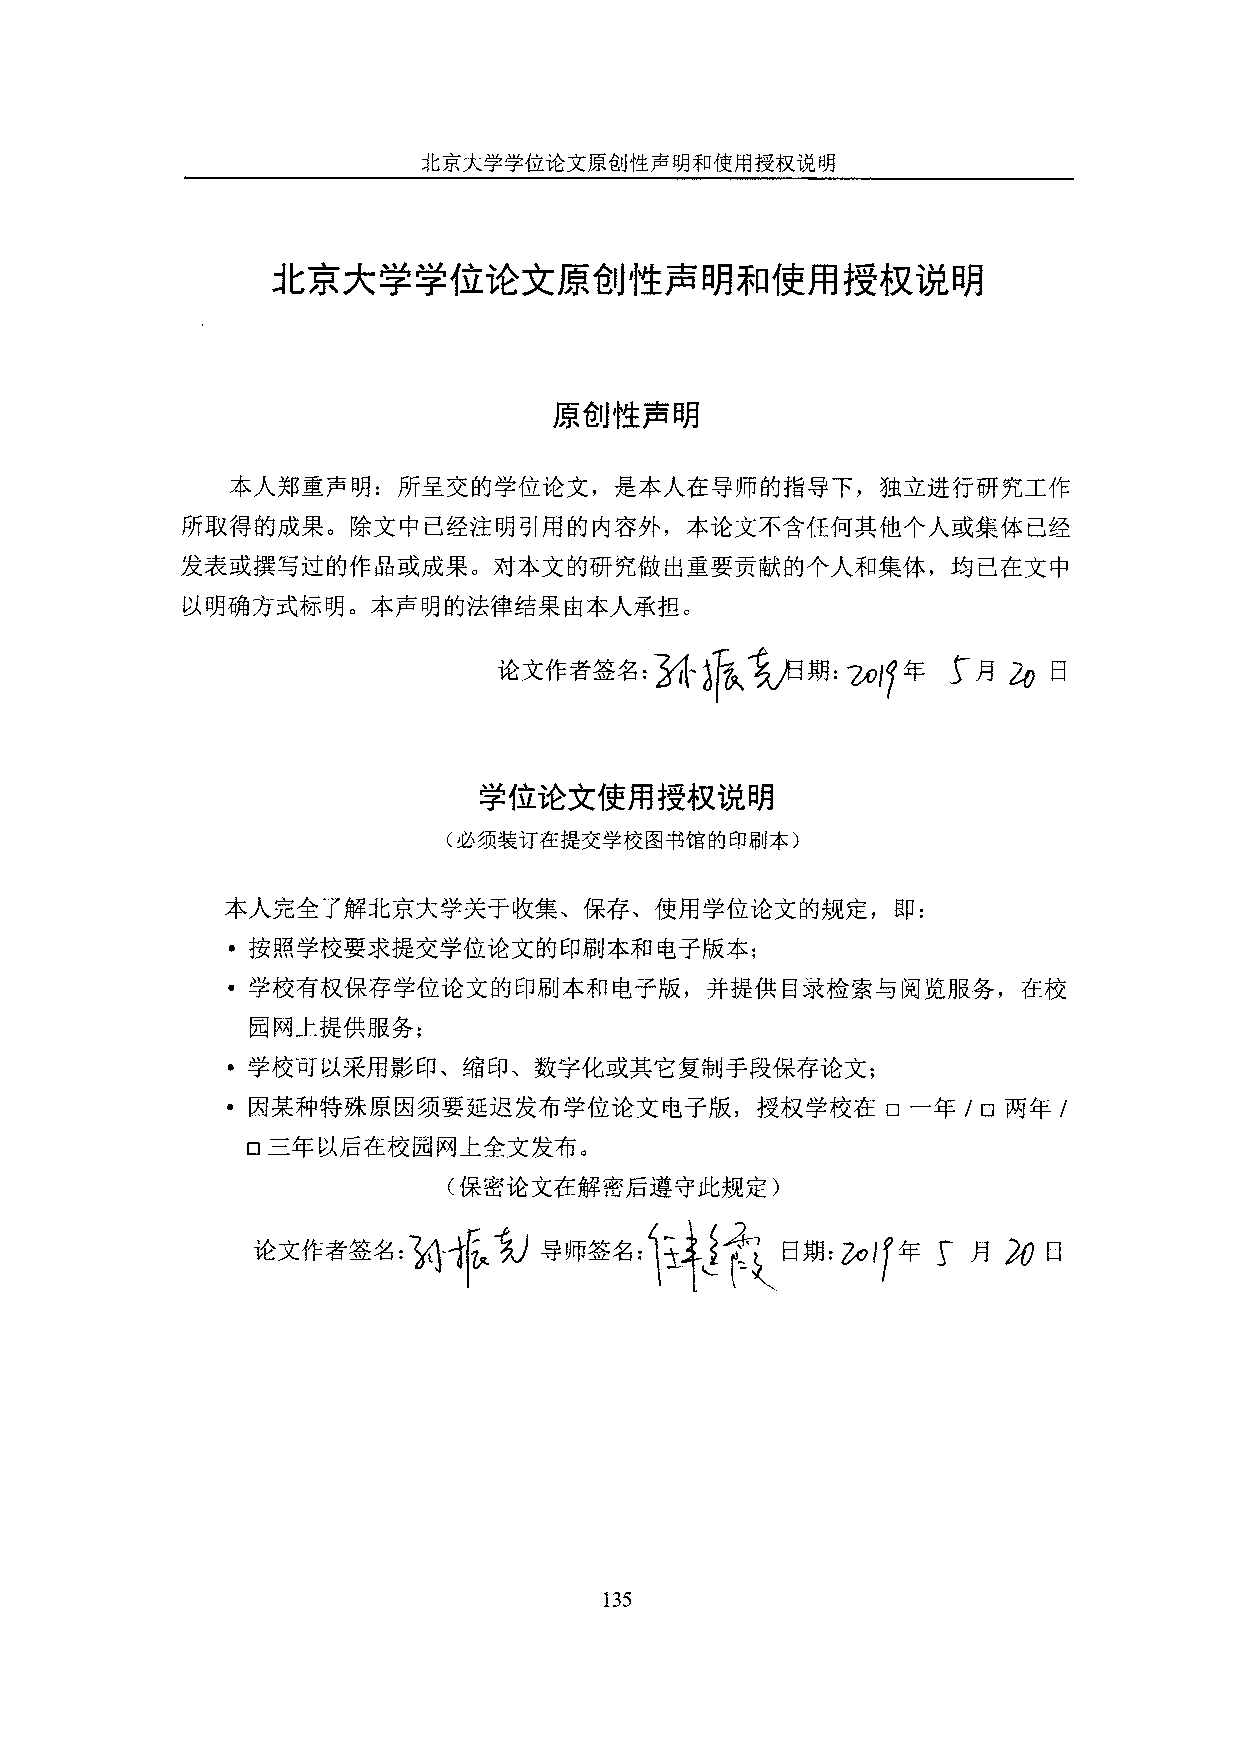
\includepdf[pages={1}]{authorization.pdf}

\begin{comment}	
{
	\ctexset{section = {
		format+ = {\centering}, beforeskip = {40bp}, afterskip = {15bp}
	}}
	\specialchap{北京大学学位论文原创性声明和使用授权说明}
	\mbox{}\vspace*{-3em}
	\section*{原创性声明}

	本人郑重声明:
	所呈交的学位论文,是本人在导师的指导下,独立进行研究工作所取得的成果。
	除文中已经注明引用的内容外,
	本论文不含任何其他个人或集体已经发表或撰写过的作品或成果。
	对本文的研究做出重要贡献的个人和集体,均已在文中以明确方式标明。
	本声明的法律结果由本人承担。
	\vskip 1em
	\rightline{
		论文作者签名:\hspace{5em}%
		日期:\hspace{2em}年\hspace{2em}月\hspace{2em}日%
	}

	\section*{
		学位论文使用授权说明\\[-0.33em]
		\textmd{\zihao{5}(必须装订在提交学校图书馆的印刷本)}%
	}

	本人完全了解北京大学关于收集、保存、使用学位论文的规定,即:
	\begin{itemize}
		\item 按照学校要求提交学位论文的印刷本和电子版本;
		\item 学校有权保存学位论文的印刷本和电子版,
			并提供目录检索与阅览服务,在校园网上提供服务;
		\item 学校可以采用影印、缩印、数字化或其它复制手段保存论文;
		\item 因某种特殊原因须要延迟发布学位论文电子版,
			授权学校在 $\Box$\nobreakspace{}一年 /
			$\Box$\nobreakspace{}两年 /
			$\Box$\nobreakspace{}三年以后在校园网上全文发布。
	\end{itemize}
	\centerline{(保密论文在解密后遵守此规定)}
	\vskip 1em
	\rightline{
		论文作者签名:\hspace{5em}导师签名:\hspace{5em}%
		日期:\hspace{2em}年\hspace{2em}月\hspace{2em}日%
	}
}
\end{comment}
\end{document}

% vim:ts=4:sw=4
